\section{Gaussian simulation study}
\label{sec:simulation_study_gauss}
This section, like \Cref{sec:simulations}, is reproduced from \citet{Arnstad:Relative_variable_importance_in_Bayesian_linear_mixed_models:2024} and is included here for completeness. We present the results of the Gaussian simulation study, where the BVI method is compared to the ELMG, ERW, and Relaimpo methods. The ELMG and ERW methods were implemented by \citet{matre} and the Relaimpo method denotes the LMG method, implemented in the R package \texttt{Relaimpo} \citep{gromping_relaimpo}. Note that the Relaimpo method only considers models without random effects.
% First we compare the fixed effects, and then random effects. Lastly, we consider how our BVI model estimates the conditional and marginal $R^2$ values from a Bayesian perspective, comparing these results to the $R^2$ value obtained from the decompositions by the Relaimpo, ELMG, and ERW methods, where the first method only considers models without random effects. 
\subsection{Relative importance of the fixed effects}
\label{sec:relimp_fixed}
Here, we review the relative importance allocated to each fixed effect from the simulations.
There are four different distributions for each method, which corresponds to the four different correlation levels. 
The horizontal dashed line displays the theoretically correct relative importance from \eqref{eq:RI_theoretical_simulation} when the covariates are pairwise independent. 
\newline
\newline
In general, it can be seen that the distributions in the case of uncorrelated data are unbiased with some variation around the theoretically correct relative importance (\Cref{fig:relimp_all}).
For a correlation of $\rho=0.1$ the distributions of the estimates are shifted marginally compared to the uncorrelated case for all methods.
The importance attributed to $X_1$ and $X_2$, in \Cref{fig:relimp_all}, is larger when compared to the uncorrelated case, whereas the importance attributed to $X_3$ is smaller.
All methods seem to shift the relative importance estimate for the covariate with the same amount in the same direction.
This shift is both expected and desirable, when considering the values found in \Cref{table:2} for the theoretically correct variance explained. 
Therefore, we should expect our method to assign different shares when we have various levels of covariate correlation, which it does.
This trend continues for the correlation level $\rho=0.5$, where the distributions are shifted further in the same directions as for $\rho=0.1$.
Lastly, for $\rho=0.9$ we see the largest reallocation of the distributions, which follows the same trend as for the other correlation levels.
\newline
\newline
The rise in importance for $X_1$ and $X_2$ for increasing correlation can be understood by the relation $\mathbf{Z}\boldsymbol{\Lambda}=\mathbf{X}$ in the relative weights method. 
When the matrix $\mathbf{X}$ is not correlated, $\boldsymbol{\Lambda}$ is close to the identity matrix, but with an increase in correlation the diagonal elements grows smaller and off diagonal elements grow larger.
An increase in off diagonal values would for $X_1$ and $X_2$ imply that a larger value is multiplied with $\beta_3^2$, which is larger than $\beta_1^2$ and $\beta_2^2$. 
Therefore, it is expected to see a rise in importance as correlation increases for $X_1$ and $X_2$, and the opposite for $X_3$.
In all figures, the BVI method is in agreement with the other methods when allocating importance for different correlation levels.
The width of the distributions seem to become lower as the correlation increases, most notably for $\rho=0.9$, where the distributions exhibit significantly smaller dispersion than for $\rho=0$.
Generally all methods seem to follow the same trends and produce similar results for all three fixed effects. 
As correlation increases the trend is that the relative importance assigned to $X_1$ and $X_2$ increases, in contrast to the decrease in relative importance assigned to $X_3$.
\newline
\newline
In general, the BVI method is in agreement with the theoretical results for uncorrelated data derived in \Cref{ch:method} and is consistent with the other three methods for correlated fixed effects. 
\begin{figure}[H]
  \centering
  %\label{fig:relimp_all}
  \begin{subfigure}[b]{0.7\linewidth}
    \centering
    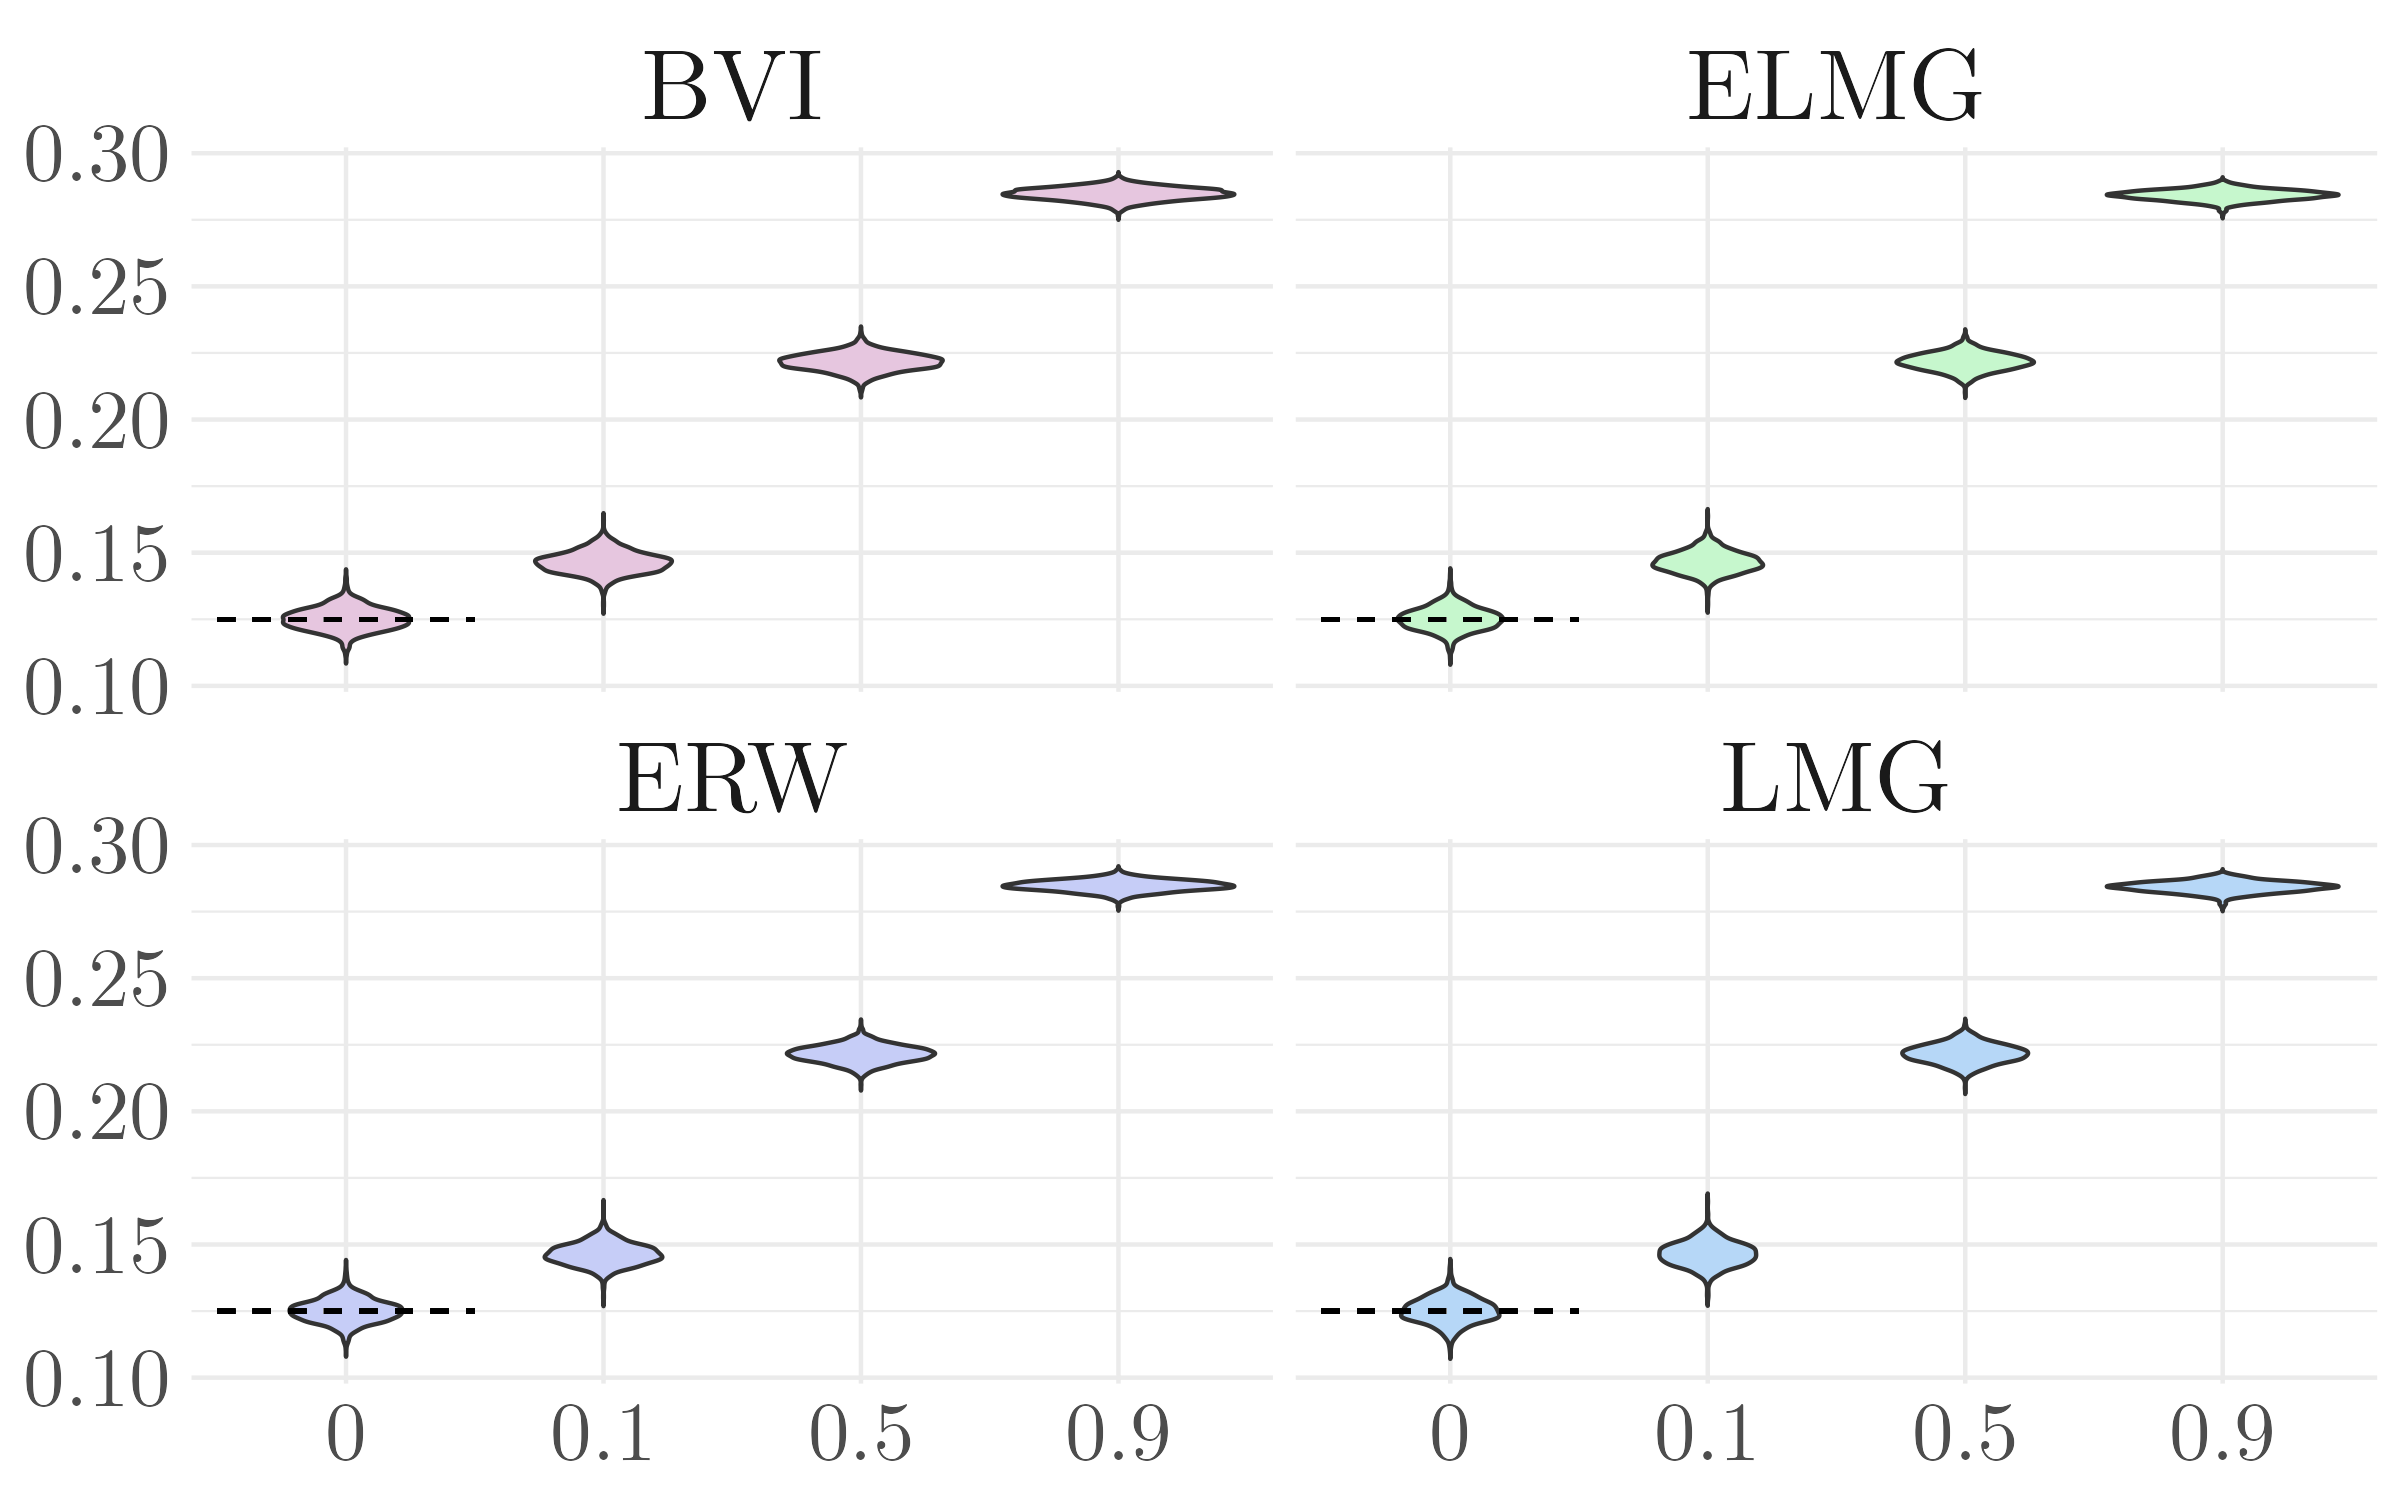
\includegraphics[width=\linewidth]{Figures/ViolinPlots/Variance_V1.png}
    %\caption{Relative importance of $X_1$ as calculated from the four methods.}
    \label{fig:relimp_X1_fig}
  \end{subfigure}
  
  \begin{subfigure}[b]{0.7\linewidth}
    \centering
    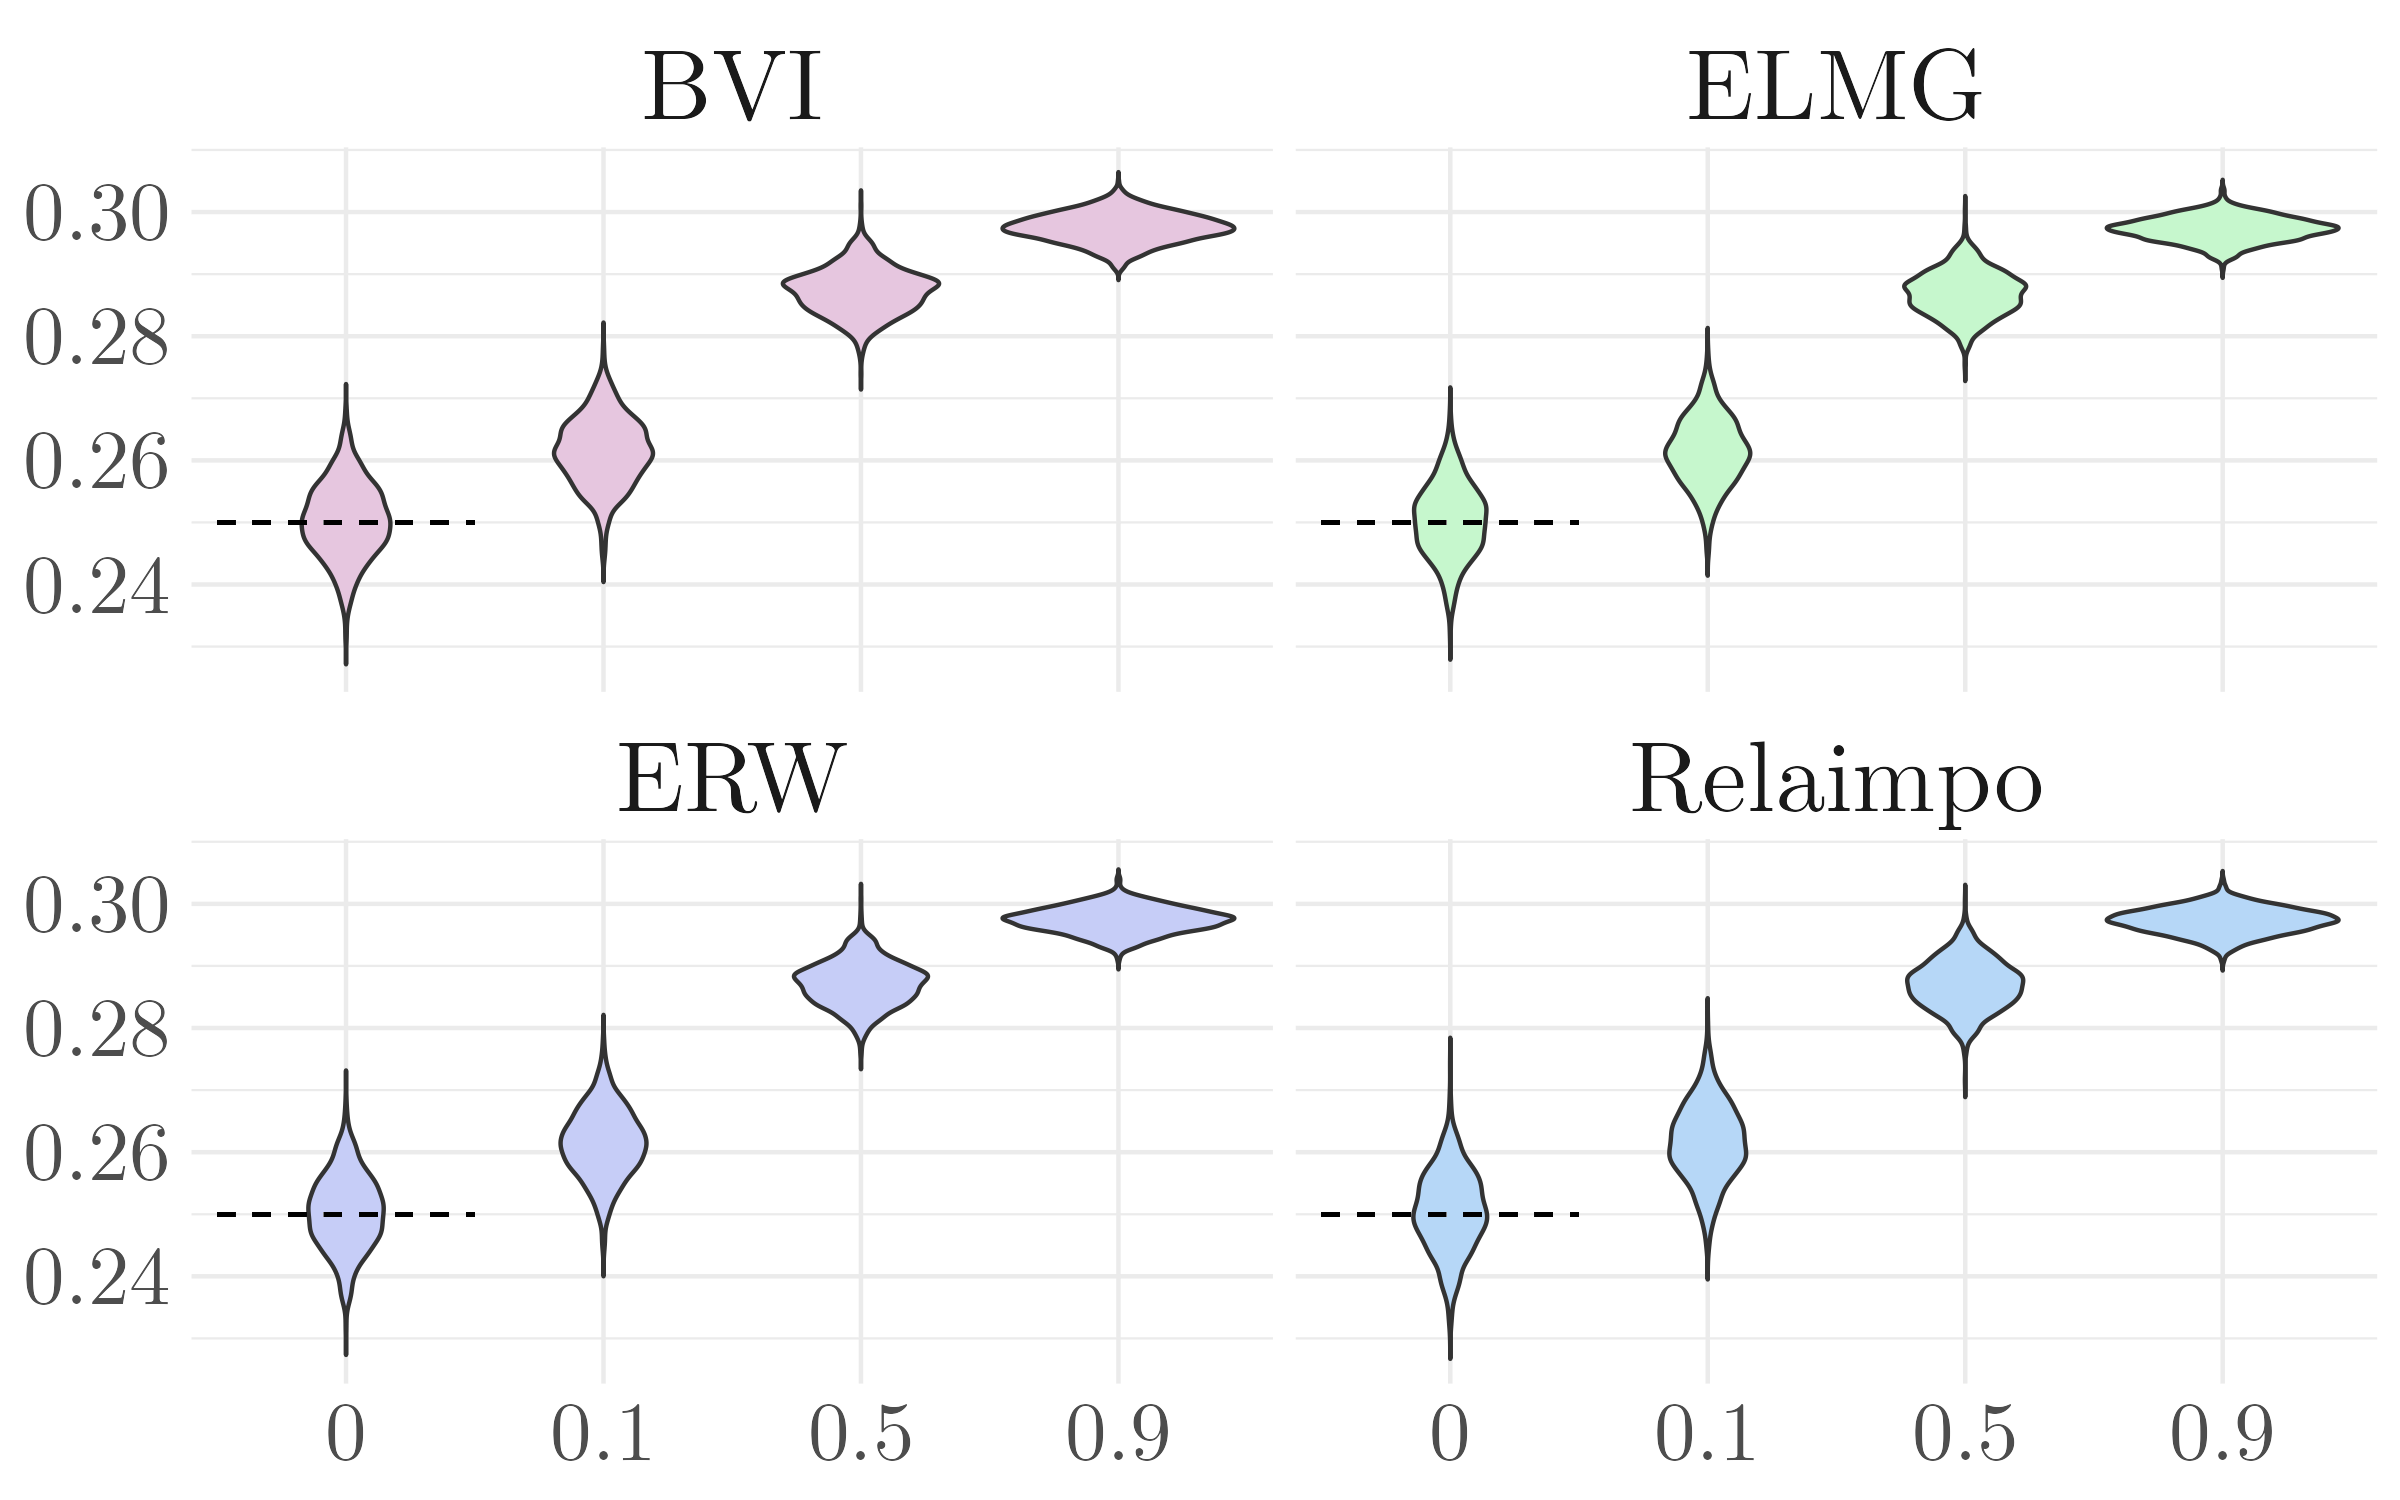
\includegraphics[width=\linewidth]{Figures/ViolinPlots/Variance_V2.png}
   %\caption{Relative importance of $X_2$ as calculated from the four methods.}
    \label{fig:relimp_X2_fig}
  \end{subfigure}
  
  \begin{subfigure}[b]{0.7\linewidth}
    \centering
    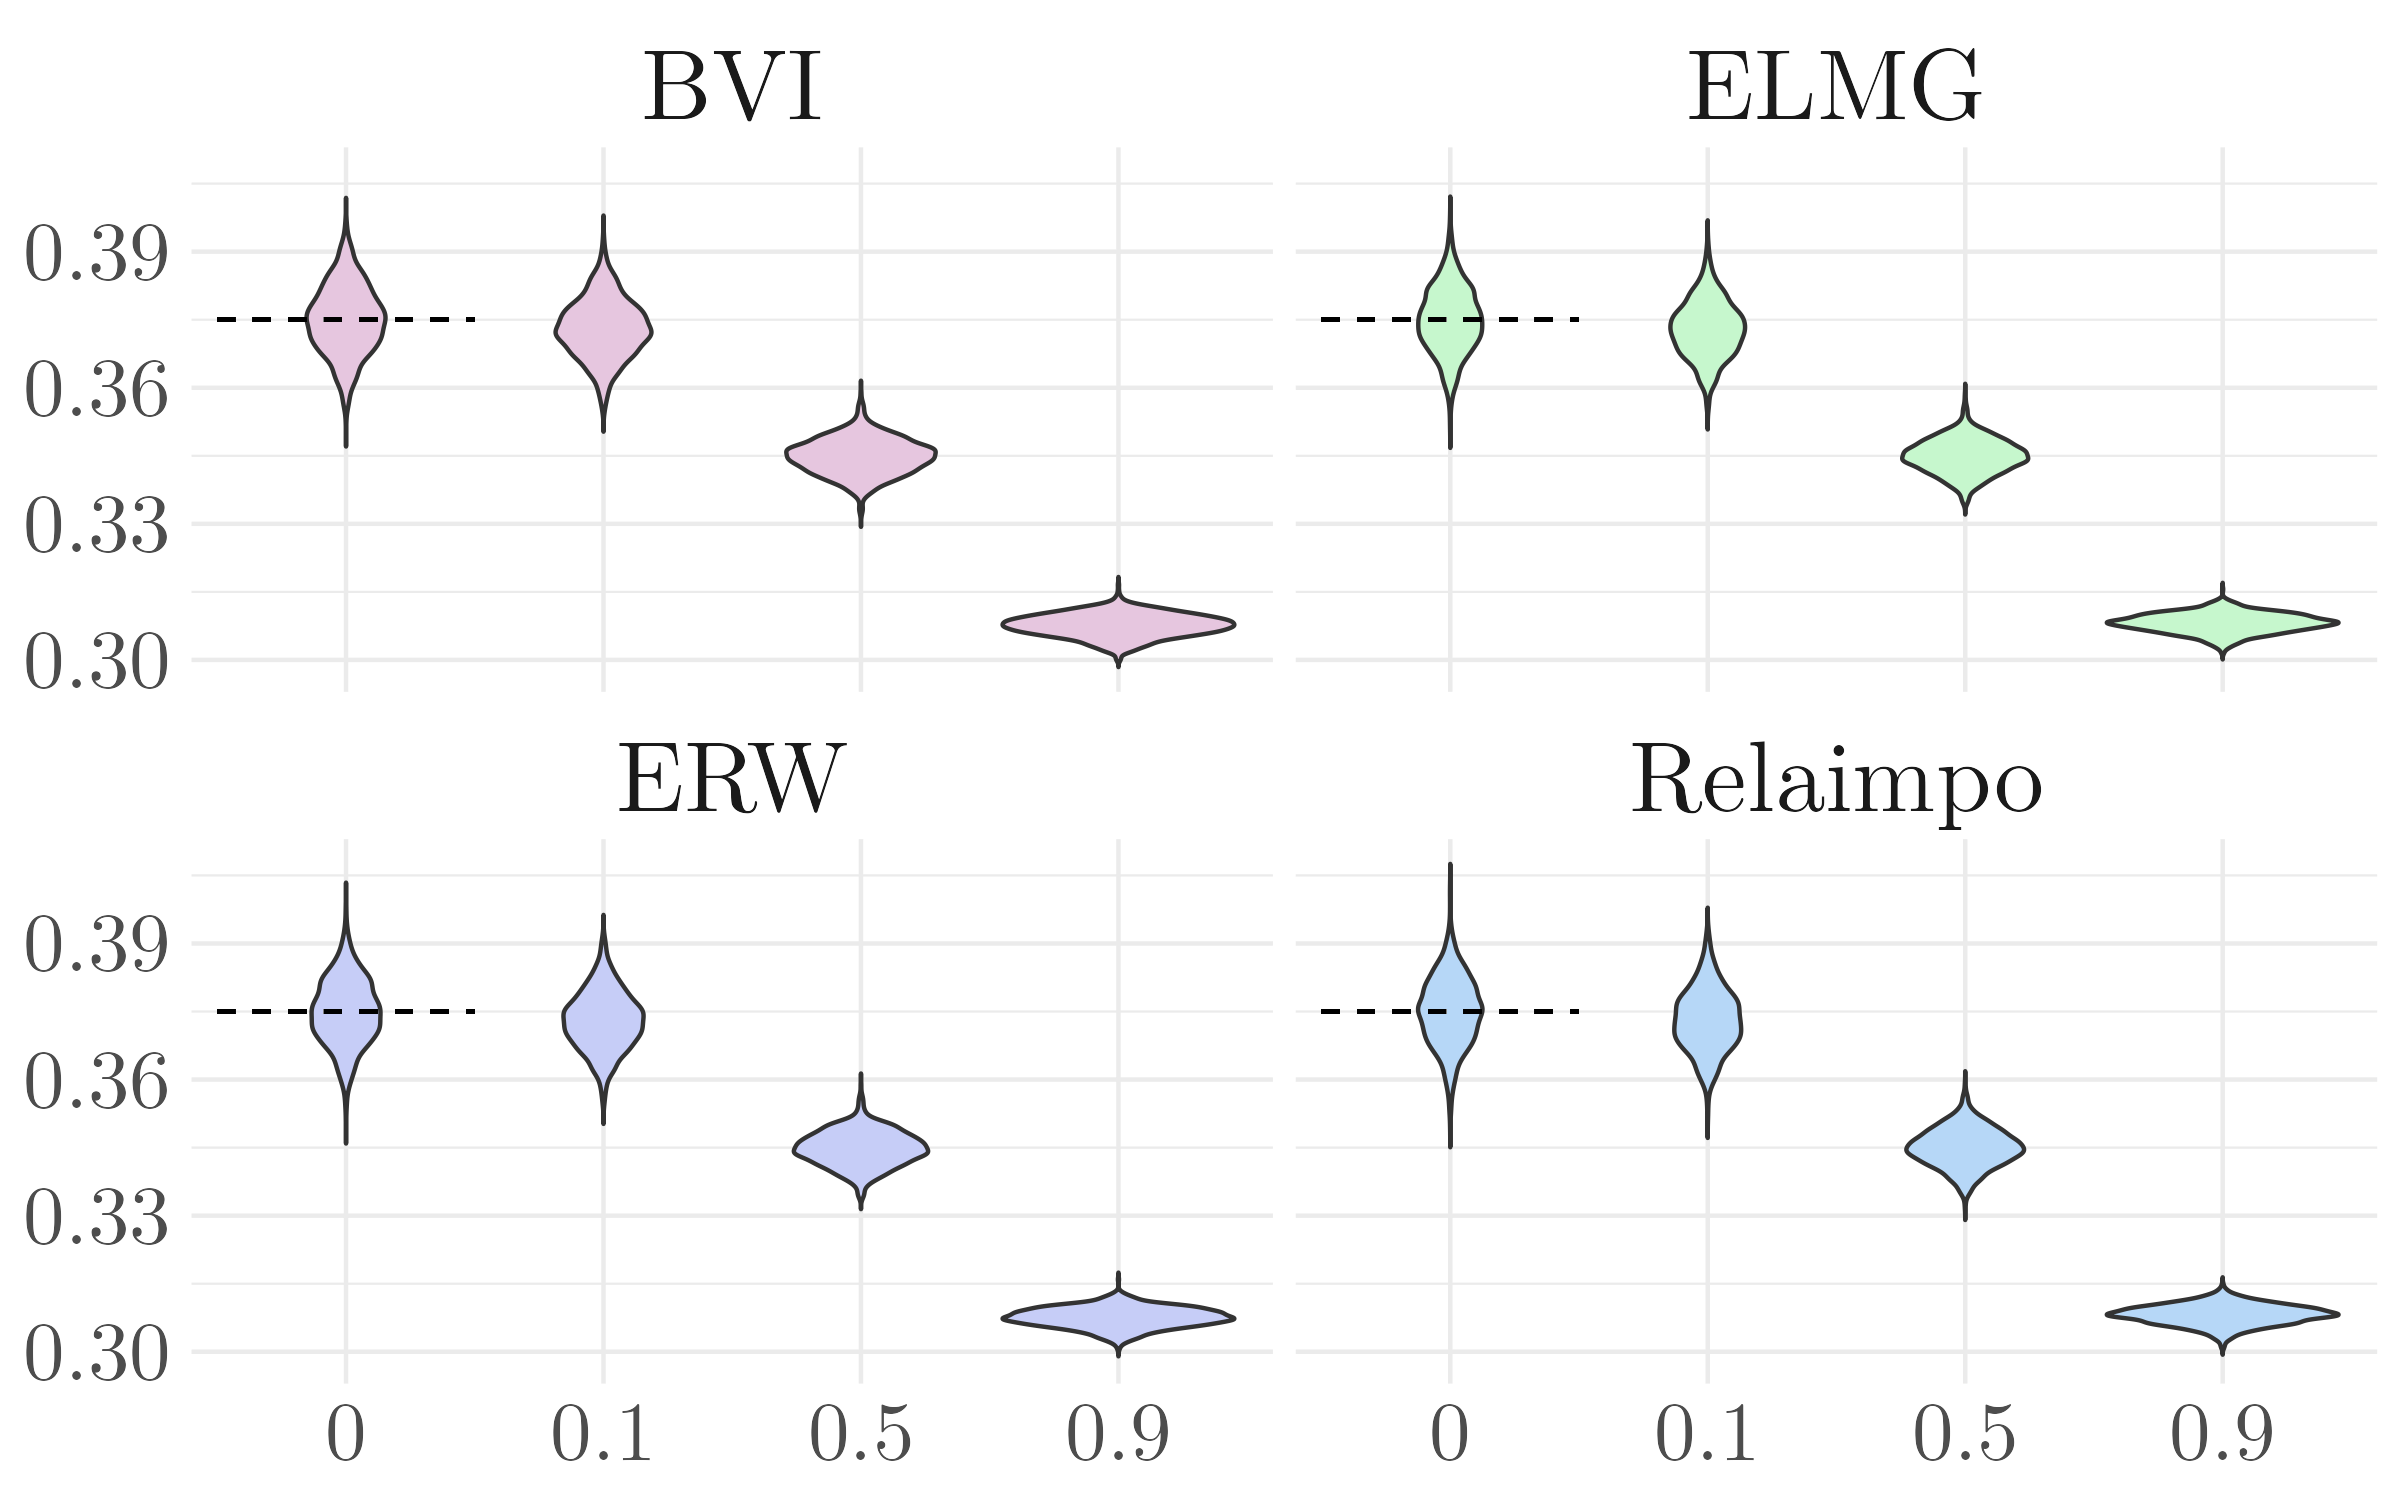
\includegraphics[width=\linewidth]{Figures/ViolinPlots/Variance_V3.png}
    %\caption{Relative importance of $X_3$ as calculated from the four methods.}
    \label{fig:relimp_X3_fig}
  \end{subfigure}
  
  \caption[Relative importance of the fixed effects in Gaussian LMM]{Violin plots for the relative importance of the fixed effects $X_1$ (top), $X_2$ (middle) and $X_3$ (bottom) for different correlation levels displayed along the x-axis, calculated from the ensemble of simulated datasets by the BVI, ELMG, ERW, and the Relaimpo methods. The horizontal line displays the theoretically correct importance of each fixed effect in the case of uncorrelated data. For the BVI method, the distributions of posterior means are shown to compare to the distribution of point estimates from the other three methods. }
  \label{fig:relimp_all}
\end{figure}

% \begin{figure}[H]
%   \centering
%     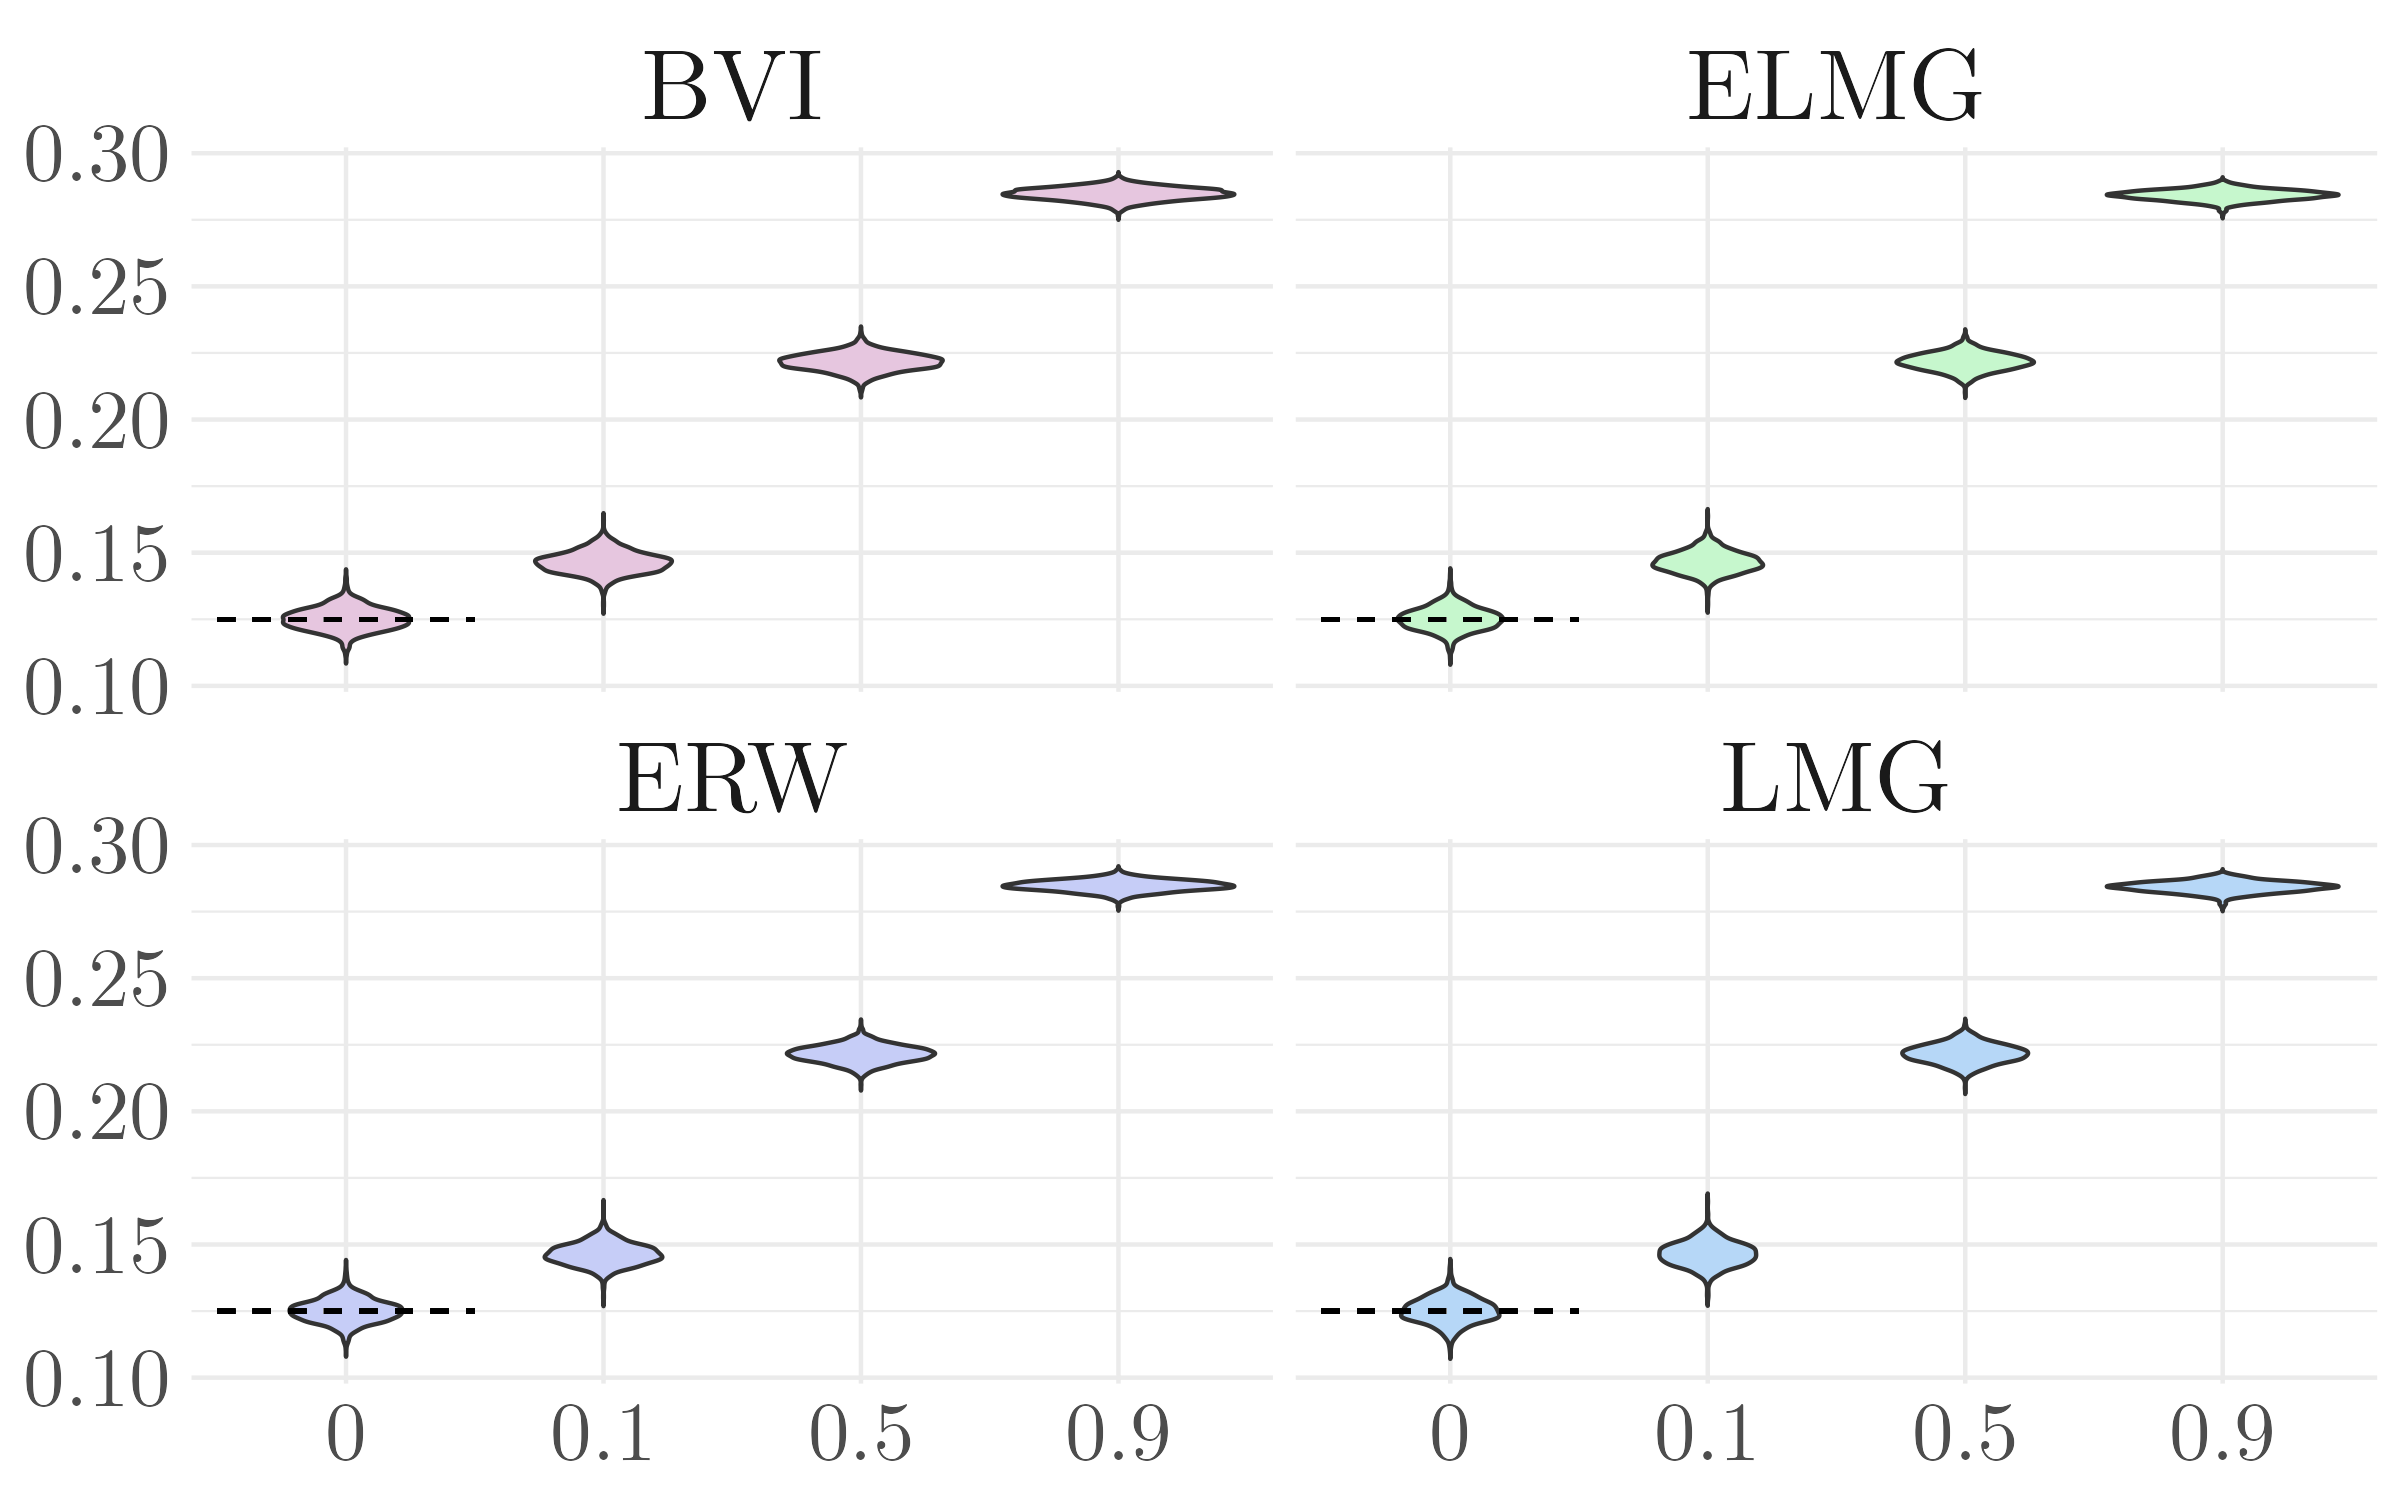
\includegraphics[width=0.7\linewidth]{Figures/ViolinPlots/Variance_V1.png}
%     \caption{Violin plots for the relative importance of the fixed effects $X_1, X_2$ and $X_3$ for different correlation levels calculated from the ensemble of simulated datasets by the BVI, ELMG, ERW and the Relaimpo methods. The standardized regressor coefficients are $\boldsymbol{\beta}=\left(\sqrt{1/8}, \sqrt{2/8}, \sqrt{3/8}\right)$, and the true total model variance is $\sigma^2_{\mathbf{y}}=1$. For the BVI method the distributions of posterior means are shown to compare to the distribution of point estimates from the other three methods. The horizontal line displays the theoretically correct importance of each fixed effect in the case of uncorrelated data. (a) Relative importance of $X_1$ as calculated from the four methods.}
%     \label{fig:relimp_X1}
% \end{figure}
% \begin{figure}[H]\ContinuedFloat
%   \centering
%     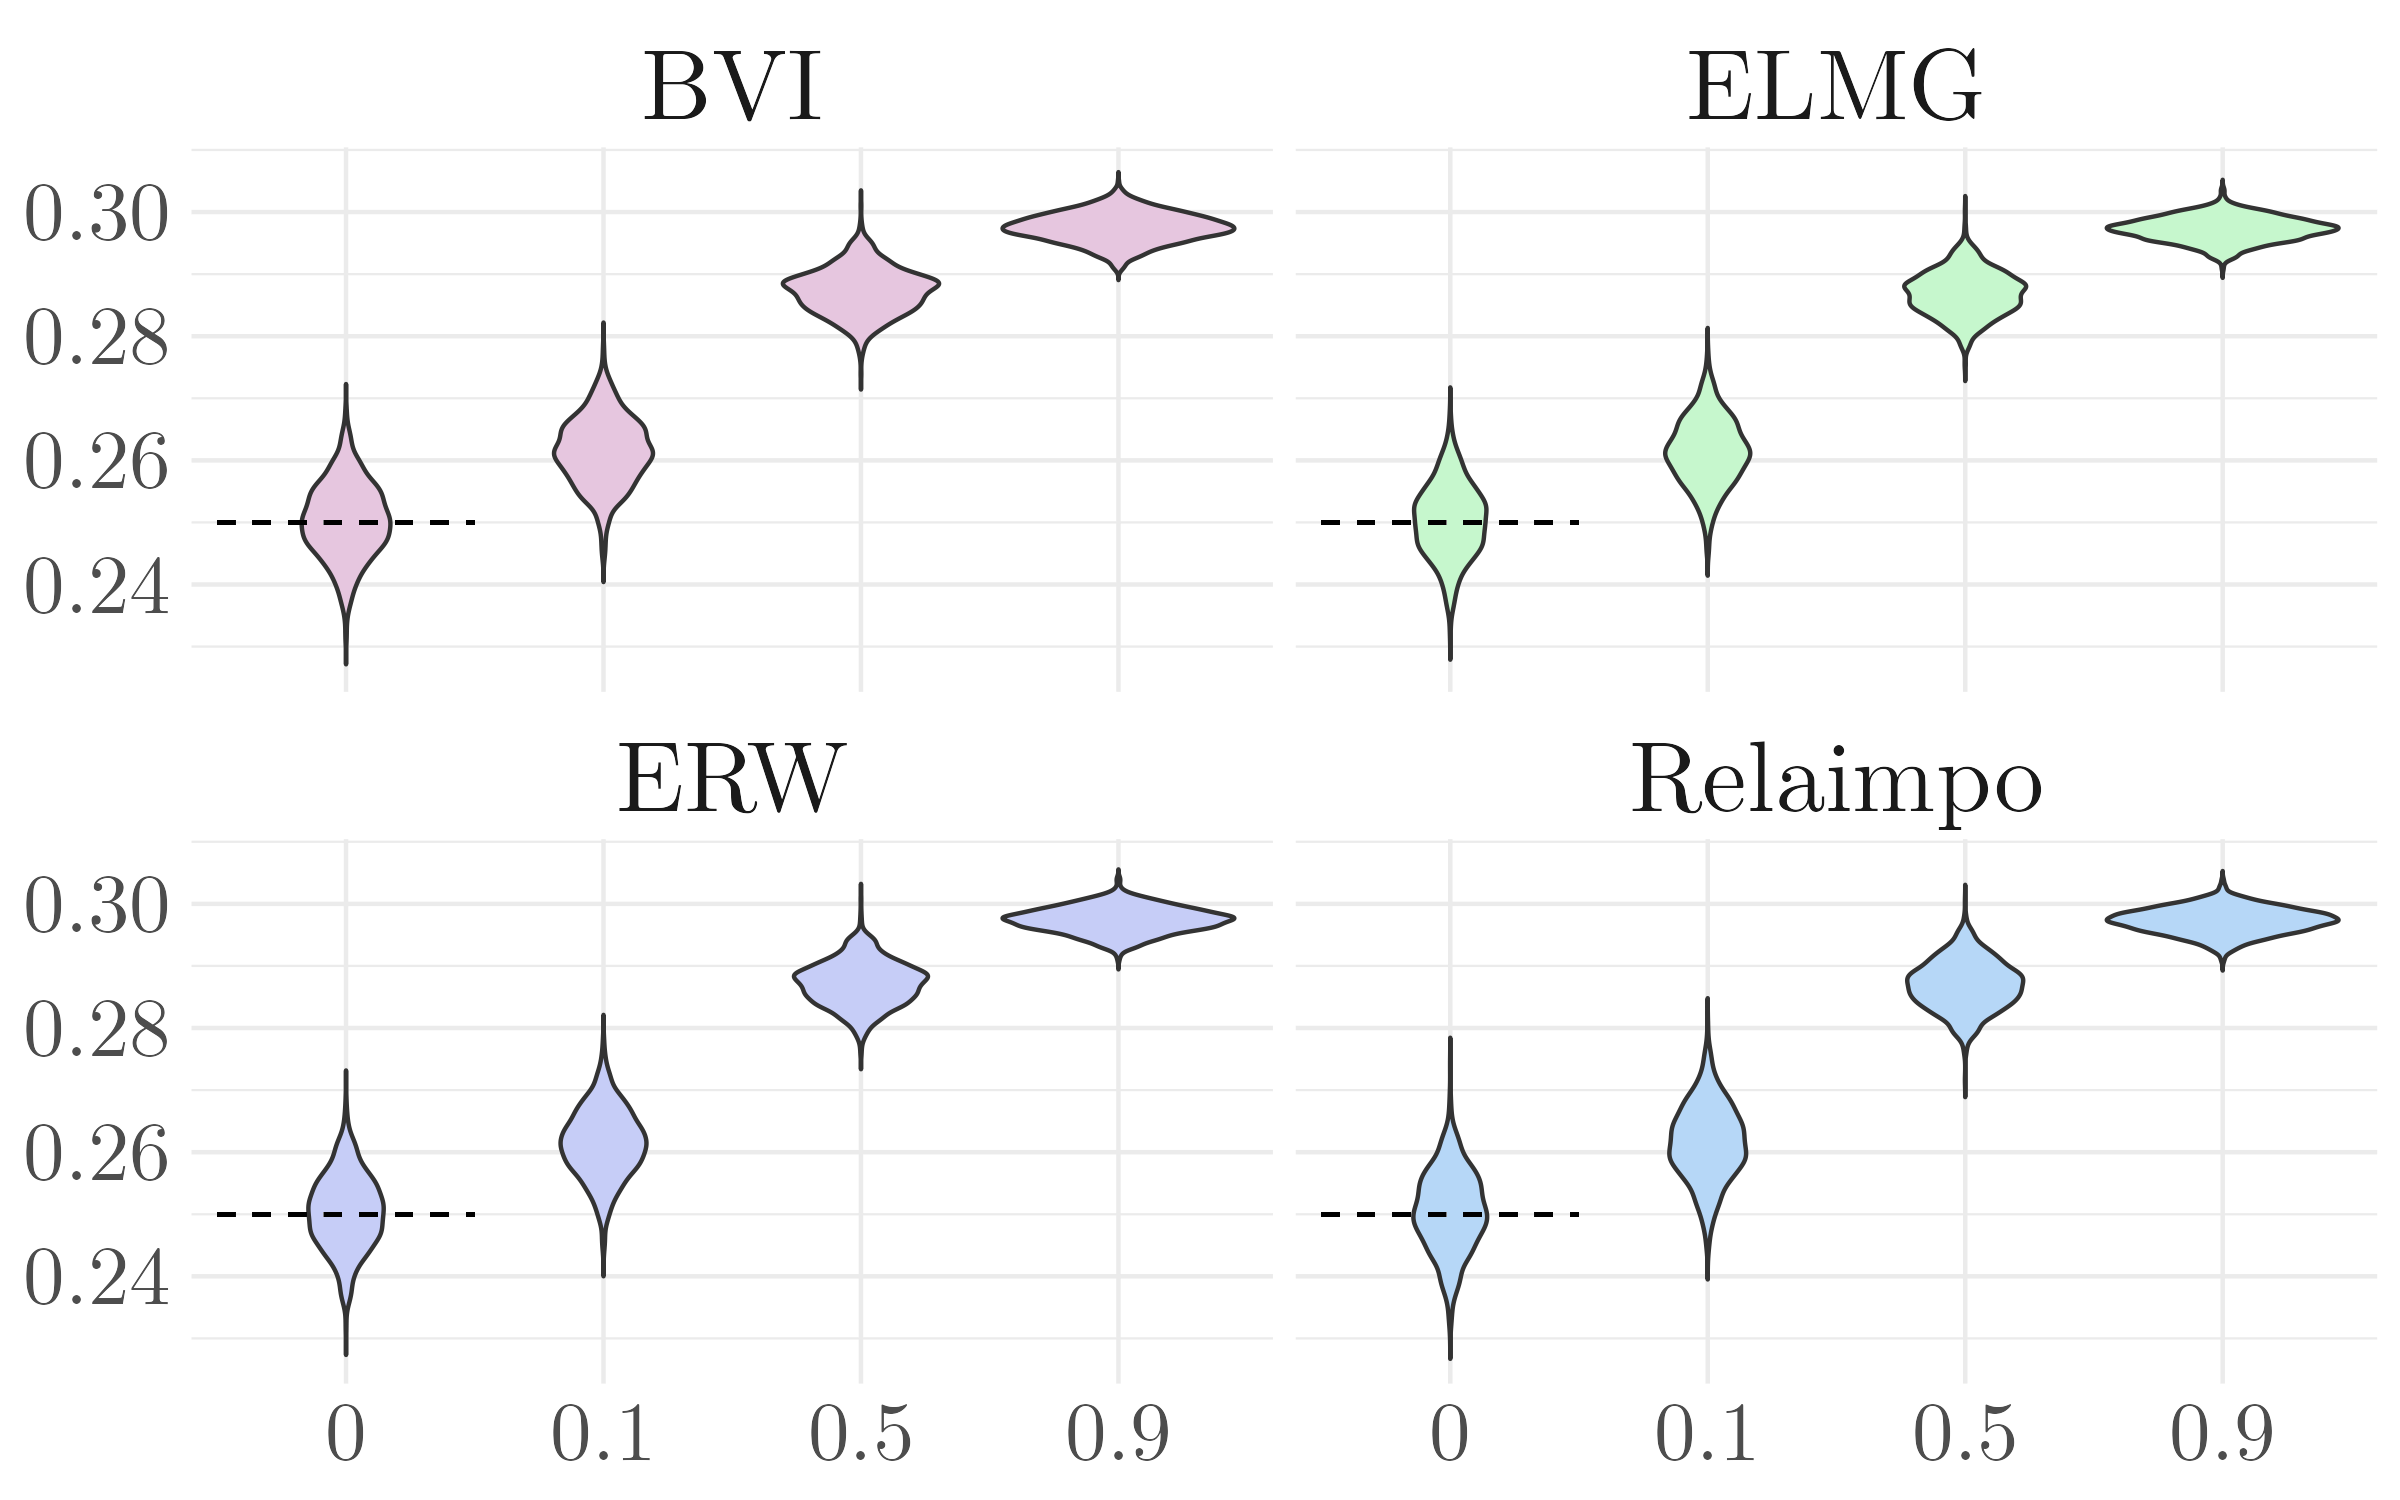
\includegraphics[width=0.7\linewidth]{Figures/ViolinPlots/Variance_V2.png}
%     \caption{(b) Relative importance of $X_2$ as calculated from the four methods.}
%     \label{fig:relimp_X2}
% \end{figure}
% \begin{figure}[H]\ContinuedFloat
%   \centering
%     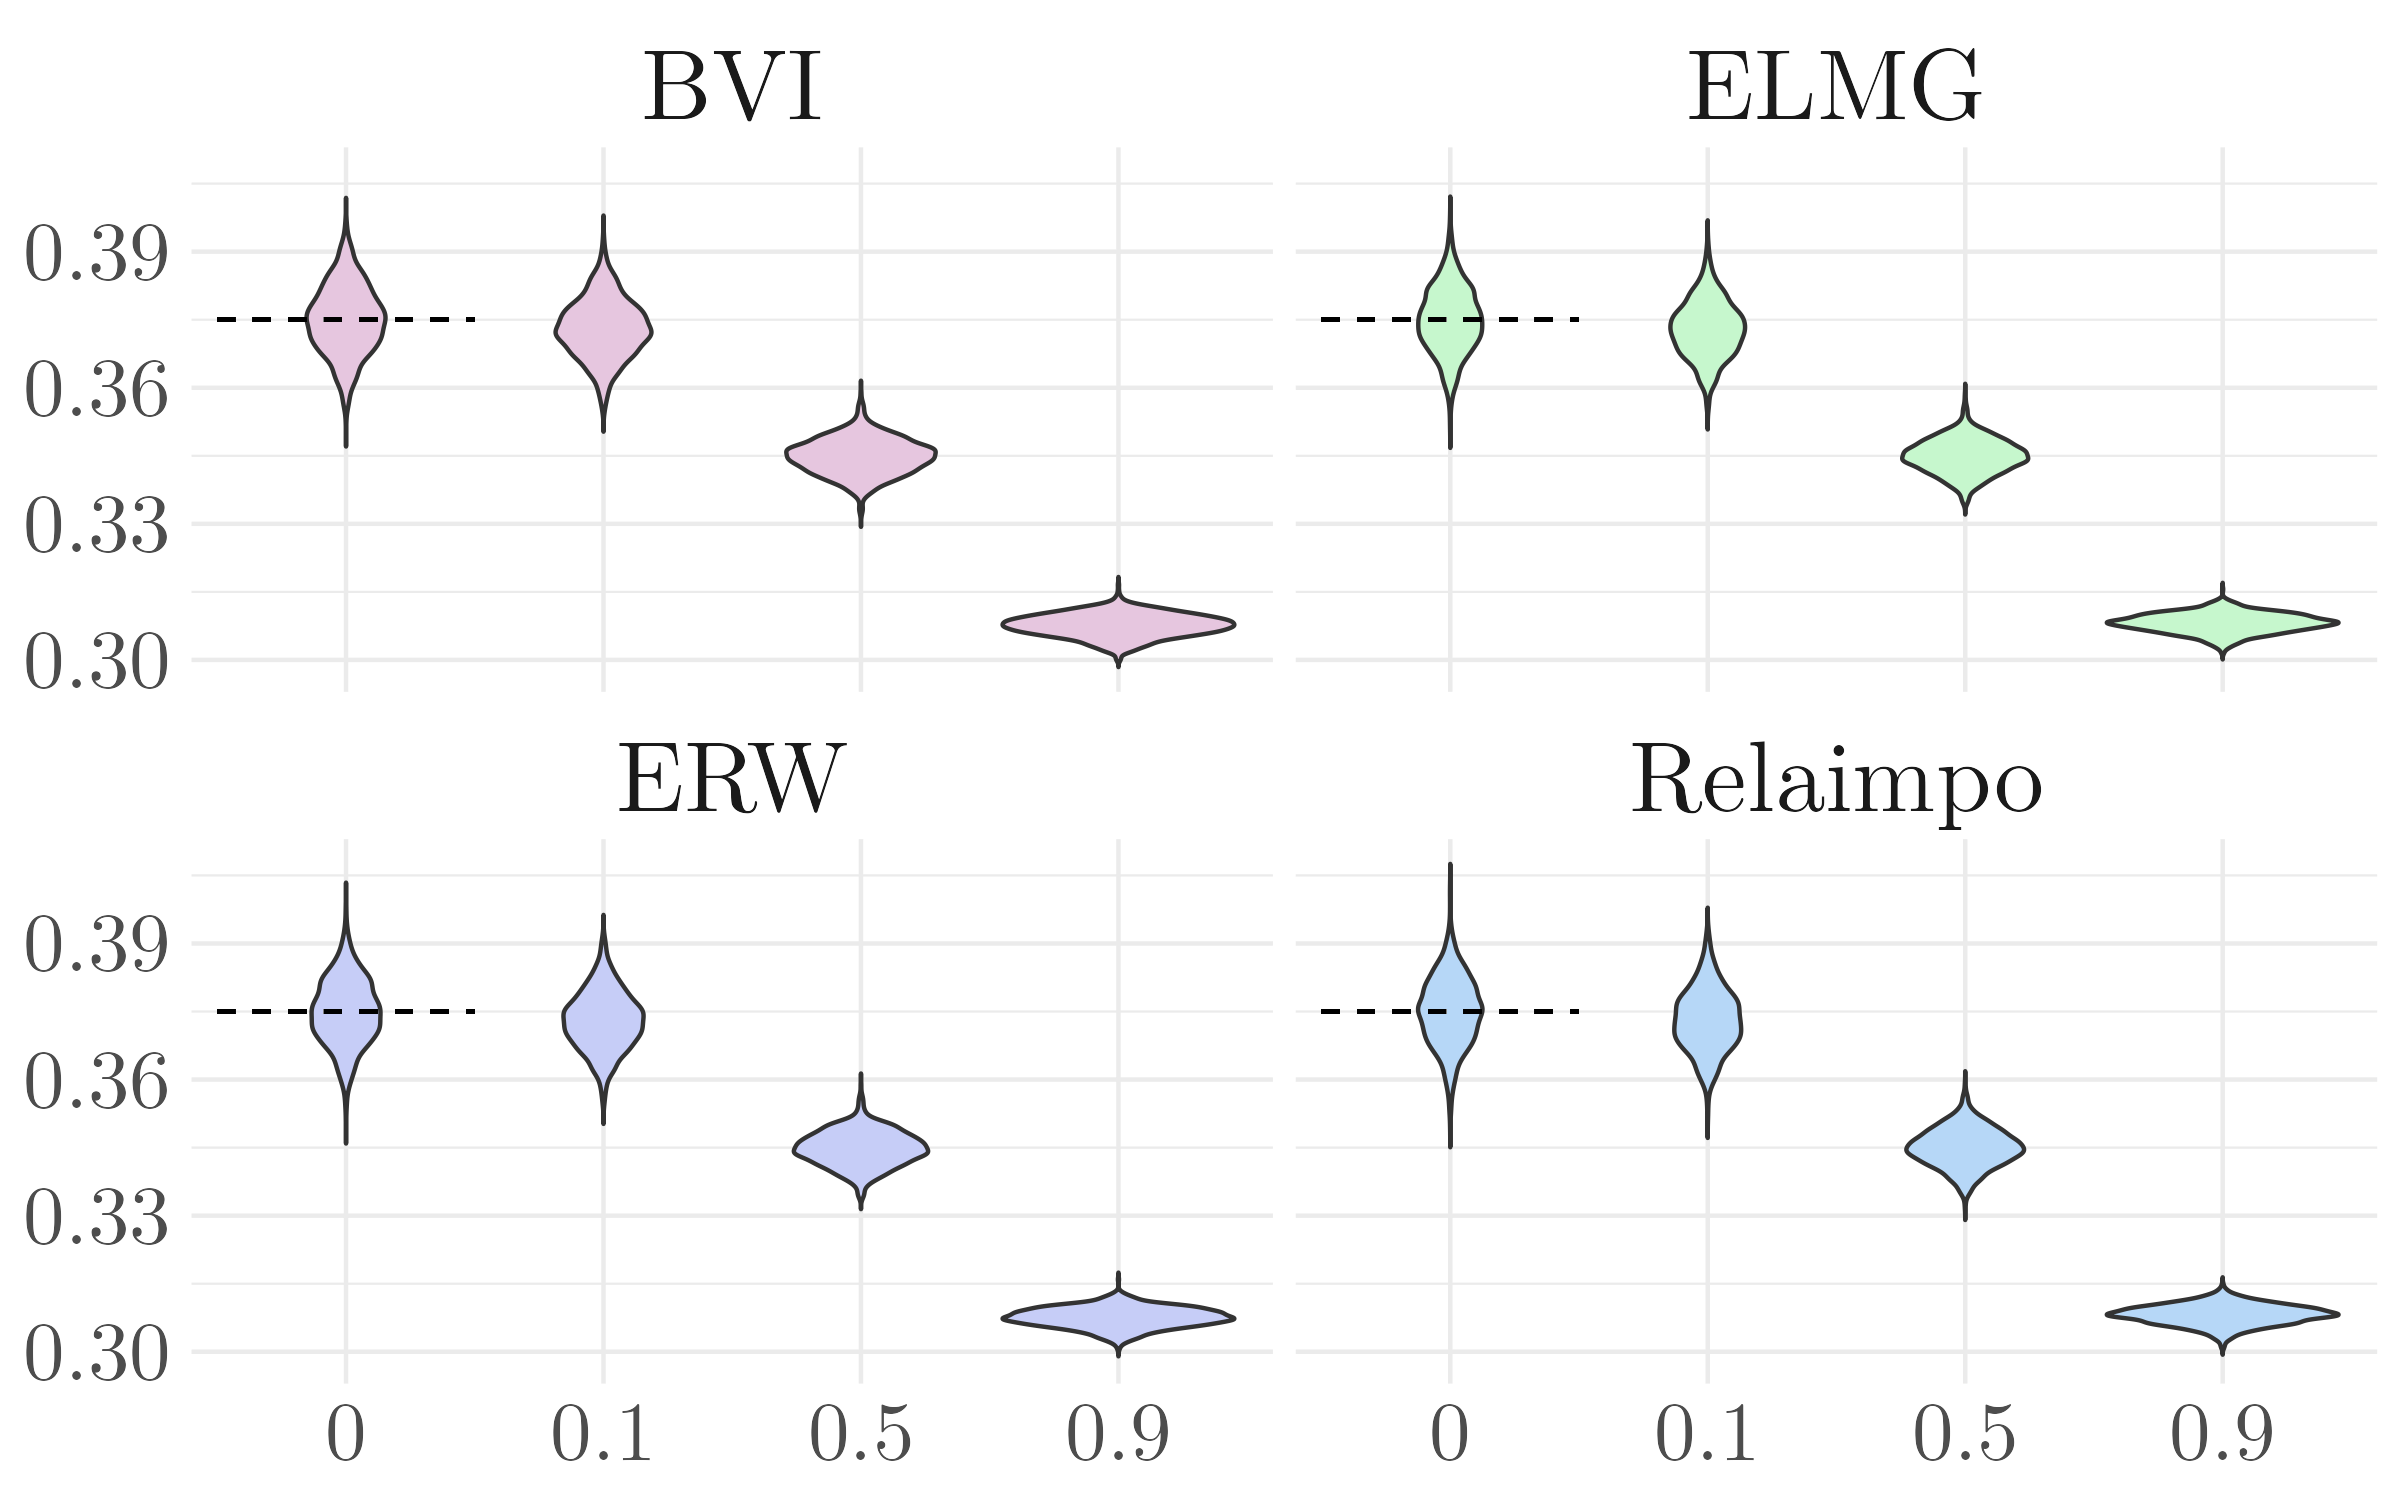
\includegraphics[width=0.7\linewidth]{Figures/ViolinPlots/Variance_V3.png}
%     \caption{(c) Relative importance of $X_3$ as calculated from the four methods.}
%     \label{fig:relimp_X3}
% \end{figure}

\subsection{Relative importance of the random effects}
\label{sec:relimp_random}
Considering a model with one random intercept, we can no longer compare our model with the Relaimpo method, which is only implemented for the linear regression in the Relaimpo R package \citep{gromping_relaimpo}. Therefore, we now compare the BVI method only with the ELMG and ERW methods, which have been extended from the Relaimpo method \citep{matre}.
We display (\Cref{fig:relimp_alpha}) the distribution of the relative importance, or variance, assigned to the random intercept $\boldsymbol{\alpha}$ for different correlation levels. 
The random intercept $\boldsymbol{\alpha}$ follows a univariate normal distribution with mean zero and variance equal to $1$.
As before the horizontal line shows the theoretical relative importance from \eqref{eq:RI_theoretical_simulation} that $\boldsymbol{\alpha}$ has in the model when the fixed effects are uncorrelated.
\newline
\newline
It is apparent (\Cref{fig:relimp_alpha}) that both the location and width of the relative importance distribution of all methods are largely indistinguishable. 
The distributions take on a moderately smaller value when $\rho=0.1$ and the location of the estimates is further decreased for $\rho=0.5$ and $\rho=0.9$. 
For the latter correlation level, the distributions are located around a value that is less than half of the value of the centering when the fixed effects are uncorrelated. 
To re-emphasize, this is both expected and desirable since the increase in response variance comes solely from the correlation of fixed effects, so the random effects now contribute to explain a smaller proportion of the variance, \textit{i.e.} the importance is lower.
\begin{figure}[ht]
  \centering
  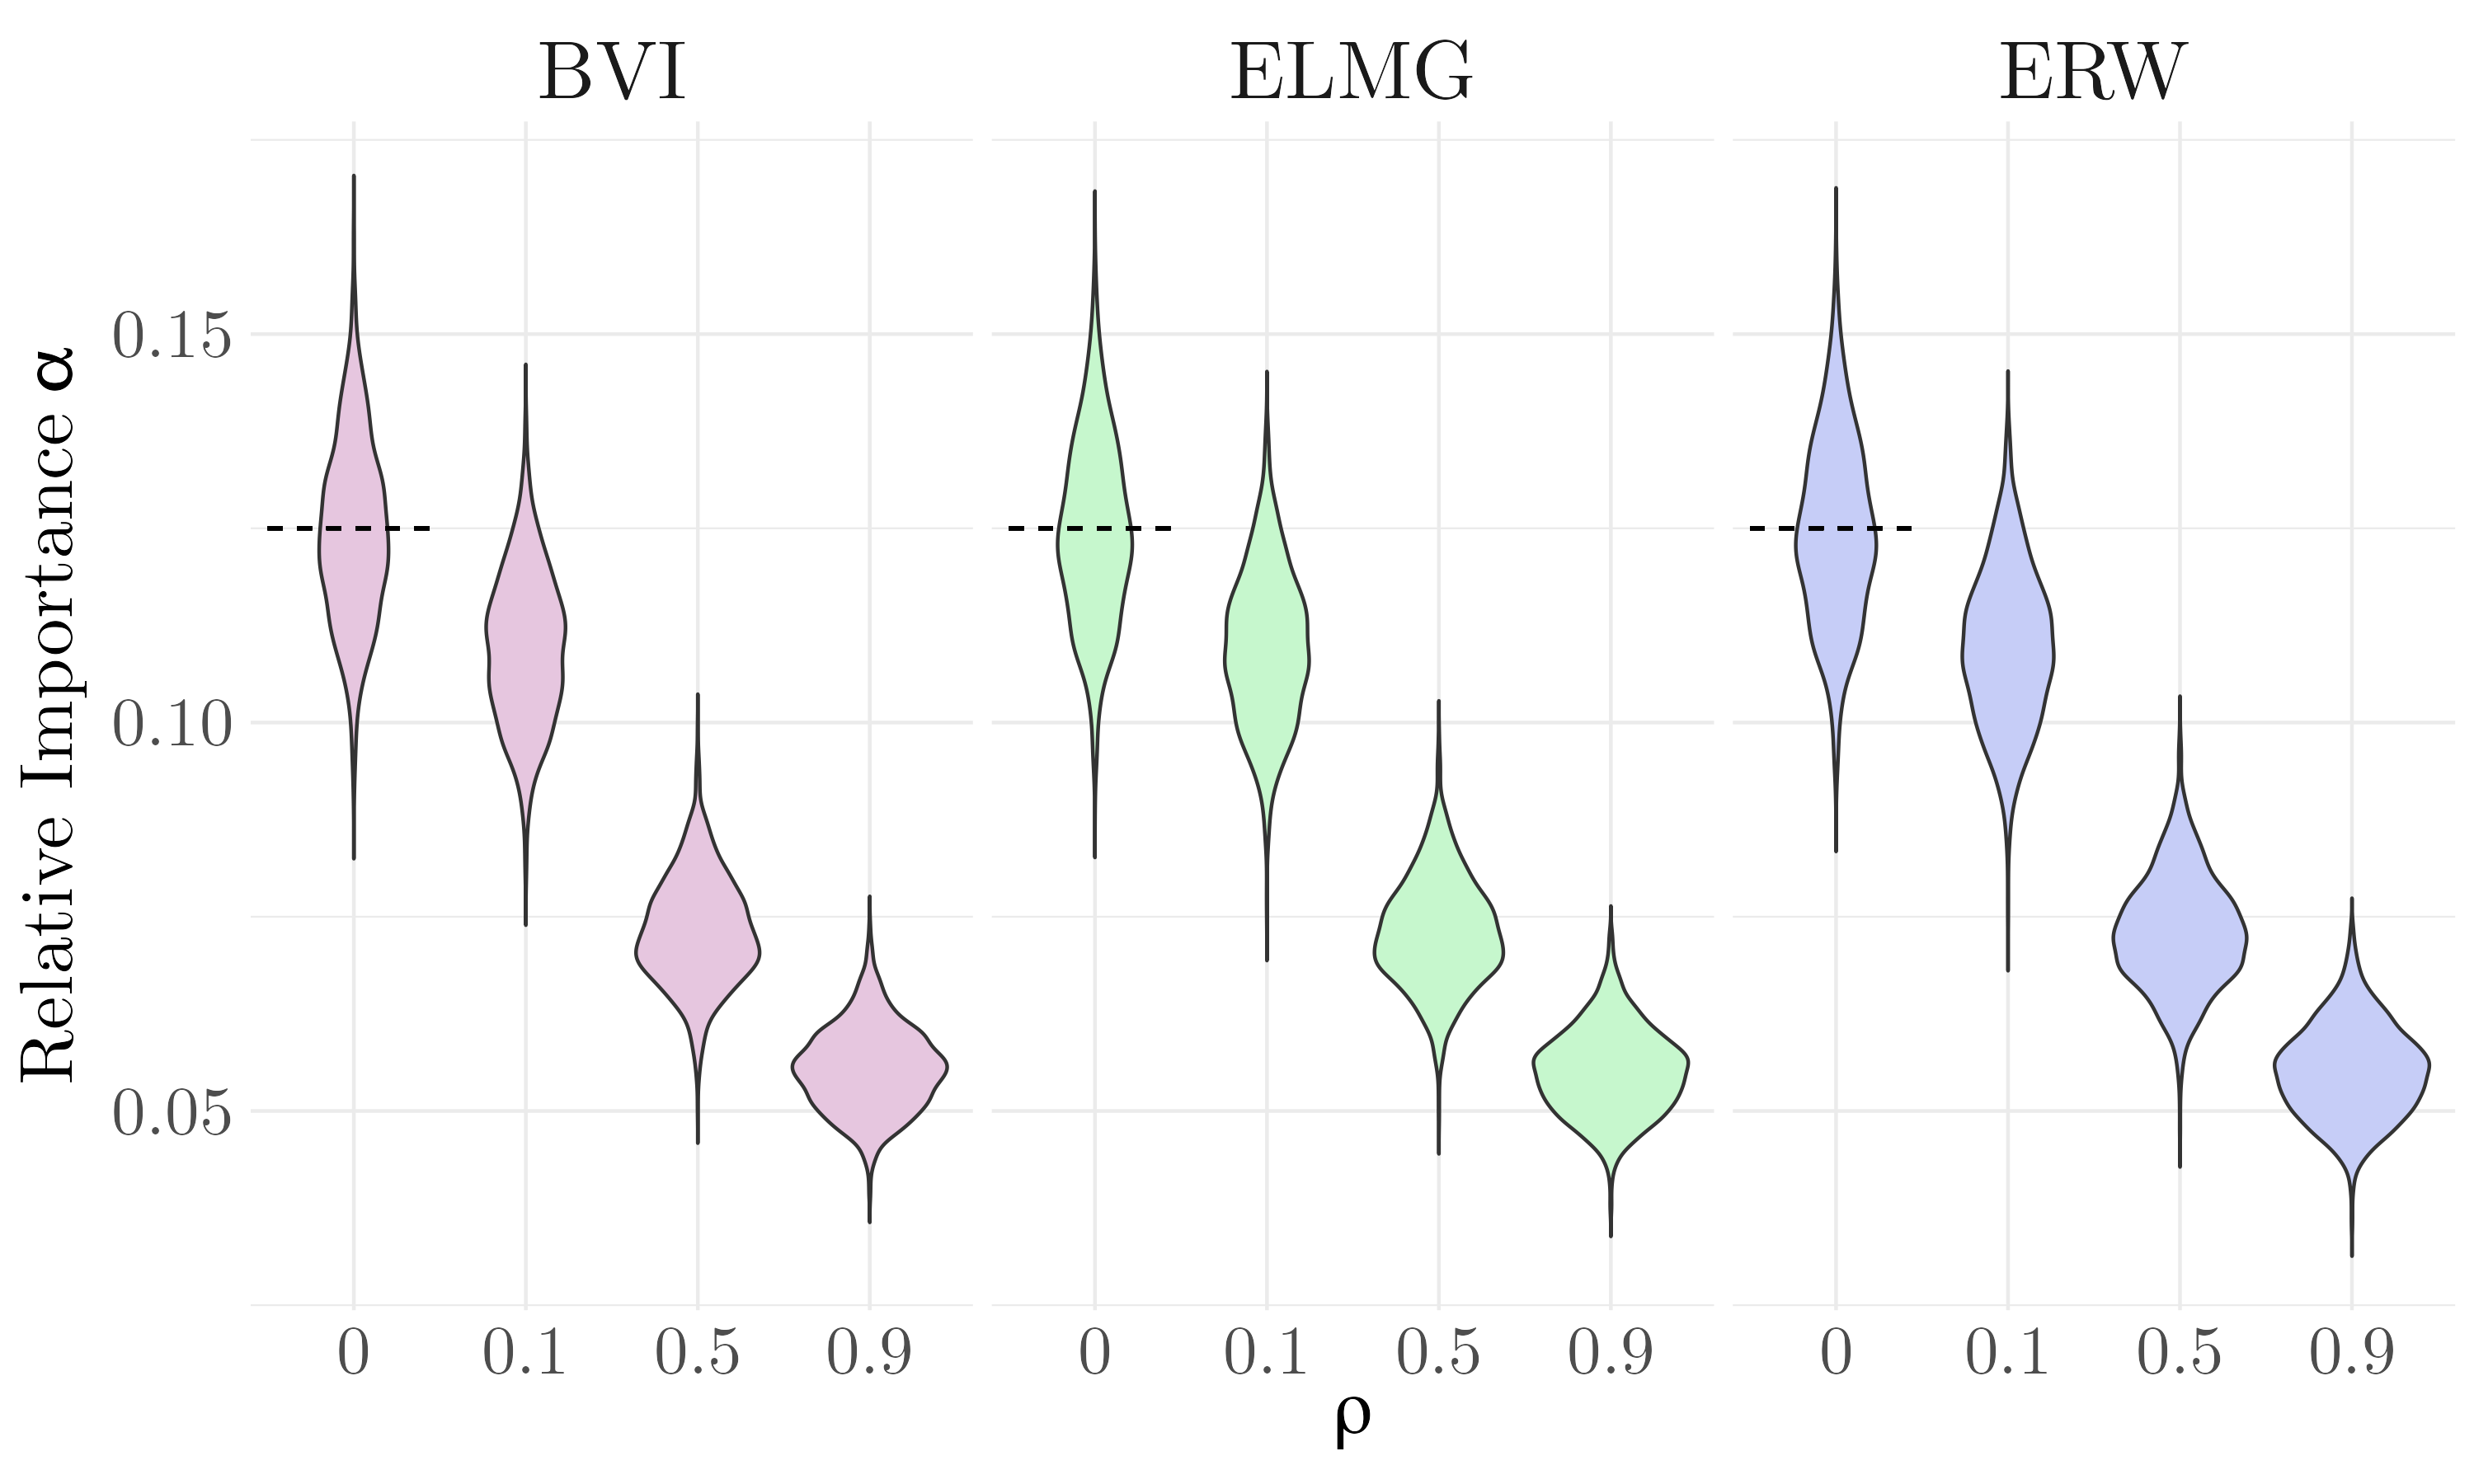
\includegraphics[width=0.7\linewidth]{Figures/ViolinPlots/Variance_gamma.png}
  \caption[Relative importance of the random effect $\boldsymbol{\alpha}$ in Gaussian LMM]{Violin plots for the relative importance of the random effect $\boldsymbol{\alpha}$, that is, $\hat{\sigma}^2_{\alpha}$ for different correlation levels displayed along the x-axis, calculated from the ensemble of simulated datasets by the BVI, ELMG and the ERW method. For the BVI method the distributions of posterior means of the marginal distribution of $\hat{\sigma}^2_{\alpha}$ are shown to compare to the point estimates of the other two methods. The horizontal line displays the theoretically correct importance $\sigma^2_{\alpha}$ of the random effect in the case of uncorrelated data.}
  \label{fig:relimp_alpha}
\end{figure}

\subsection{Total variance explained - \texorpdfstring{$R^2$}{Lg} estimates}
\label{sec:R2} 
As a useful by-product from the previous results we can get the total variances explained by our model (\Cref{fig:total_variance}).
The marginal variance explained, $R^2_{\text{marg}}$, is the variance explained by the fixed effects, and we get results for all four methods, including Relaimpo.
Below, the marginal variance explained and the total conditional variance explained, $R^2_{\text{cond}}$, is displayed. 
This is the variance given all the fixed effects and the random effect.
To complement the conditional and marginal variances explained, a horizontal line is drawn for each correlation level corresponding to the theoretically correct variance explained, found in \Cref{table:2}, for the correlation level. 
\newline
\newline
We see that the four methods produce very similar results of $R^2_{\text{marg}}$ for the fixed effects across all correlation values, albeit a slightly larger width for the BVI method can be seen.
When considering the conditional variance $R^2_{\text{cond}}$, the dispersion of the BVI method is strikingly larger compared to the other methods. 
It is not immediately clear why, but it could be a result of the relatively large dispersion of the estimated posterior marginal variance of $\boldsymbol{\alpha}$.
Both the marginal and the conditional variance are centered around the theoretically correct value with some variability, particularly visible for conditional variance of the BVI method. 
The centering of the distributions for both the marginal and conditional variances resemble each other for all methods, regardless of correlation level.
\begin{figure}[H]
  \centering
  % First row
  \subfloat{
    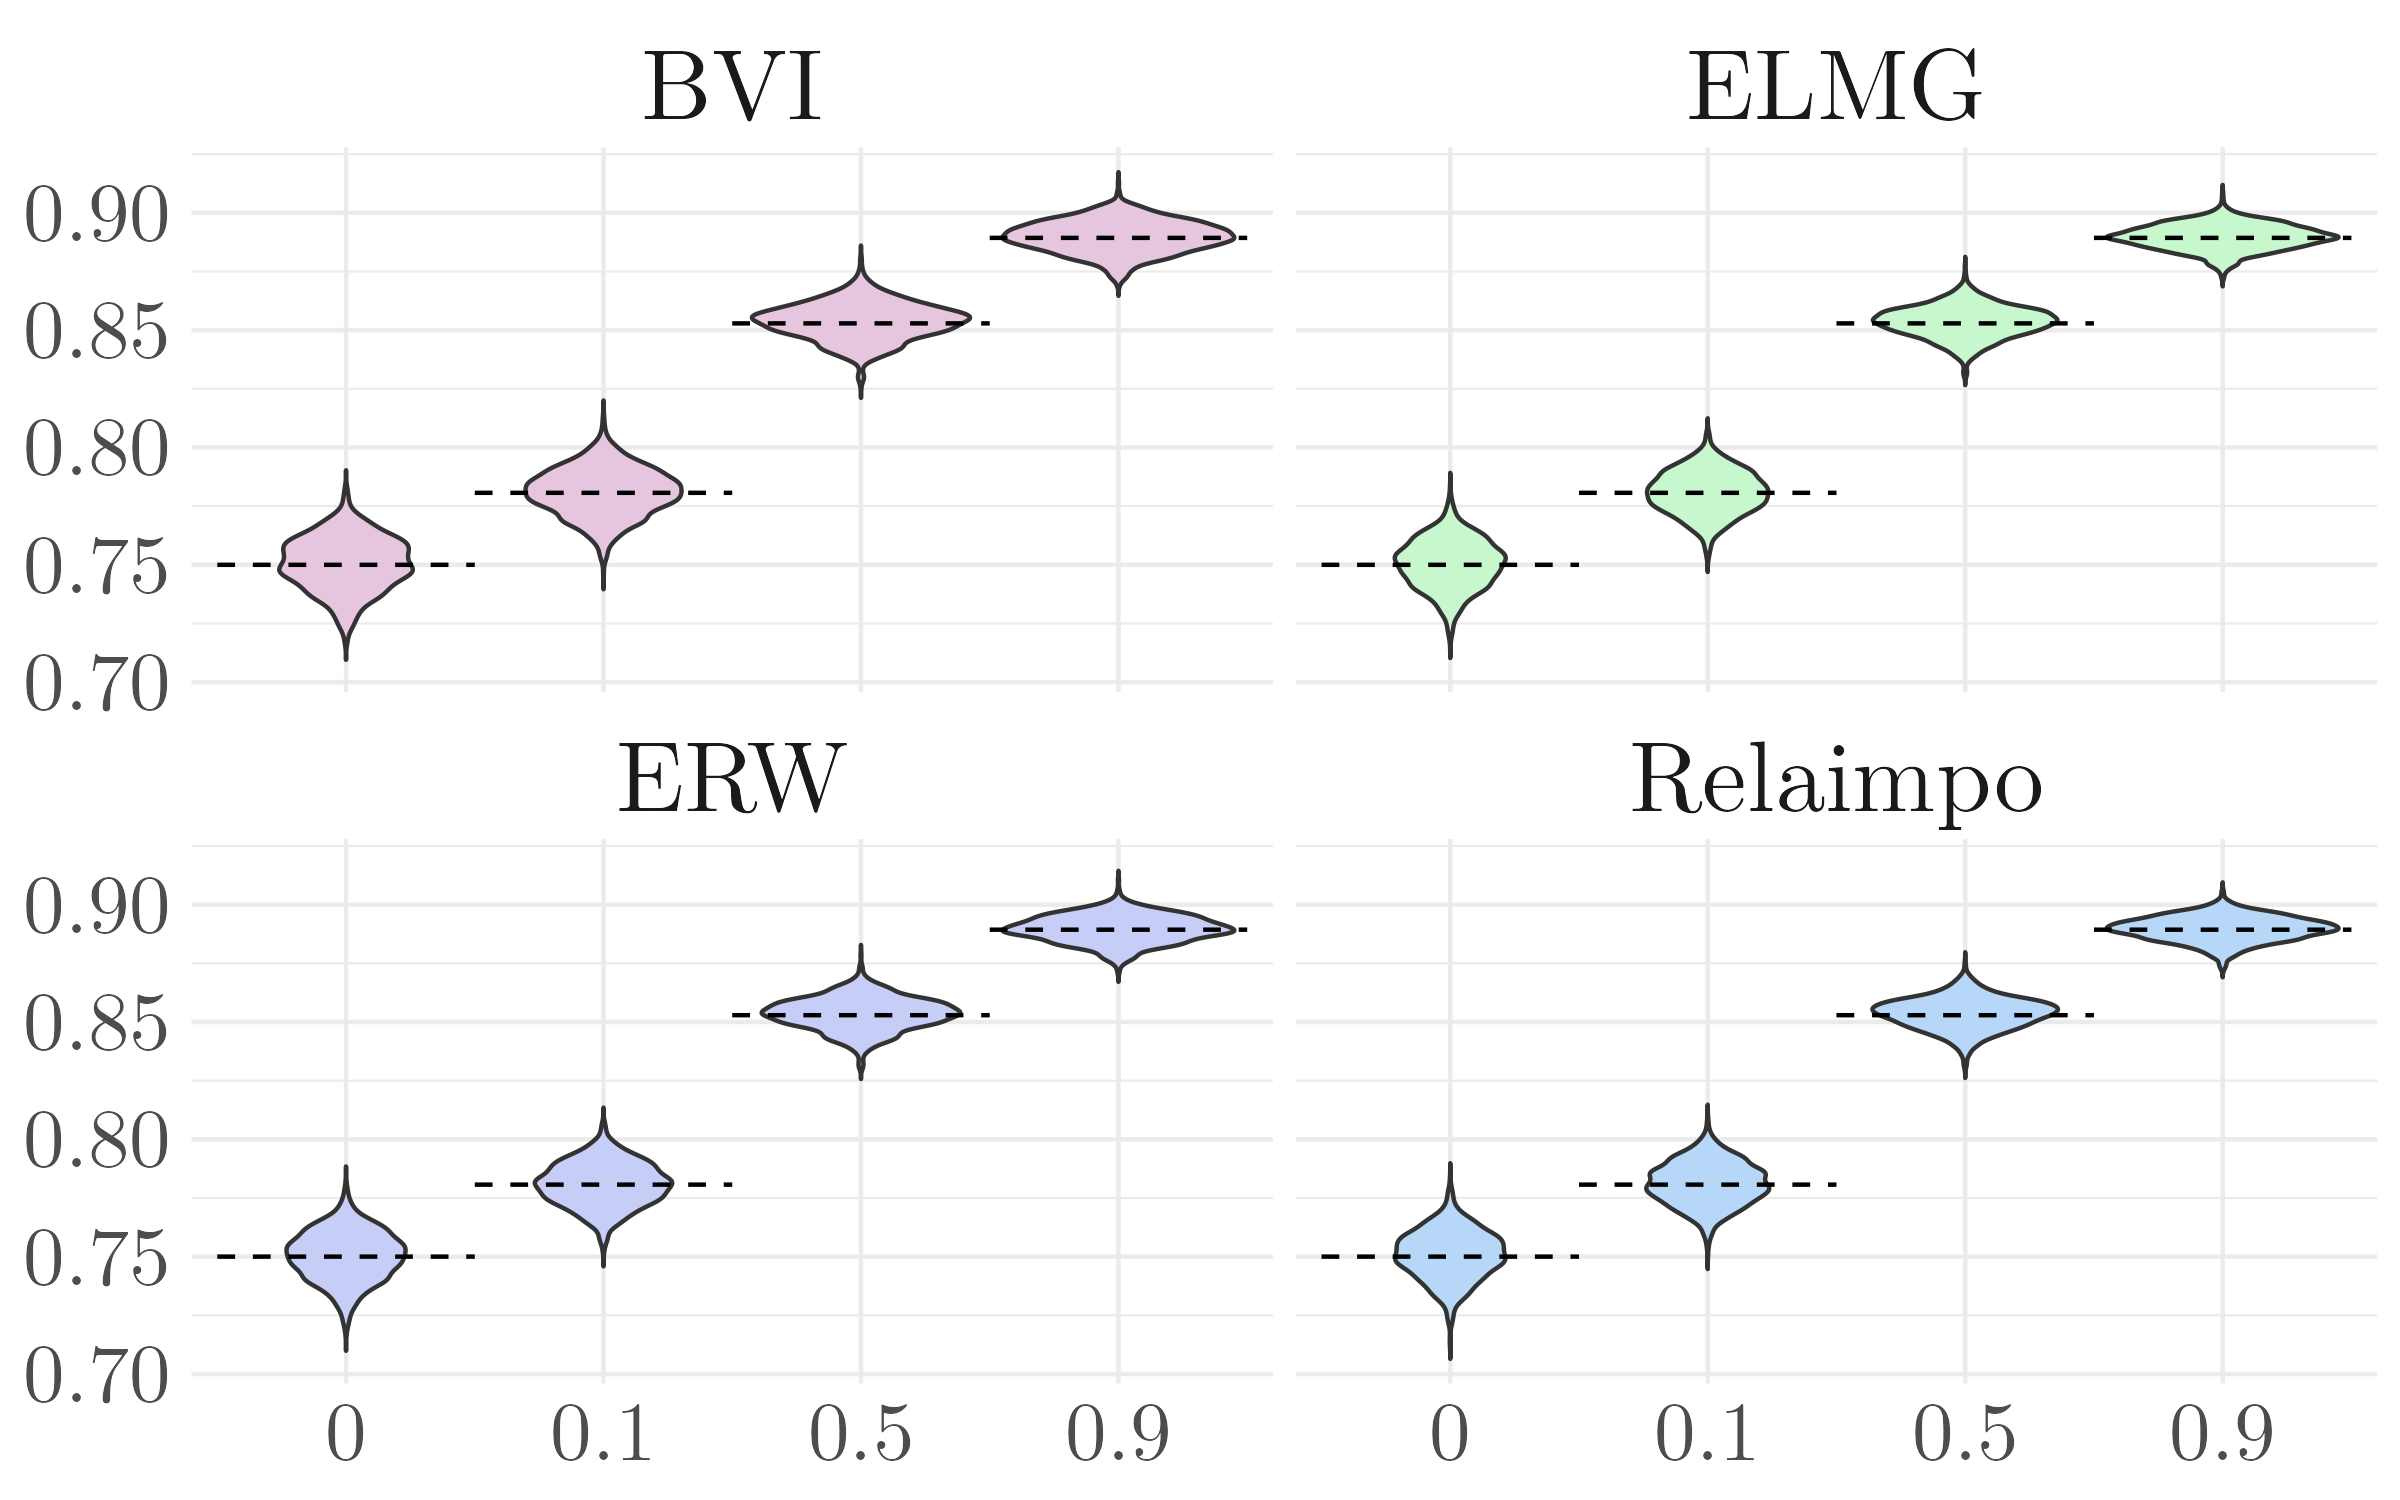
\includegraphics[width=0.55\linewidth]{Figures/ViolinPlots/Marginal_Variance.png}
    \label{fig:variance_marginal}
  }
  \hfill
  \subfloat{
    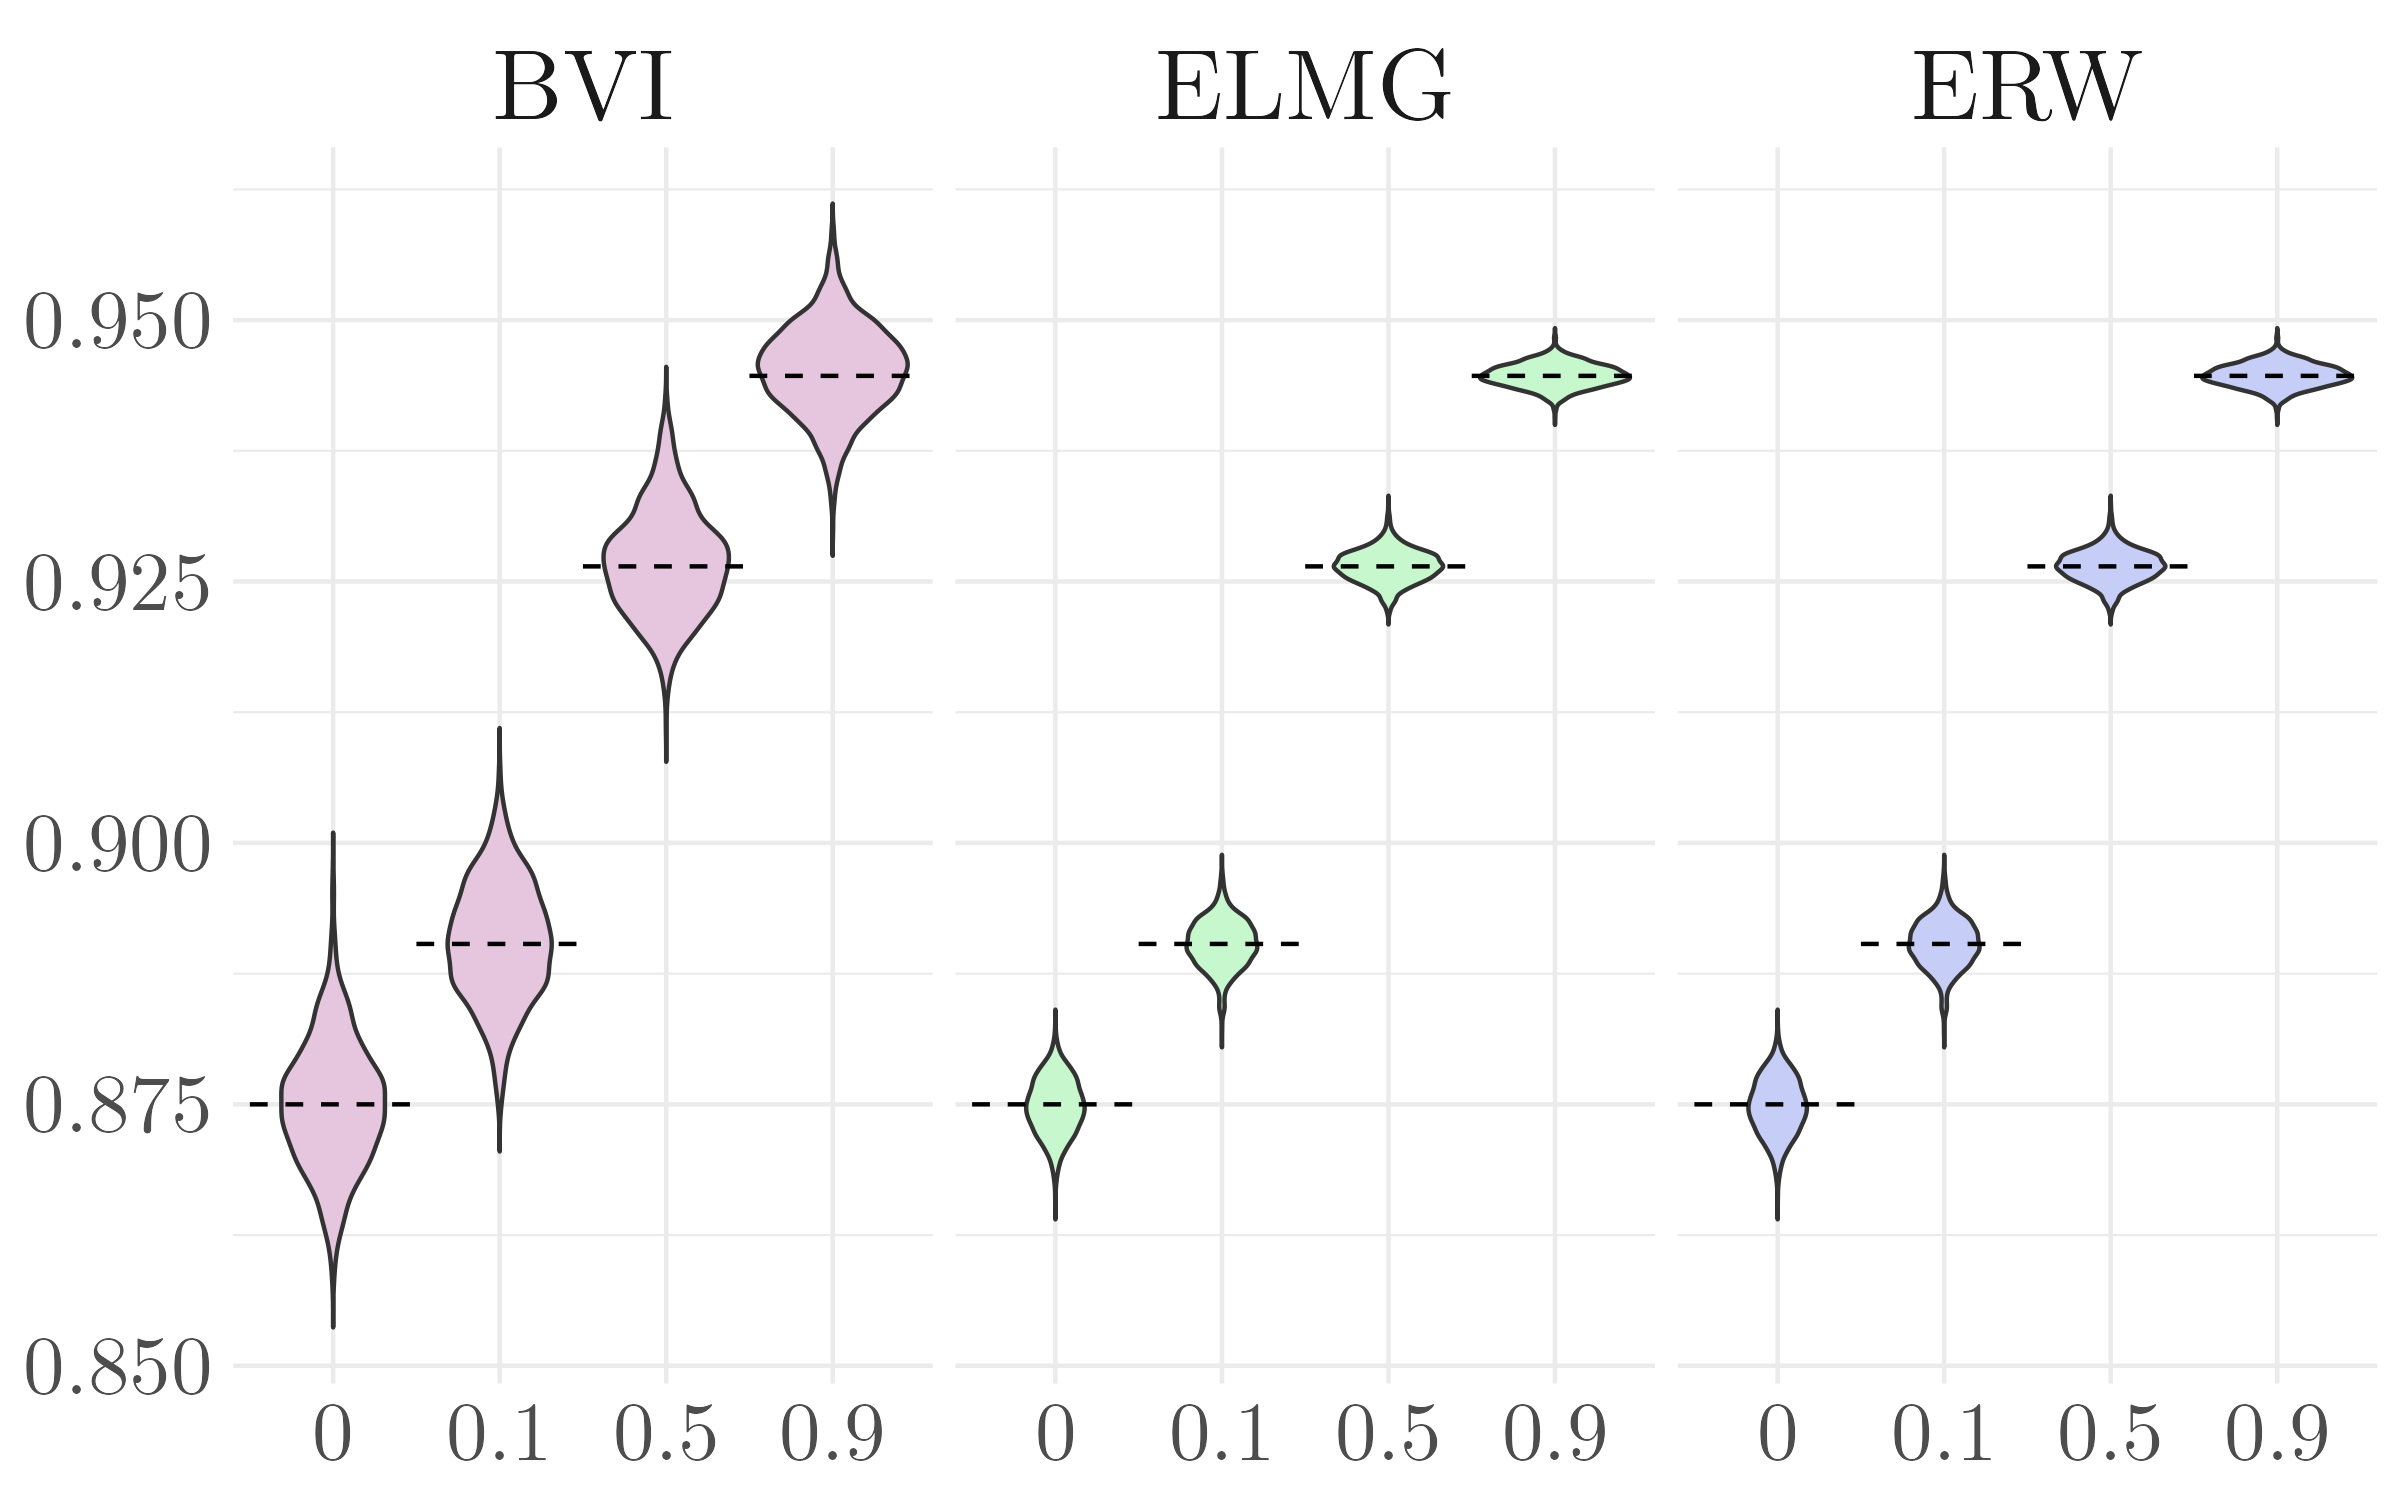
\includegraphics[width=0.55\linewidth]{Figures/ViolinPlots/Conditional_Variance.png}
    \label{fig:variance_conditional}
  }
  \caption[Marginal and conditional $R^2$ in Gaussian LMM]{Violin plots for the total marginal (top) and conditional (bottom) variance explained ($R^2$) for different correlation levels displayed along the x-axis, calculated from the ensemble of simulated datasets by the BVI, ELMG, the ERW and the Relaimpo method(only marginal variance explained can be computed). For the BVI method the posterior means of the sampled posterior distributions of $\boldsymbol{\beta}$ and the marginal distribution of $\hat{\sigma}^2_{\alpha}$ in each simulation are used to compare to the point estimates of the other two methods. The horizontal lines display the theoretical explained variance for each correlation level $\rho$ as in \Cref{table:2}.}
  \label{fig:total_variance}
\end{figure}

\section{Modelling house sparrow traits}
\label{sec:heritability_results}
We now investigate the results of applying our method to the house sparrow dataset. The presented results contain the sampled relative importance distributions of all covariates used to model body mass, wing length and tarsus length. A particular analysis is done on the heritability, as this is a special case of relative importance (\Cref{sec:heritability}) and is the focus of much research. However, our method also enables a more comprehensive analysis by providing the relative variable importance of all covariates. The samples of heritability are sampled from the variance component that captures additive genetic variance (\textit{IDC2}), and we use the results from \citet{Silva2017} and \citet{Muff2019Genetic} for comparison. For this analysis, the covariance structure of the pedigree required us to model more complex random effects than i.i.d. random intercepts, and so the \texttt{rptR} package could not be used for comparisons. In \Cref{table:summary_heritability} the mean of sampled heritability along with quantile values is presented, as well as the corresponding measures from the comparable studies.
% \begin{table}[H]
%   \centering
%   \begin{tabular}{lccccccc}
%   \toprule
%    & \multicolumn{2}{c}{\citet{Silva2017}} & \multicolumn{2}{c}{\citet{Muff2019Genetic}} & \multicolumn{2}{c}{BVI} \\ 
%    \cmidrule(lr){2-3} \cmidrule(lr){4-5} \cmidrule(lr){6-7}
%    & Estimate & CI & Estimate & CI & Mean & CI \\ 
%   \midrule
%   $h^2_{\text{mass}}$    & 0.300 & [0.231, 0.369] & 0.288 & [0.219, 0.371] & 0.283 & [0.232, 0.344] \\
%   $h^2_{\text{wing}}$    & 0.388 & [0.353, 0.461] & 0.344 & [0.294, 0.409] & 0.356 & [0.322, 0.393] \\
%   $h^2_{\text{tarsus}}$  & 0.415 & [0.333, 0.497] & - & - & 0.401 & [0.330, 0.470] \\ 
%   \bottomrule
%   \end{tabular}
%   \caption[Heritability estimates and confidence intervals]{Heritability estimates and confidence interval from \citet{Silva2017}, posterior means of additive genetic variance divided by the posterior means of total phenotypic variance in \citet{Muff2019Genetic} with corresponding confidence interval and the mean and confidence interval of the heritability samples obtained from the BVI method for the phenotypic traits; body mass, wing length and tarsus length.}
%   \label{table:summary_heritability}
% \end{table}
\begin{table}[H]
  \centering
  \small
  \begin{tabular}{lccccccc}
    \toprule
    & \multicolumn{2}{c}{$h^2_{\text{mass}}$} & \multicolumn{2}{c}{$h^2_{\text{wing}}$} & \multicolumn{2}{c}{$h^2_{\text{tarsus}}$} \\
    \cmidrule(lr){2-3} \cmidrule(lr){4-5} \cmidrule(lr){6-7}
    & Est. & CI & Est. & CI & Est. & CI \\
    \midrule
    \citet{Silva2017} & 0.300 & [0.231, 0.369] & 0.388 & [0.353, 0.461] & 0.415 & [0.333, 0.497] \\
    \citet{Muff2019Genetic} & 0.288 & [0.219, 0.371] & 0.344 & [0.294, 0.409] & - & - \\
    %BVI grid & 0.282 & [0.231, 0.342] & 0.356 & [0.322, 0.393] & 0.401 & [0.329, 0.468] \\
    BVI & 0.284 & [0.255, 0.315] & 0.356 & [0.334, 0.380] & 0.401 & [0.363, 0.438] \\
    \bottomrule
  \end{tabular}
  \caption[Heritability estimates and confidence intervals]{Heritability estimates and confidence intervals from \citet{Silva2017}, posterior means of additive genetic variance divided by the posterior means of total phenotypic variance in \citet{Muff2019Genetic} with corresponding confidence intervals, and the mean and quantile values of the heritability samples obtained from the BVI method for the phenotypic traits: body mass, wing length, and tarsus length. Note that in \citet{Muff2019Genetic} no estimate of tarsus length heritability was provided.}
  \label{table:summary_heritability}
\end{table}
\noindent For the sampled heritability of body mass, we have a mean of $0.284$ and the interval $[0.255, 0.315]$ covers the $95$th percentile (\Cref{table:summary_heritability}). In general, the posterior distribution of heritability has a Gaussian shape, centered around the mean value (\Cref{fig:heritability_mass_combined}). The posterior distribution of relative importance of the fixed effects predominantly shows very small values. Recall that importance calculations of fixed effects include squaring the coefficients, and so no negative importance can be allocated to a covariate. Notably, the relative importance of covariates \textit{FGRM} and \textit{other} exhibits a negative exponential decay pattern, while the covariates \textit{sex, age} and \textit{outer} seem to have a skewed normal distribution. The posterior distribution of relative importance allocated to \textit{month} looks normally distributed. Considering the random effects, it is evident that they have been allocated a much larger share of importance compared to the fixed effects. The importance of the Gaussian observations have a normal shape and are often allocated over $50\%$ of the total importance. The distribution of importance for \textit{IDC} does not seem to follow any standard distribution, which is the covariate accounting for individual differences. Lastly, \textit{hatchyear} is allocated a quite small importance, and the distribution looks like a skewed normal distribution. To fit the model and obtain the samples, the BVI method took about $73$ seconds. Overall, the heritability values for body mass are in close agreement with the estimates from \citet{Silva2017} and \citet{Muff2019Genetic}, and the posterior importance distributions for all covariates seem to be reasonable. 
\begin{figure}[H]
  \centering
  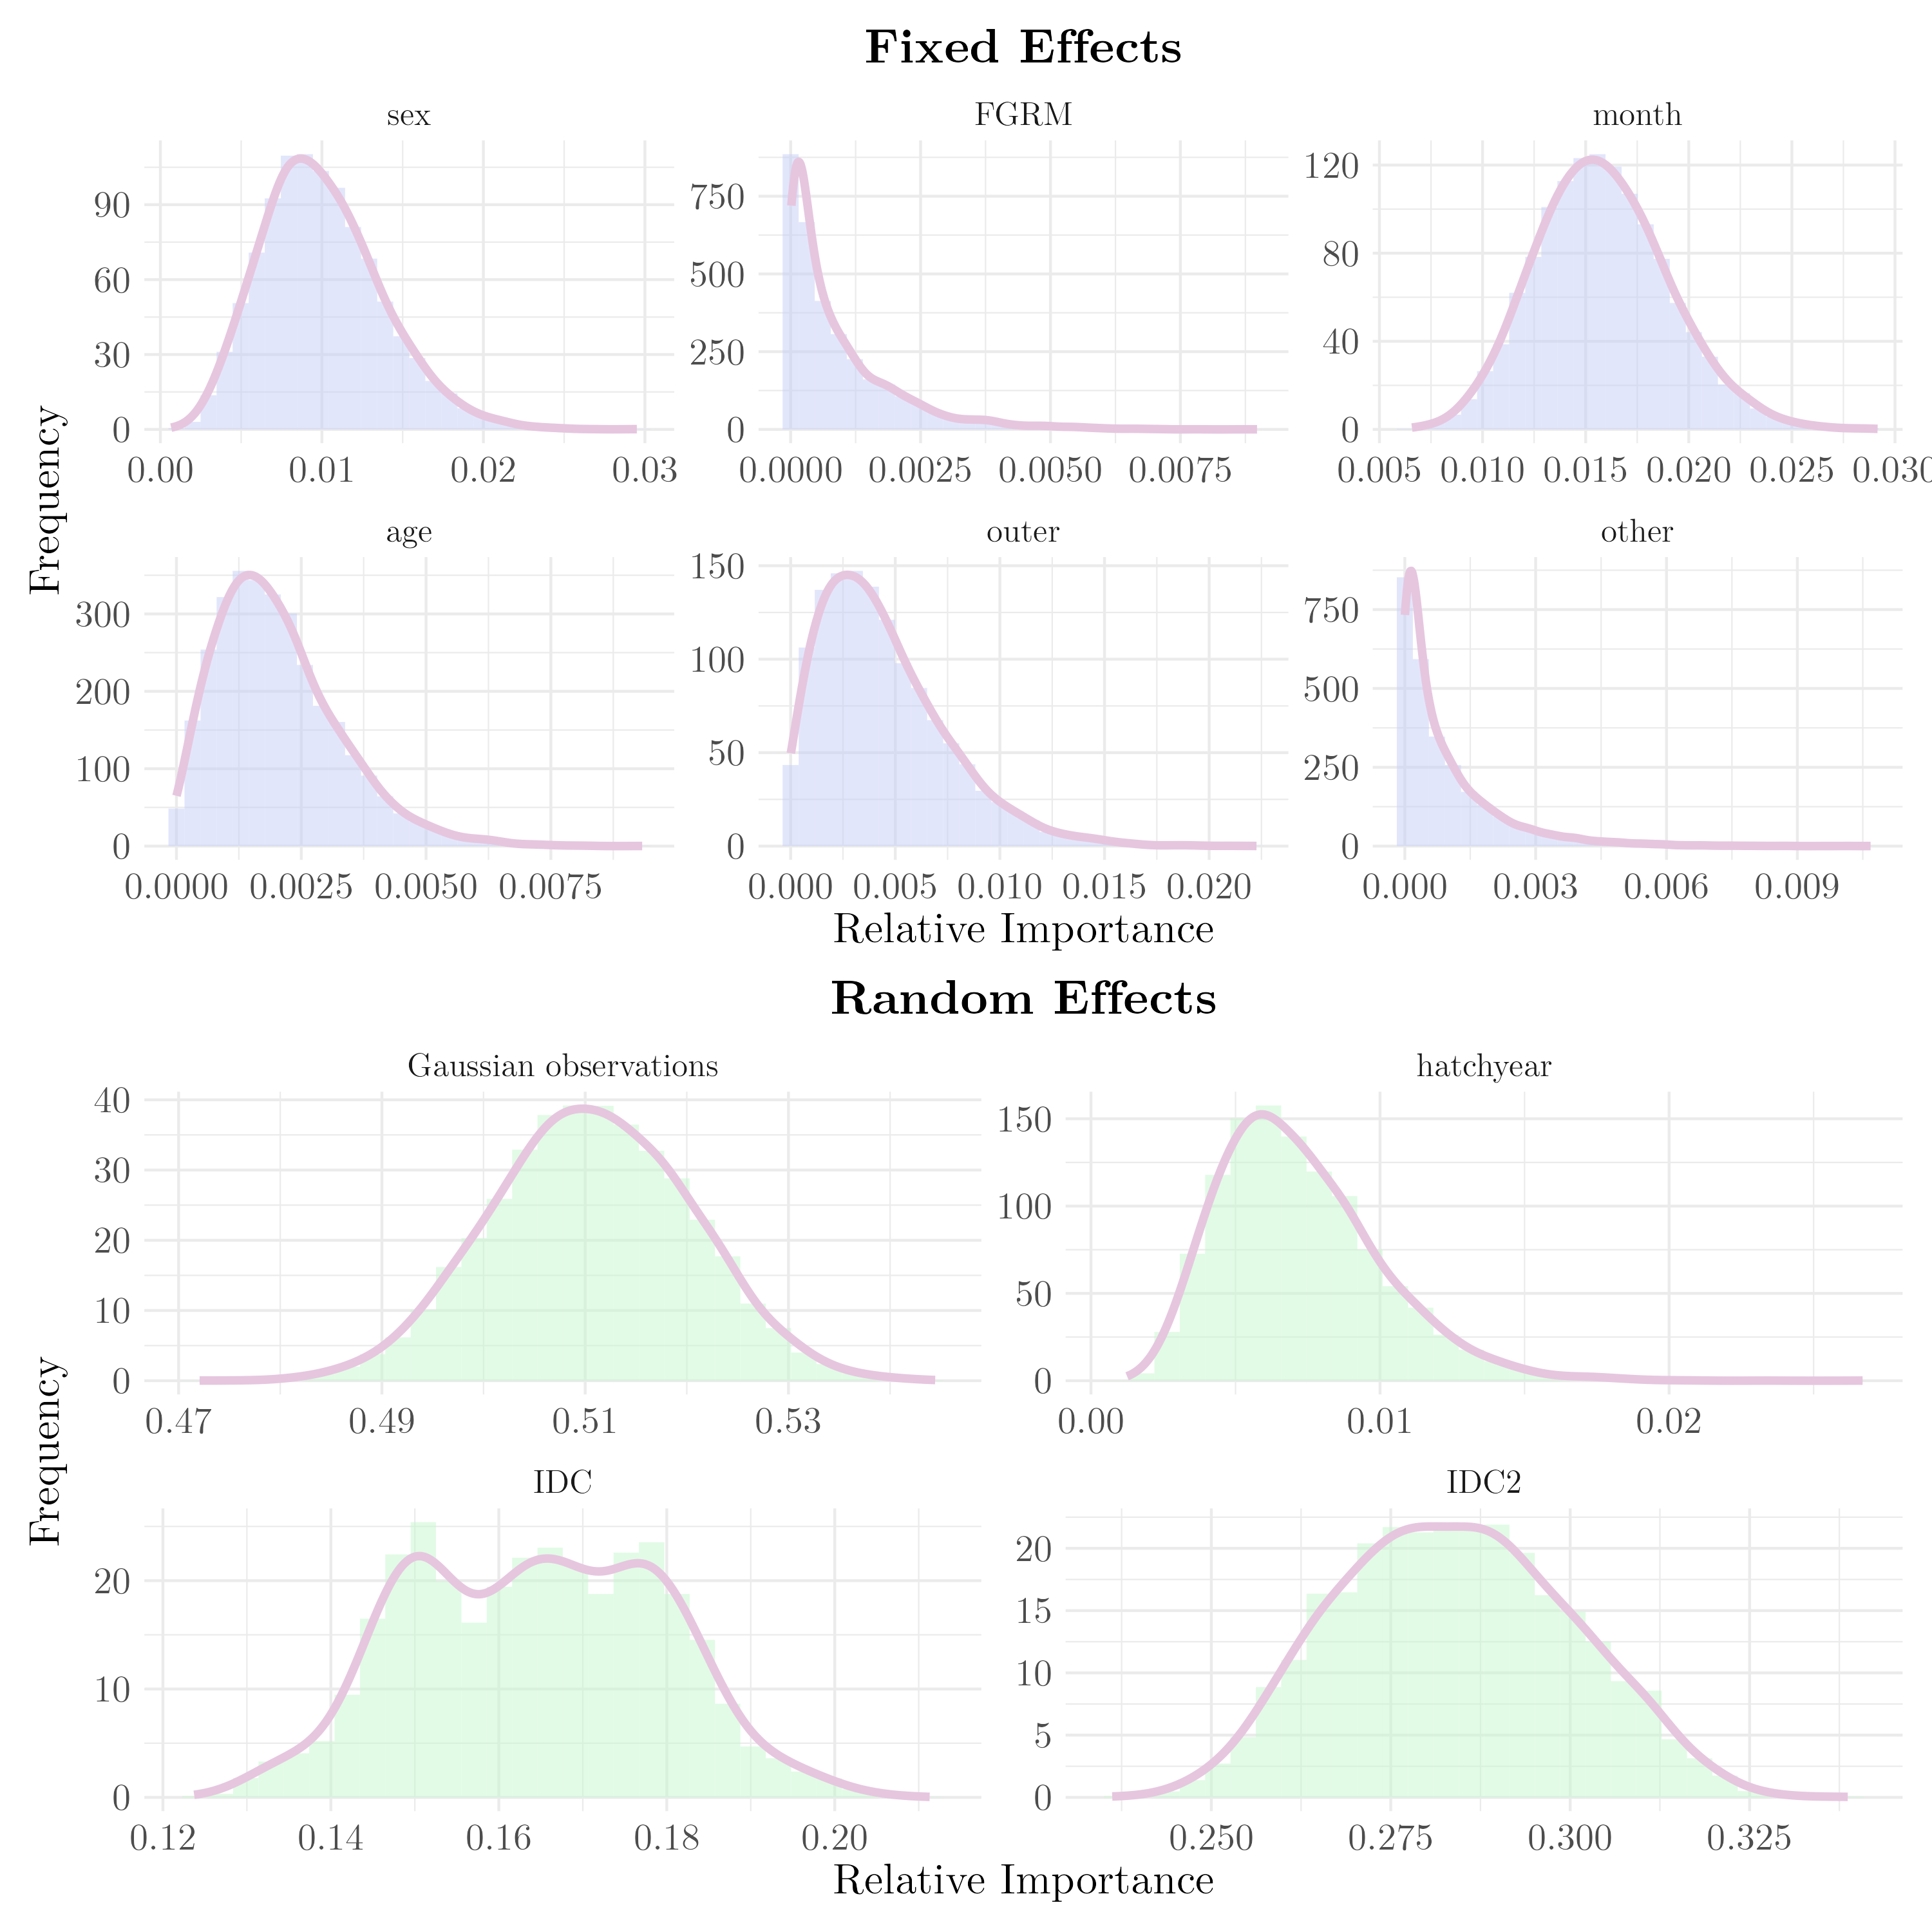
\includegraphics[width=1\linewidth]{Figures/House sparrow study/Mass_ccd.png}
  \caption[Estimated posterior importance of all covariates in the body mass model from the BVI method]{Histogram depicting the sampled posterior importance values of all covariates used to model body mass by the BVI method for the house sparrow dataset. The heritability estimates correspond to the random effect \textit{IDC2}, and the estimates from the BVI method, \citet{Silva2017} and \citet{Muff2019Genetic} of heritability are found in \Cref{table:summary_heritability}.}
  \label{fig:heritability_mass_combined}
\end{figure}
% \begin{figure}[H]
%   \centering
%   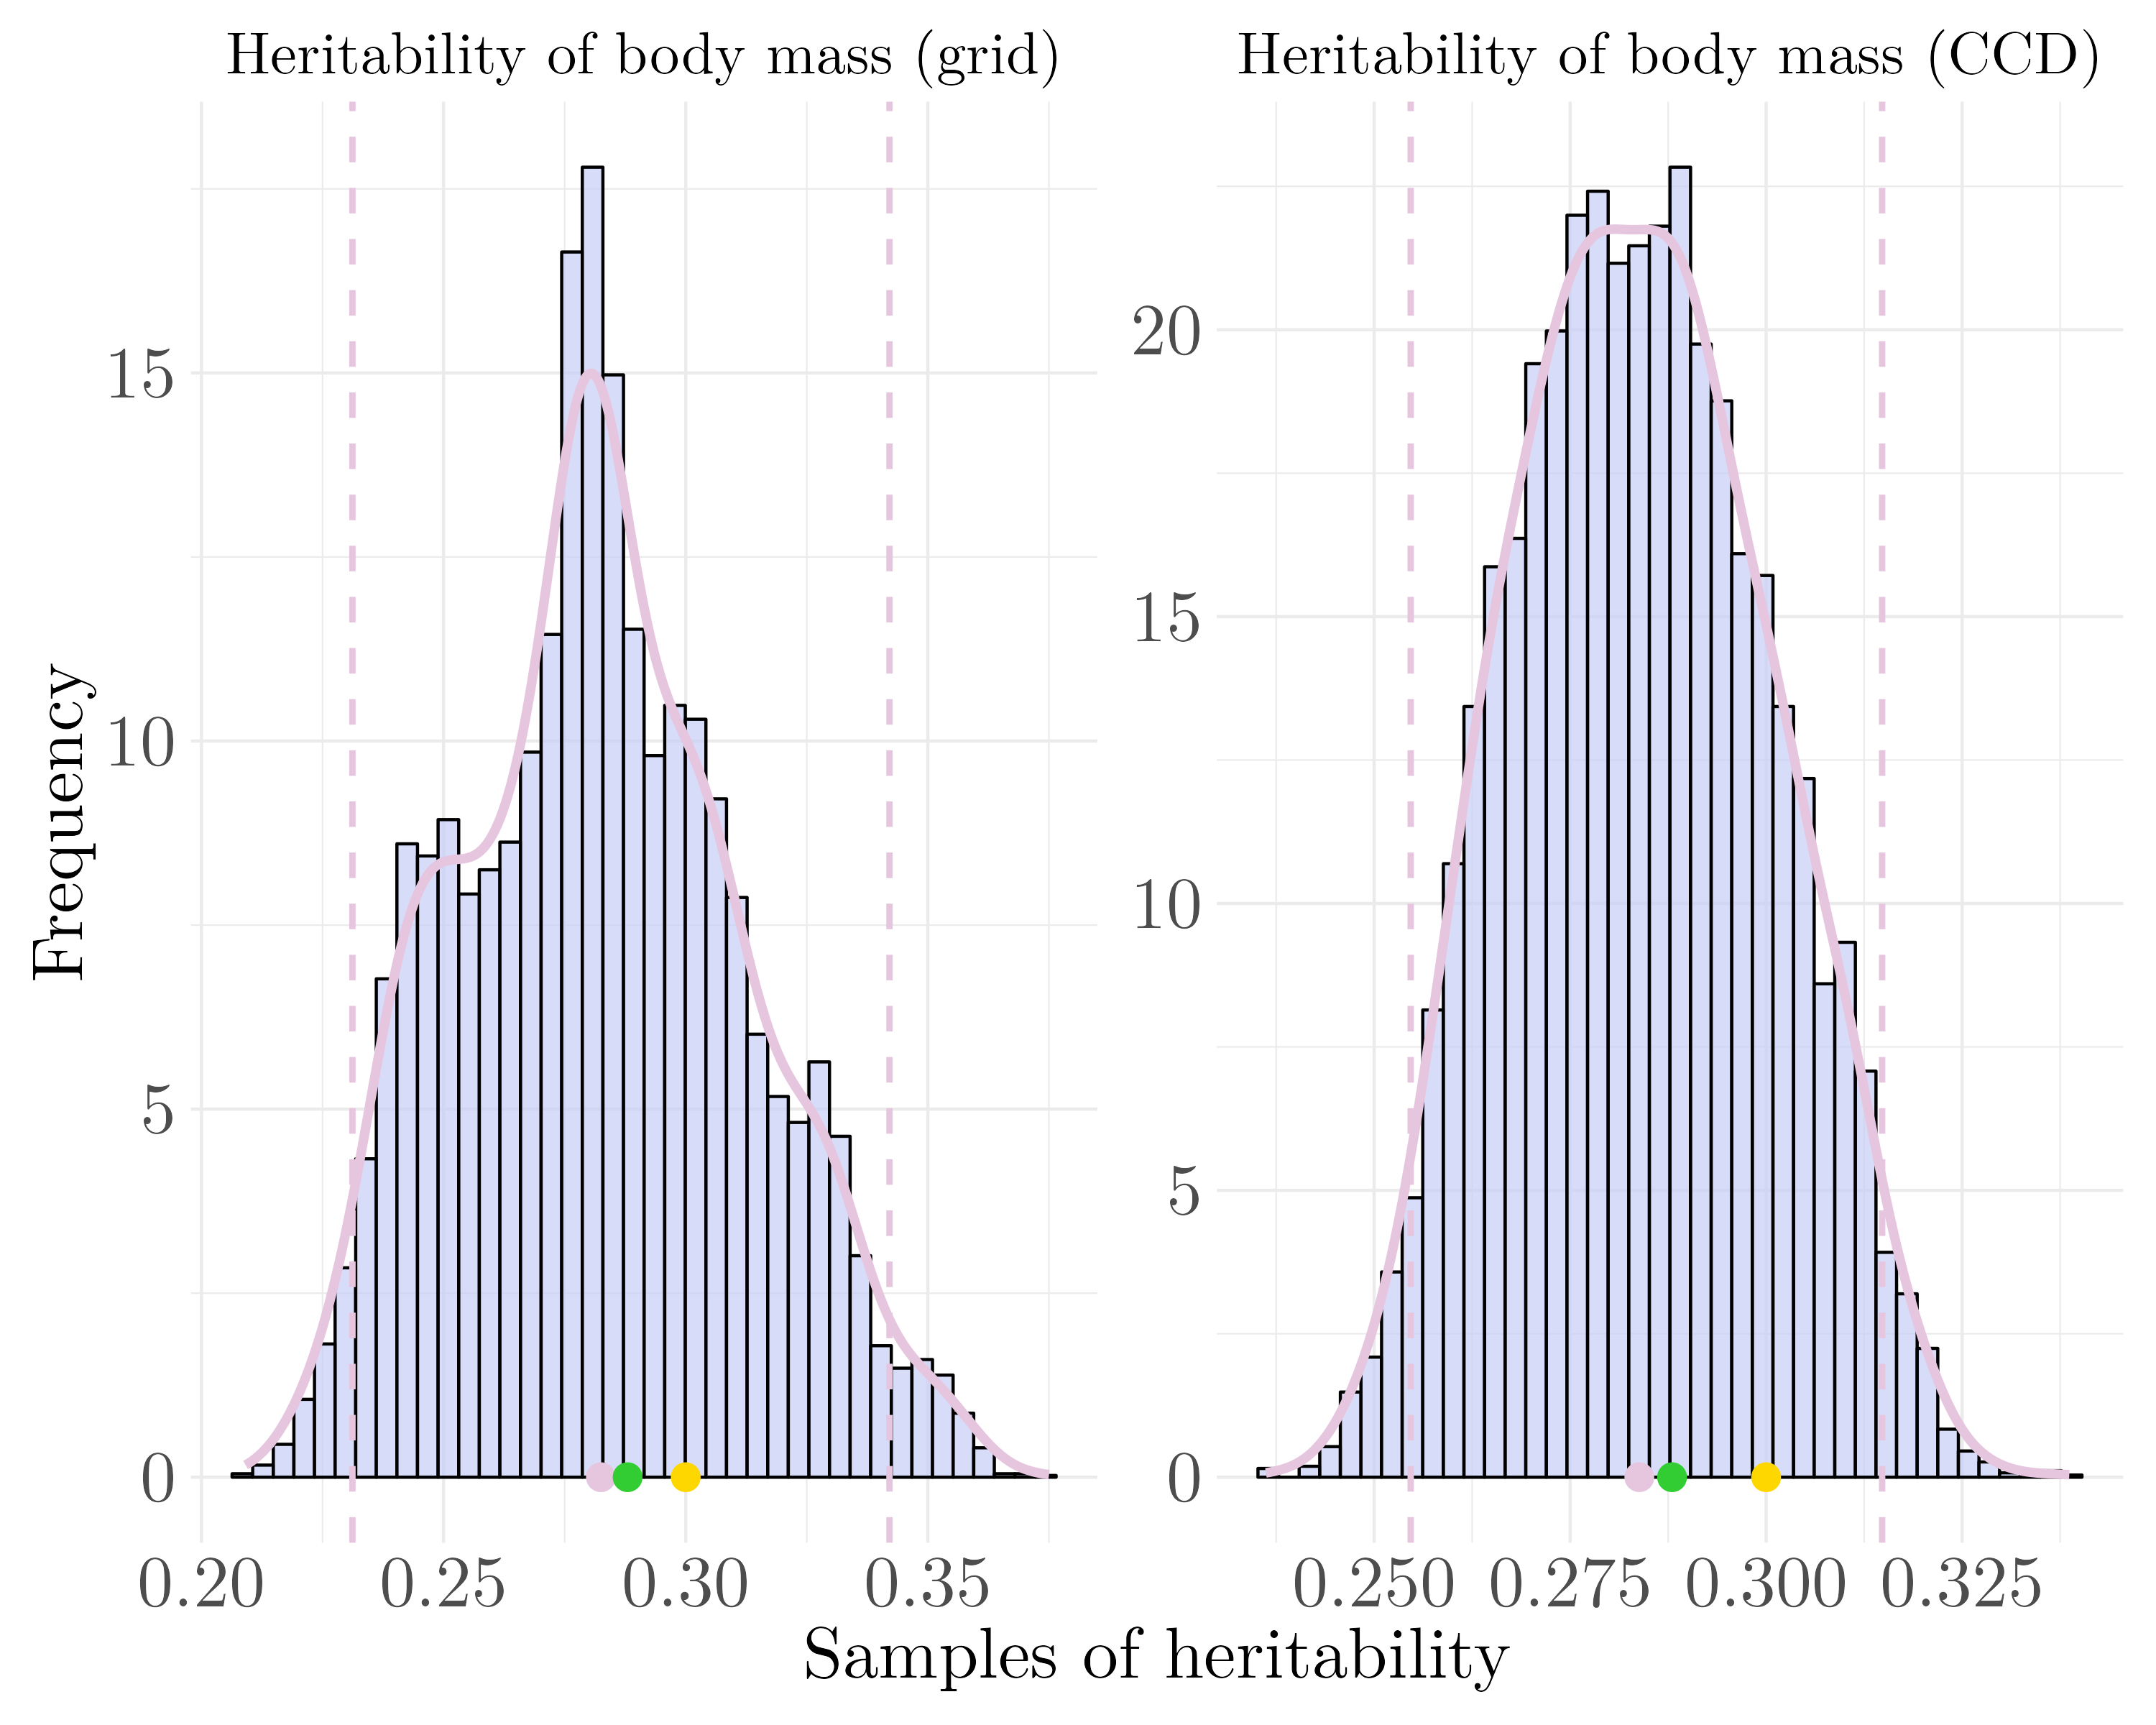
\includegraphics[width=1\linewidth]{Figures/House sparrow study/Heritability_mass_combined.png}
%   \caption[Estimated heritability of body mass from grid and CCD strategy]{Histogram depicting the estimated heritability values of body mass by the BVI method for the grid integration strategy(left) and CCD integration strategy (right) for the house sparrow dataset. The mean of the samples is marked as a pink circle at the bottom of the histogram, with the lower and upper value for the $95\%$ percentile marked as dashed lines. The heritability estimate from \citet{Silva2017} and \citet{Muff2019Genetic} are marked as gold and green dots respectively at the bottom of the histogram.}
%   \label{fig:heritability_mass_combined}
% \end{figure}
\noindent The samples of wing length heritability form a symmetric bell curve, around the mean of $0.356$ (\Cref{fig:heritability_wing_combined} and \Cref{table:summary_heritability}). Further, the $95$th percentile is roughly the interval $[0.334, 0.380]$, which is more narrow than the quantile for the heritability of body mass. Contrary to what was the case for body mass, when modelling wing length, some fixed effects are allocated a significant share of importance. For instance, the distribution of relative importance for \textit{sex} and \textit{age} are centered around $0.340$ and $0.055$ respectively, while the others are allocated an importance of the same order of magnitude as for body mass. Again, some fixed covariates exhibit a decay pattern close to zero (\textit{e.g. FGRM} and \textit{age}), and some seem to have a skewed normal shape (\textit{e.g. sex} and \textit{outer}). For the random effects, we notice that the Gaussian observations are normally distributed and allocated roughly $17.5\%$ of the total importance. Again the \textit{hatchyear} effect is allocated a small importance, and the posterior importance distribution for \textit{IDC} is not easily interpretable, but contains smaller estimates than for body mass. For wing length, the BVI method took about $76$ seconds to fit the model and draw the samples. The heritability estimate from the BVI method lies between the estimates of \citet{Silva2017} and \citet{Muff2019Genetic}, and again we find the posterior importance distributions for all covariates to be plausible.
\begin{figure}[H]
  \centering
  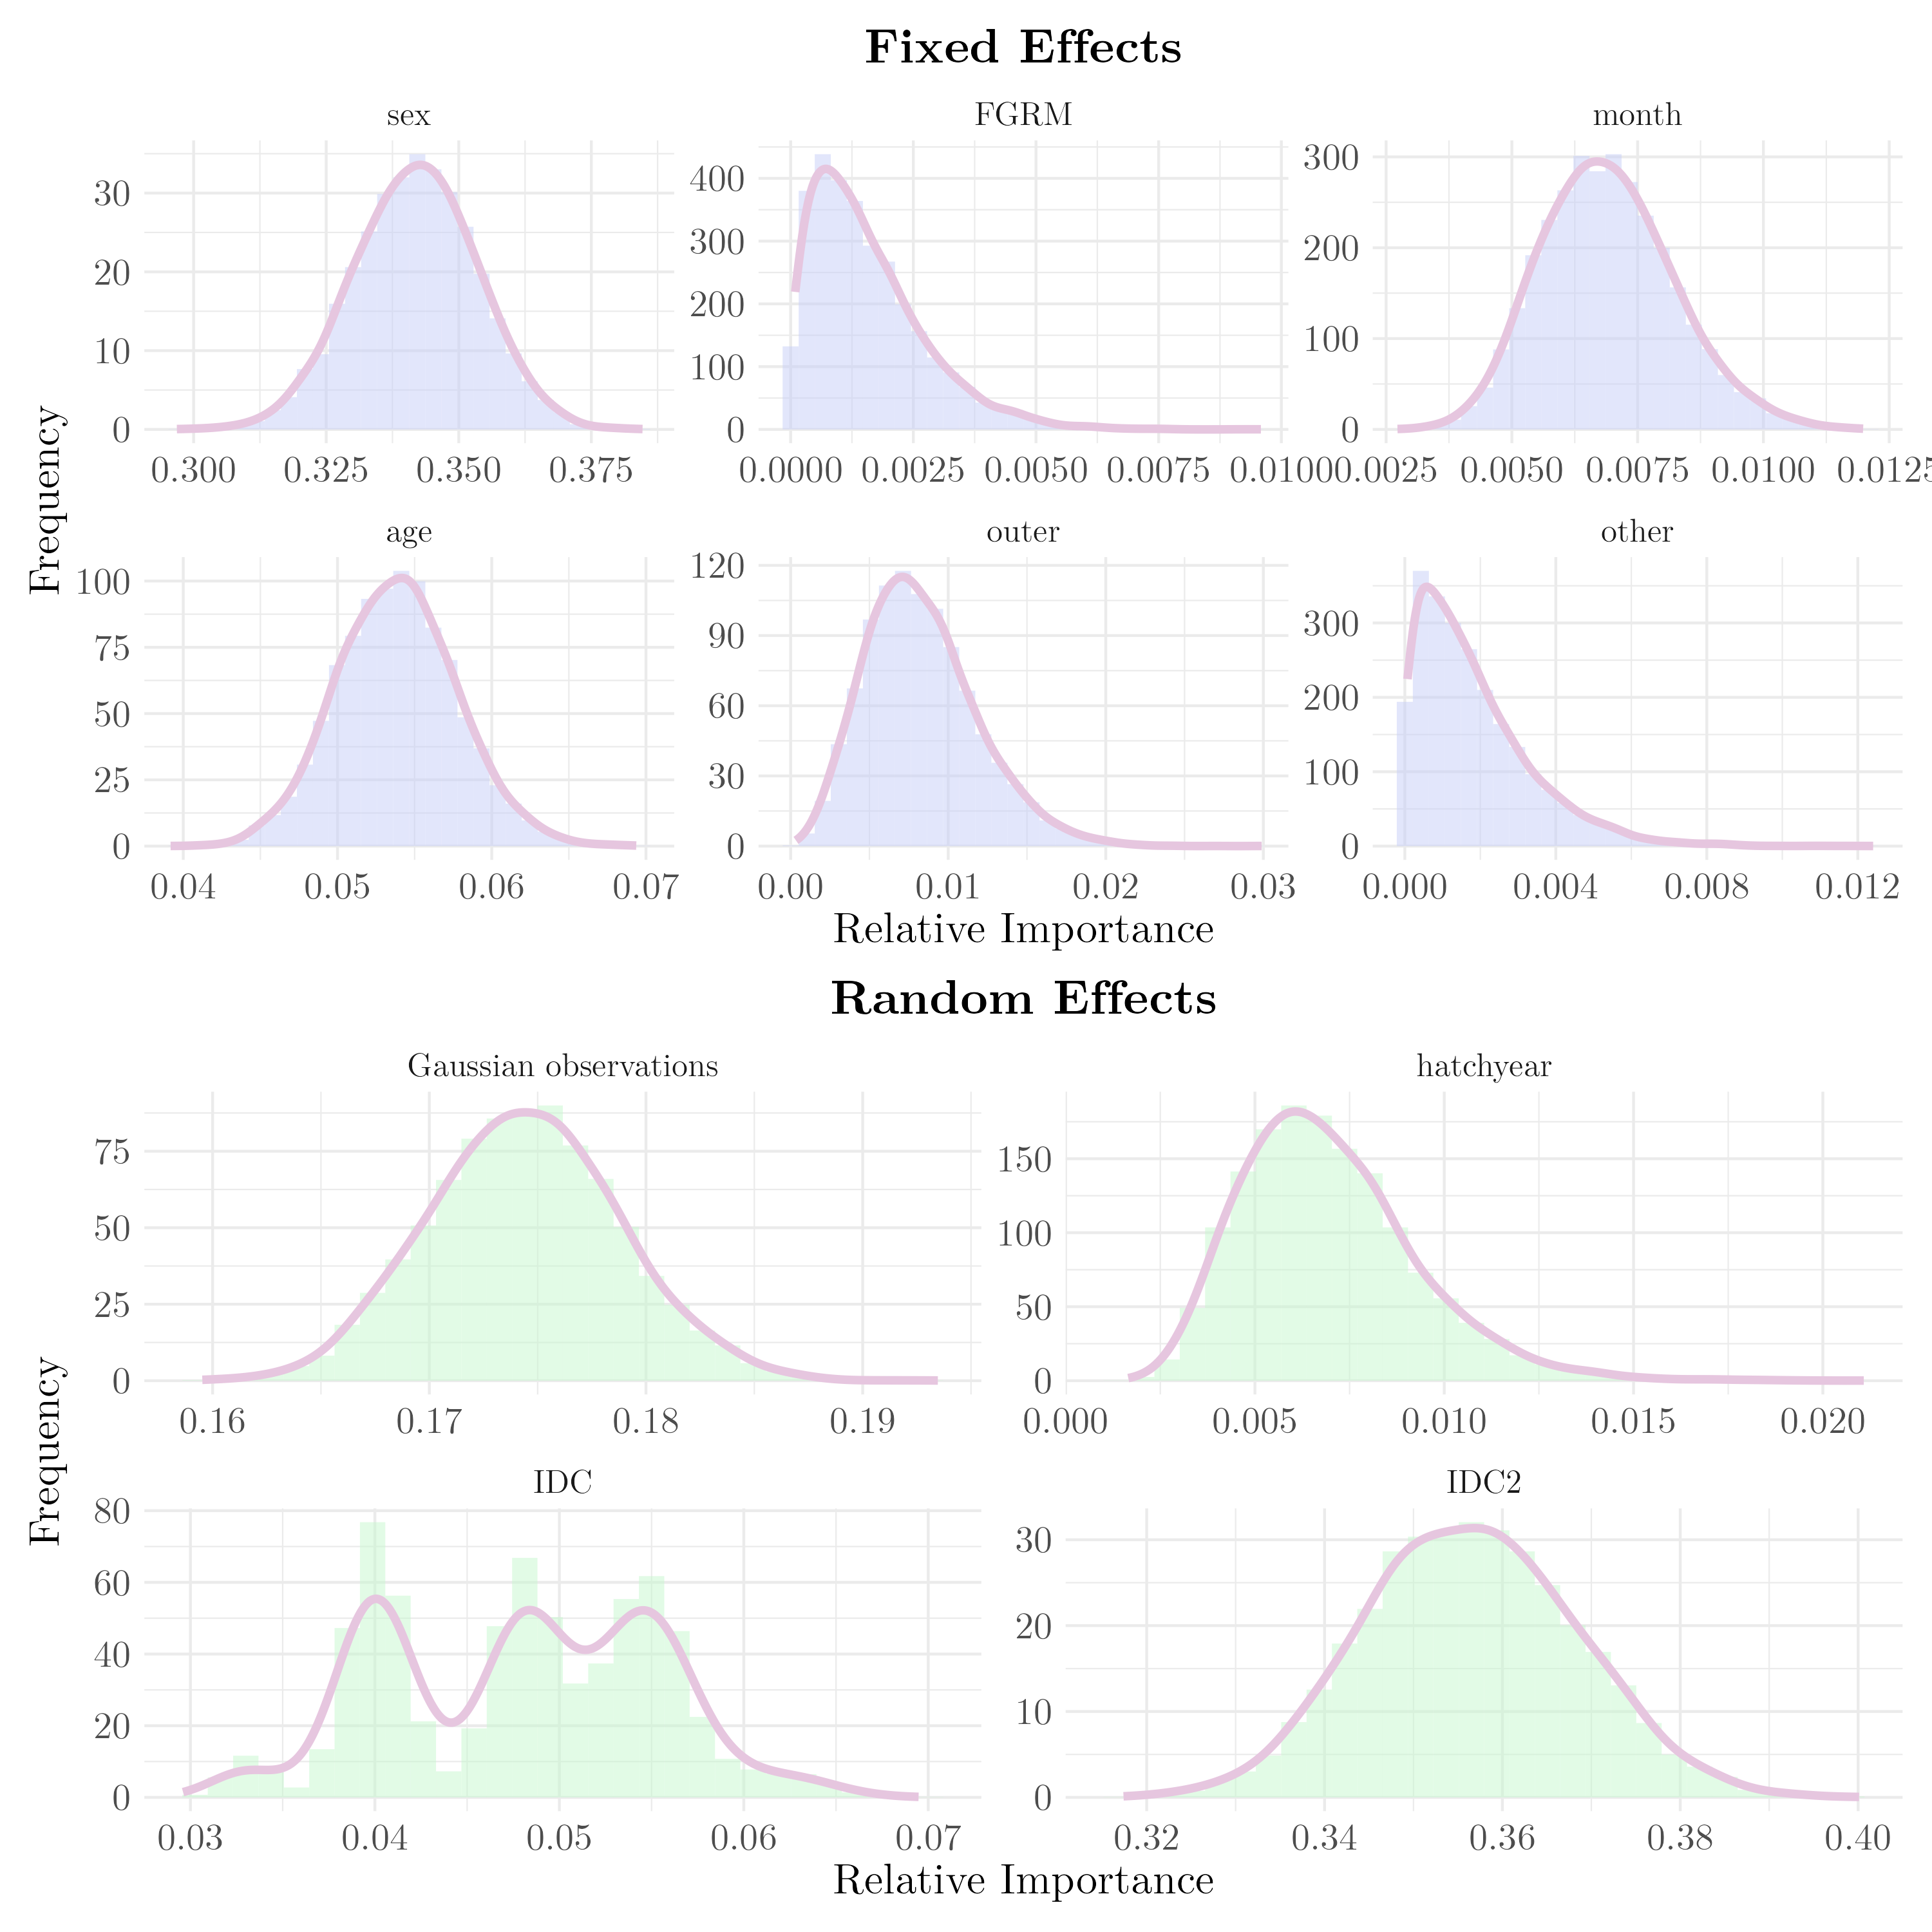
\includegraphics[width=1\linewidth]{Figures/House sparrow study/Wing_ccd.png}
  \caption[Estimated posterior importance of all covariates in the wing length model from the BVI method]{Histogram of the sampled posterior importance values for the covariates modelling wing length from the house sparrows, estimated by the BVI method. The heritability estimates correspond to the random effect \textit{IDC2}, and the estimates from the BVI method, \citet{Silva2017} and \citet{Muff2019Genetic} of heritability are found in \Cref{table:summary_heritability}.}
  \label{fig:heritability_wing_combined}
\end{figure}
% \begin{figure}[H]
%   \centering
%   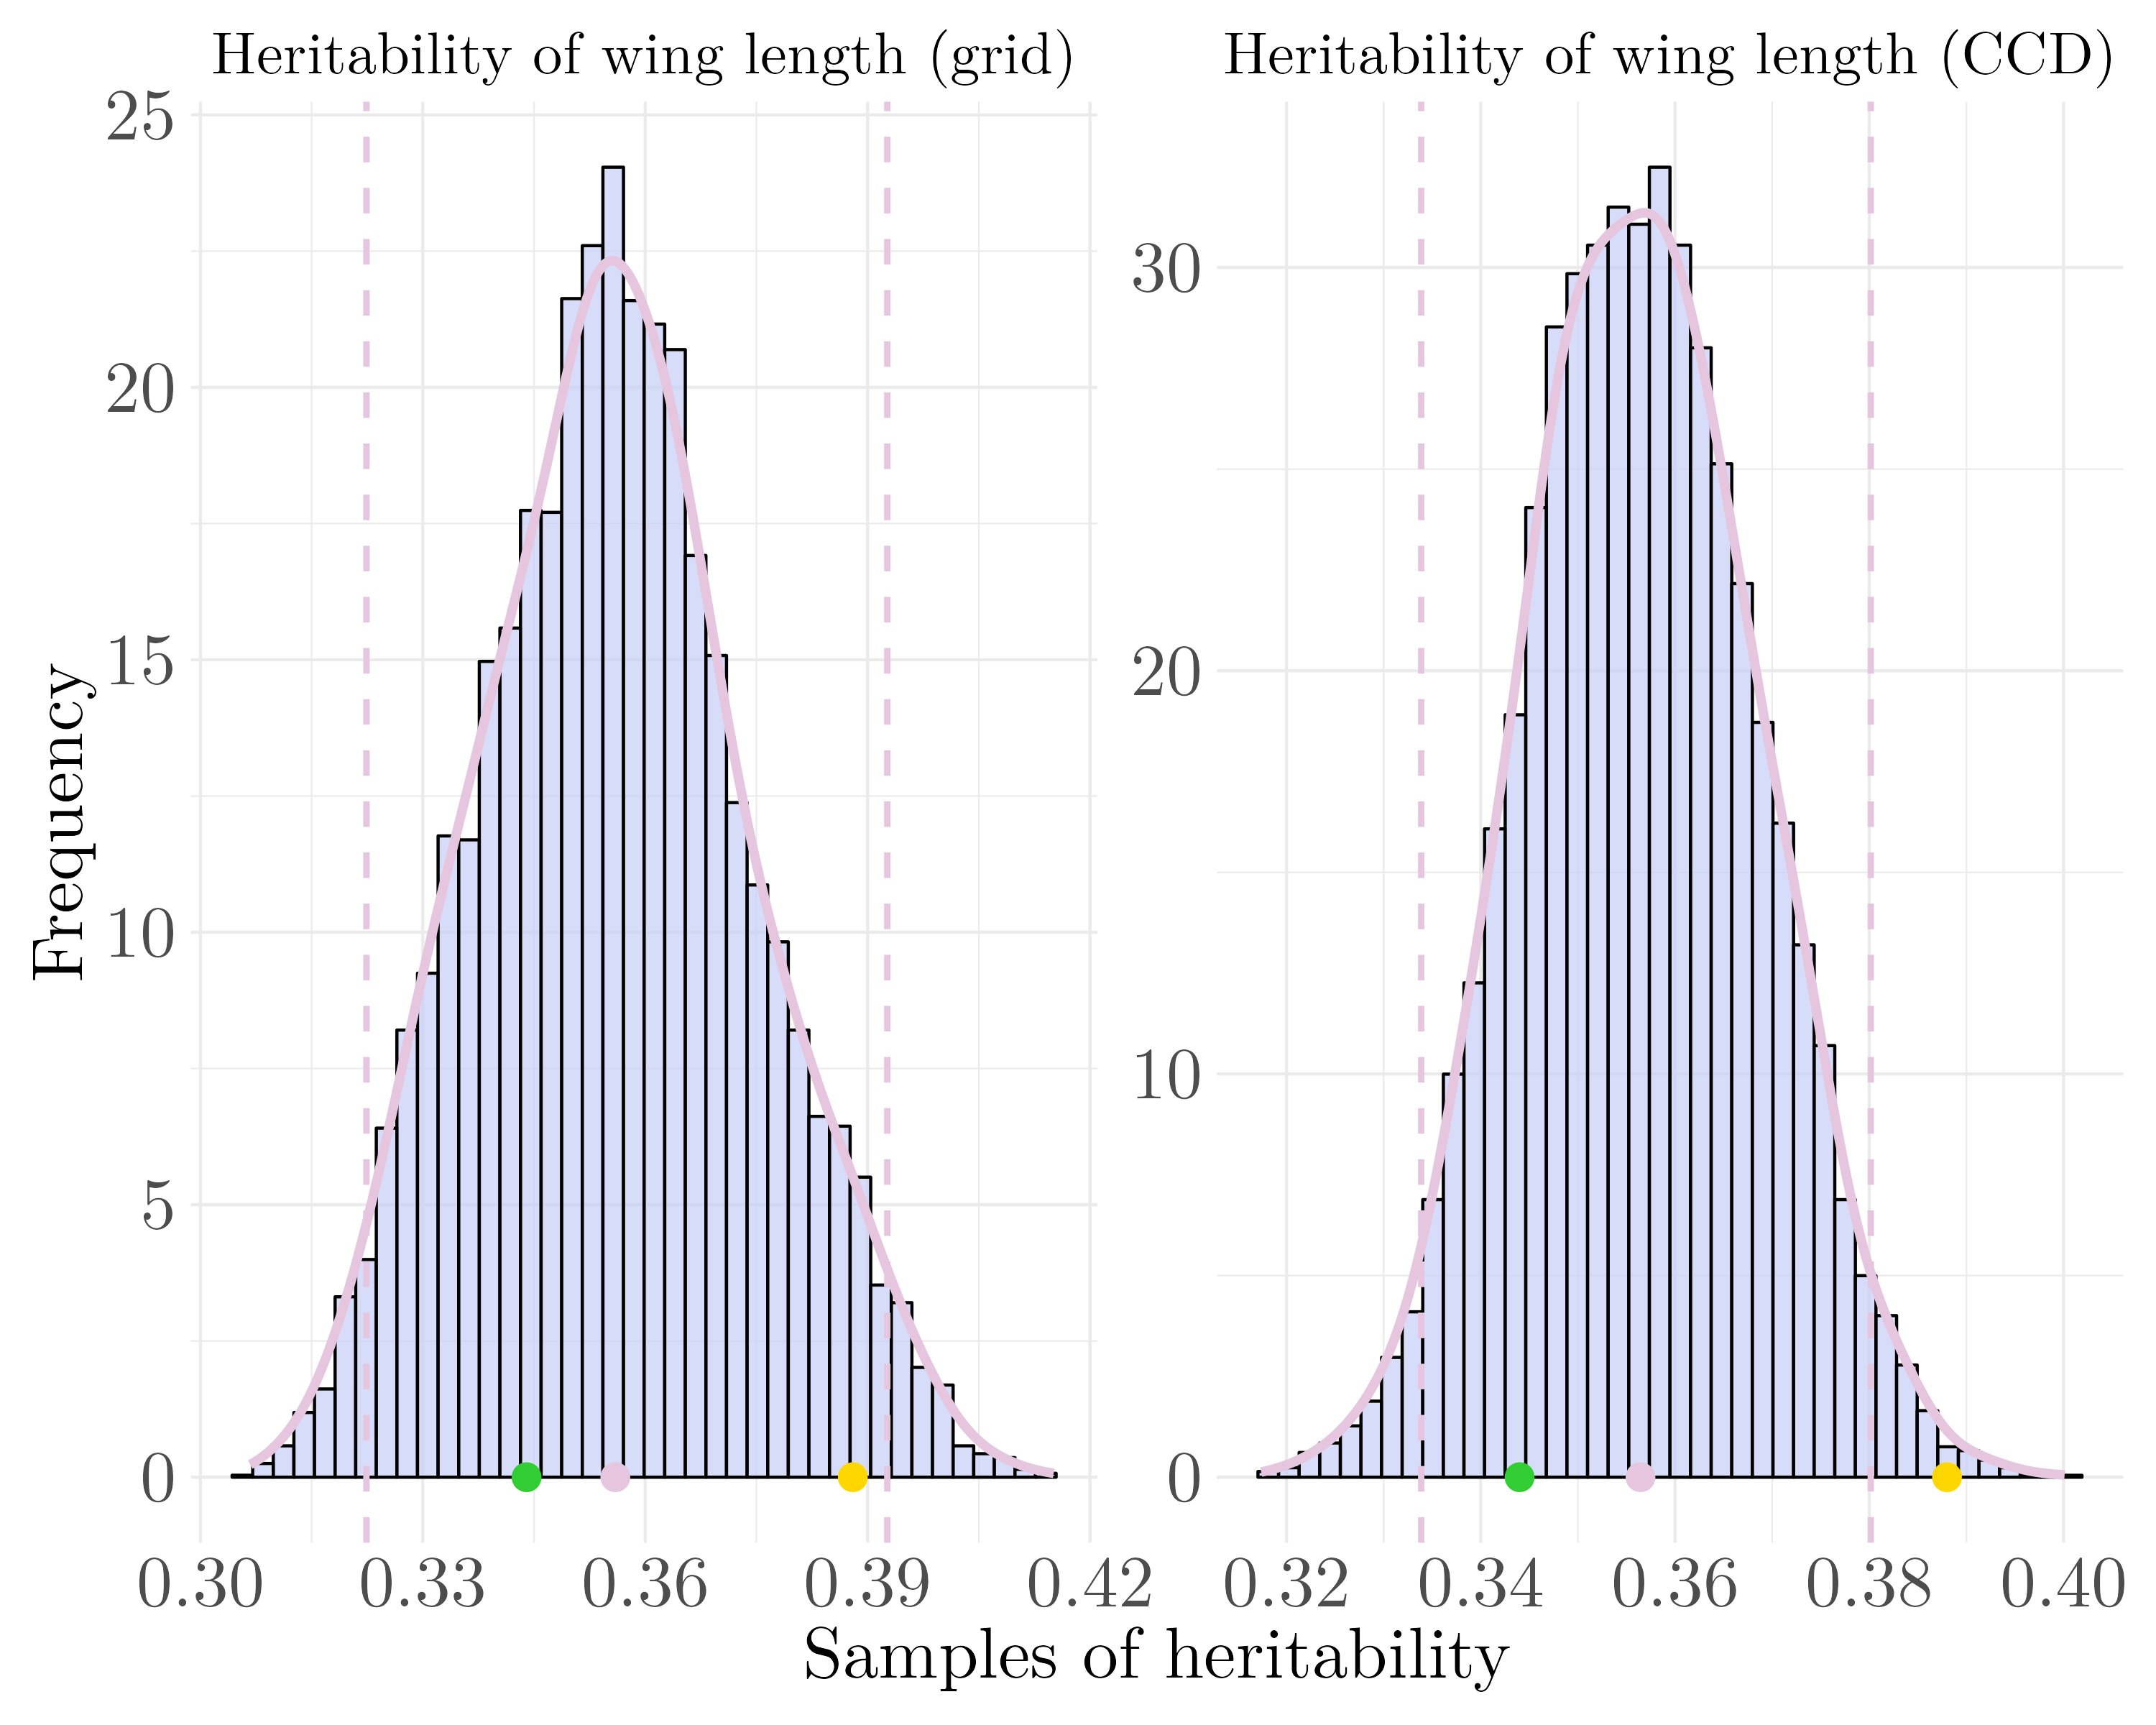
\includegraphics[width=1\linewidth]{Figures/House sparrow study/Heritability_wing_combined.png}
%   \caption[Estimated heritability of wing length]{Histogram of heritability values for wing length of the house sparrows estimated by the BVI method for the grid integration strategy (left) and the CCD integration strategy (right). The mean of the samples is marked as a pink circle at the bottom of the histogram, and the lower and upper value for the $95\%$ percentile are featured as dashed lines. The heritability estimate from \citet{Silva2017} and \citet{Muff2019Genetic} are marked as gold and green dots respectively at the bottom of the histogram.}
%   \label{fig:heritability_wing_combined}
% \end{figure}
\noindent The heritability samples of tarsus length has a mean of $0.401$ and the estimated $95$th quantile is $[0.363, 0.438]$ (\Cref{table:summary_heritability}). This is the largest quantile for all traits, and the posterior distribution of tarsus length heritability seems normal with a broader and flatter peak than for body mass and wing length (\Cref{fig:heritability_tarsus_combined}). As for the body mass model, the posterior distribution of the relative importance allocated to the fixed covariates used to model tarsus length mainly consist of very low values. Here, a strong decay pattern is observable for \textit{age, outer} and \textit{other}, and a moderate decay for \textit{sex} and \textit{FGRM}. The only fixed covariate that looks to have a normal shape is \textit{month}. Conspicuously, the Gaussian observations are given a small share of importance, with a bell curve centered between $0.031$ and $0.032$. The importance of the random effect \textit{hatchyear} is also for tarsus length very small, and the distribution of importance allocated to \textit{IDC} is now a bell curve with a relatively large mean of around $0.538$. To model tarsus length and draw samples, the BVI reported a runtime of $74$ seconds. No heritability estimate from \citet{Muff2019Genetic} was available, however the estimate from the BVI method is close to that of \citet{Silva2017}. 
The posterior importance distributions for all covariates seem reasonable, but the small importances allocated to the random error (Gaussian observations) should be met with caution. 
\begin{figure}[H]
  \centering
  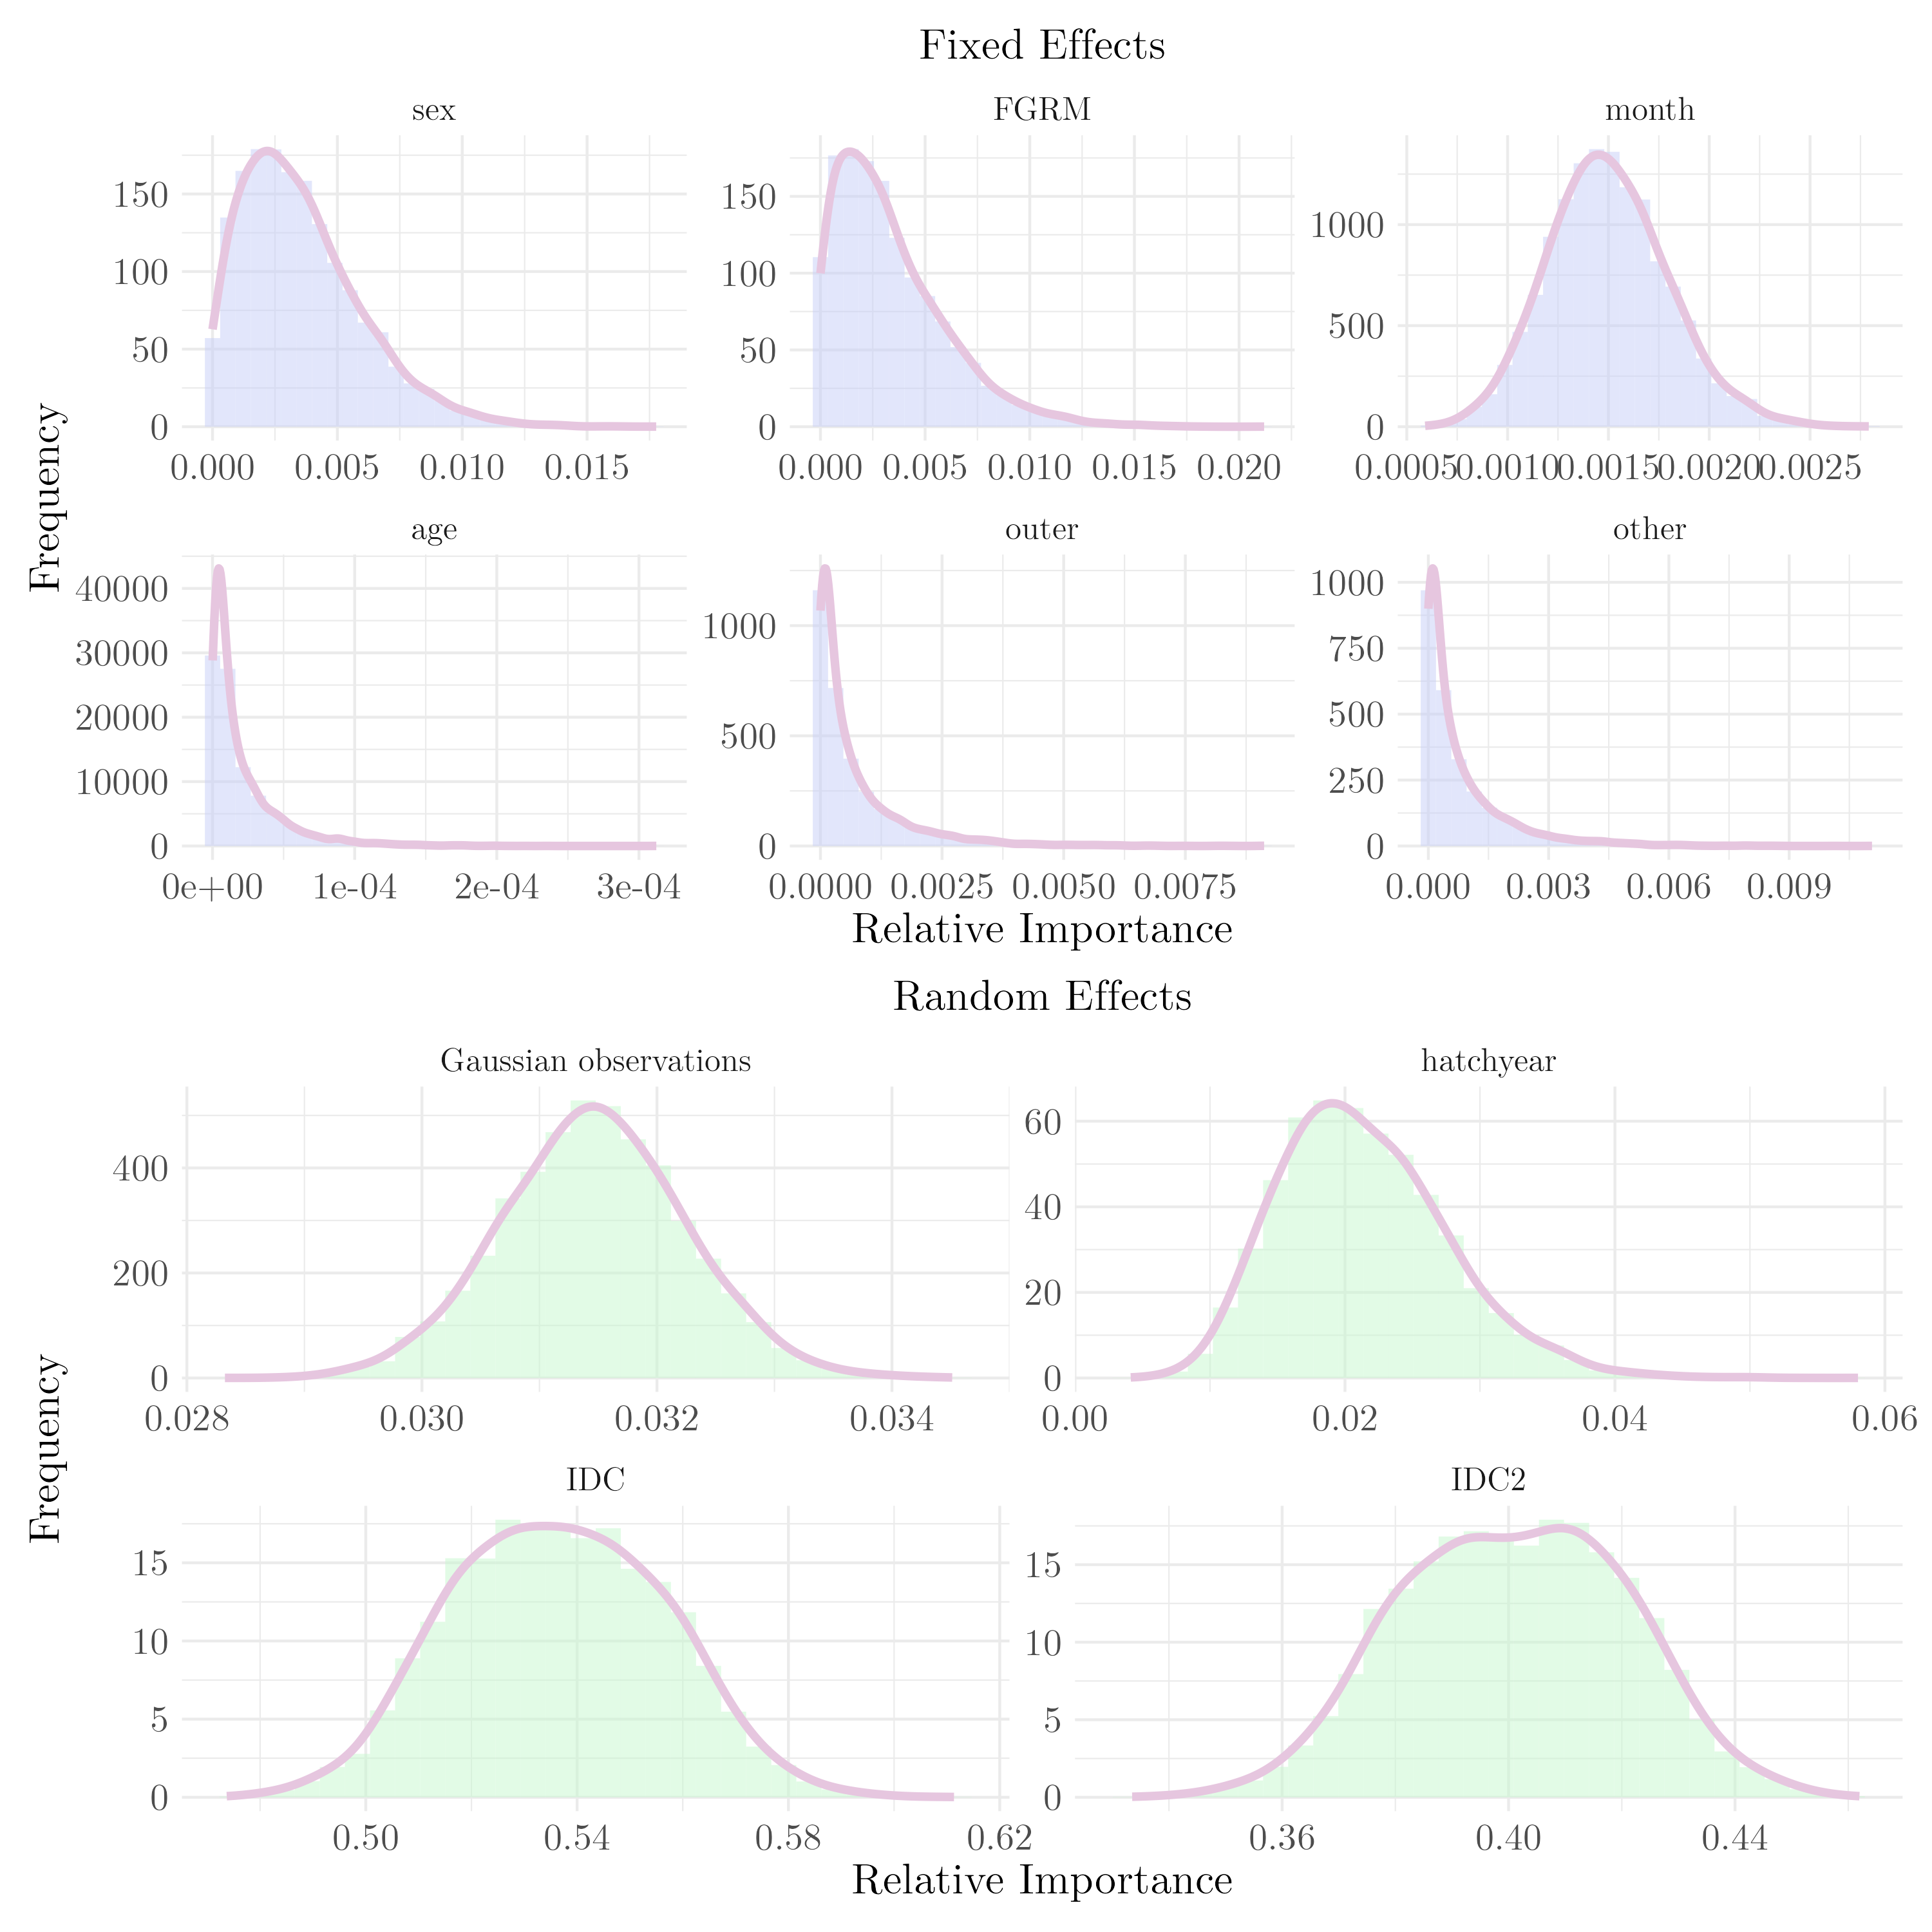
\includegraphics[width=\linewidth]{Figures/House sparrow study/Tarsus_ccd.png}
  \caption[Estimated posterior importance of all covariates in the tarsus length model from the BVI method]{Histogram of the sampled posterior importance values for covariates used in the tarsus length model of the house sparrows, estimated by the BVI method. The heritability estimates correspond to the random effect \textit{IDC2}, and the estimates from the BVI method and \citet{Silva2017} of heritability are found in \Cref{table:summary_heritability}. No estimate from \citet{Muff2019Genetic} was available.}
  \label{fig:heritability_tarsus_combined}
\end{figure}
% \begin{figure}[H]
%   \centering
%   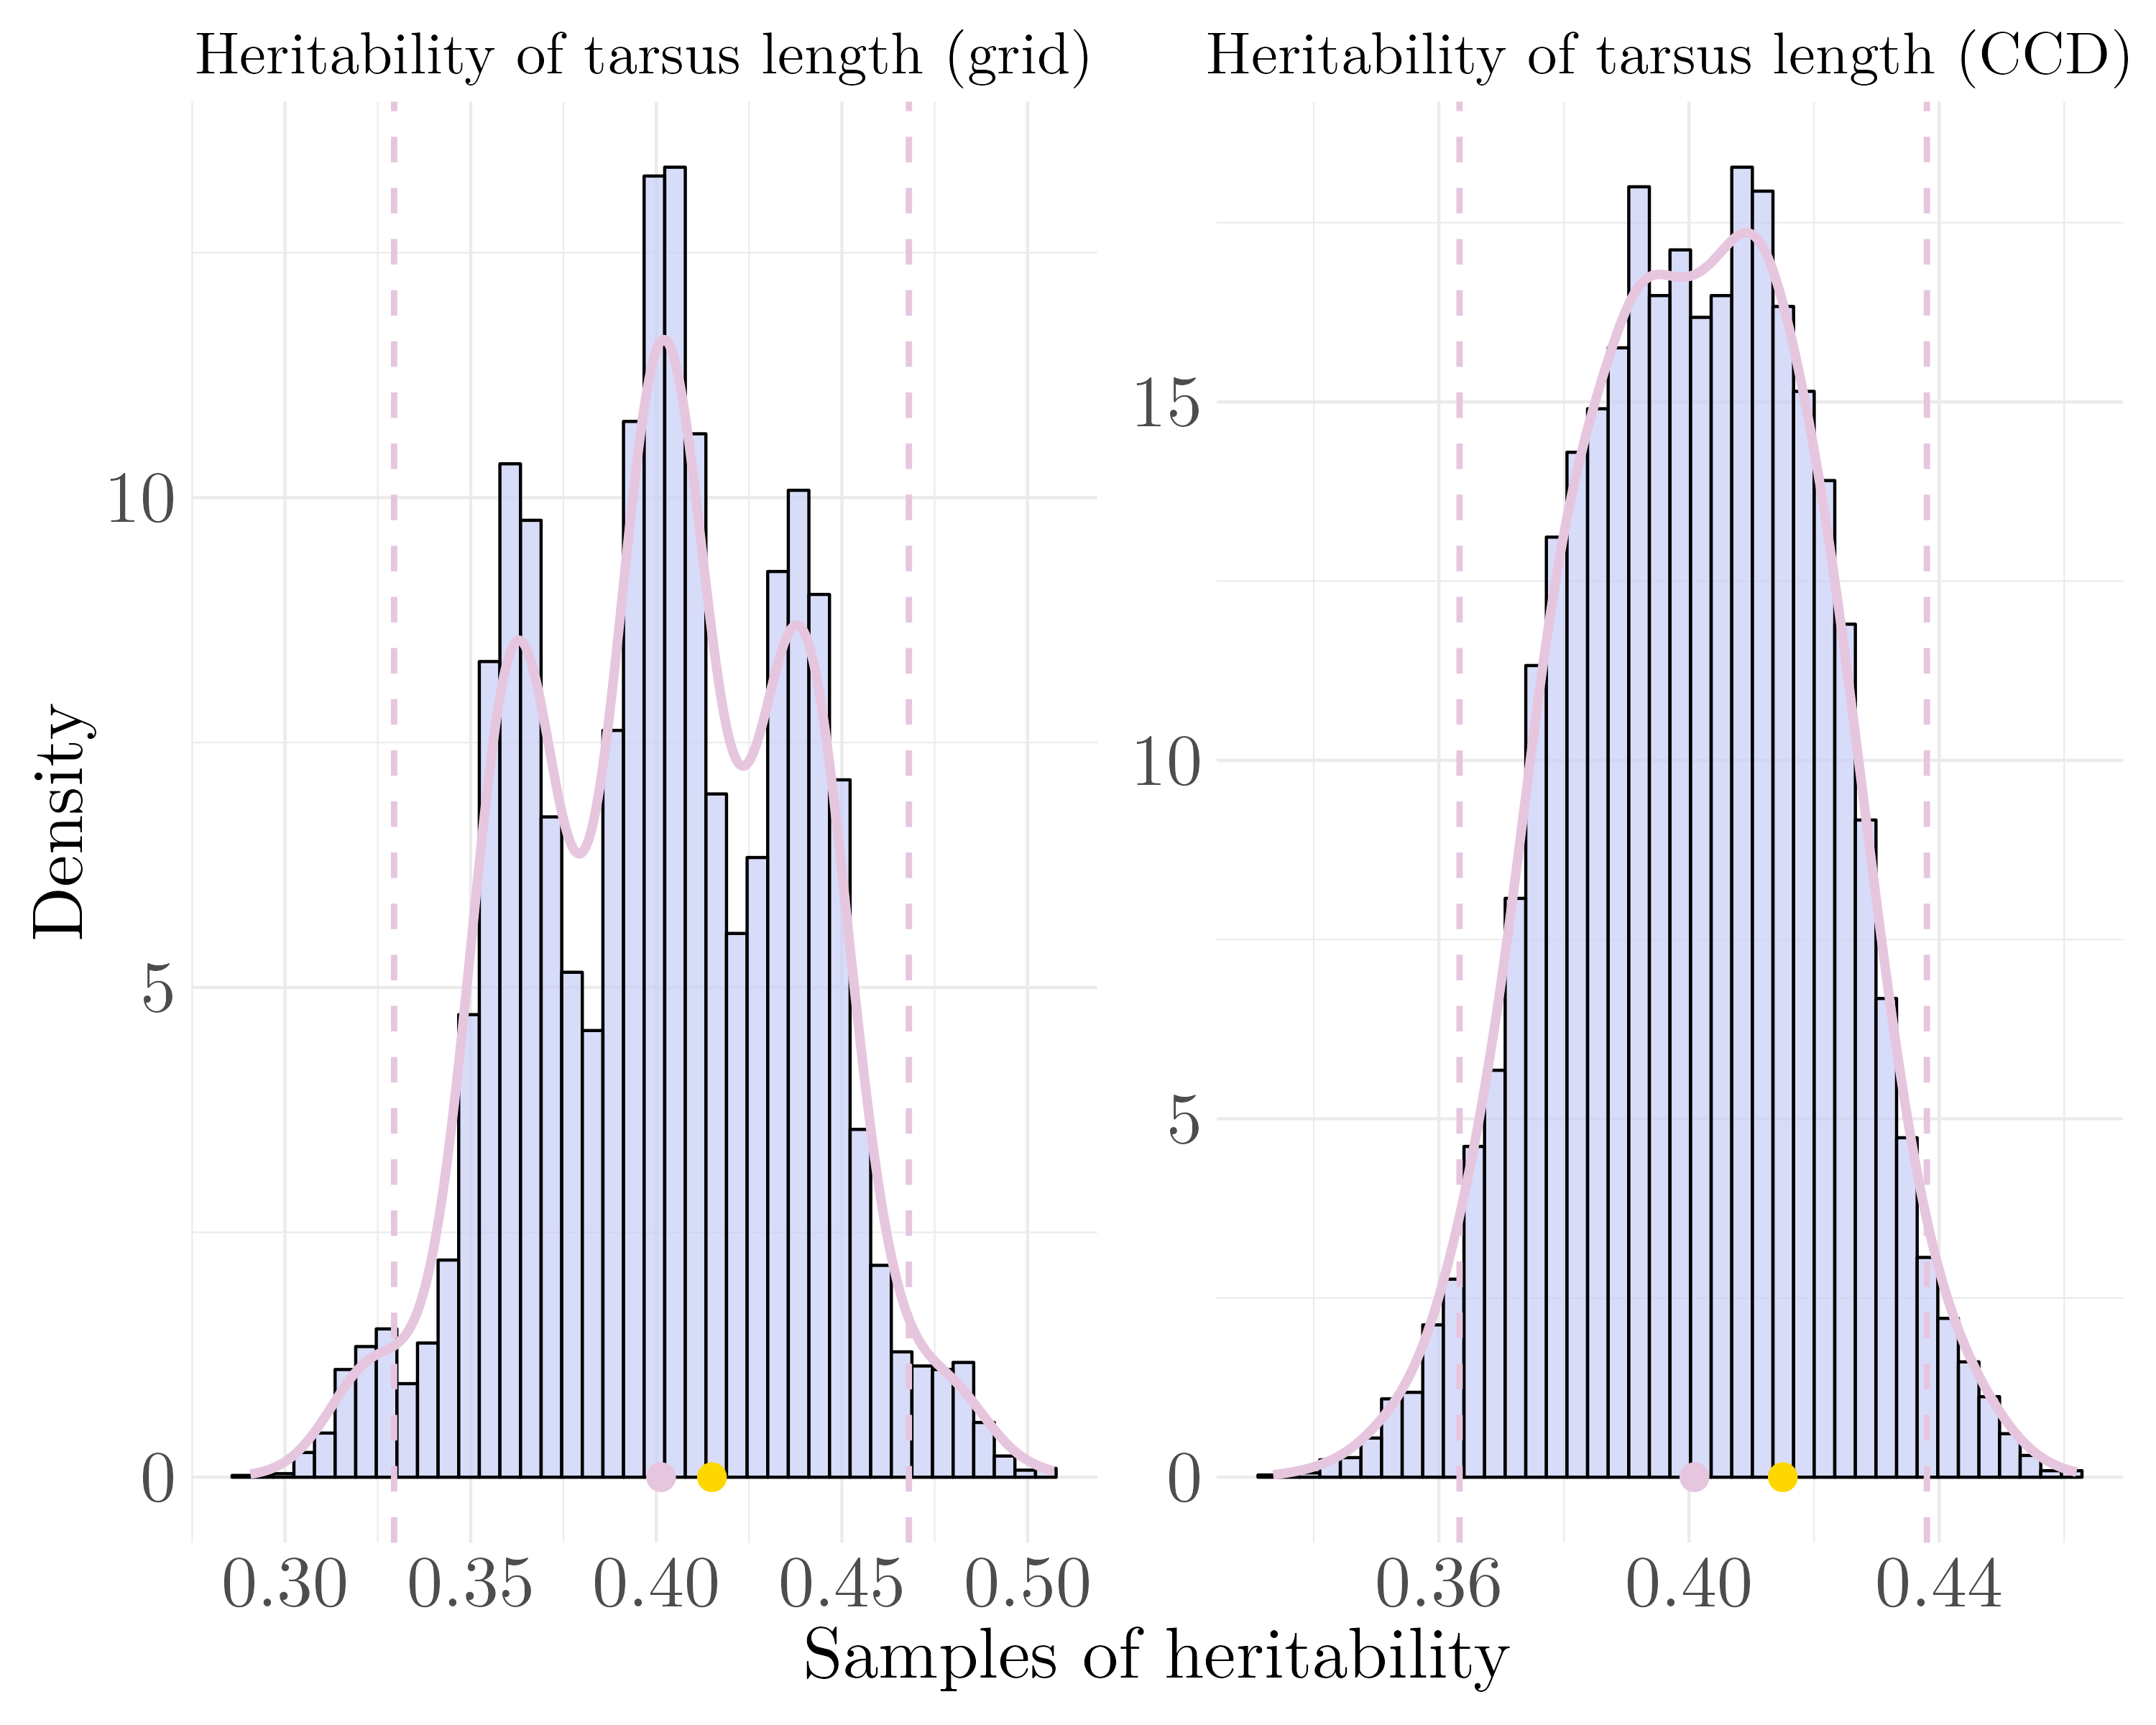
\includegraphics[width=\linewidth]{Figures/House sparrow study/Heritability_tarsus_combined.png}
%   \caption[Estimated heritability of tarsus length]{Histogram showing estimated heritability values for tarsus length of the house sparrows from the BVI method for the grid integration strategy (left) and the CCD integration strategy (right). The two dots at the bottom represent the mean of the samples (pink) and the estimate from \citep{Silva2017} (gold). The dashed lines represent the lower and upper value for the $95\%$ percentile.}
%   \label{fig:heritability_tarsus_combined}
% \end{figure}
\noindent We see it as natural that some different patterns that are hard to fully interpret occur, as the dataset is from real life and relatively small. Further, the measurements are taken on birds that are quite small, so one should expect measurement error to some degree.

\section{Non-Gaussian simulation study}
In this section, we display the results of our simulation study of a binomial and a Poisson regression. We note that it has been difficult to find suitable methods to compare the non-Gaussian models with, as we are not aware of any method that calculates relative variable importance for all covariates in the same manner. In parallel to fitting our model as described in \Cref{sec:simulation_study}, we fit a model using the \texttt{rptR} package with $100$ bootstrap samples. This allows us to directly compare the importance of the random effect and the marginal and conditional $R^2$ values. However, it does not compute the importance of each fixed effect.  
\subsection{Binomial simulation}
The first model to be analysed is the binomial regression on binary response, modelled with the logit-link function. As mentioned, we fit $N_{sim}=500$ models for each correlation level using the Bayesian Variable Importance method. Then, the BVI method extracts the posterior mode, and calculates the derived measures as described in \Cref{ch:method} to estimate the mode of relative importance for all covariates in each model. A summary of the $500$ estimated modes are shown in the supplementary material (\Cref{ap:supplementary}, specifically \Cref{table:summary_logit}), which contains the mean and values for the lower and upper $95\%$ quantile.
\subsubsection{Fixed effects}
The sampled distribution for the posterior modes of relative importance allocated to the three fixed effects $X_1, X_2$ and $X_3$ are shown for each correlation level (\Cref{fig:fixed_combined_logit}). We see that the distributions generally form a normal shape around the mean, with somewhat varying spread. As correlation levels go from negative to positive, meaning that the variance contribution from the fixed effects increase, the importances of the fixed effects also increase. This is expected, as the marginal $R^2$ increases and is spread across the correlated fixed effects. The difference is quite substantial, with the average relative importance allocated to $X_1$ for $\rho=-0.4$ being $0.020$ compared to $0.173$ for $\rho=0.4$. The same pattern is seen for $X_2$ and $X_3$, with the average relative importance increasing from $0.077$ to $0.239$ for $X_2$ and from $0.166$ to $0.299$ for $X_3$ when going from $\rho=-0.4$ to $\rho=0.4$. For $\rho=0$ (middle plot of \Cref{fig:fixed_combined_logit}), it is clear that the average estimate for relative importance of all fixed effects is very similar to the expected importance (\Cref{table:3}) shown as a dashed green line. 
\\
\\
We notice that the covariates $X_1$ and $X_2$ are allocated a significantly larger share when correlation goes from $\rho=0$ to $\rho=0.4$, whereas $X_3$ is almost unchanged for the same correlation levels. This was also experienced in the simulation study on LMMs in \Cref{sec:simulation_study_gauss} from \citet{Arnstad:Relative_variable_importance_in_Bayesian_linear_mixed_models:2024}. It is explained by the fact that off-diagonal elements of $\boldsymbol{\Lambda}$ increase positively when the fixed effects are positively correlated, while the diagonal elements decrease. In the uncorrelated case, $\boldsymbol{\Lambda}$ should be equal to the identity matrix. The columns of $\boldsymbol{\Lambda}$ therefore act as weights and due to this, when $\rho=0.4$, $X_1$ will receive an importance estimate where $\beta_2^2$ and $\beta_3^2$ will have positive weights contrary to $\rho=0$ where the only weight is put on $\beta_1^2$. Since $\beta_1^2$ is smaller than $\beta_2^2$ and $\beta_3^2$, the higher positive correlation level yields a higher importance estimate for $X_1$. The same pattern is seen for $X_2$, where $\beta_1^2$ is smaller and $\beta_3^2$ is larger than $\beta_2^2$. This means the importance of $X_2$ is estimated to be higher for $\rho=0.4$ than for $\rho=0$, but the increase is smaller than the increase for $X_1$ \citep{Arnstad:Relative_variable_importance_in_Bayesian_linear_mixed_models:2024}. In contrast, the importance of $X_3$ is then estimated with more weight on $\beta_1^2$ and $\beta_2^2$, which are both smaller than $\beta_3^2$, and thus the importance is not notably increased. If one had introduced a larger positive correlation level than $\rho=0.4$, we would therefore expect the importance of $X_3$ to even decrease, as was seen in \citet{Arnstad:Relative_variable_importance_in_Bayesian_linear_mixed_models:2024}. It is hard to say, based on these results, whether the inverse pattern can be seen for negative correlation levels, but it could be noted that the decrease in importance is less for $X_3$ compared to $X_1$ and $X_2$ when $\rho$ changes from $0$ to $-0.1$.
\\
\\
Generally, it seems that the method is able to capture the expected effects of varying correlation levels, and is in close agreement with the expected theoretical values when the fixed effects are uncorrelated. 
\begin{figure}[H]
  \centering
  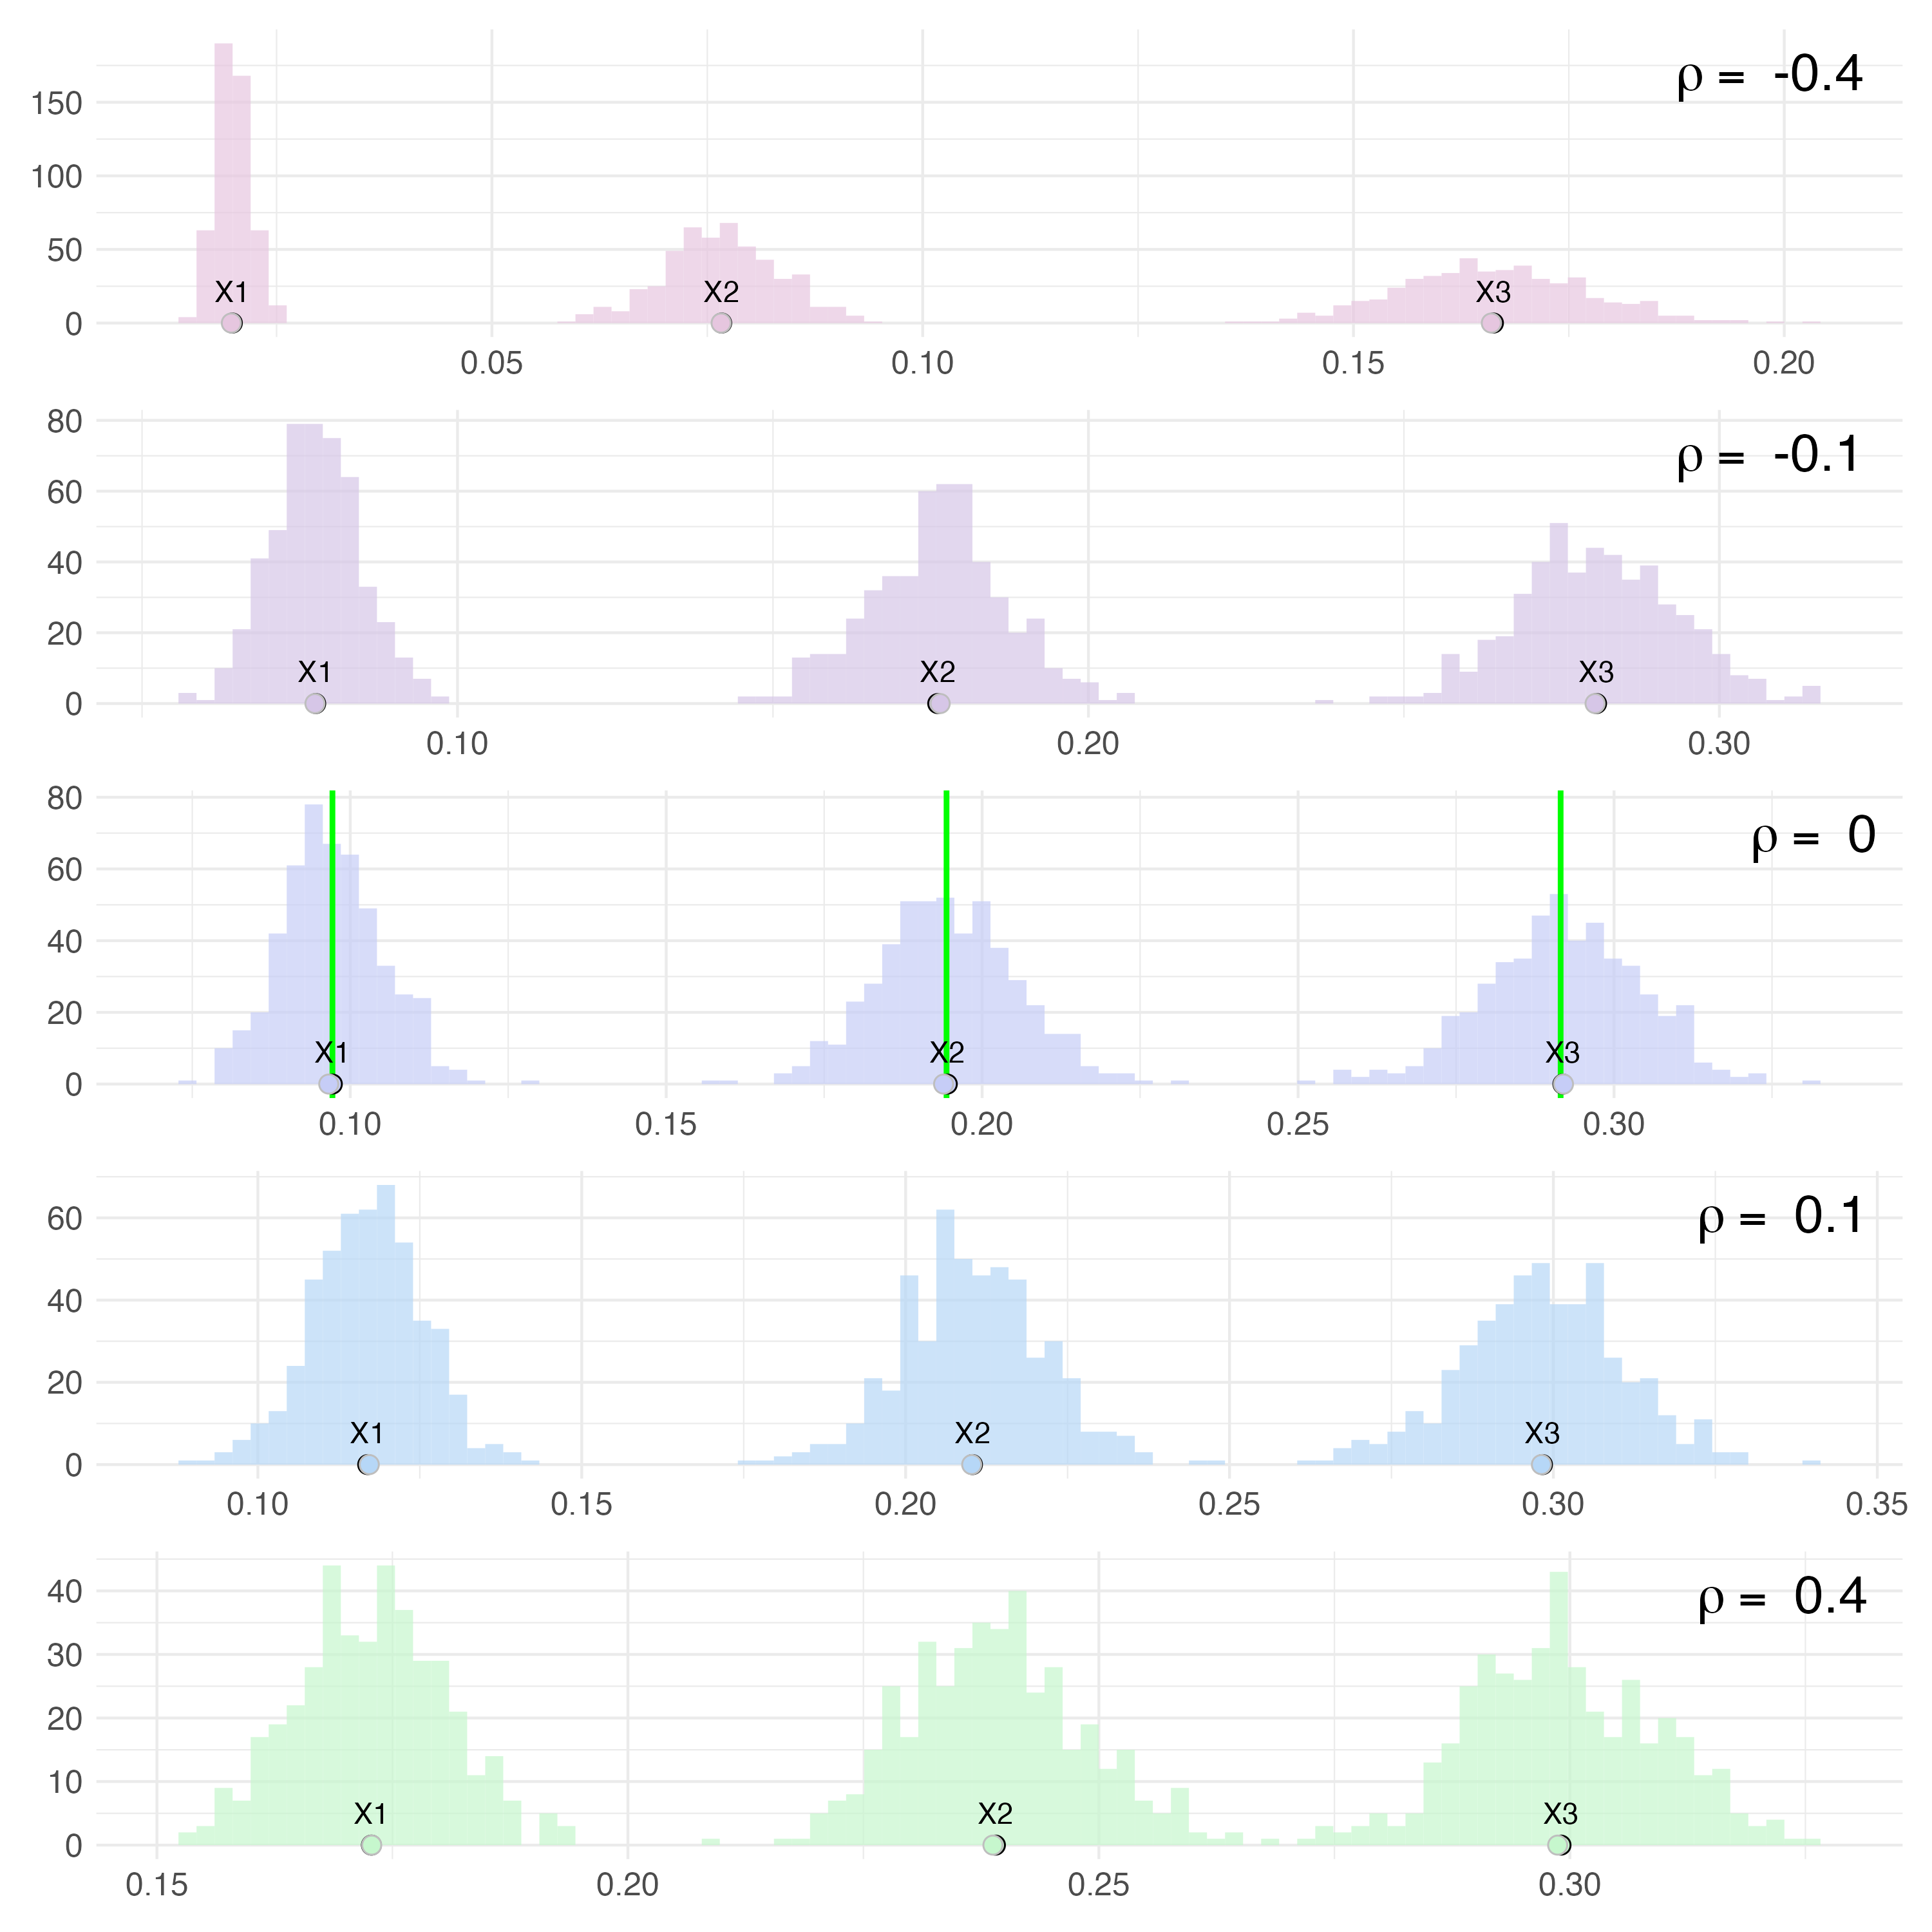
\includegraphics[width=1.1\linewidth]{Figures/Simulation study/Fixed_combined_logit.png}
  \caption[Relative importance of the fixed effects in binomial GLMM]{Histogram with the distribution of posterior modes of relative importance for the fixed effects present in the binomial regression for the different correlation levels $\rho$. The modes of relative importance are calculated by the Bayesian Variable Importance method from the $N_{\text{sim}}=500$ simulations in the simulation study. The vertical green line for $\rho=0$ displays the expected relative importance in the case of uncorrelated data. The mean of the mode values for all simulations is denoted at the bottom of each histogram as a circle.}
  \label{fig:fixed_combined_logit}
\end{figure}
  %\label{fig:fixed_effects_logit}
%\end{figure}
\subsubsection{Random effect}
The sampled posterior modes of importances for the random effect in the logit model (\Cref{fig:relimp_random_logit}) all seem to be roughly normally distributed around the mean. The spread of the random effects seem to be larger than the spread seen in the fixed effects for negative correlations, and more similar for independent and positively correlated covariates. One can see that when the correlation in fixed effects go from negative to positive, the estimated importance of the random effect shrinks. Specifically, when $\rho=-0.4$ the average estimate of relative importance for the random effect is $0.171$ compared to only $0.067$ when $\rho=0.4$. This naturally occurs as the variance contribution from the random effect should be held constant for the correlation levels, and the variance contribution from the fixed effects rise as the correlation increases. Therefore, the proportion of variance explained, which is our definition of relative variable importance, will decrease for the random effect. For $\rho=0$ we see that the average relative importance estimate lies very near the expected value of $0.097$ (\Cref{table:3}). The orange dot at the bottom of the histograms in \Cref{fig:relimp_random_logit} displays the estimated relative importance of the fixed effect from the \texttt{rptR} package, and we see that the estimates are quite close to the mean of the BVI method. The largest difference from the BVI and the \texttt{rptR} package is $0.021$ and are found when $\rho=0$. This difference is $22\%$ of the average estimated relative importance from the BVI method, and is therefore not negligible. However, the methods seem to be in agreement for the overall trends and the methods are closer in accordance with each other for the other correlation levels.
\\
\\
\begin{figure}[H]
  \centering
    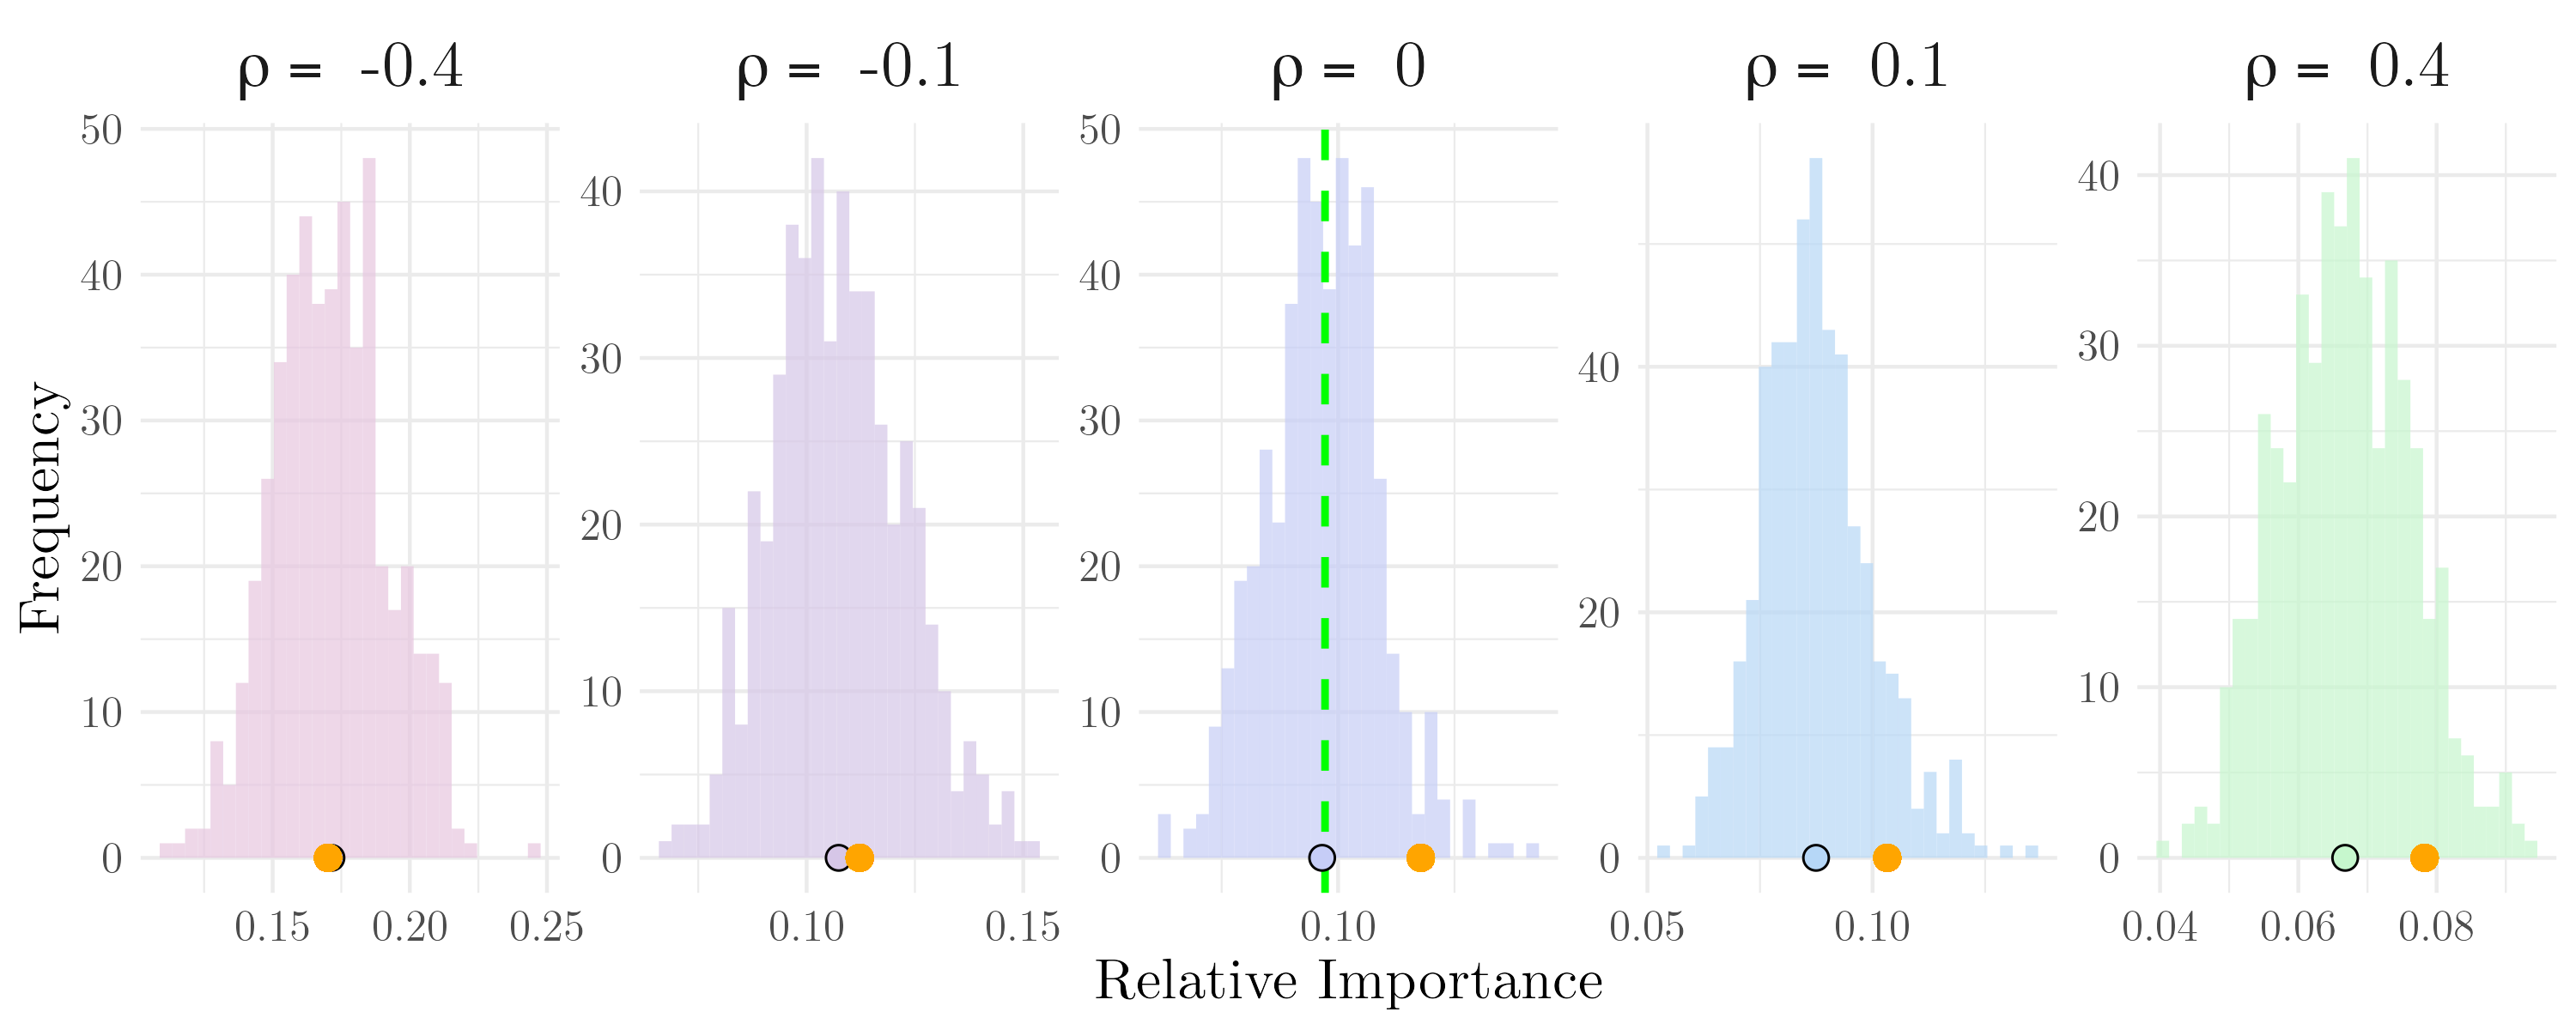
\includegraphics[width=1\linewidth]{Figures/Simulation study/Random_logit.png}
    \caption[Relative importance of the random effect $\boldsymbol{\alpha}$ in binomial GLMM]{Histogram with the posterior modes from the BVI method for each of the $N_{\text{sim}}=500$ simulations, estimating relative importance of the random effect $\boldsymbol{\alpha}$ across the different correlation levels $\rho$. The mean of the mode values from all simulations is displayed at the bottom as a circle and the orange dot at the bottom displays the estimate from the \texttt{rptR} package. The vertical green line for $\rho=0$ is the expected relative importance as in \Cref{table:3}.}
    \label{fig:relimp_random_logit}
\end{figure}
\subsubsection{$R^2$ estimates}
An important measure in this simulation study is the modes for the sampled posterior distribution of marginal and conditional $R^2$ (\Cref{fig:r2_combined_logit}). The expected values for the marginal and conditional $R^2$ are shown in \Cref{table:r2values}, and are displayed as vertical green lines in each plot. It is clear that, regardless of correlation level, the BVI method is able to estimate the marginal and conditional $R^2$ close to what we expect. The distributions of $R^2$ values seem to have the shape of a bell curve and are symmetric around the mean value. The spread is naturally larger than for the individual fixed effects and random effects, as the $R^2$ is constructed from these importances. For both the marginal and conditional $R^2$ estimates, there is only a negligible difference between the results from the BVI method and the expected values. When comparing to the results from the \texttt{rptR} package, there are some larger differences. The marginal $R^2$ deviates the most when $\rho=0$ with a difference of $0.014$, which is $3\%$ of the average estimated value. For the conditional $R^2$ the largest difference is $0.018$ which also makes up $3\%$ of the average estimated value, found for $\rho=0.1$. Generally, the BVI method seems to be in line with our expectation for $R^2$ values, deviating slightly more from the \texttt{rptR} package estimates.
% it seems that the BVI method consistently estimates larger $R^2$ values both marginally and conditionally. The largest difference in means between the BVI and the \texttt{rptR} estimates for the marginal $R^2$ is found when $\rho=0$ and is $0.0448$ which makes up $7\%$ of the average estimated value. For $\rho=-0.4$, the mean difference accounts for $14\%$ of the average estimated marginal $R^2$ value. For the conditional $R^2$ the largest difference is $0.0617$ and found for $\rho=-0.4$, which also makes up $14\%$ of the average estimated value. Generally, the BVI method seems to be in line with our expectation for $R^2$ values, but deviates somewhat from the \texttt{rptR} package estimates.
% \begin{figure}[H]
%   \centering
%   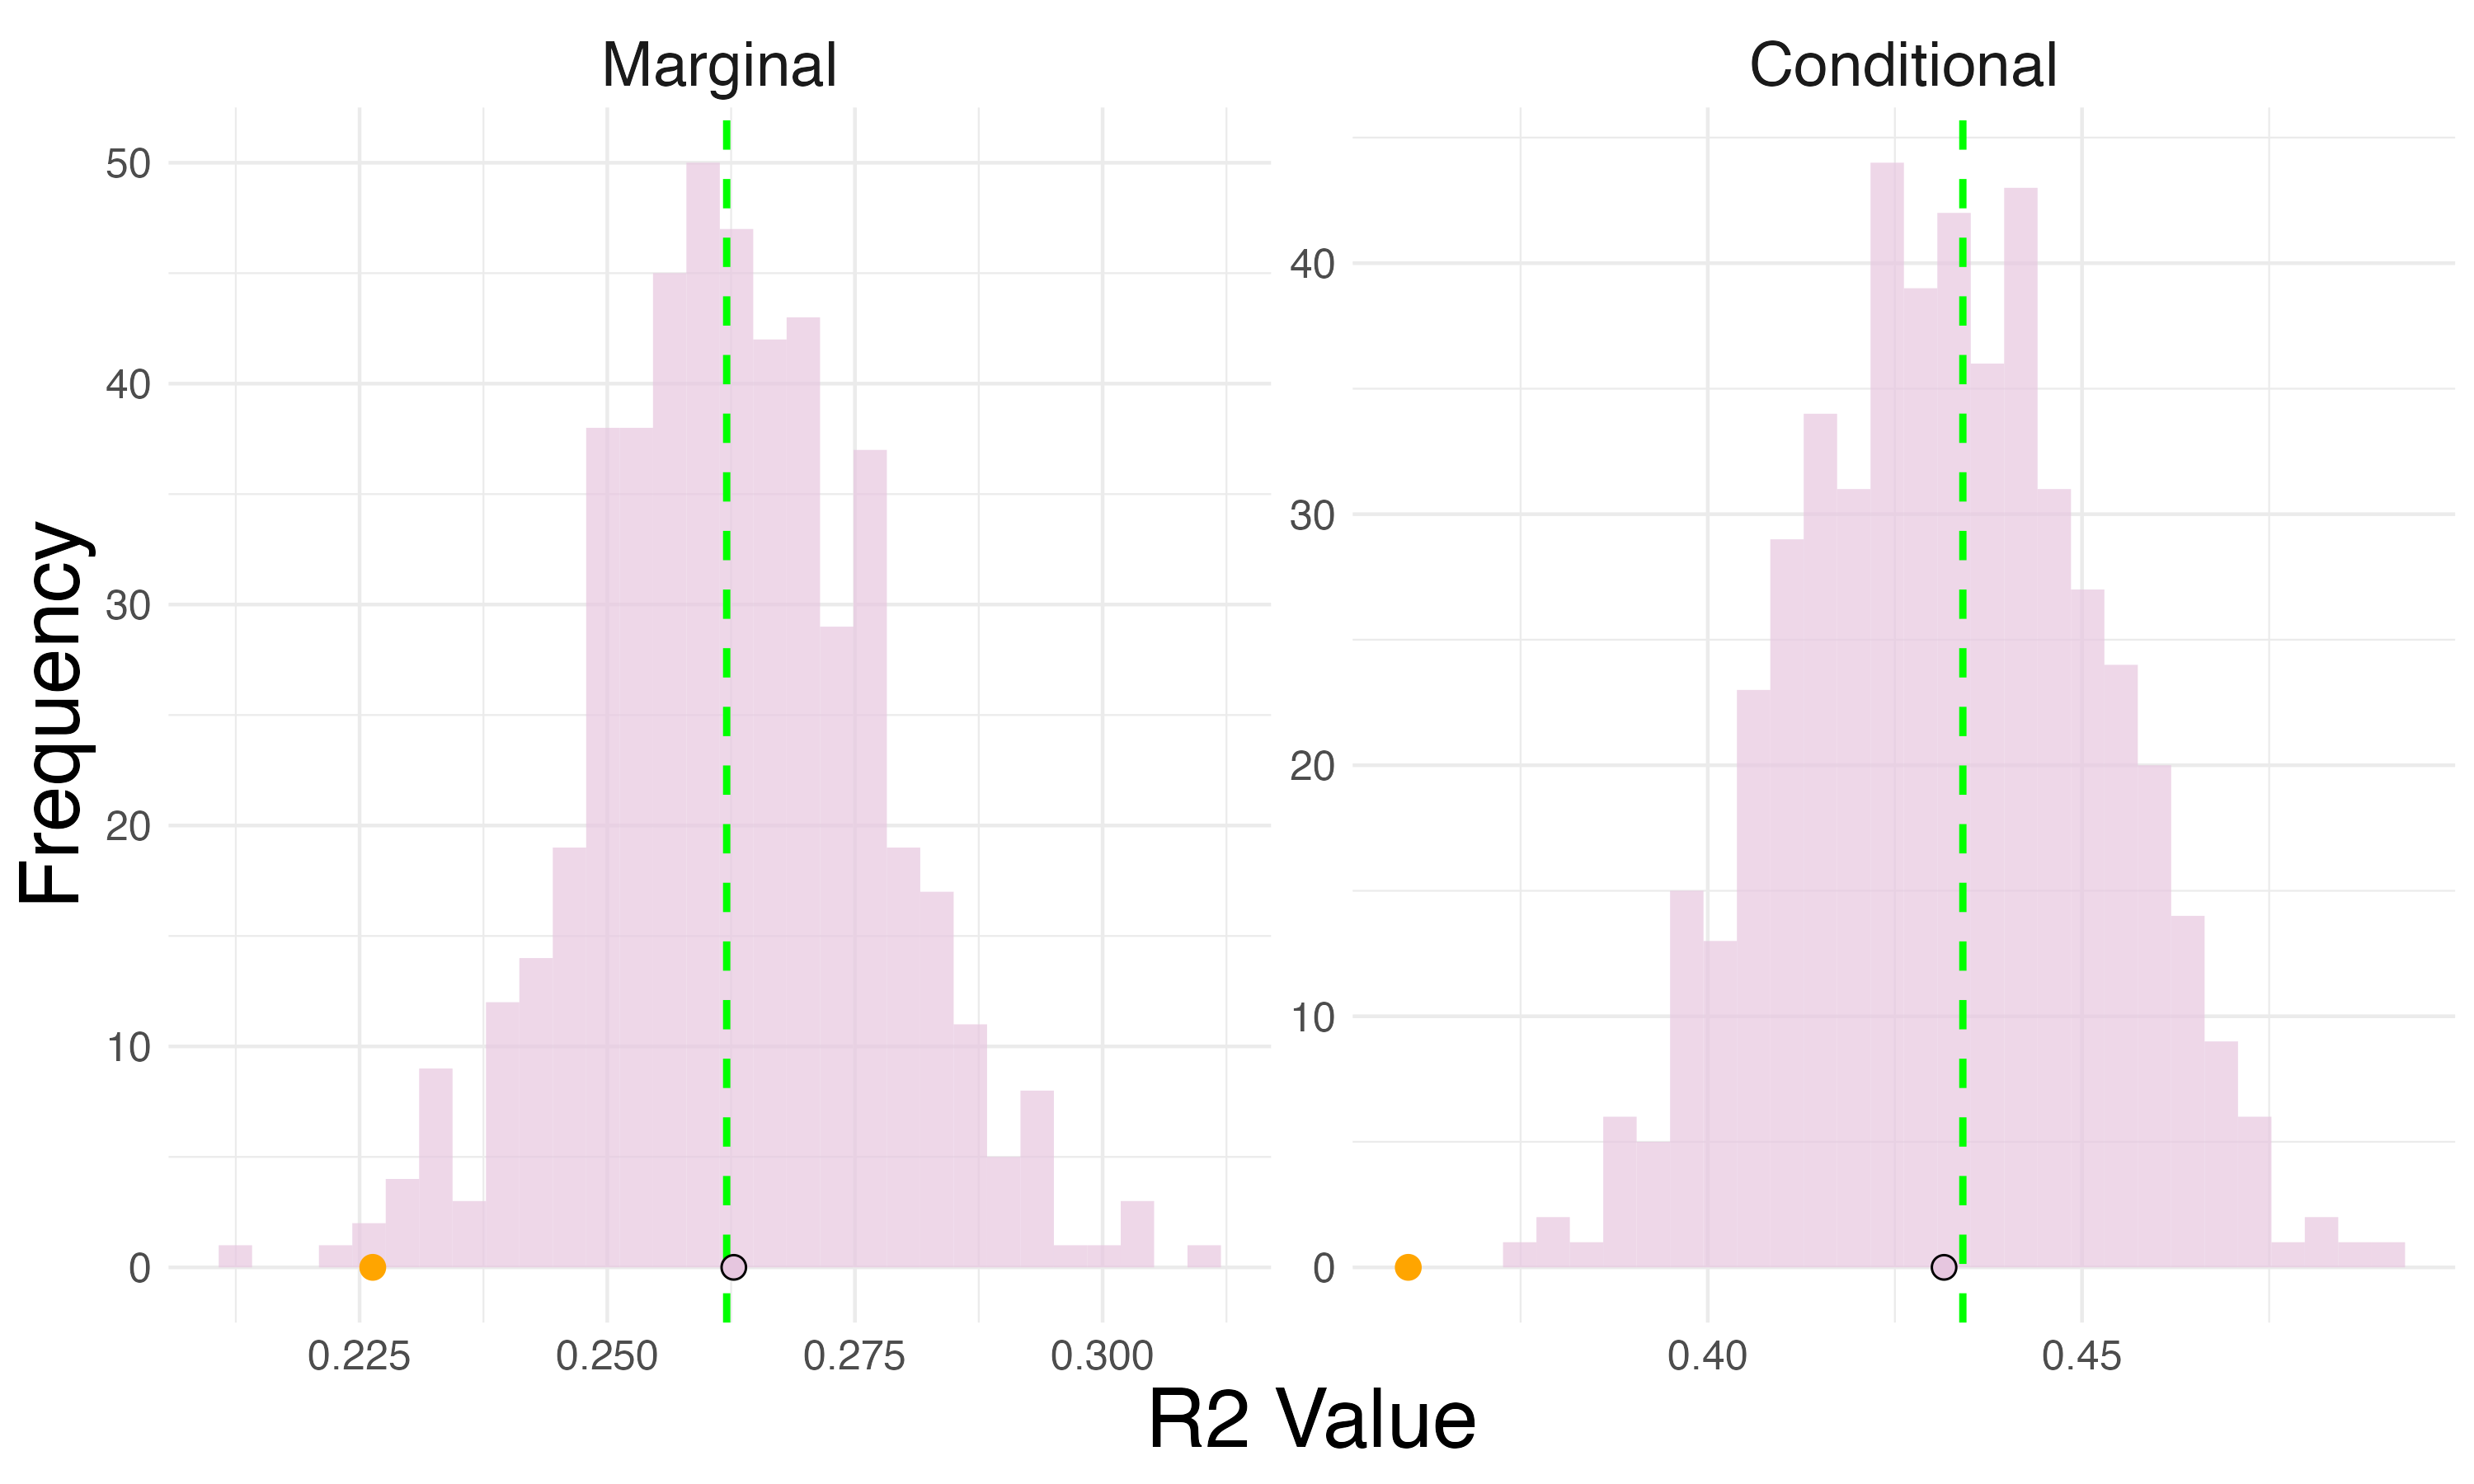
\includegraphics[width=1\linewidth]{Figures/Simulation study/R2_logit_high_neg.png}
%   \caption{Histogram with the estimated marginal $R^2$ (left) and conditional $R^2$ (right) from the BVI method for the binomial regression for the different correlation levels $\rho$ across $N_{\text{sim}}=500$ simulations. The expected values are displayed as vertical green lines, and can be found in \Cref{table:r2values}. The mean value of the $R^2$ values for all simulations is marked with a circle at the bottom. (a) Marginal and conditional $R^2$ estimates for $\rho=-0.4$.}
%   \label{fig:r2_logit_high_neg}
% \end{figure}
% \begin{figure}[H]\ContinuedFloat
%   \centering
%   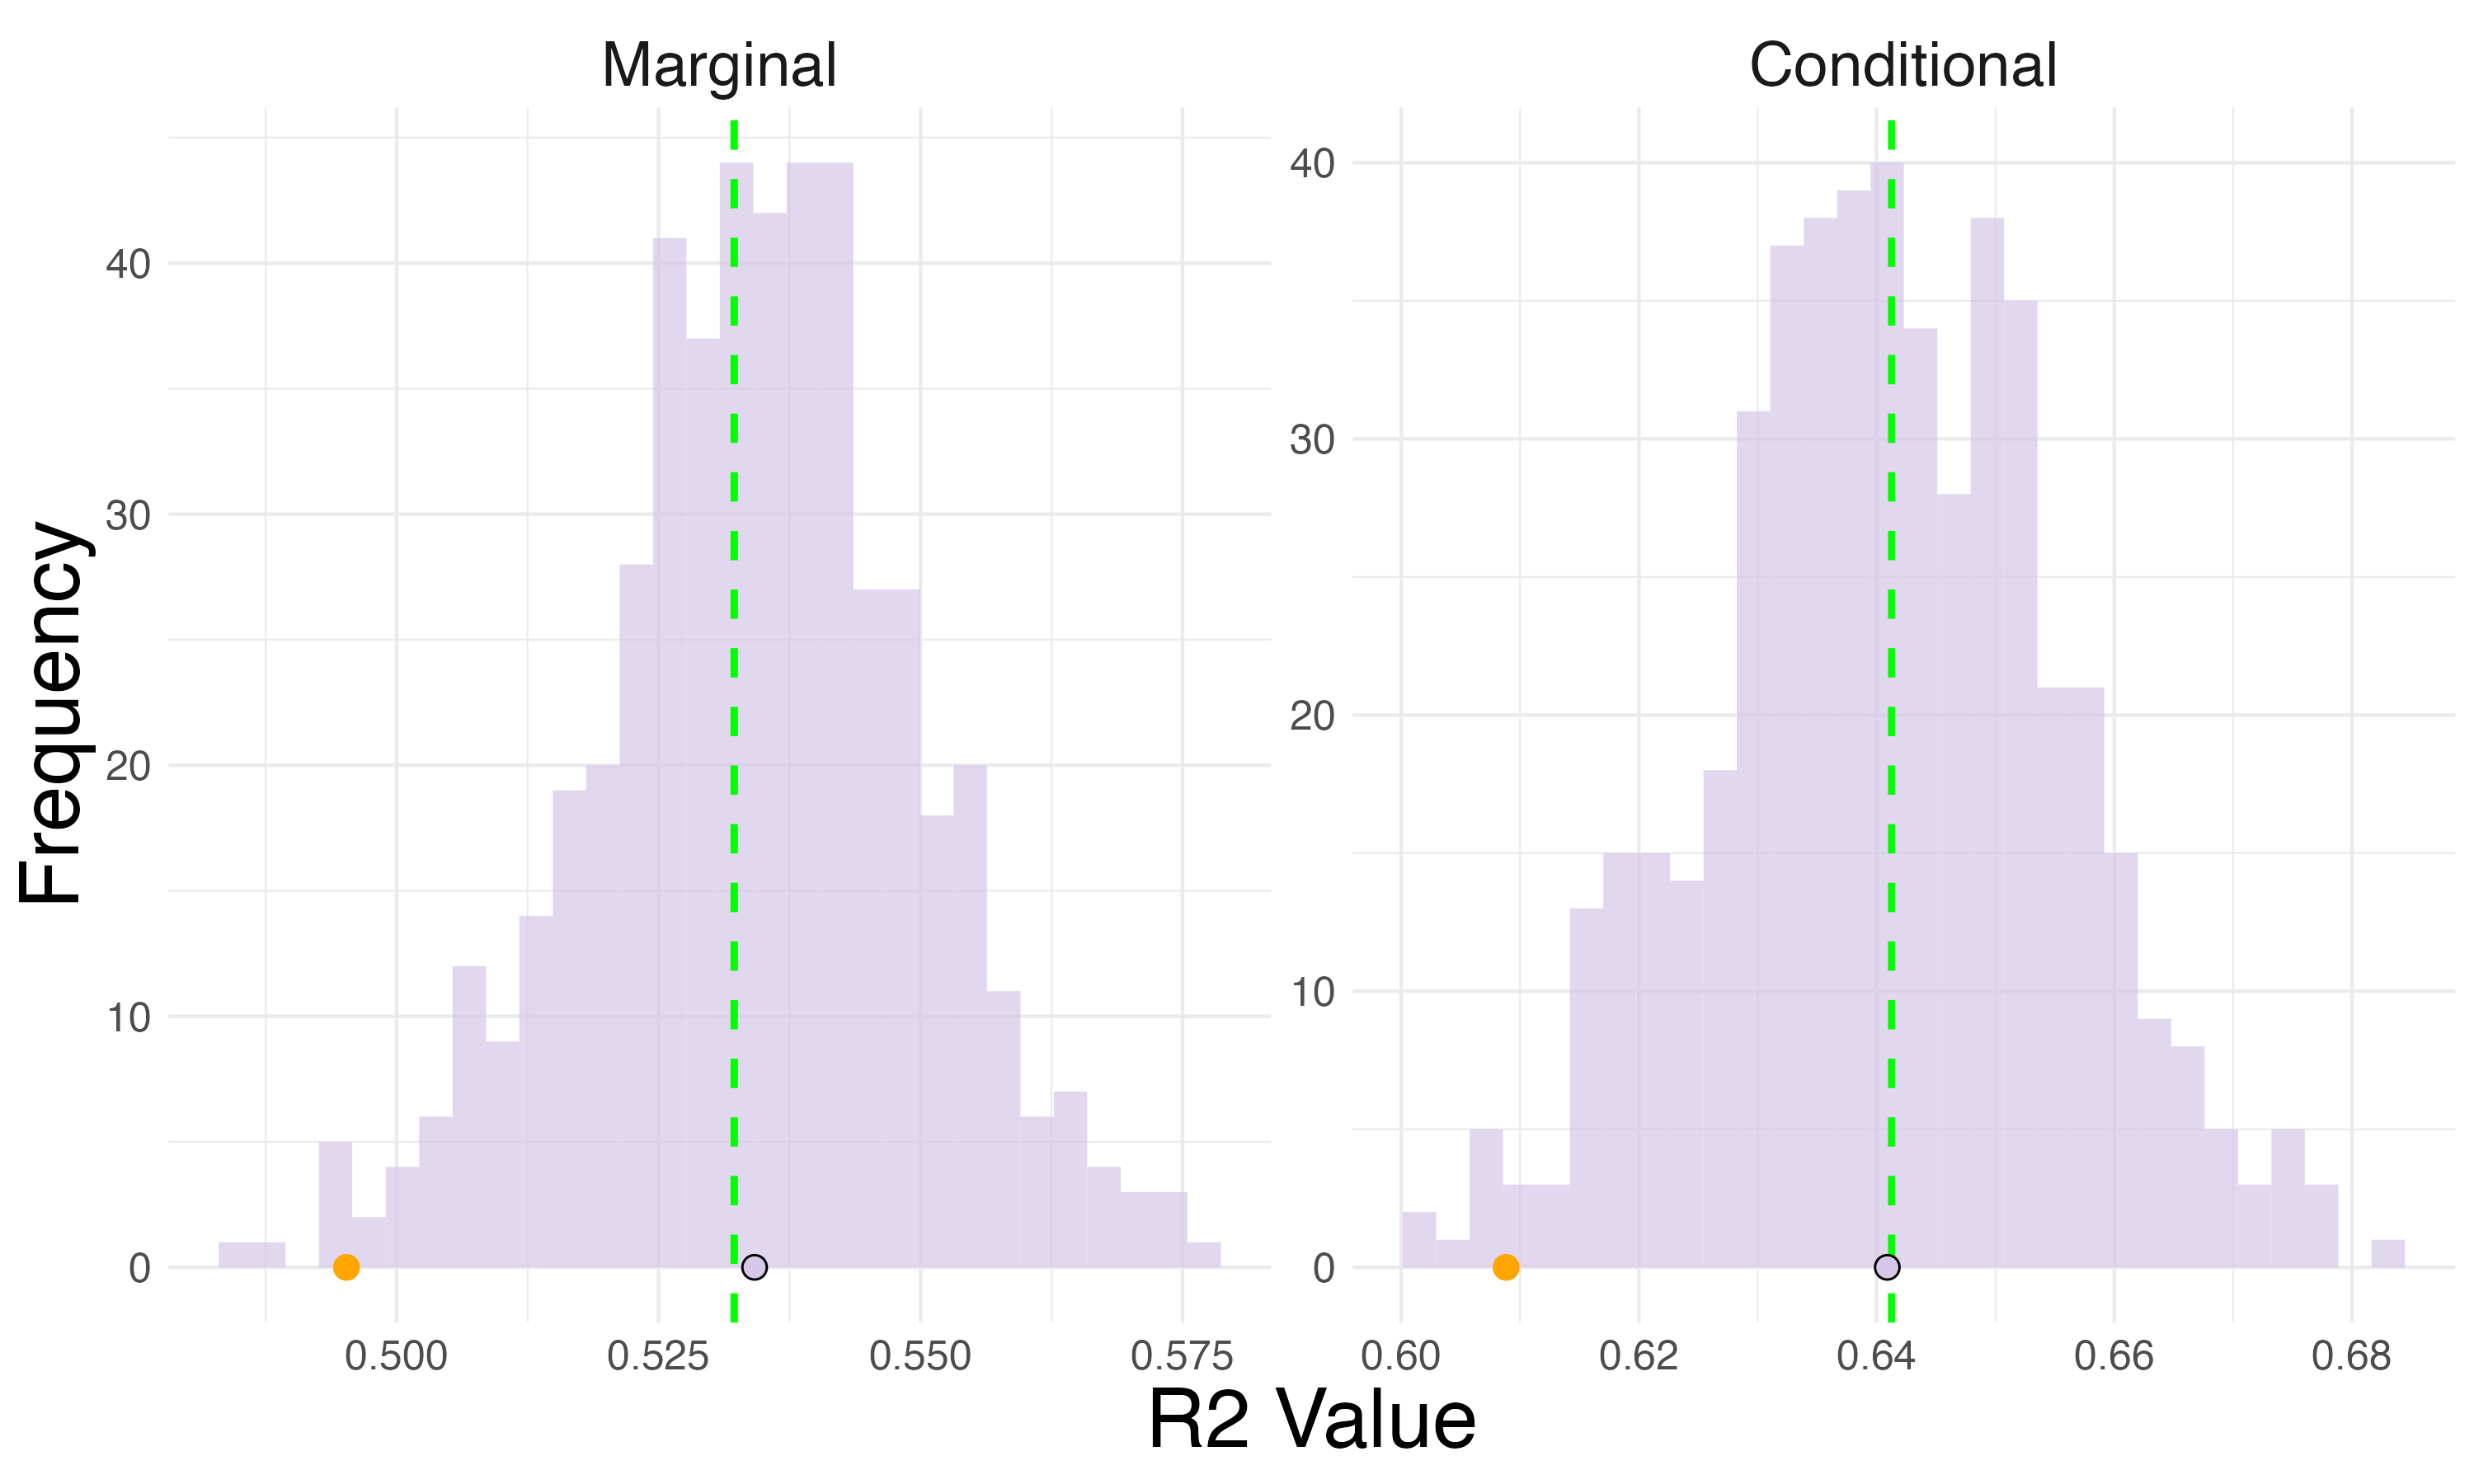
\includegraphics[width=1\linewidth]{Figures/Simulation study/R2_logit_low_neg.png}
%   \caption{(b) Marginal and conditional $R^2$ estimates for $\rho=-0.1$.}
%   \label{fig:r2_logit_low_neg}
% \end{figure}
% \begin{figure}[H]\ContinuedFloat
%   \centering
%   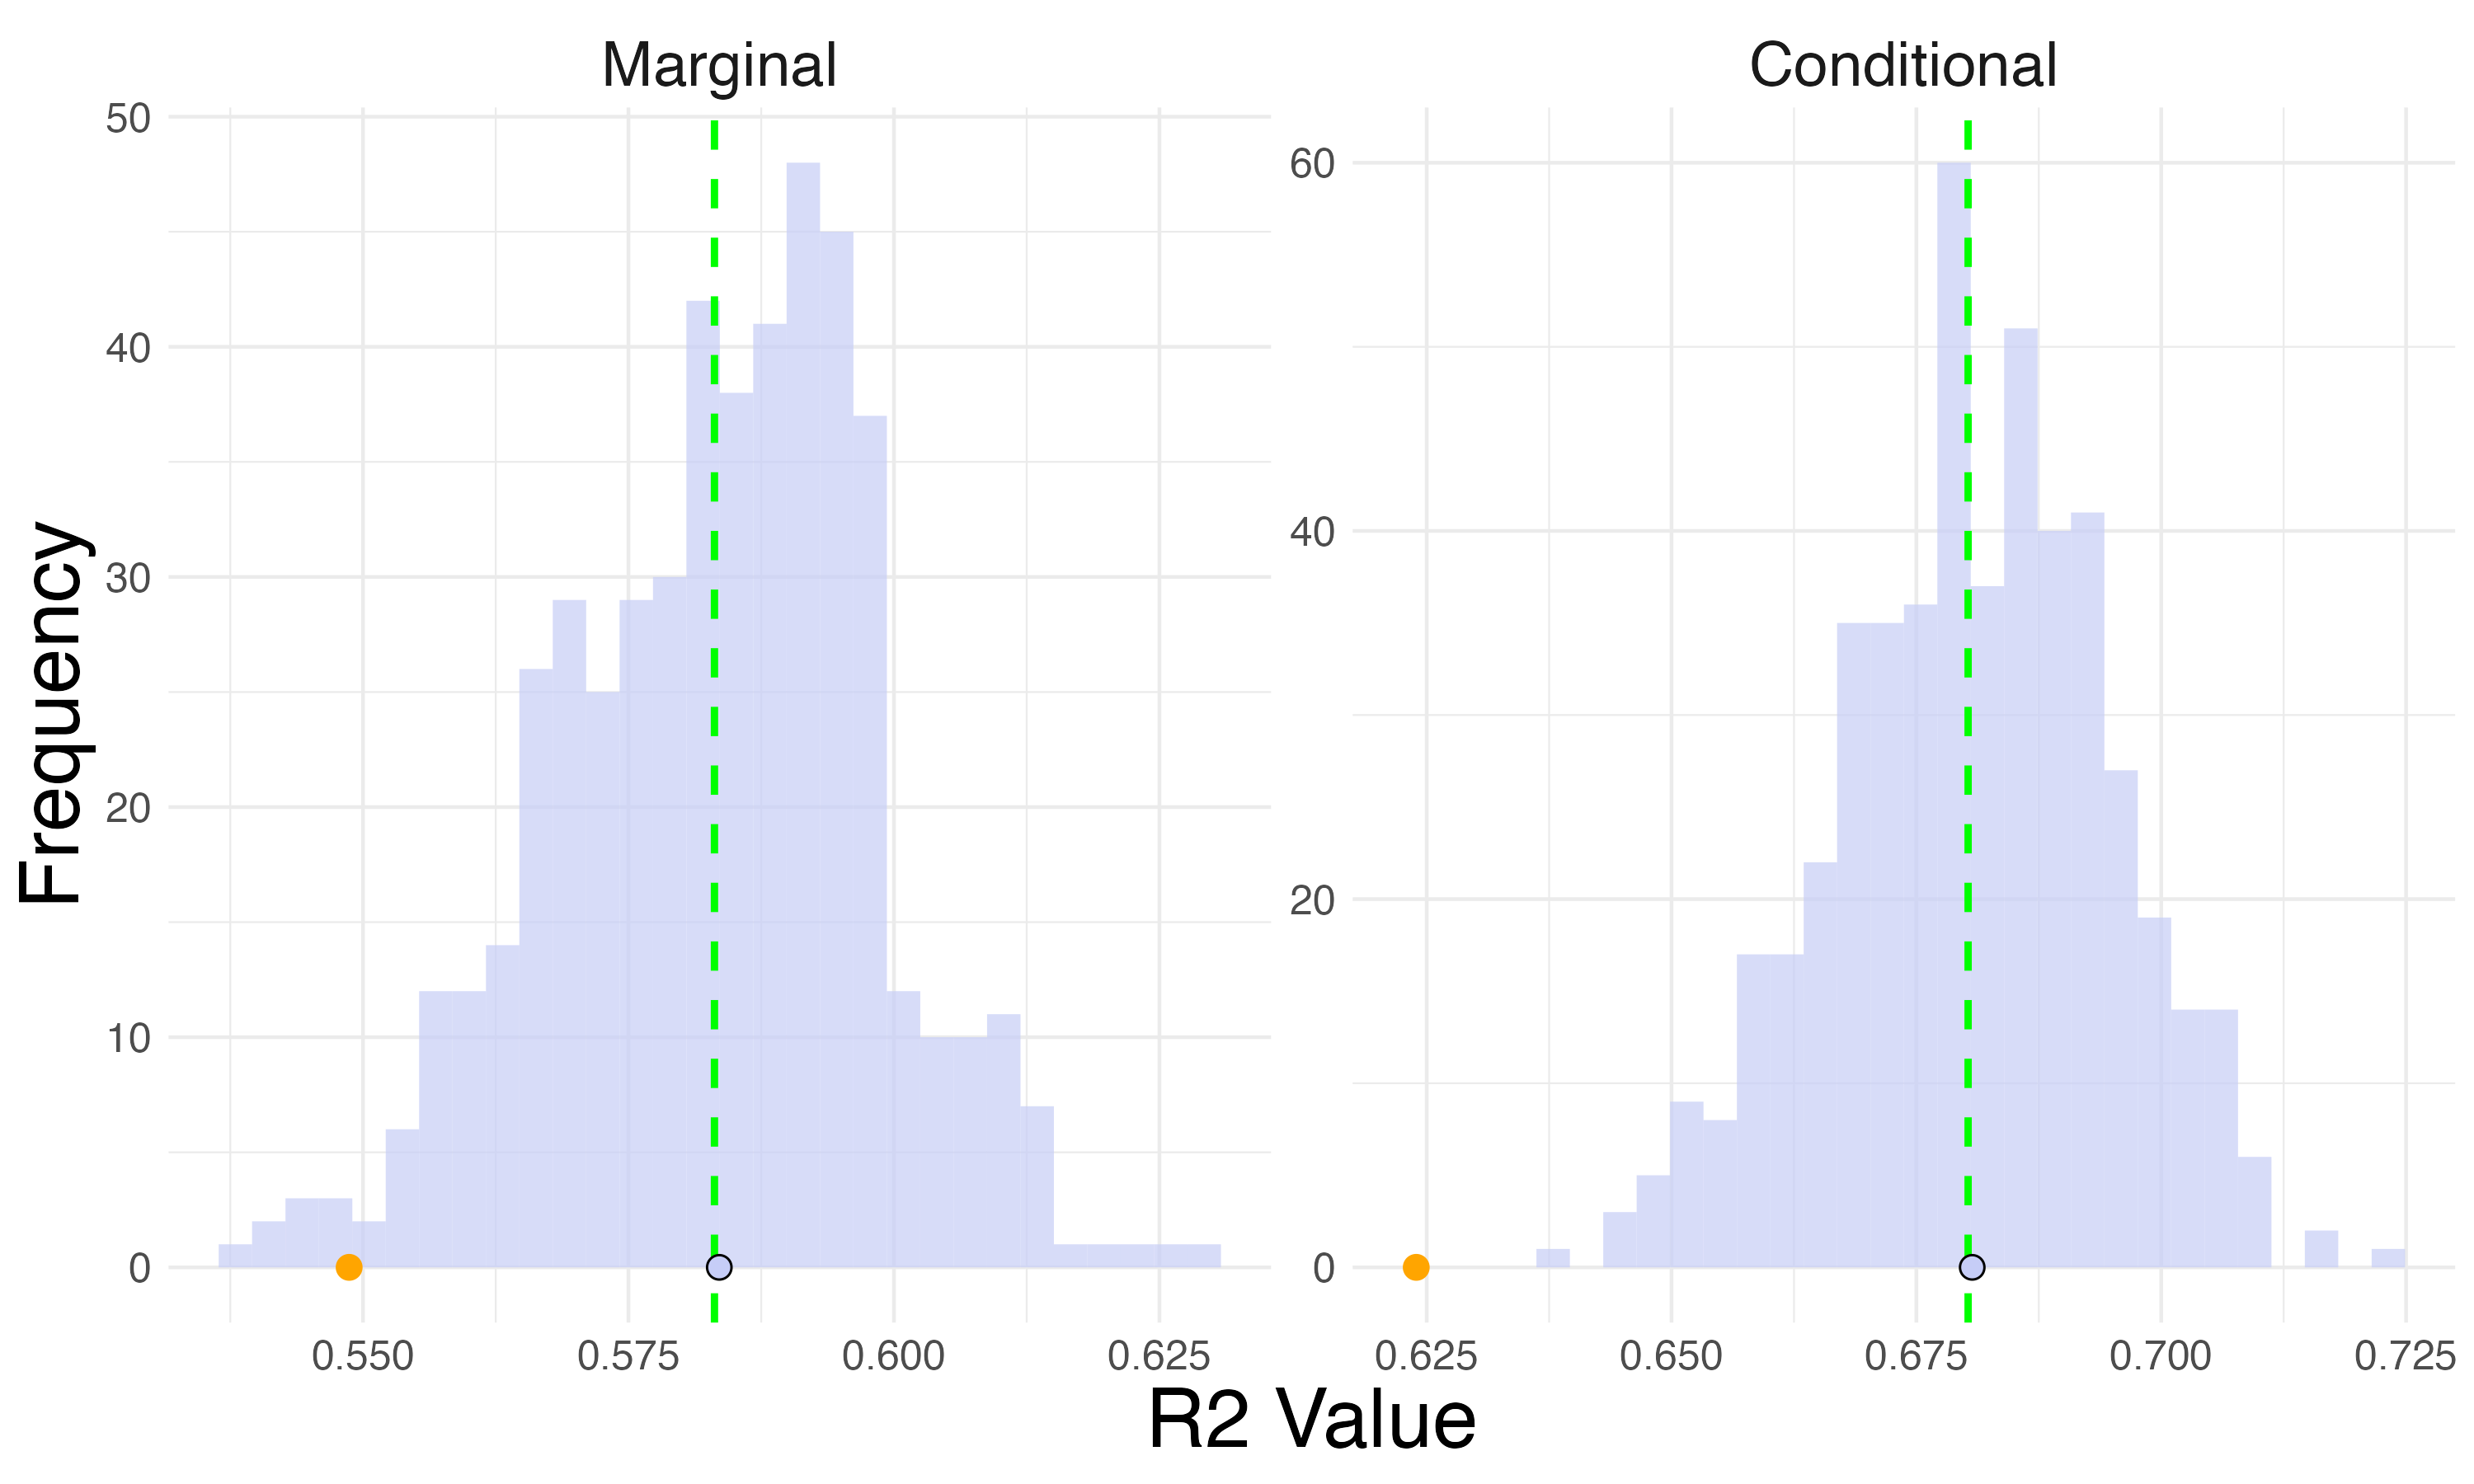
\includegraphics[width=1\linewidth]{Figures/Simulation study/R2_logit_no.png}
%   \caption{(c) Marginal and conditional $R^2$ estimates for $\rho=0$.}
%   \label{fig:r2_logit_no}
% \end{figure}
% \begin{figure}[H]\ContinuedFloat
%   \centering
%   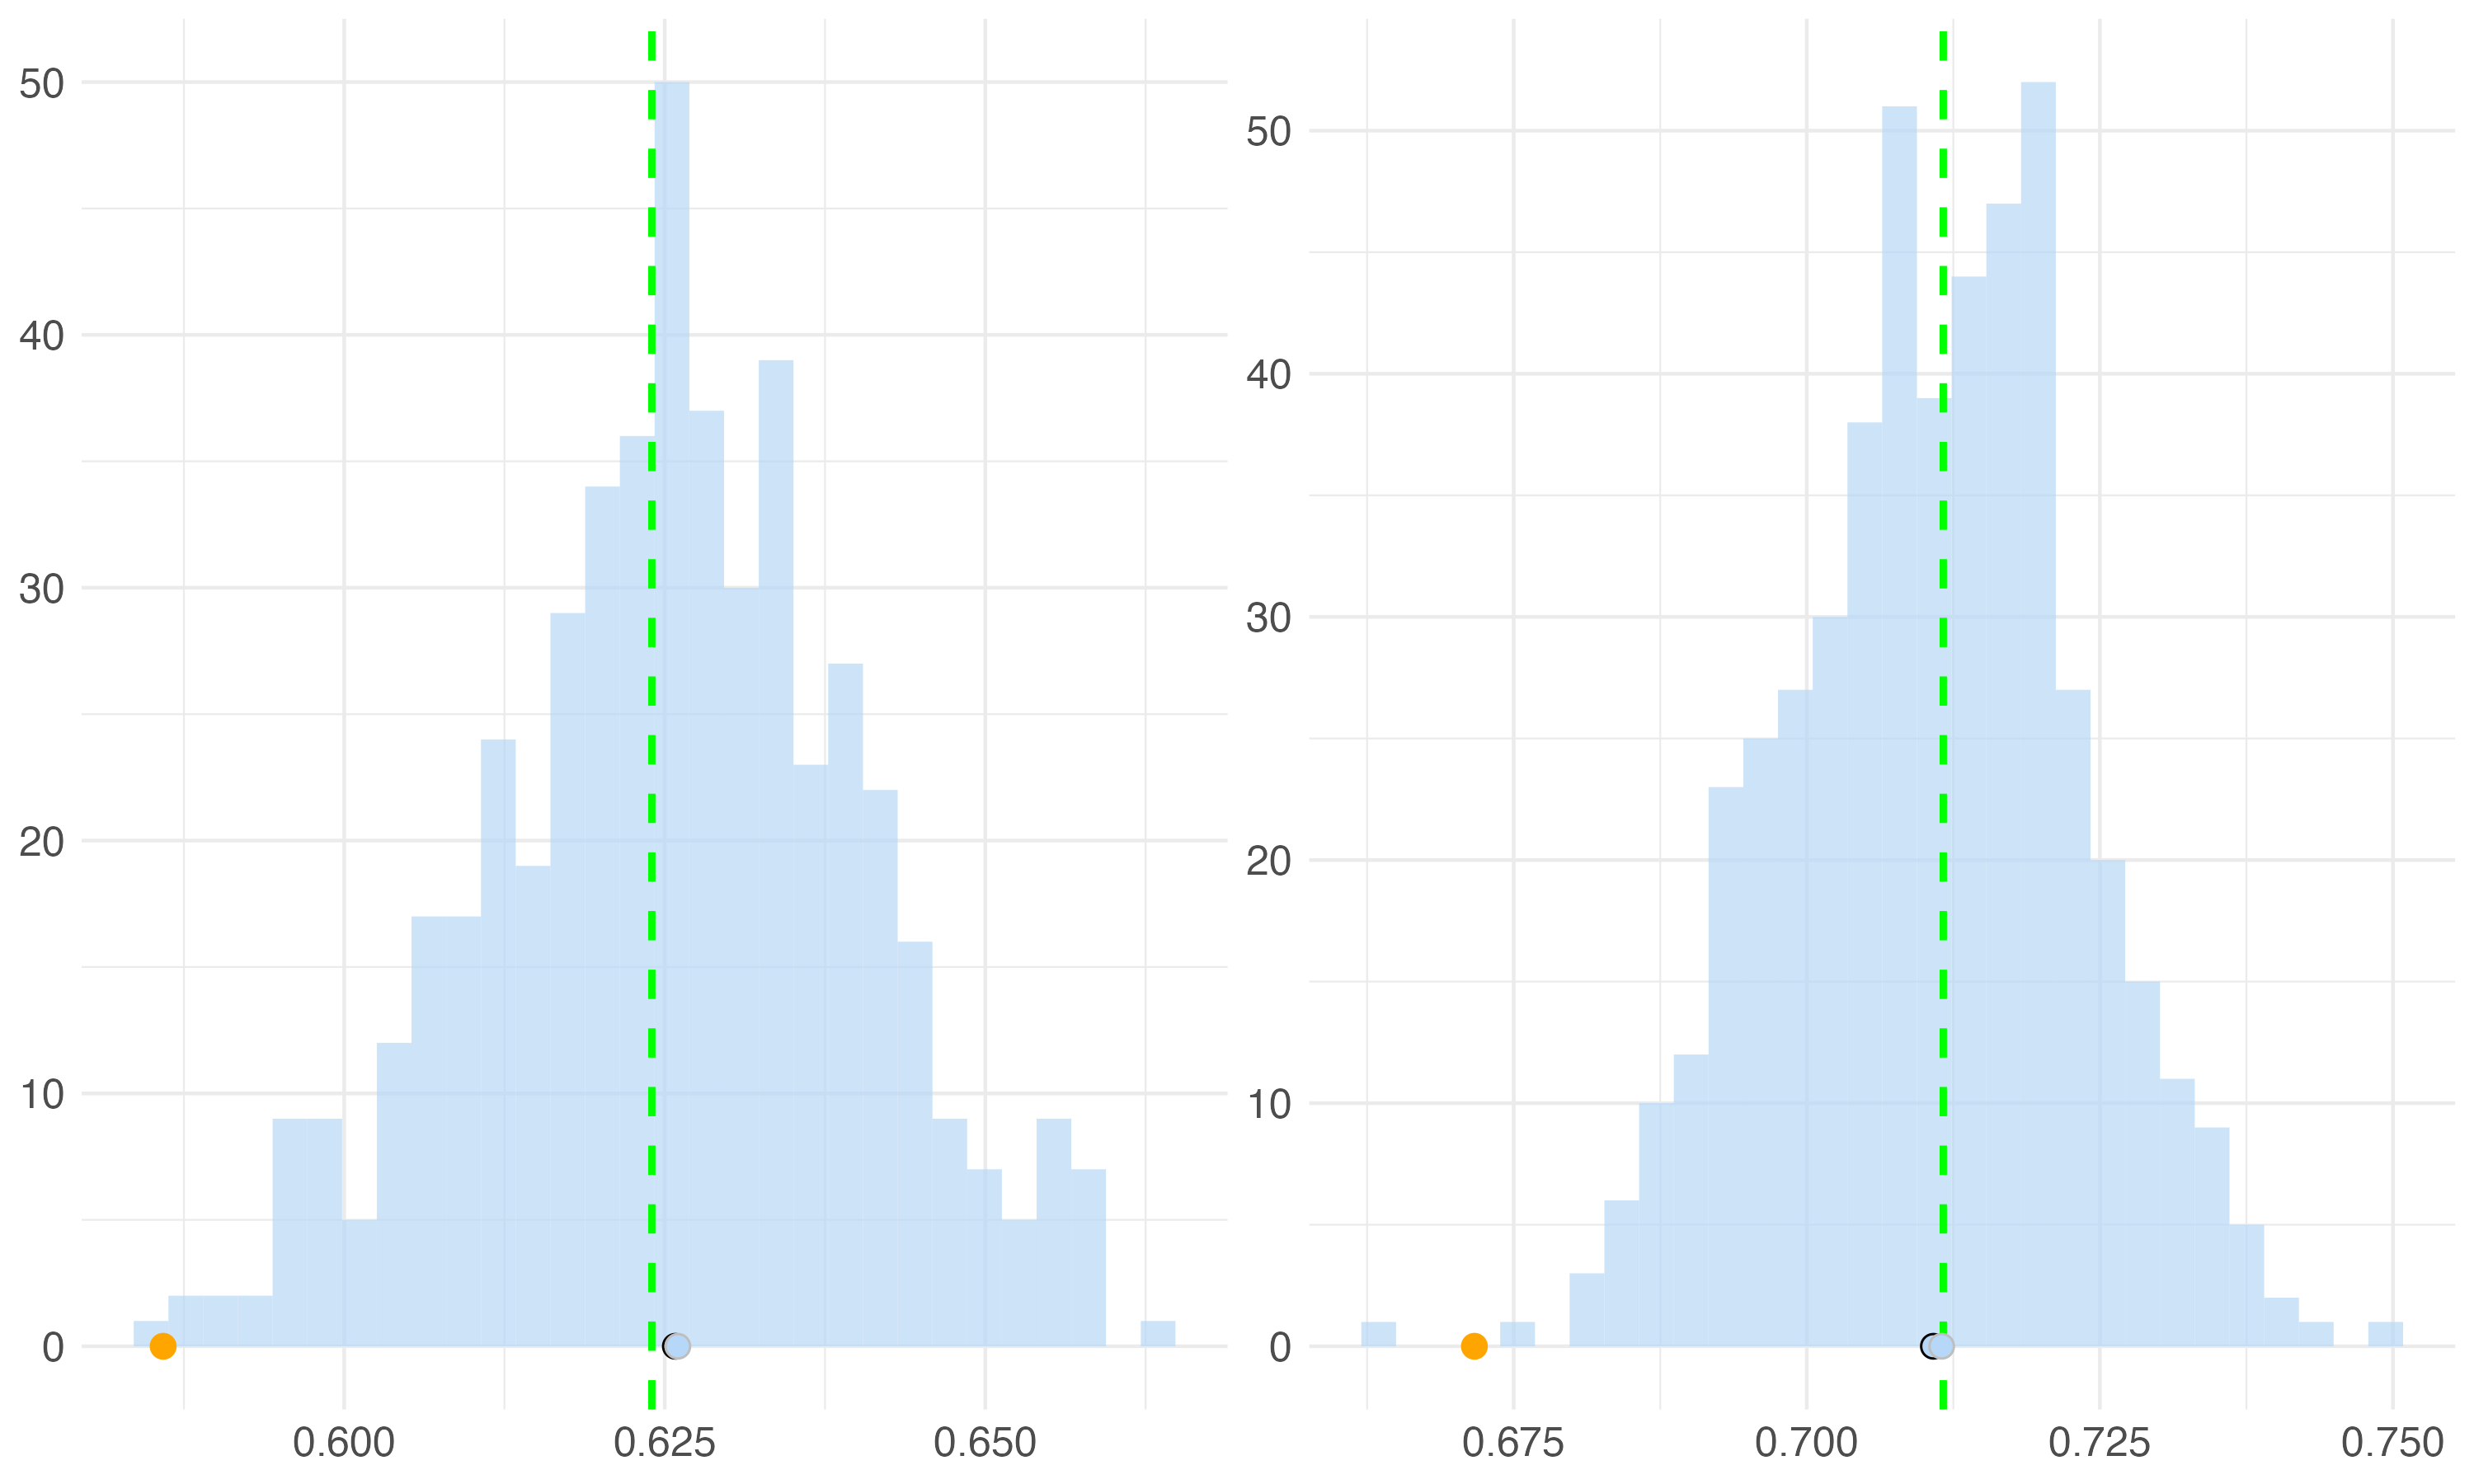
\includegraphics[width=1\linewidth]{Figures/Simulation study/R2_logit_low_pos.png}
%   \caption{(d) Marginal and conditional $R^2$ estimates for $\rho=0.1$.}
%   \label{fig:r2_logit_low_pos}
% \end{figure}
% \begin{figure}[H]\ContinuedFloat
%   \centering
%   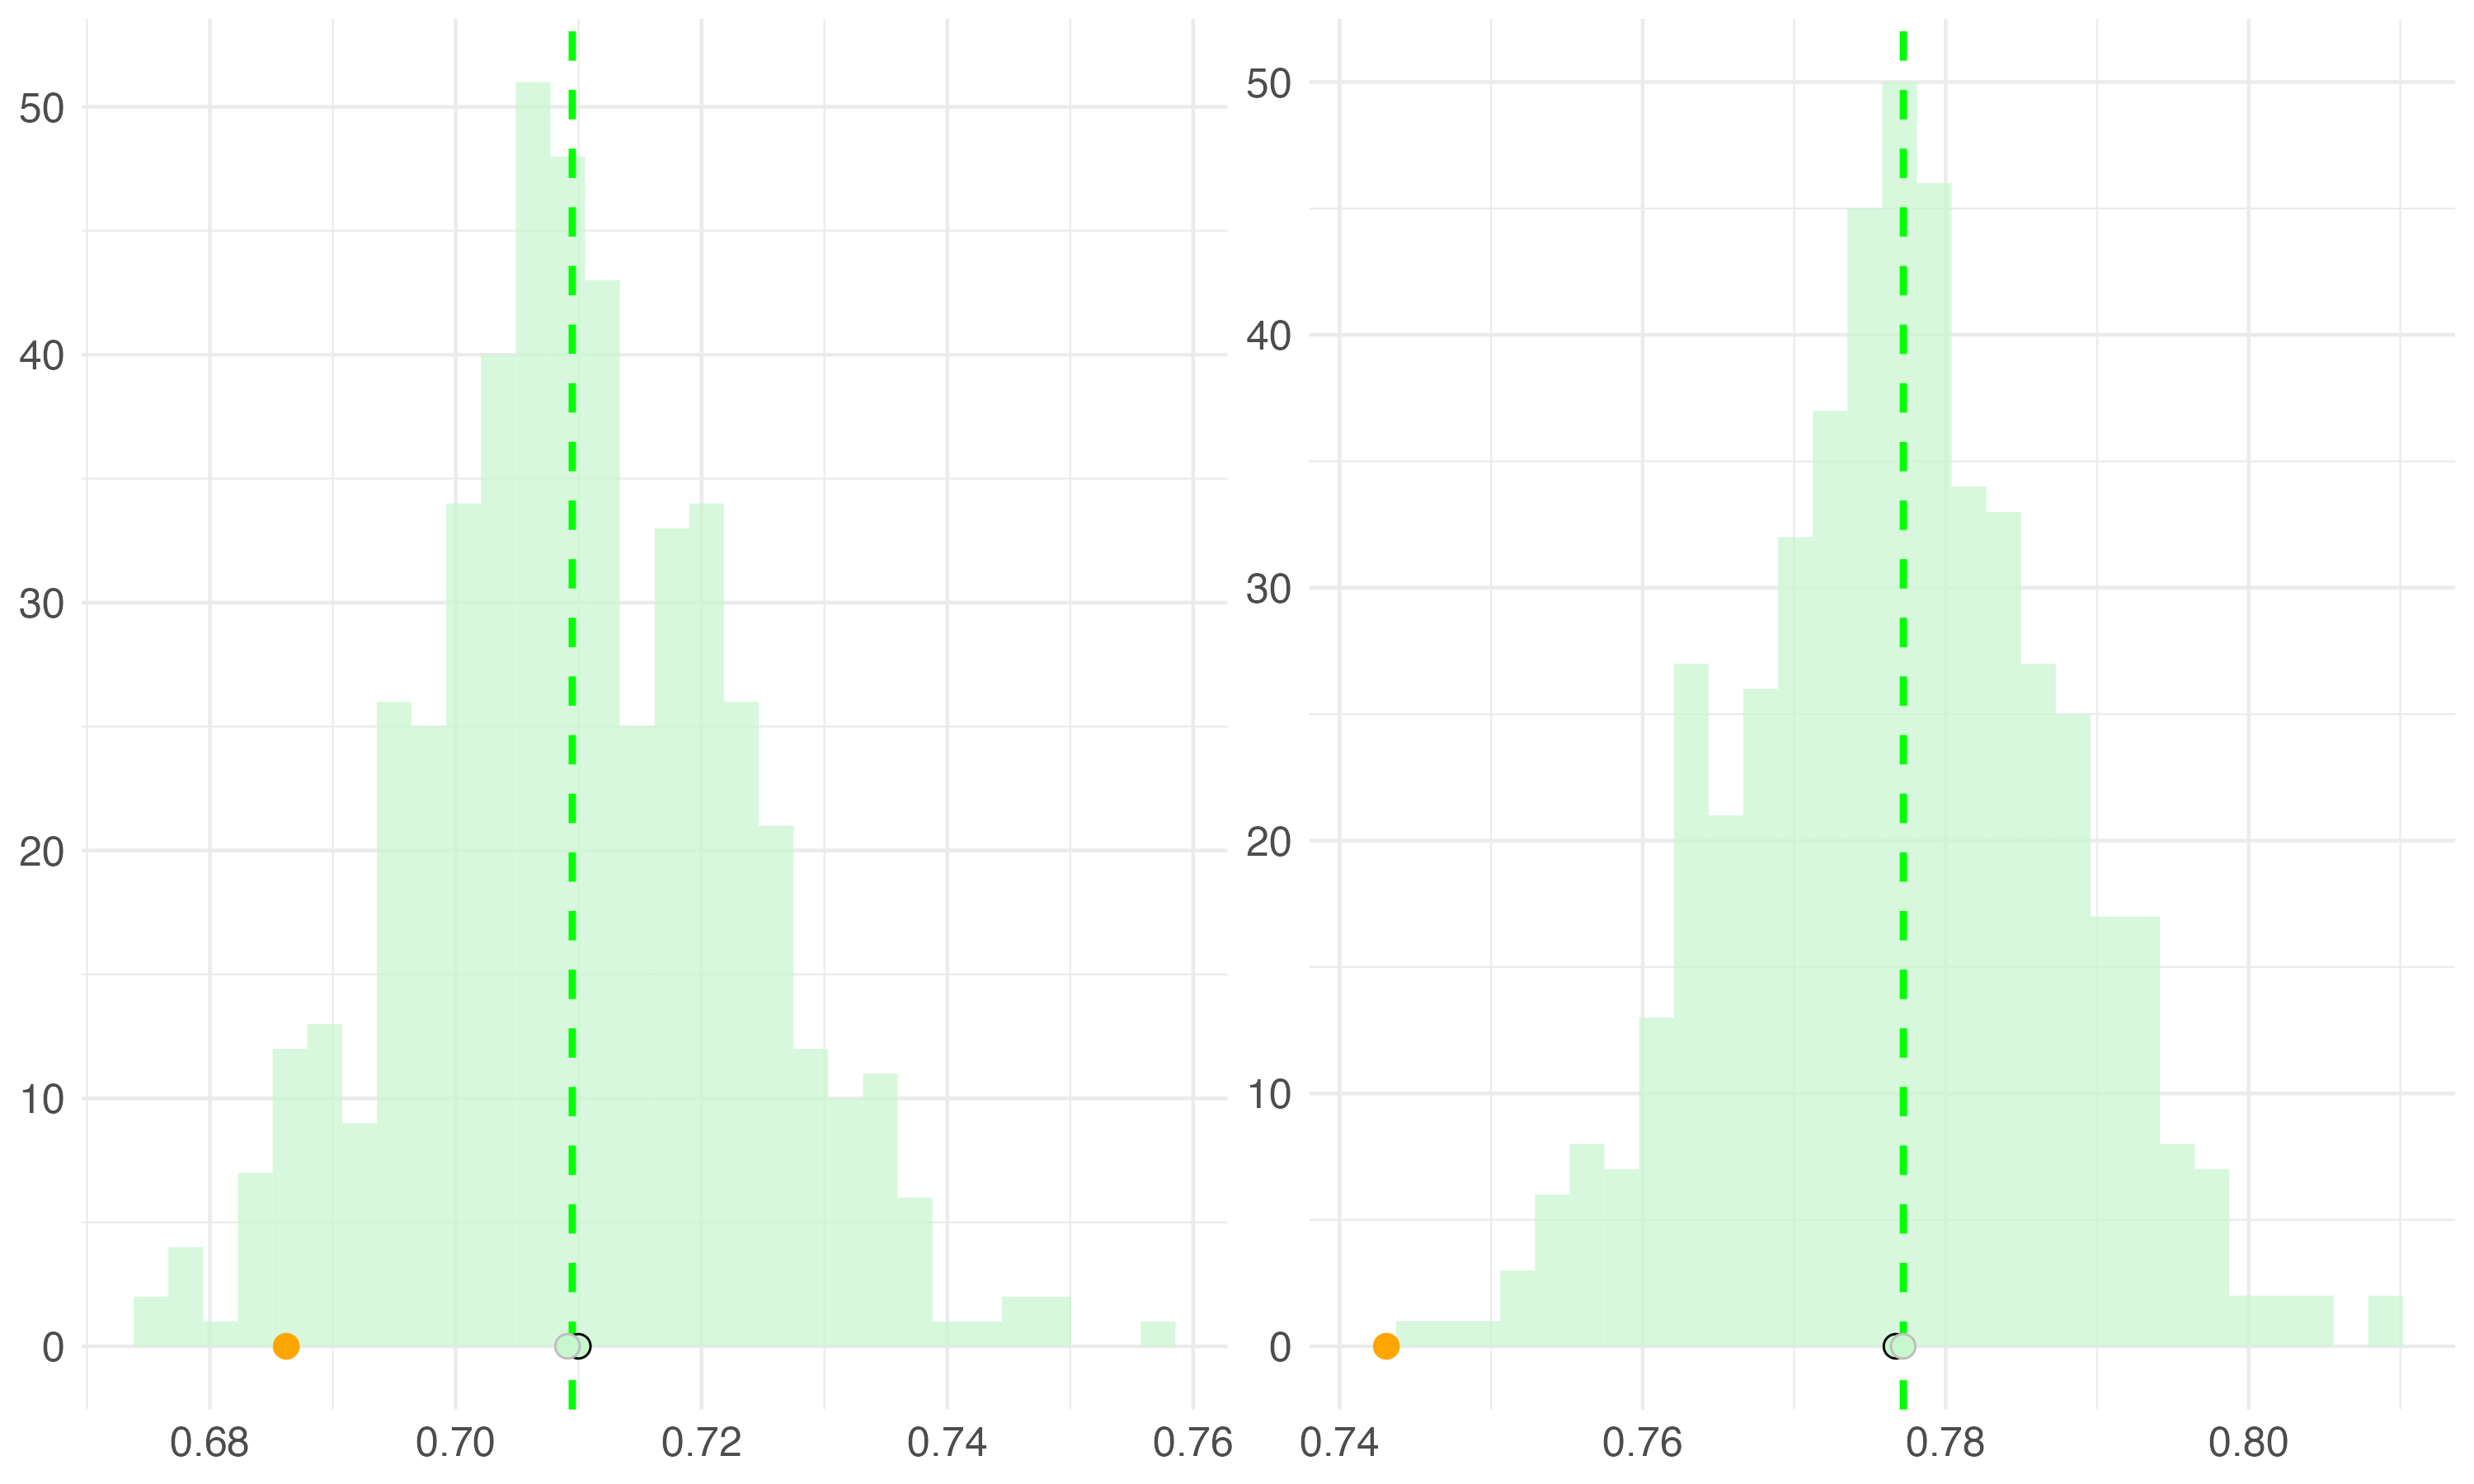
\includegraphics[width=1\linewidth]{Figures/Simulation study/R2_logit_high_pos.png}
%   \caption{(e) Marginal and conditional $R^2$ estimates for $\rho=0.4$.}
%   \label{fig:r2_logit_high_pos}
% \end{figure}
\begin{figure}[H]
  \centering
  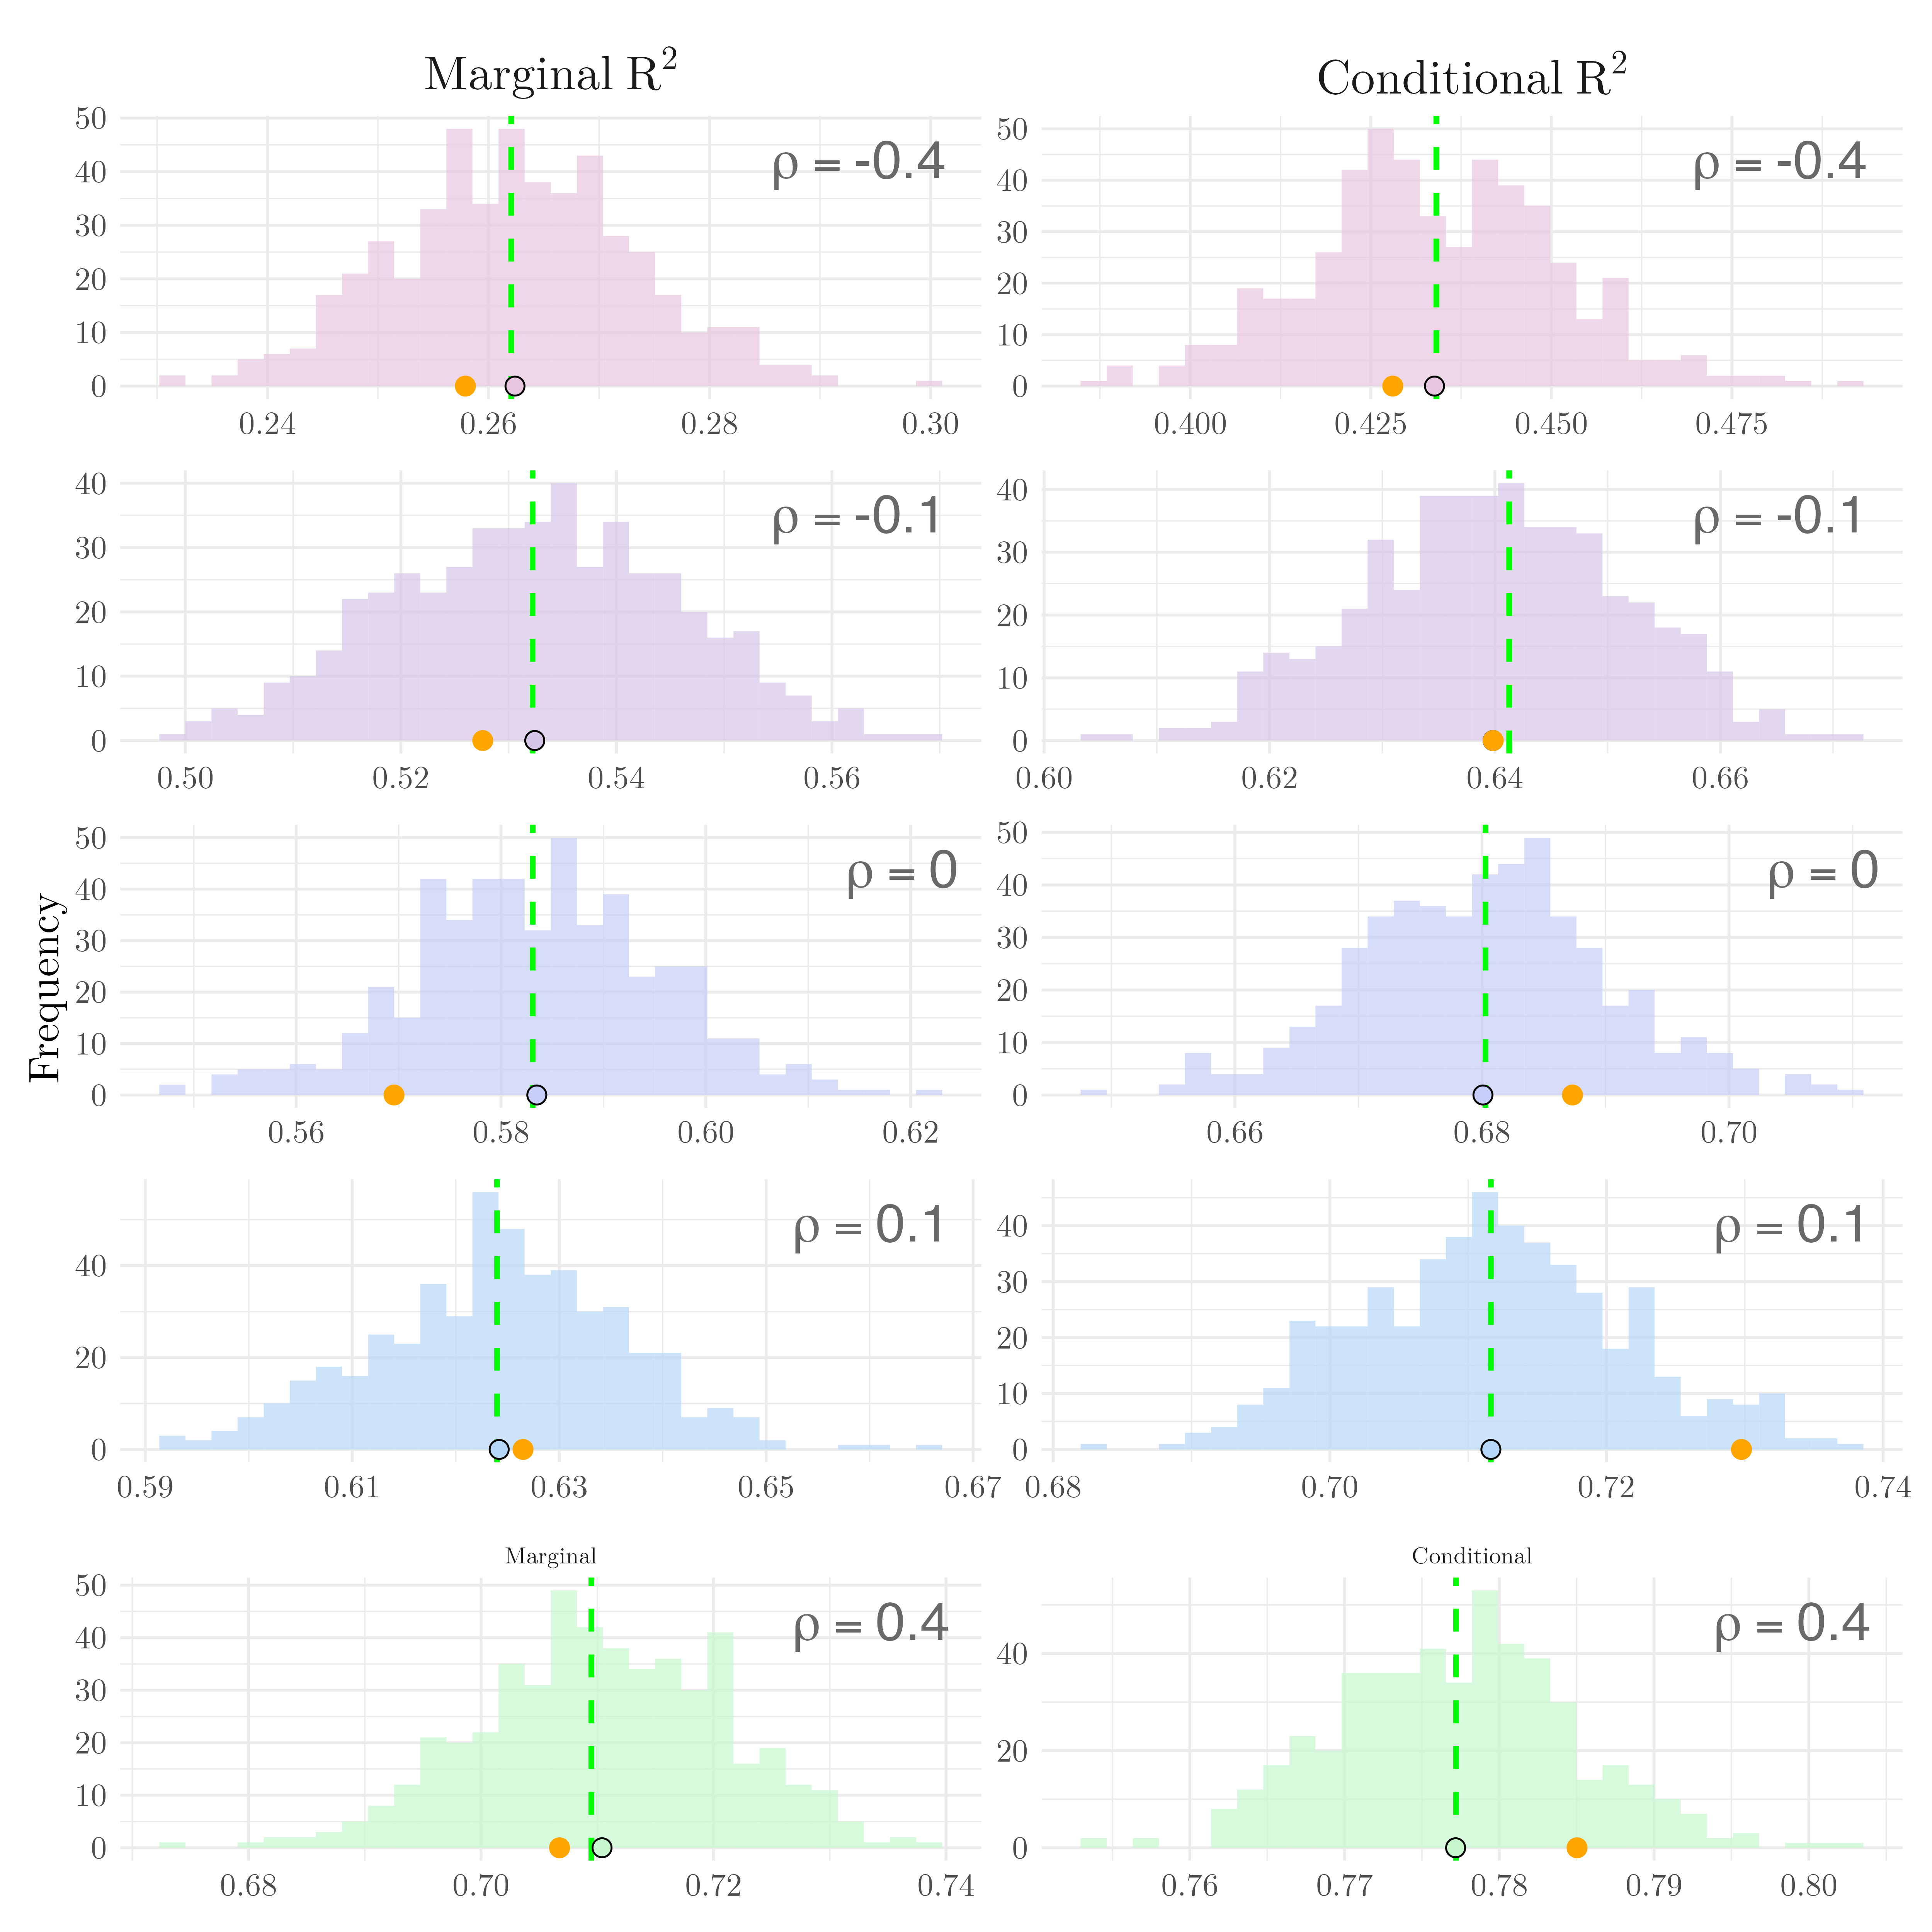
\includegraphics[width=1.1\linewidth]{Figures/Simulation study/R2_combined_logit.png}
  \caption[Marginal and conditional $R^2$ in binomial GLMM]{Histograms with the posterior modes of the estimated marginal and conditional $R^2$ from the BVI method for the binomial regression for the different correlation levels $\rho$. The posterior modes are calculated by the Bayesian Variable Importance method from the $N_{\text{sim}}=500$ simulations in the simulation study. The expected values are displayed as vertical green lines, and can be found in \Cref{table:r2values}, while the orange dot denotes the estimate from the \texttt{rptR} package. The mean value of the $R^2$ modes for all simulations is marked with a circle at the bottom of each histogram.}
  \label{fig:r2_combined_logit}
\end{figure}

\subsection{Poisson simulation}
The second model fit in the simulation study is a Poisson regression with log-link. The Poisson models were fit with the same correlation levels as the binomial simulation and $N_{\text{sim}}=500$ models for each level were fitted. For each fitted model, the Bayesian Variable Importance method extracts the posterior mode and then calculates the relative variable importance measures as described in \Cref{ch:method}. In the supplementary material (\Cref{ap:supplementary}, see \Cref{table:summary_poisson}), a summary of the mean and $95\%$ quantile values of the $500$ importance estimates for different correlation levels is displayed.
\subsubsection{Fixed effects}
As for the binomial model, we first look at the fixed effects. The estimates of posterior modes for relative importance for the fixed effects (\Cref{fig:fixed_combined_poisson}) are very similar in shape as the binomial model. Again, the spread is somewhat varying for the different correlation levels. Overall, the estimates for the Poisson model are marginally larger than the binomial for negative correlations, and marginally smaller for positive correlations. This is mainly due to the log-link having a distributional variance which is dependent on the correlation of covariates, and the logit-link having a constant distributional variance. When covariates are negatively correlated, the distributional variance of the log-link decreases and the importance allocated to covariates increases. Similarily, the opposite happens when covariates are positively correlated. The quantiles of the Poisson model is marginally more narrow than that of the binomial model. It seems the estimates form a normal curve about the mean, and for $\rho=0$ the average estimated importance is close to the expected value. The same influence of varying correlation levels can be seen as in the binomial model, namely that we obtain larger importance of the fixed effects when the correlation increases. Again the difference is notably large, with the average relative importance of $X_1$ going from $0.017$ for $\rho=-0.4$ to $0.181$ for $\rho=0.4$. For $X_2$ and $X_3$ the average relative importance for the same correlation levels increases from $0.066$ to $0.251$ and from $0.143$ to $0.314$ respectively.
\\
\\
Further, we see the same pattern of larger increase in importance to $X_1$ than for $X_2$ and larger for $X_2$ than $X_3$, as for the binomial model, when correlation increases from $\rho=0$ to $\rho=0.4$. Specifically, $X_1$ increases with $0.084$, $X_2$ with $0.058$ and $X_3$ with $0.024$ when we go from uncorrelated covariates to the highest correlation level. This is in line with our expectations, as the diagonal elements of $\boldsymbol{\Lambda}$ decrease with increasing correlation levels and the off-diagonal elements increase. The inverse pattern is once again not so clear, as the decrease of $X_3$ is larger than the decrease of $X_1$ and $X_2$. However, if one looks at the relative decrease in importance, it is clear that the decrease is larger for $X_1$ and $X_2$ than for $X_3$ when going from $\rho=0$ to $\rho=-0.4$. The inverse pattern may therefore be hard to detect, due to the relatively large difference in magnitude of the coefficients. For the case $\rho=0$, we see that the mean of our samples coincides with the expected relative importance (\Cref{table:3}), and it seems the model express the expected pattern of relative importance for varying correlation levels.
% \newline
% \newline
% It is apparent that for the case $\rho=0.4$, the distribution of relative importance of all covariates contains values very close to zero. After some investigation of the fitted models, it turns out that INLA sometimes returns a model that estimates all fixed coefficients to be $0$, but estimates the random effect almost as expected. One might expect that such a model is not sensible and that a model fit should not have been possible. However, it seems that the models are fit and therefore the resulting variable importance measures have been included in results of the simulation study. With the coefficients estimated to be close to zero, the model will consequently estimate the relative importance of the fixed effects close to zero. It is therefore plausible to believe that the method correctly estimates relative importance, and that this model fit might be caused by some problem with the simulated dataset or INLA.
% \begin{figure}[H]
%   \centering
%   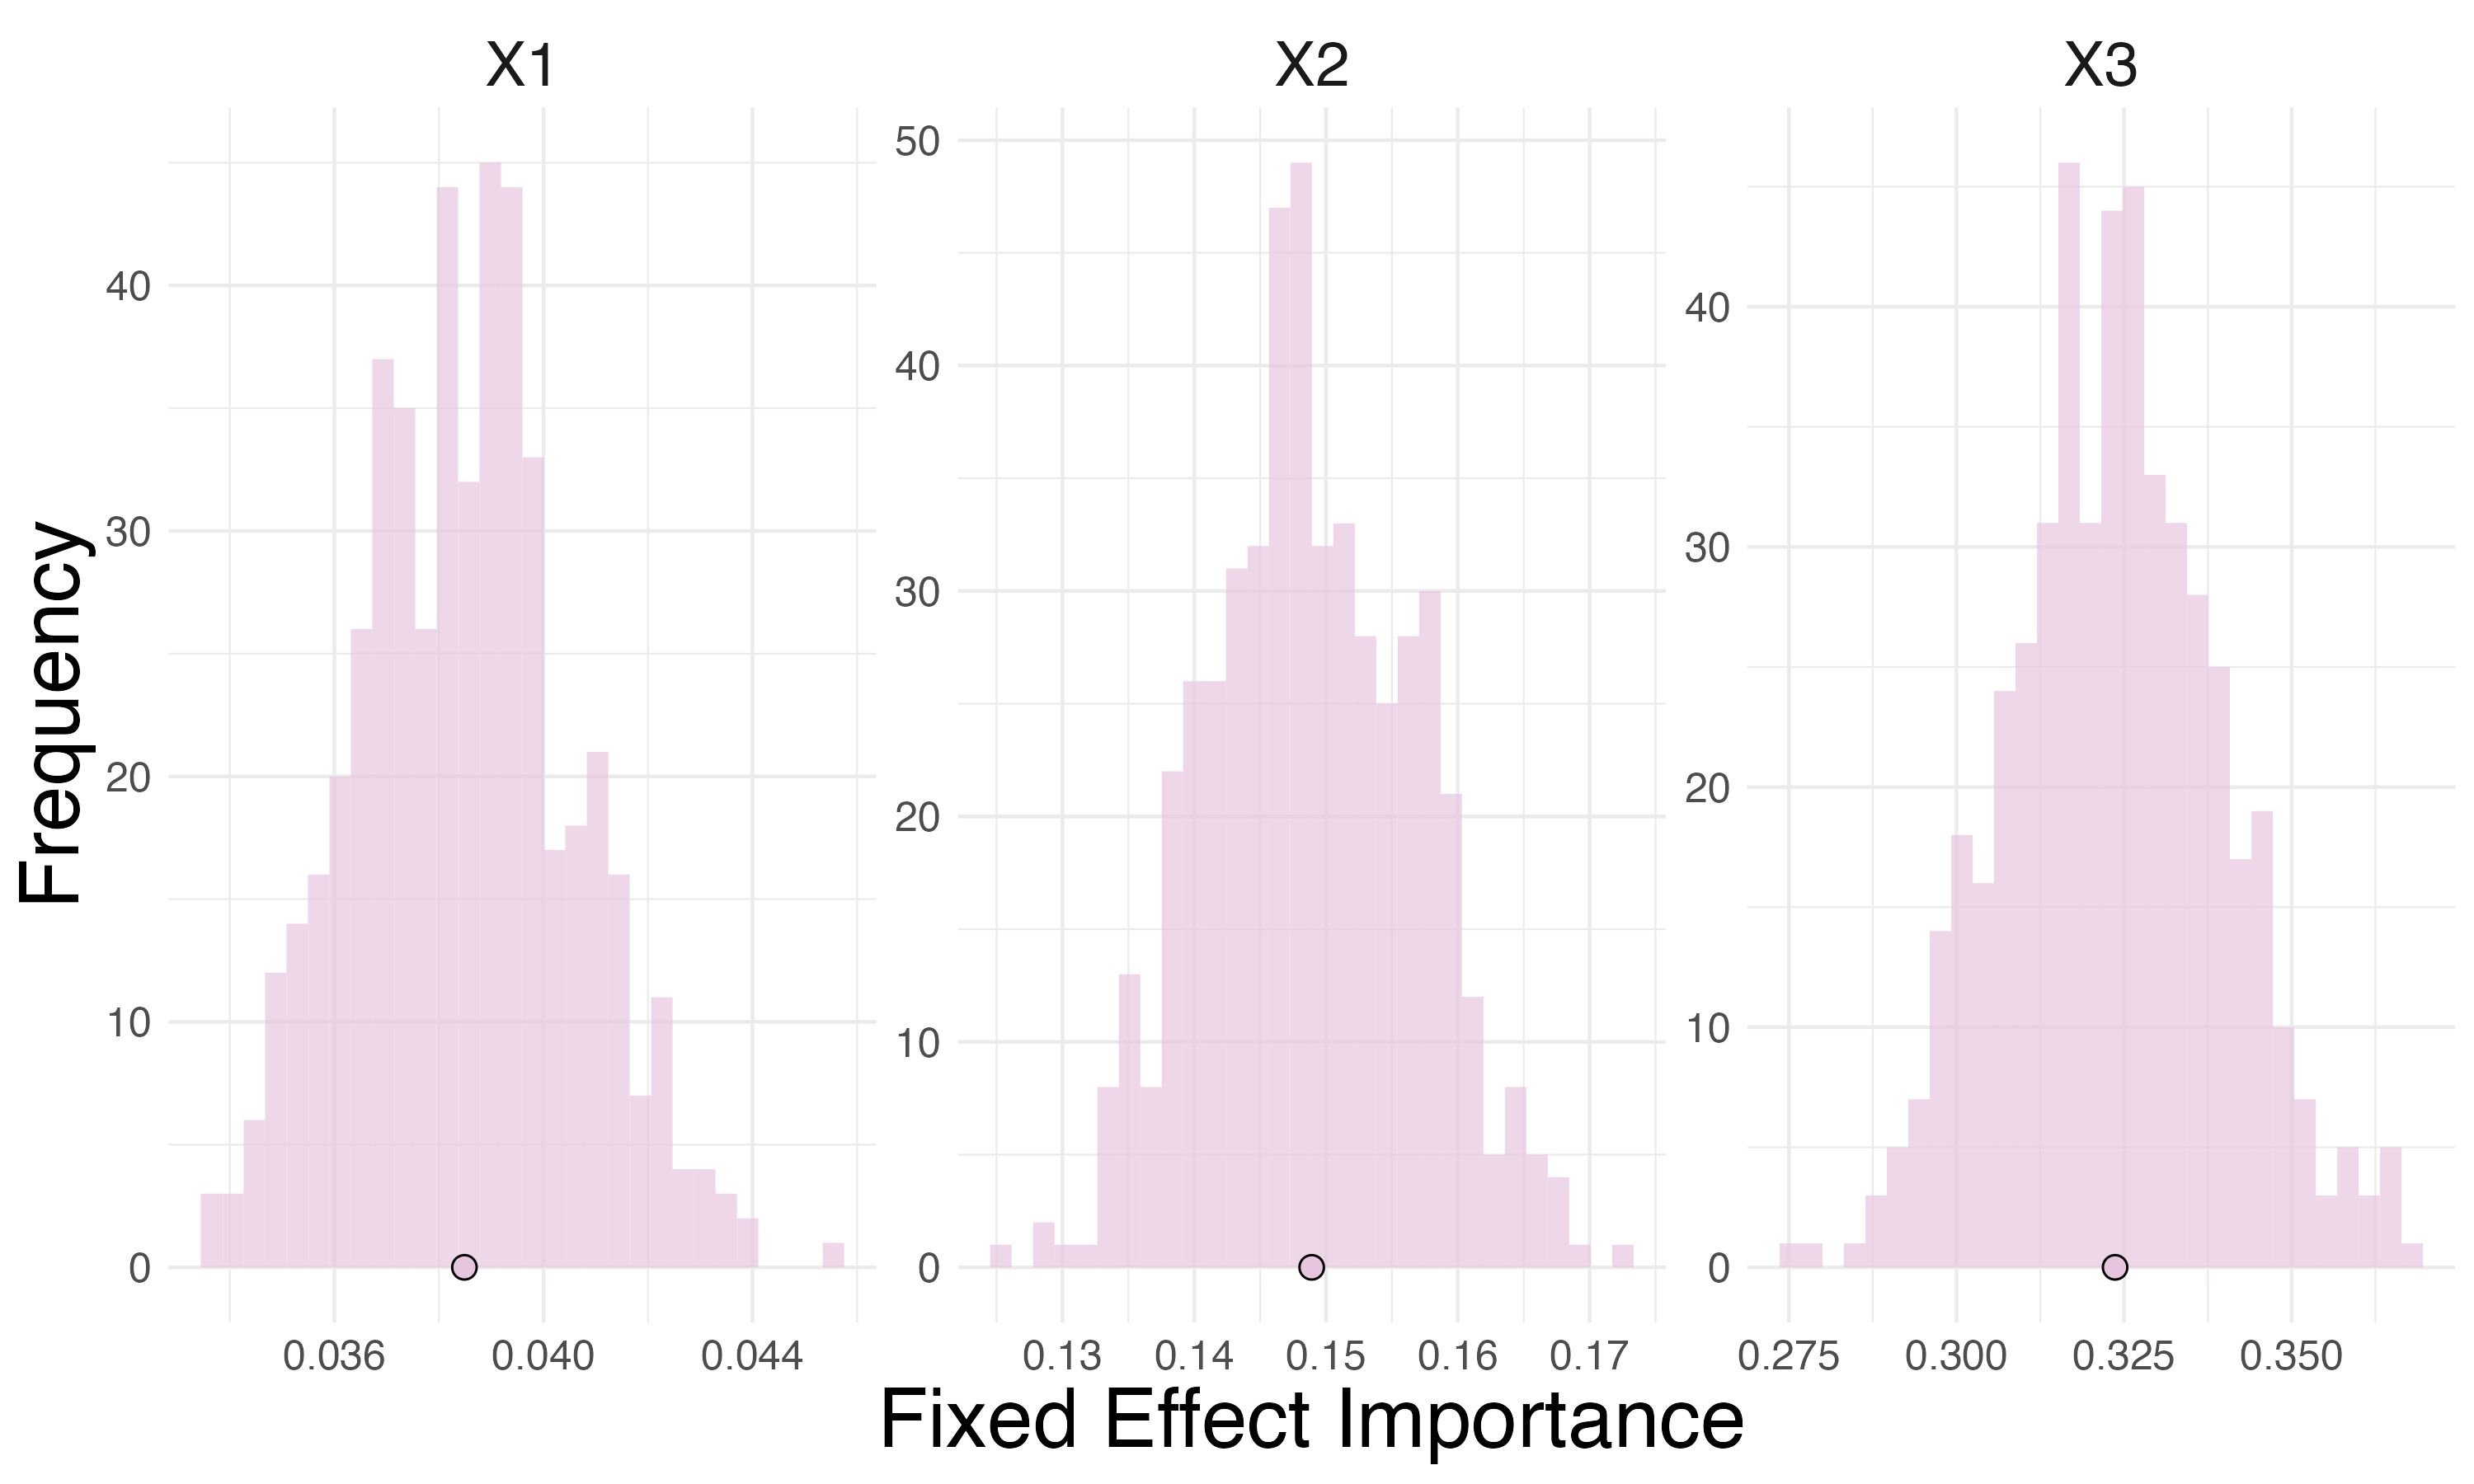
\includegraphics[width=1\linewidth]{Figures/Simulation study/Fixed_high_neg_poisson.png}
%   \caption{Histogram with relative importance estimates for the fixed effects in the Poisson regression with different correlation levels $\rho$. The values are estimated from $N_{\text{sim}}=500$ simulations by the Bayesian Variable Importance method in the simulation study. The regression coefficients are set to be  $\boldsymbol{\beta}=(1, \sqrt{2}, \sqrt{3})^T$ and the vertical green line in (c) is the expected relative importance in the case of uncorrelated data. The mean of the relative importance for all simulations is denoted at the bottom of each histogram as a circle. (a) Relative importance of the fixed effects $\mathbf{X_1},  \mathbf{X}_2, \mathbf{X}_3$ for $\rho=-0.4$.}
%   \label{fig:fixed_effects_poisson_high_neg}
% \end{figure}
% \begin{figure}[H]\ContinuedFloat
%   \centering
%   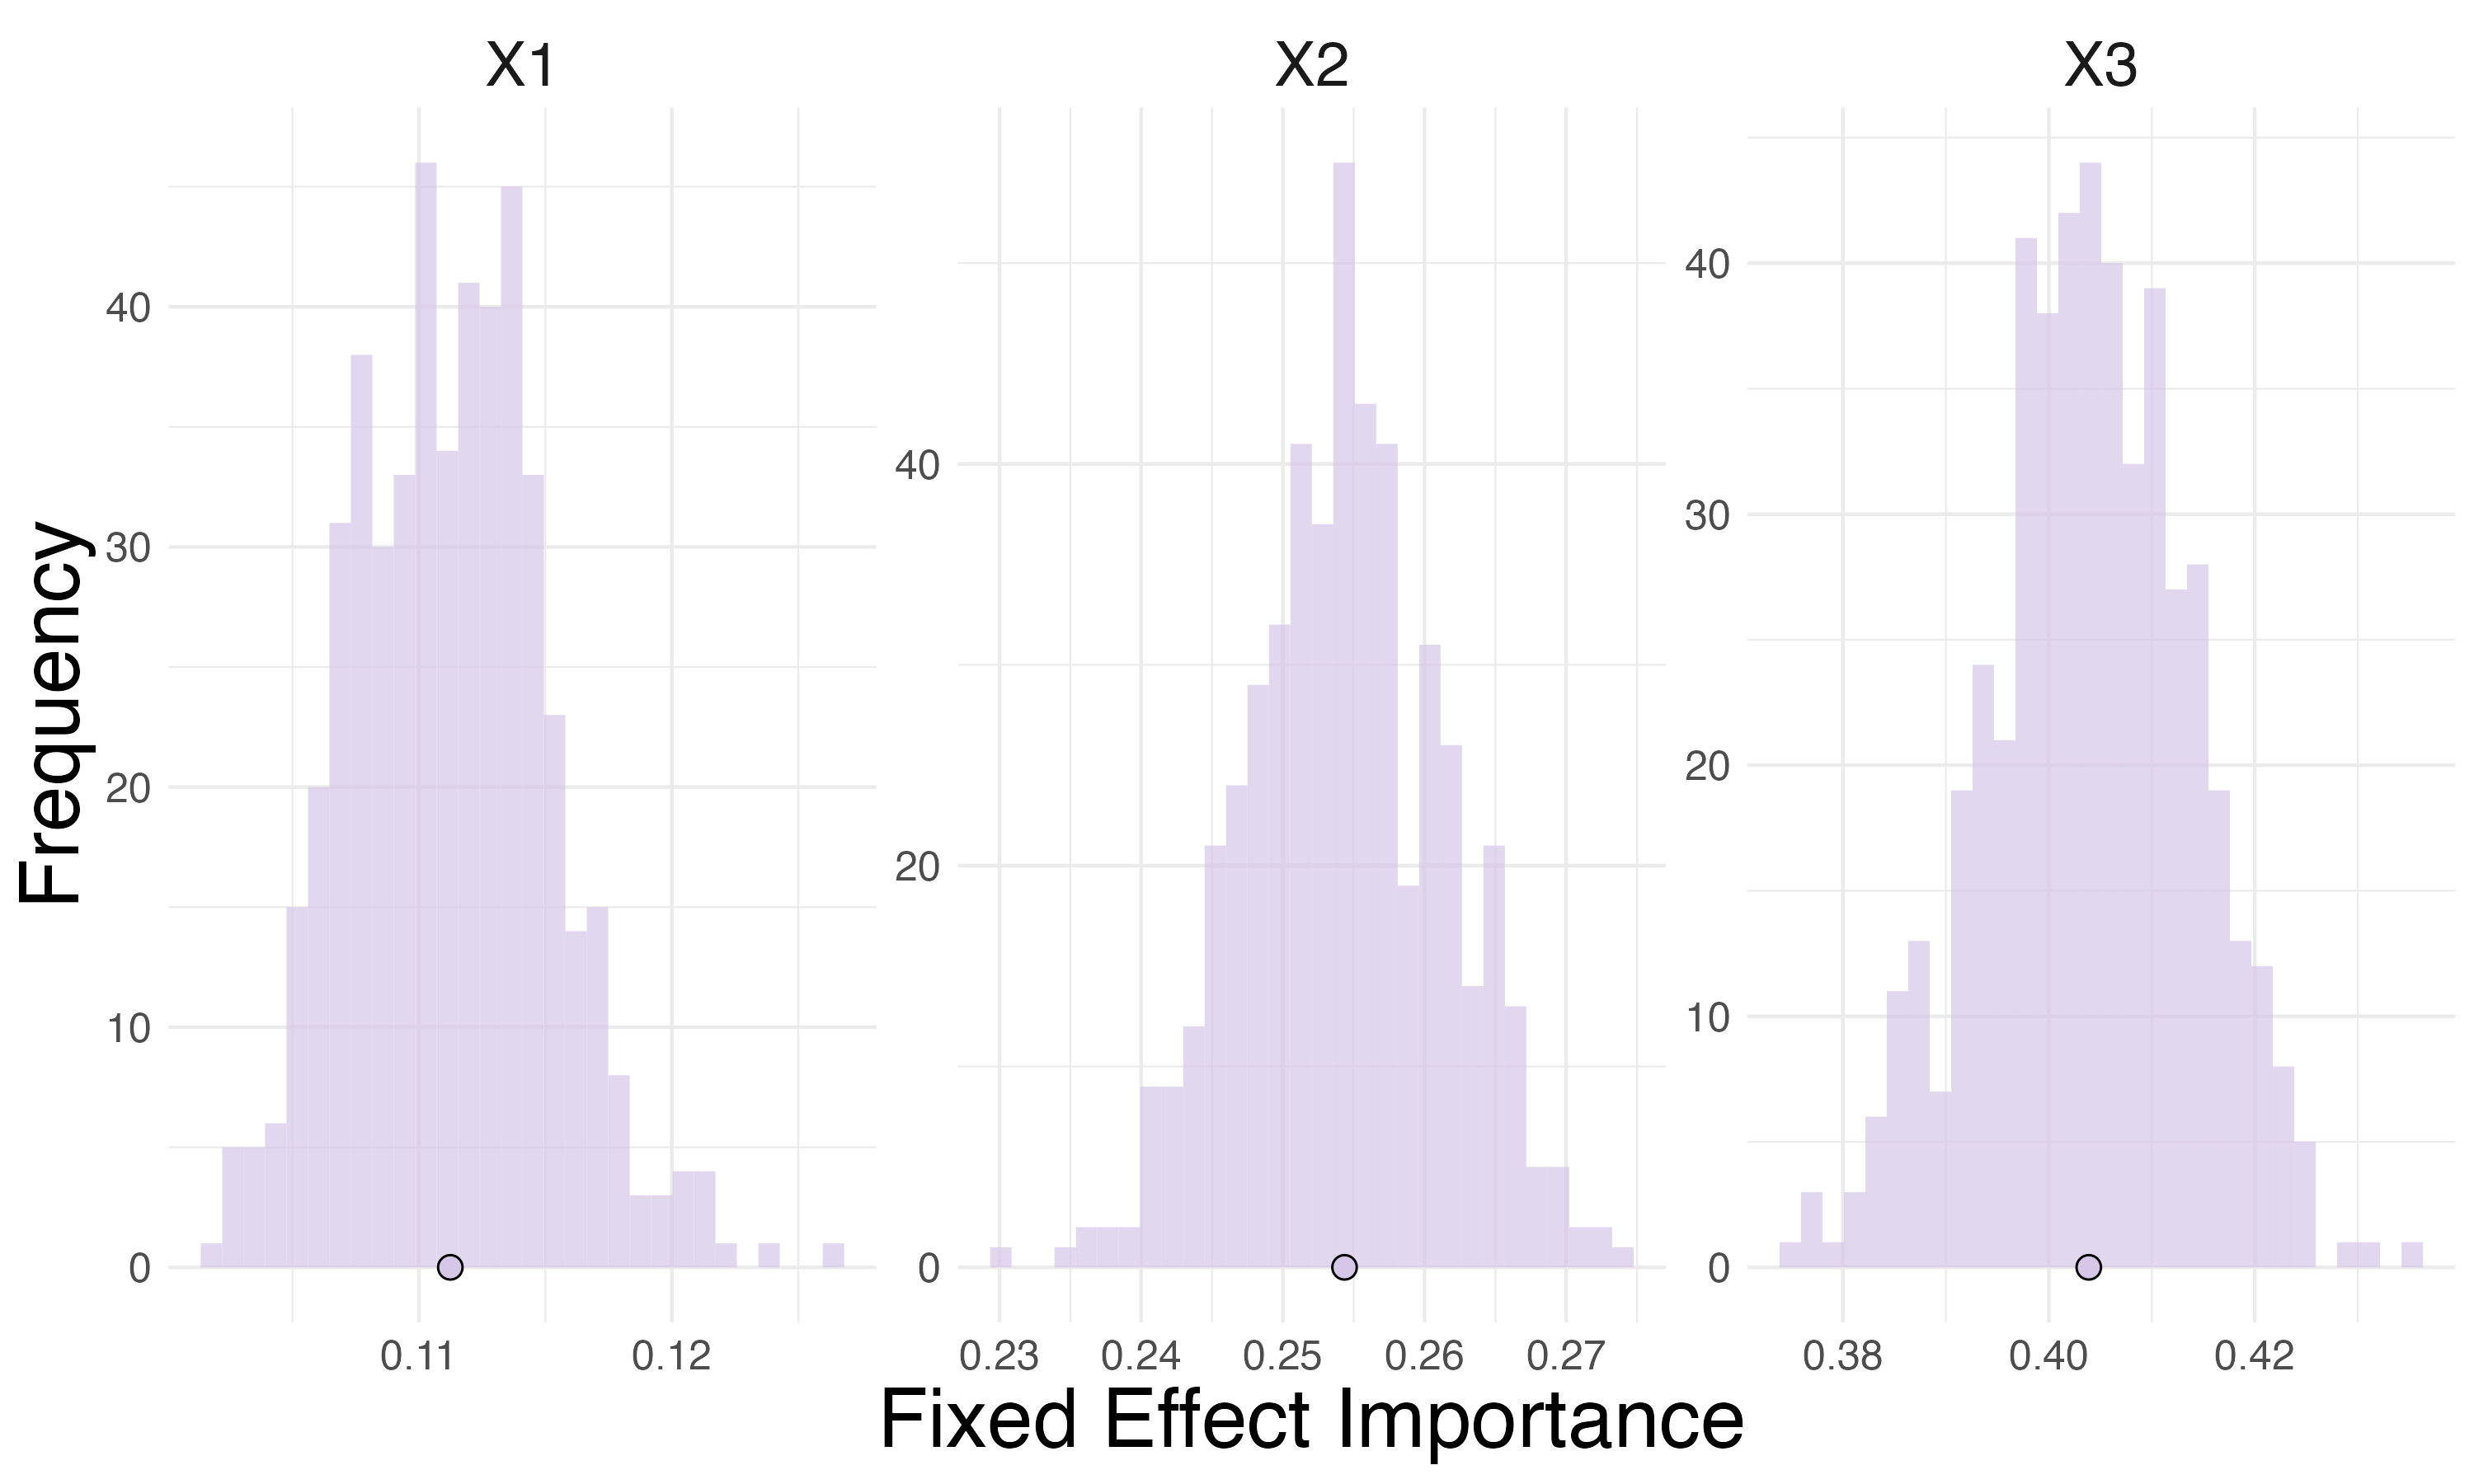
\includegraphics[width=1\linewidth]{Figures/Simulation study/Fixed_low_neg_poisson.png}
%   \caption{(b) Relative importance of the fixed effects $\mathbf{X_1},  \mathbf{X}_2, \mathbf{X}_3$ for $\rho=-0.1$.}
%   \label{fig:fixed_effects_poisson_low_neg}
% \end{figure}
% \begin{figure}[H]\ContinuedFloat
%   \centering
%   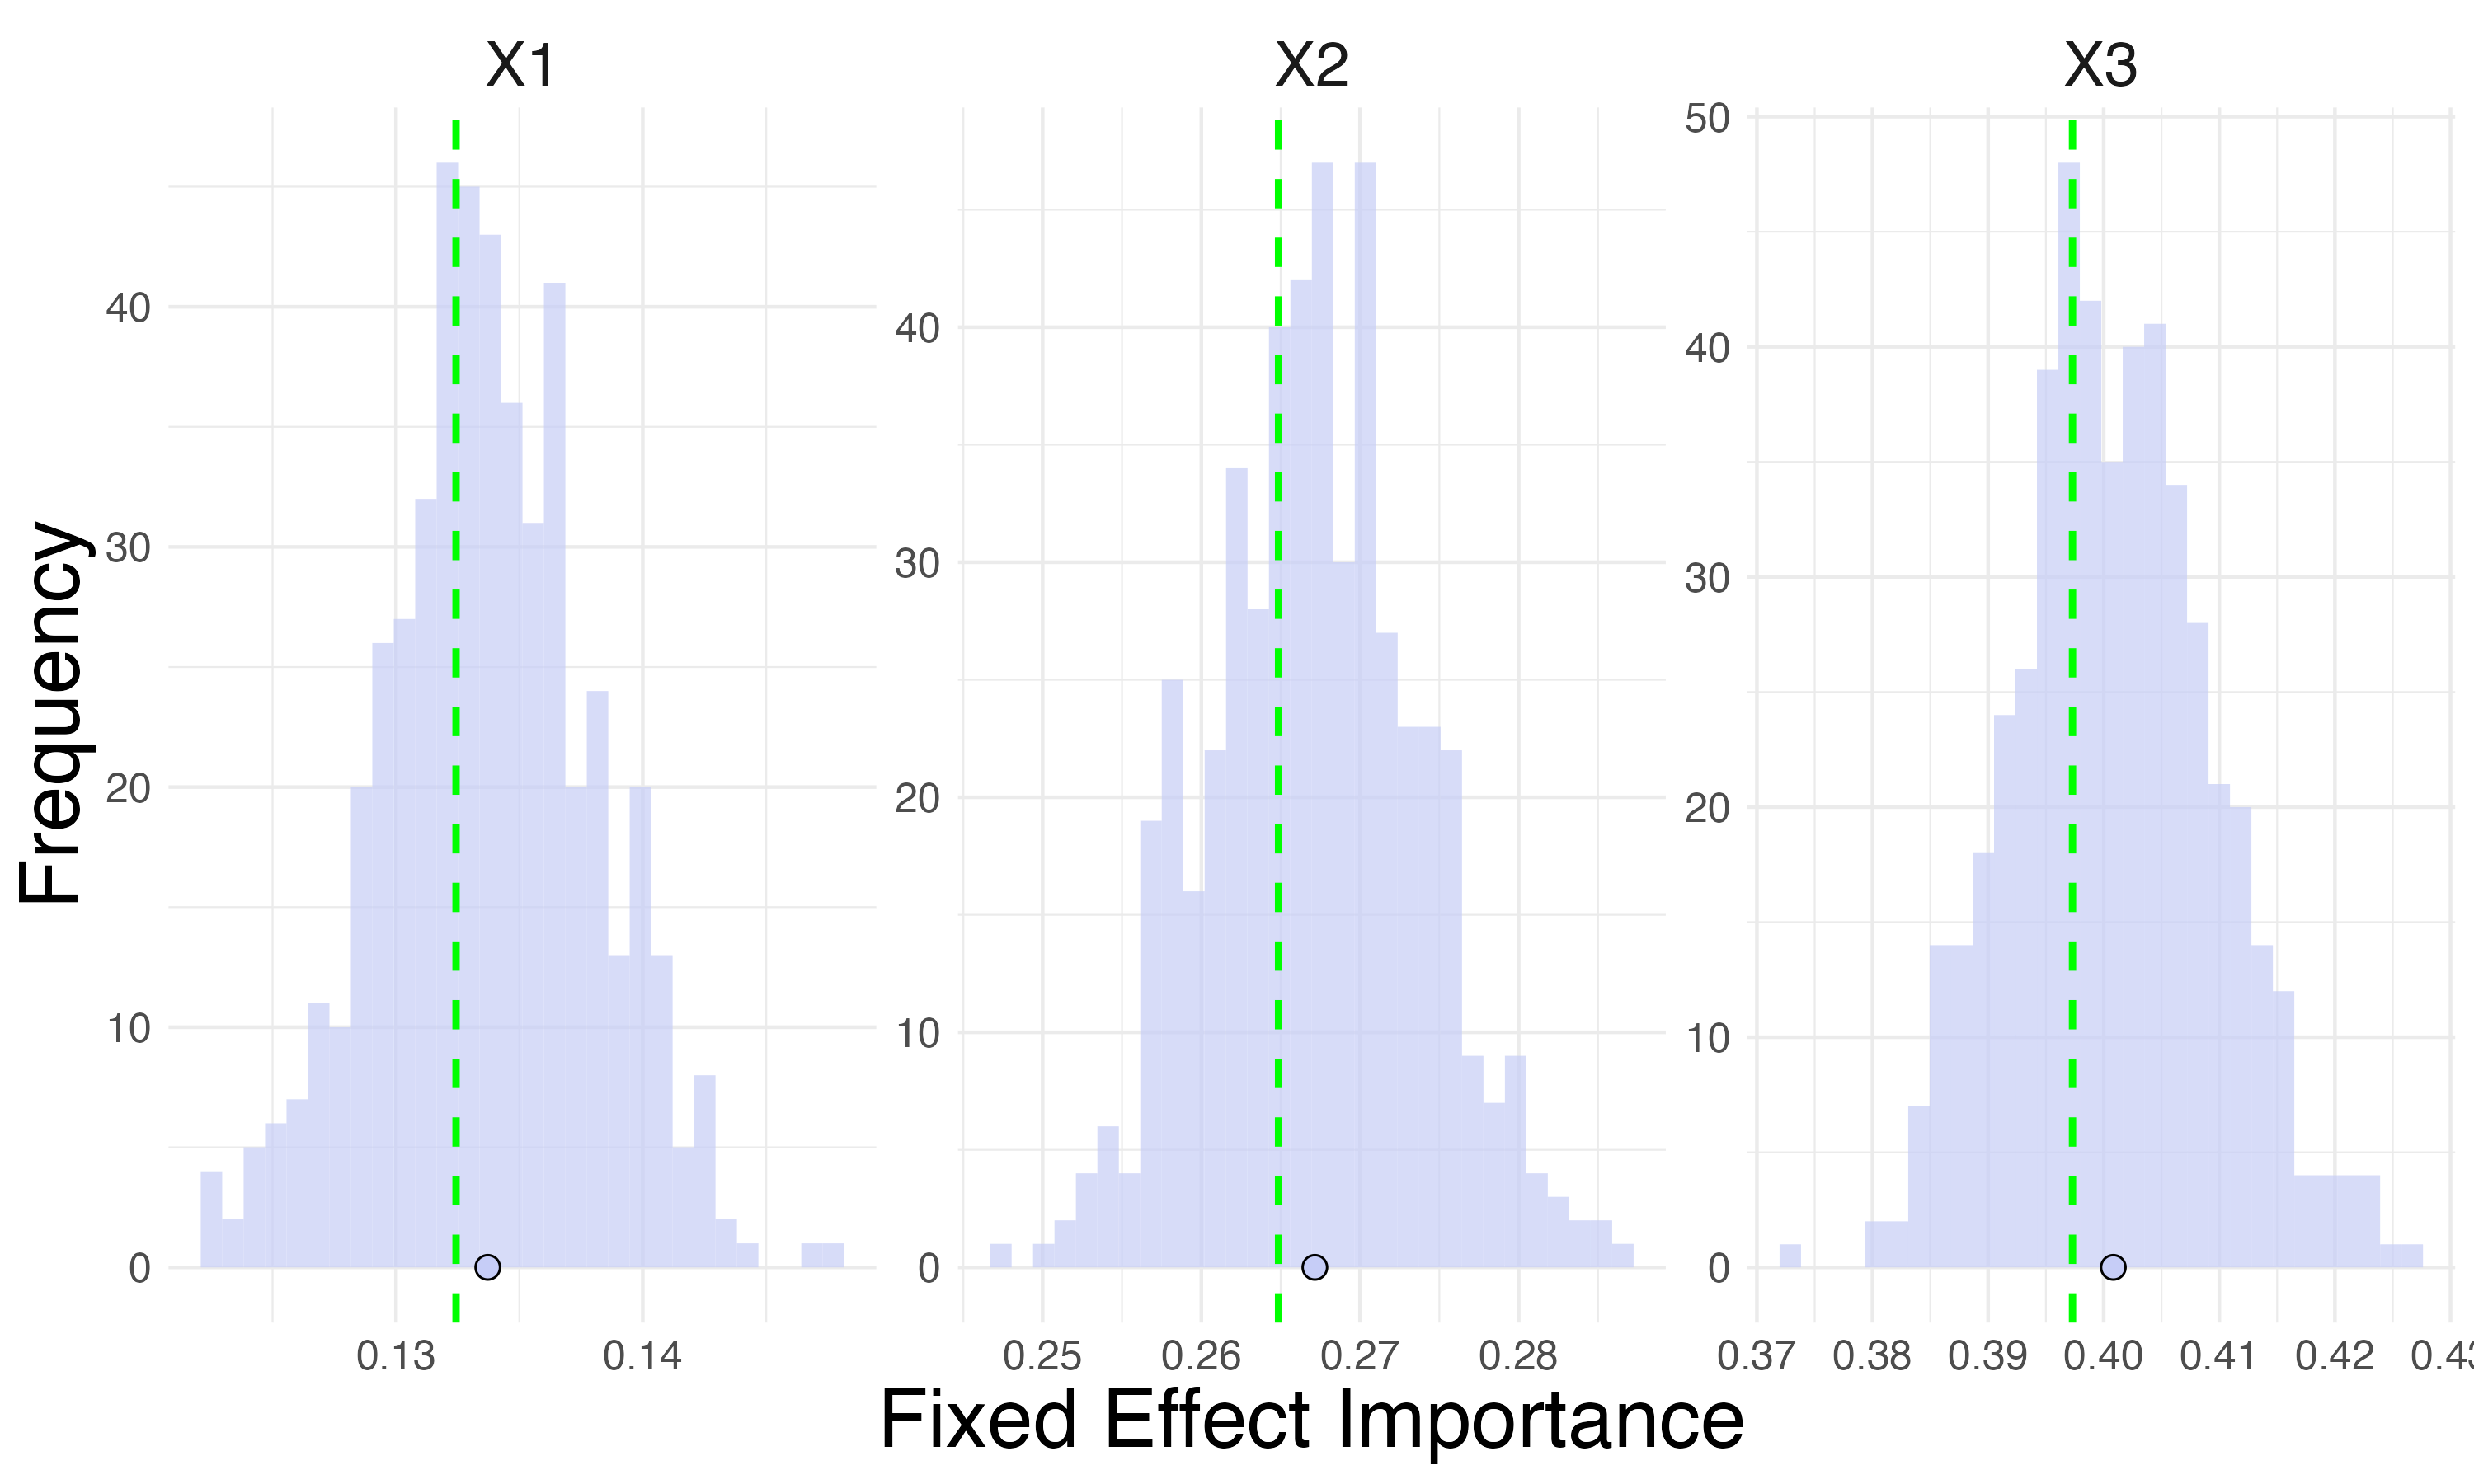
\includegraphics[width=1\linewidth]{Figures/Simulation study/Fixed_no_poisson.png}
%   \caption{(c) Relative importance of the fixed effects $\mathbf{X_1},  \mathbf{X}_2, \mathbf{X}_3$ for $\rho=0$.}
%   \label{fig:fixed_effects_poisson_no}
% \end{figure}
% \begin{figure}[H]\ContinuedFloat
%   \centering
%   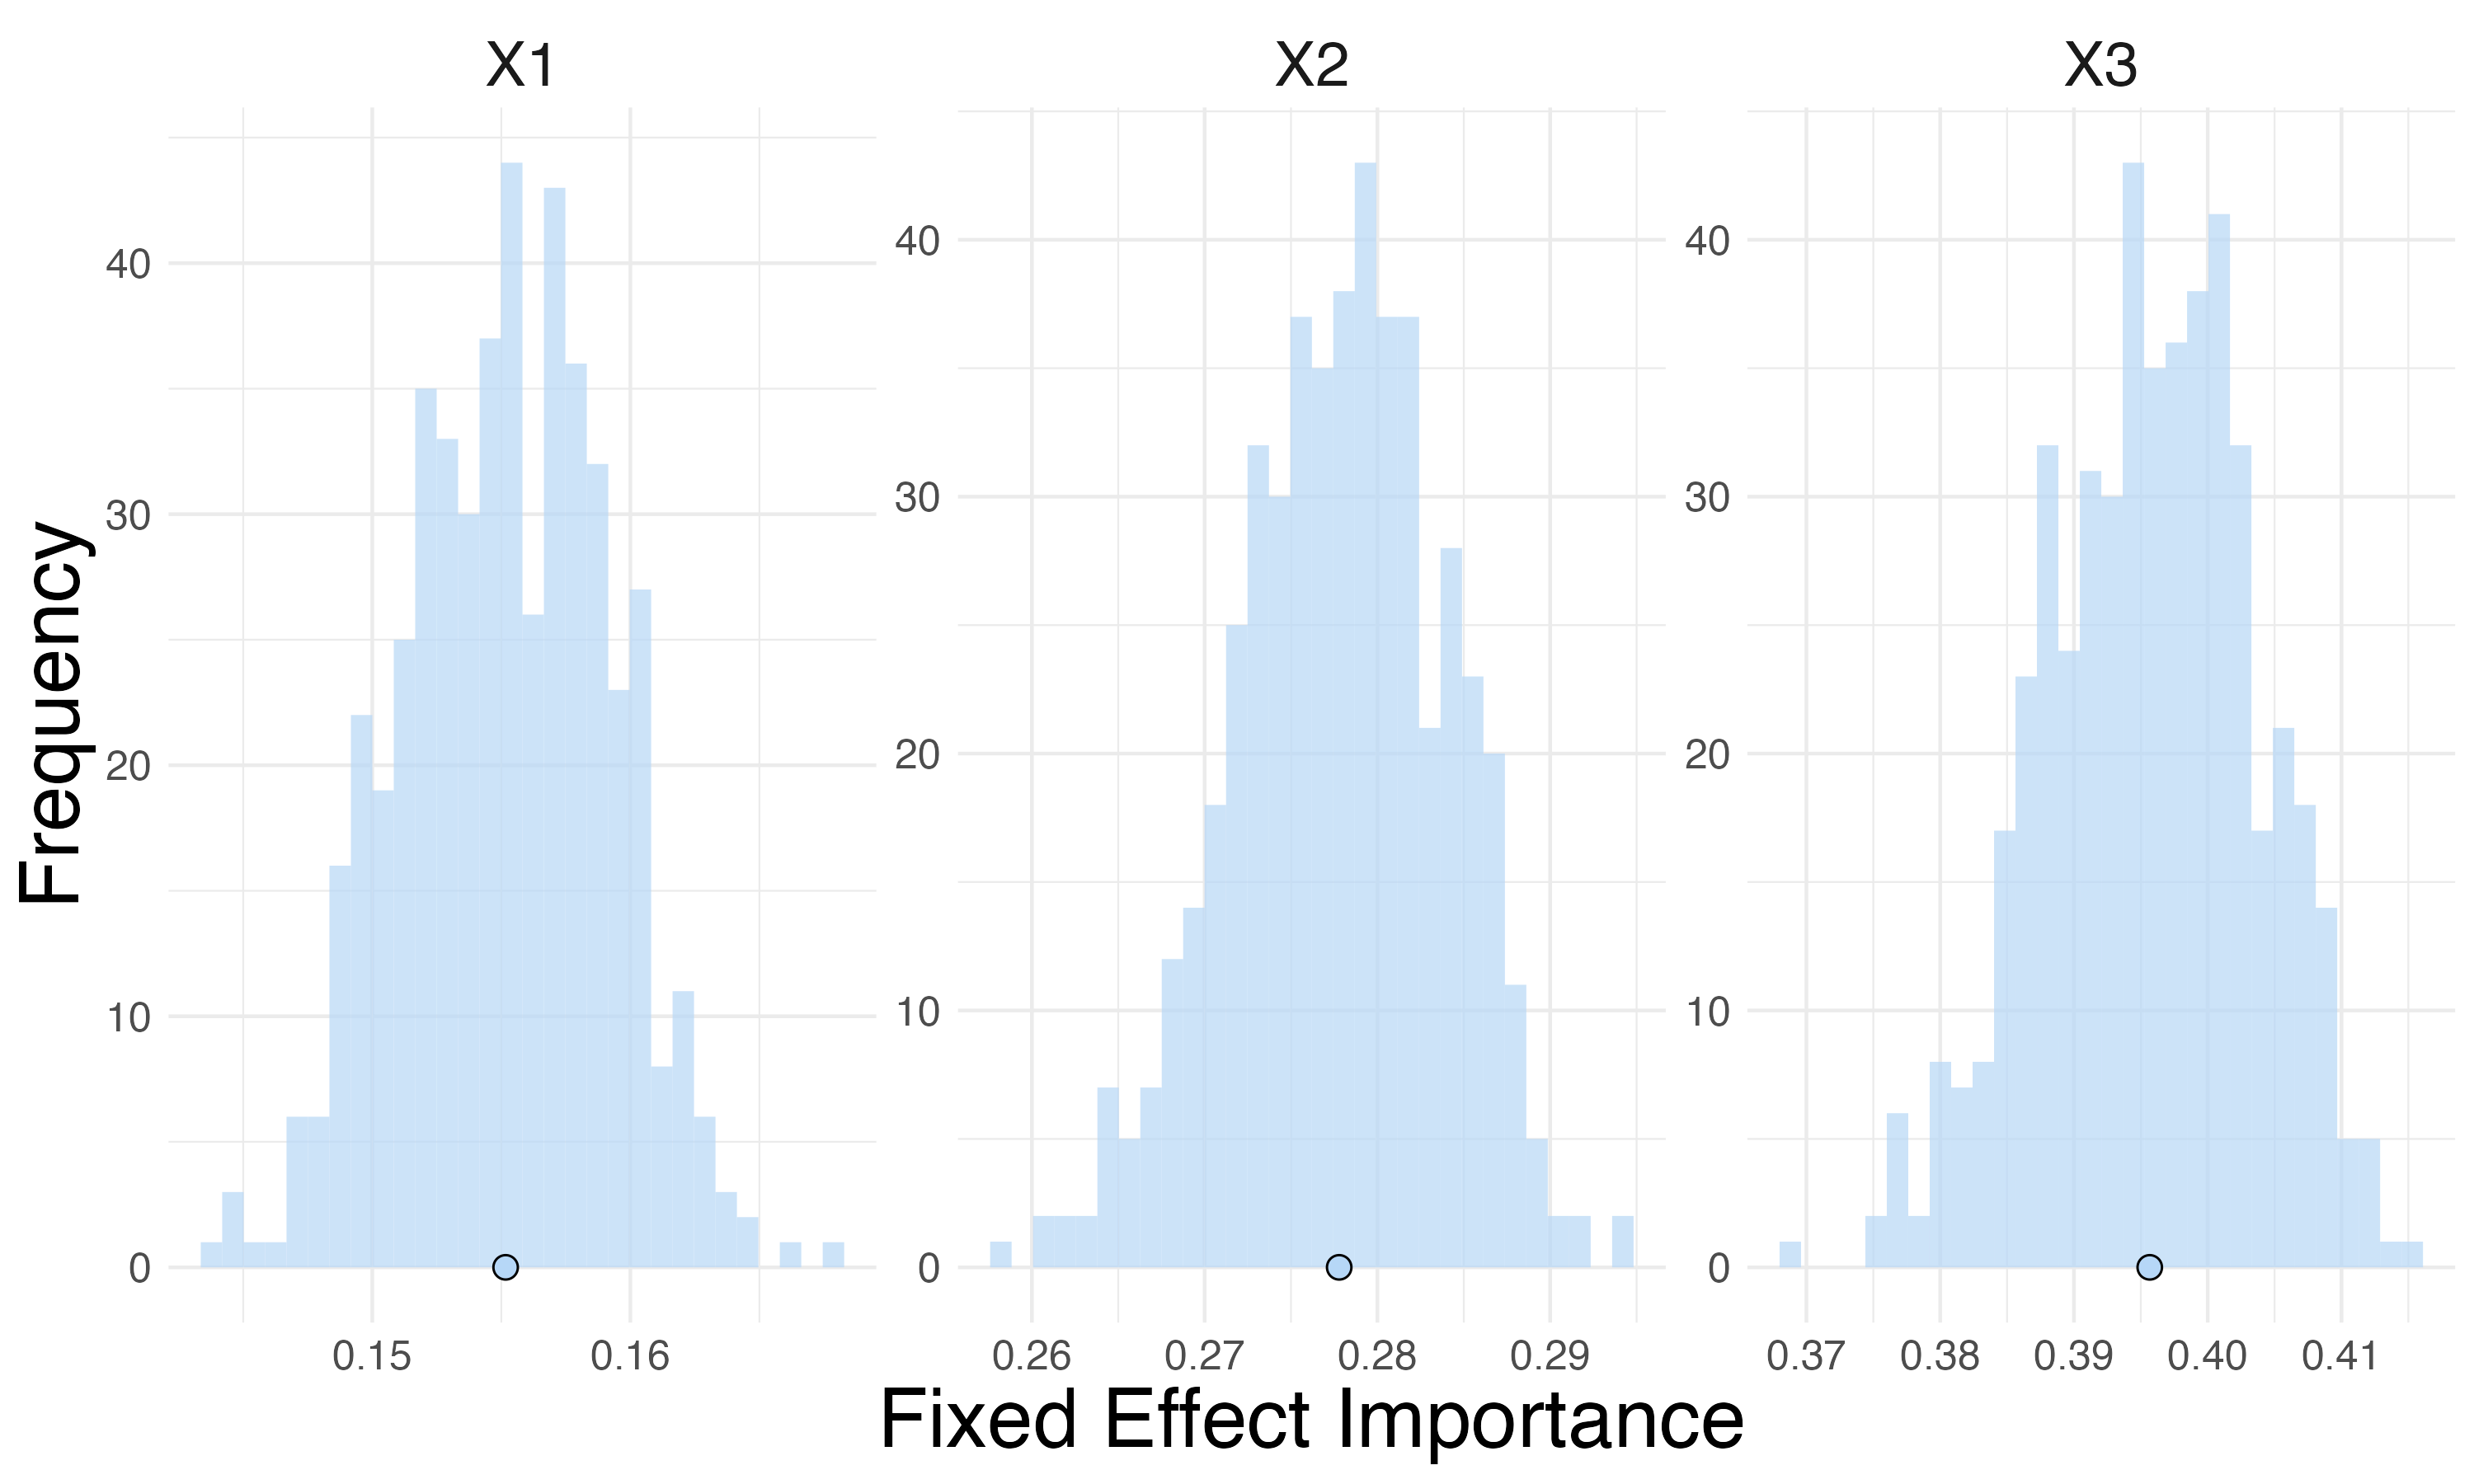
\includegraphics[width=1\linewidth]{Figures/Simulation study/Fixed_low_pos_poisson.png}
%   \caption{(d) Relative importance of the fixed effects $\mathbf{X_1},  \mathbf{X}_2, \mathbf{X}_3$ for $\rho=0.1$.}
%   \label{fig:fixed_effects_poisson_low_pos}
% \end{figure}
% \begin{figure}[H]\ContinuedFloat
%   \centering
%   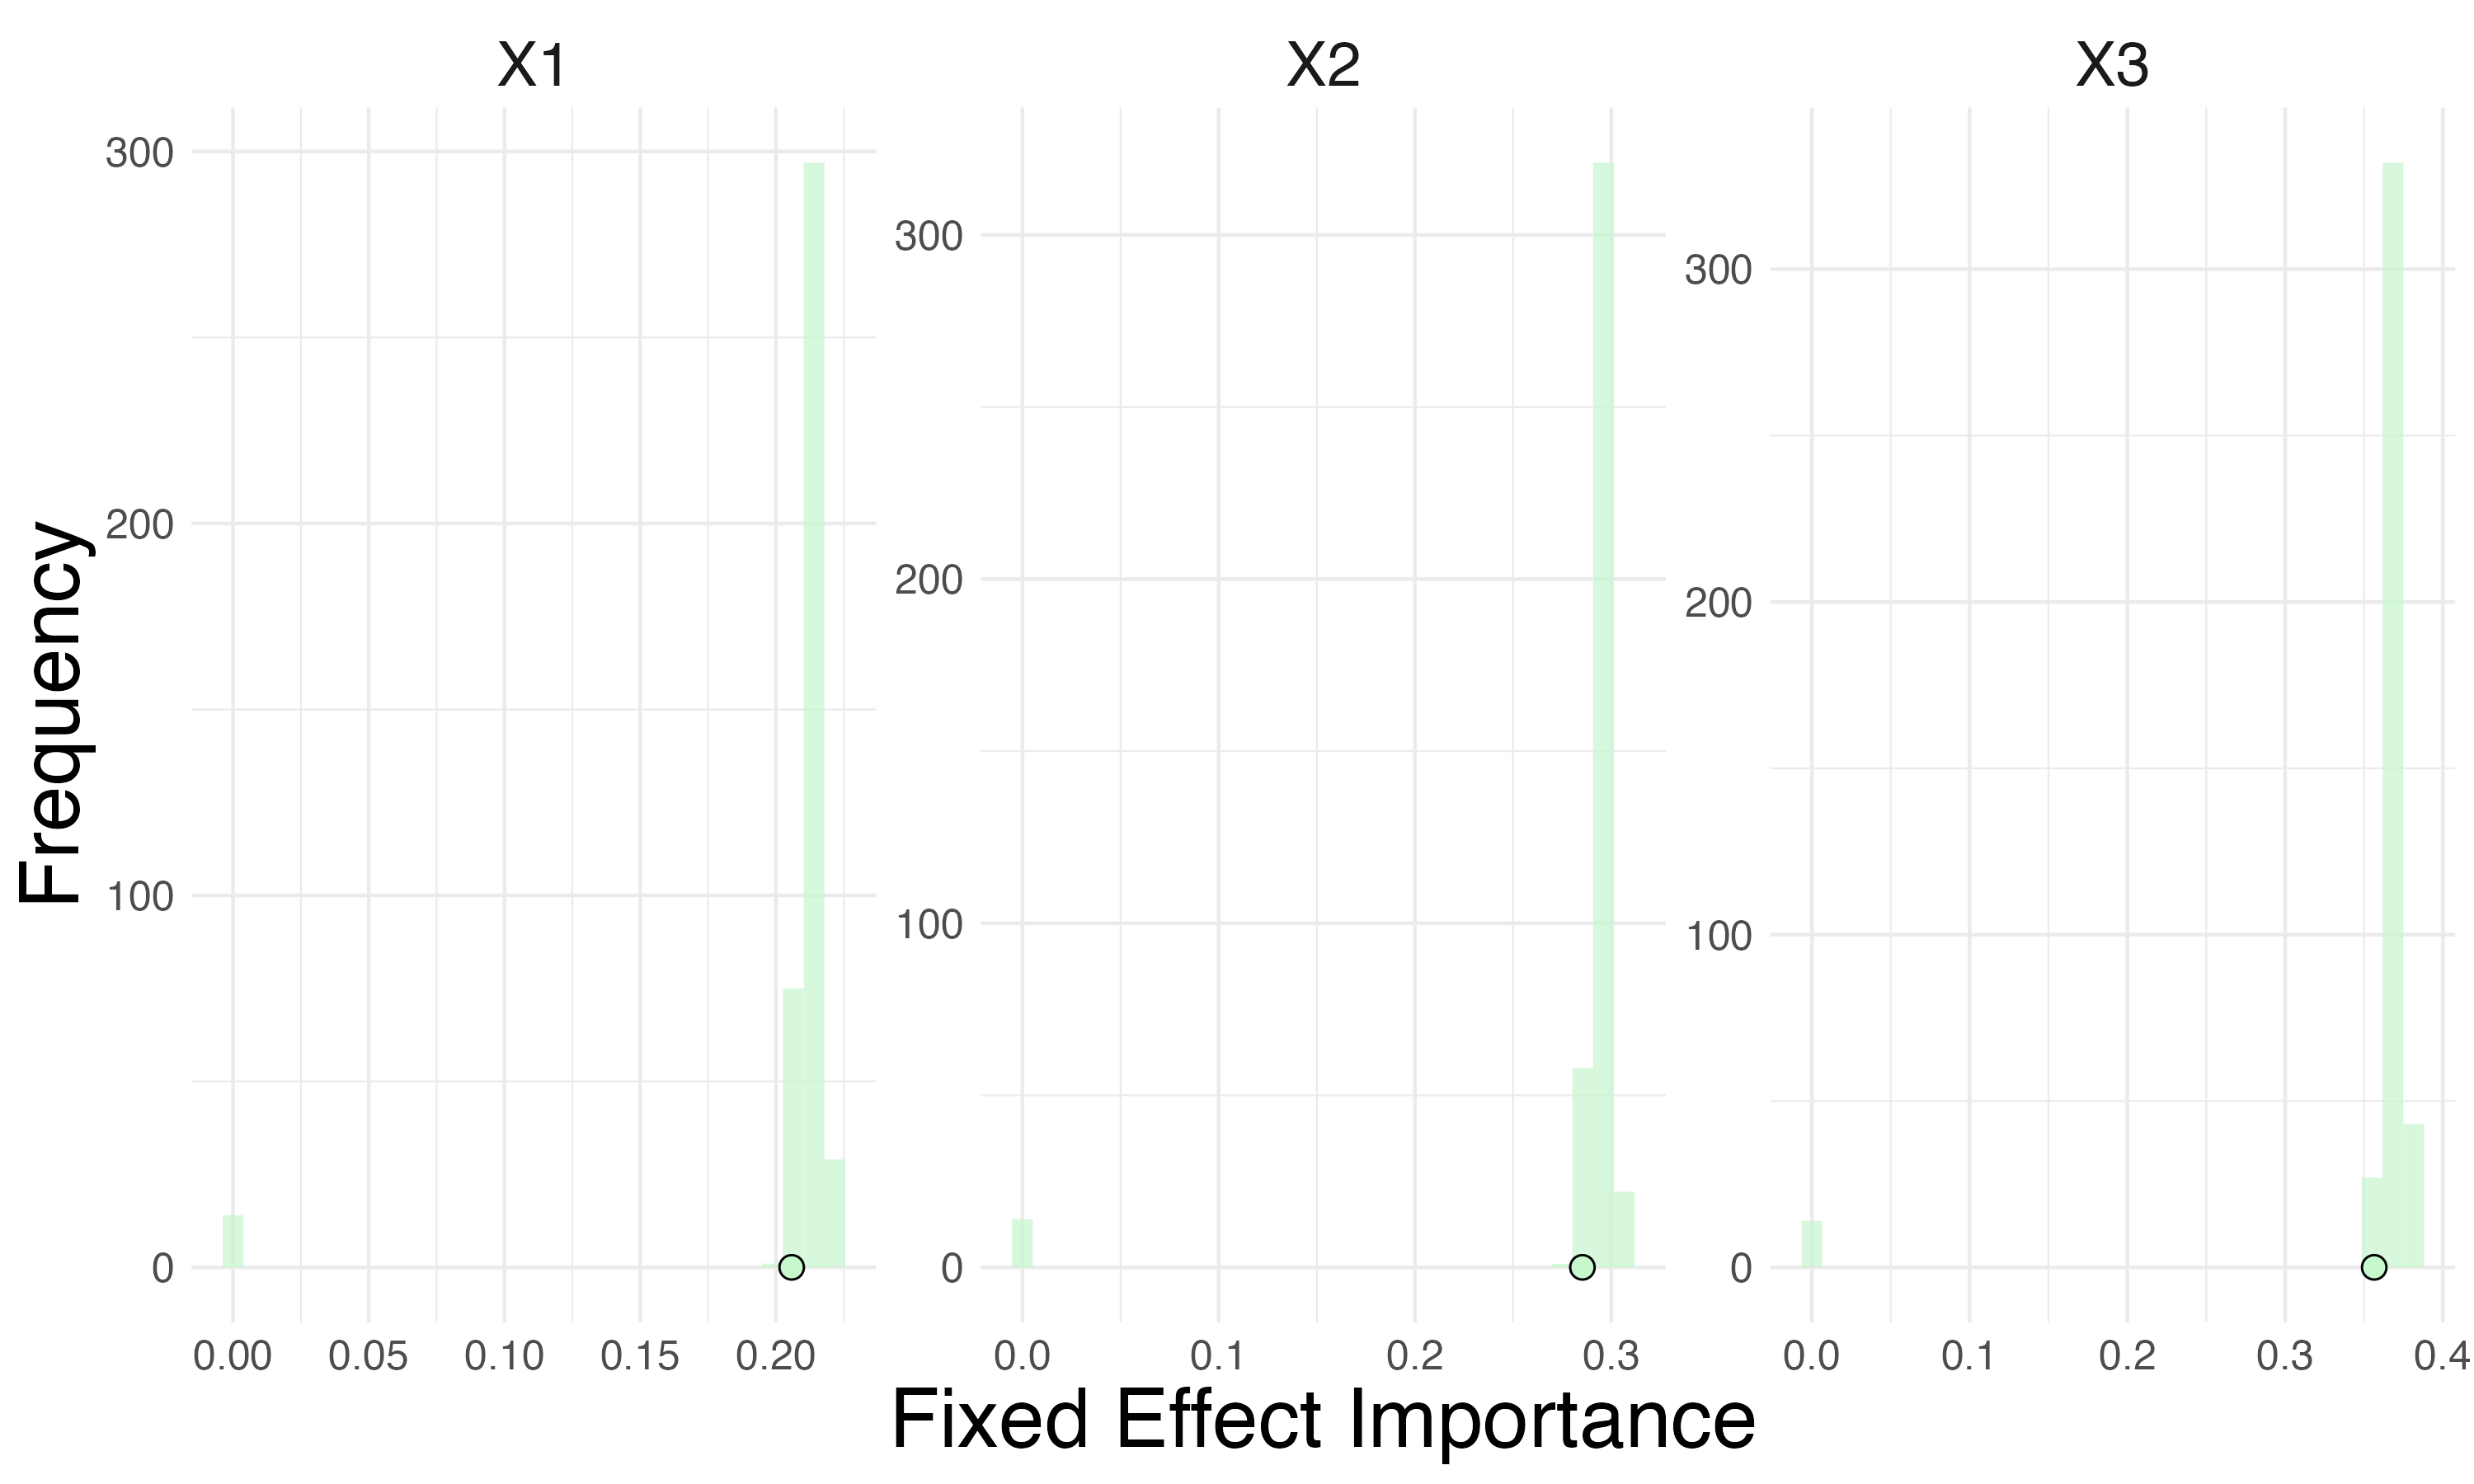
\includegraphics[width=1\linewidth]{Figures/Simulation study/Fixed_high_pos_poisson.png}
%   \caption{(e) Relative importance of the fixed effects $\mathbf{X_1},  \mathbf{X}_2, \mathbf{X}_3$ for $\rho=0.4$.}
%   \label{fig:fixed_effects_poisson_high_pos}
% \end{figure}
% \begin{figure}[H]
%   \centering
%   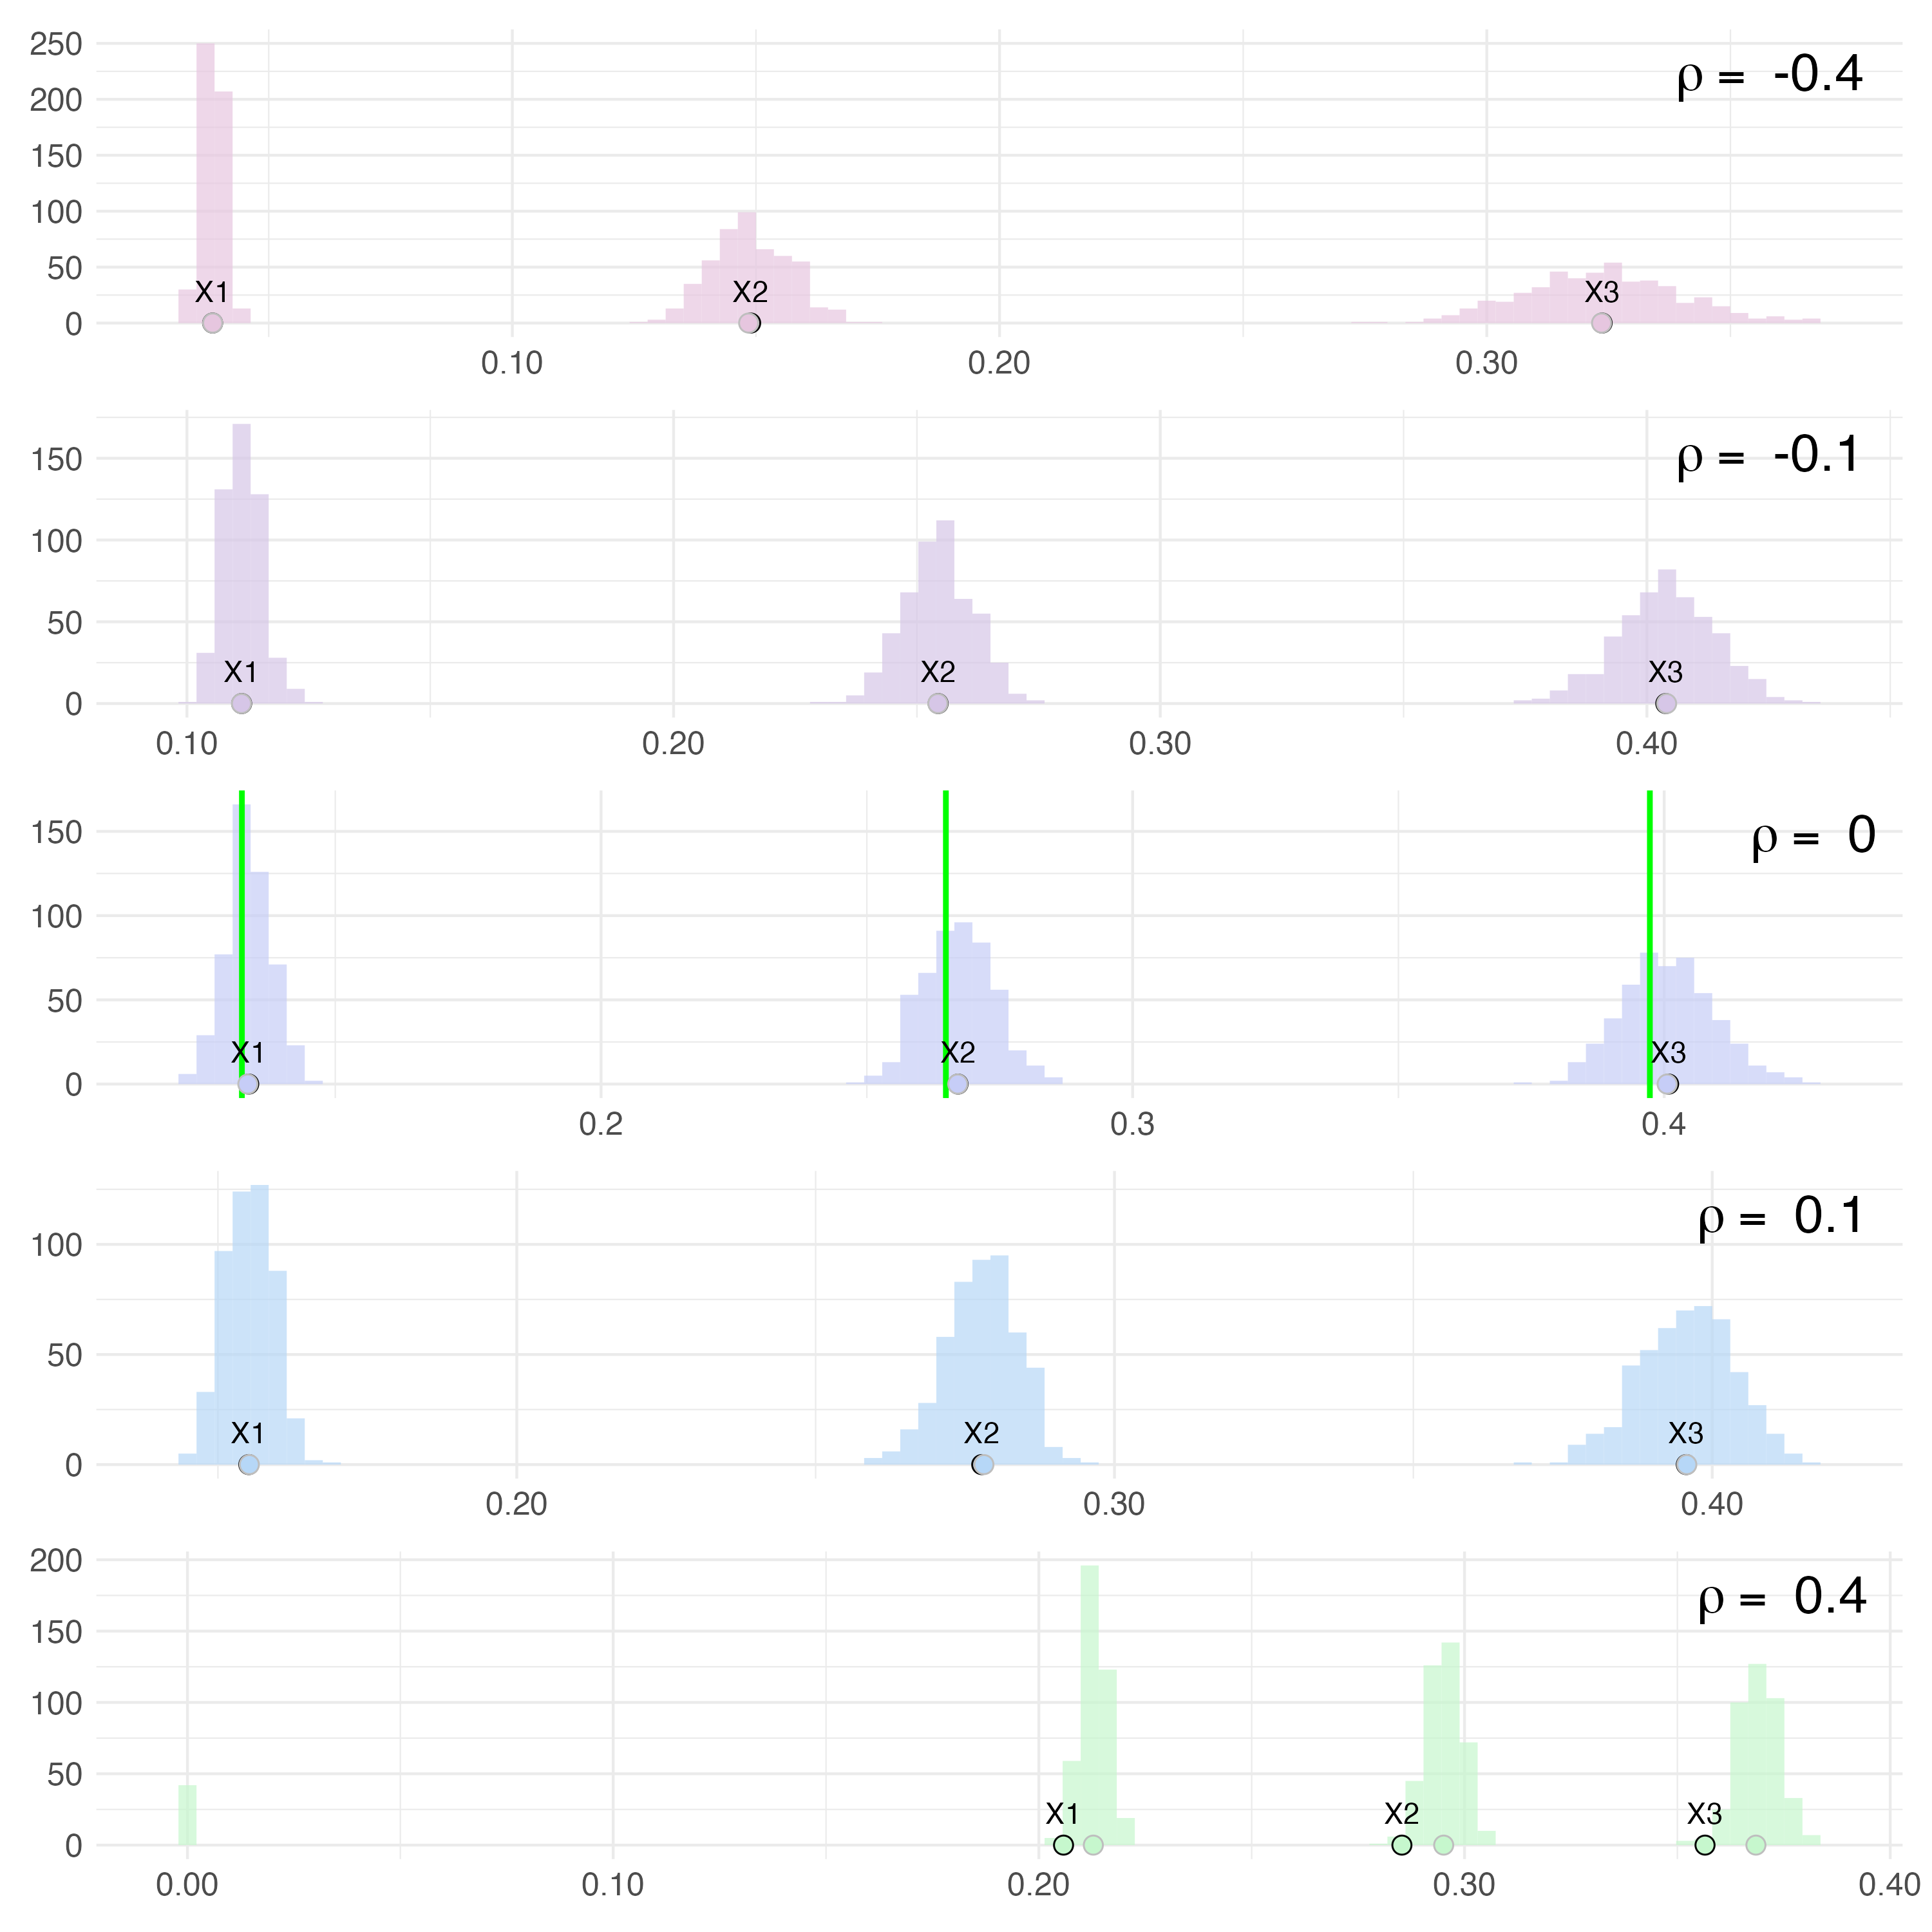
\includegraphics[width=1\linewidth]{Figures/Simulation study/Fixed_combined_poisson.png}
%   \caption{(e) Relative importance of the fixed effects $\mathbf{X_1},  \mathbf{X}_2, \mathbf{X}_3$ for $\rho=0.4$.}
%   \label{fig:fixed_combined_poisson}
% \end{figure}
\begin{figure}[H]
  \centering
  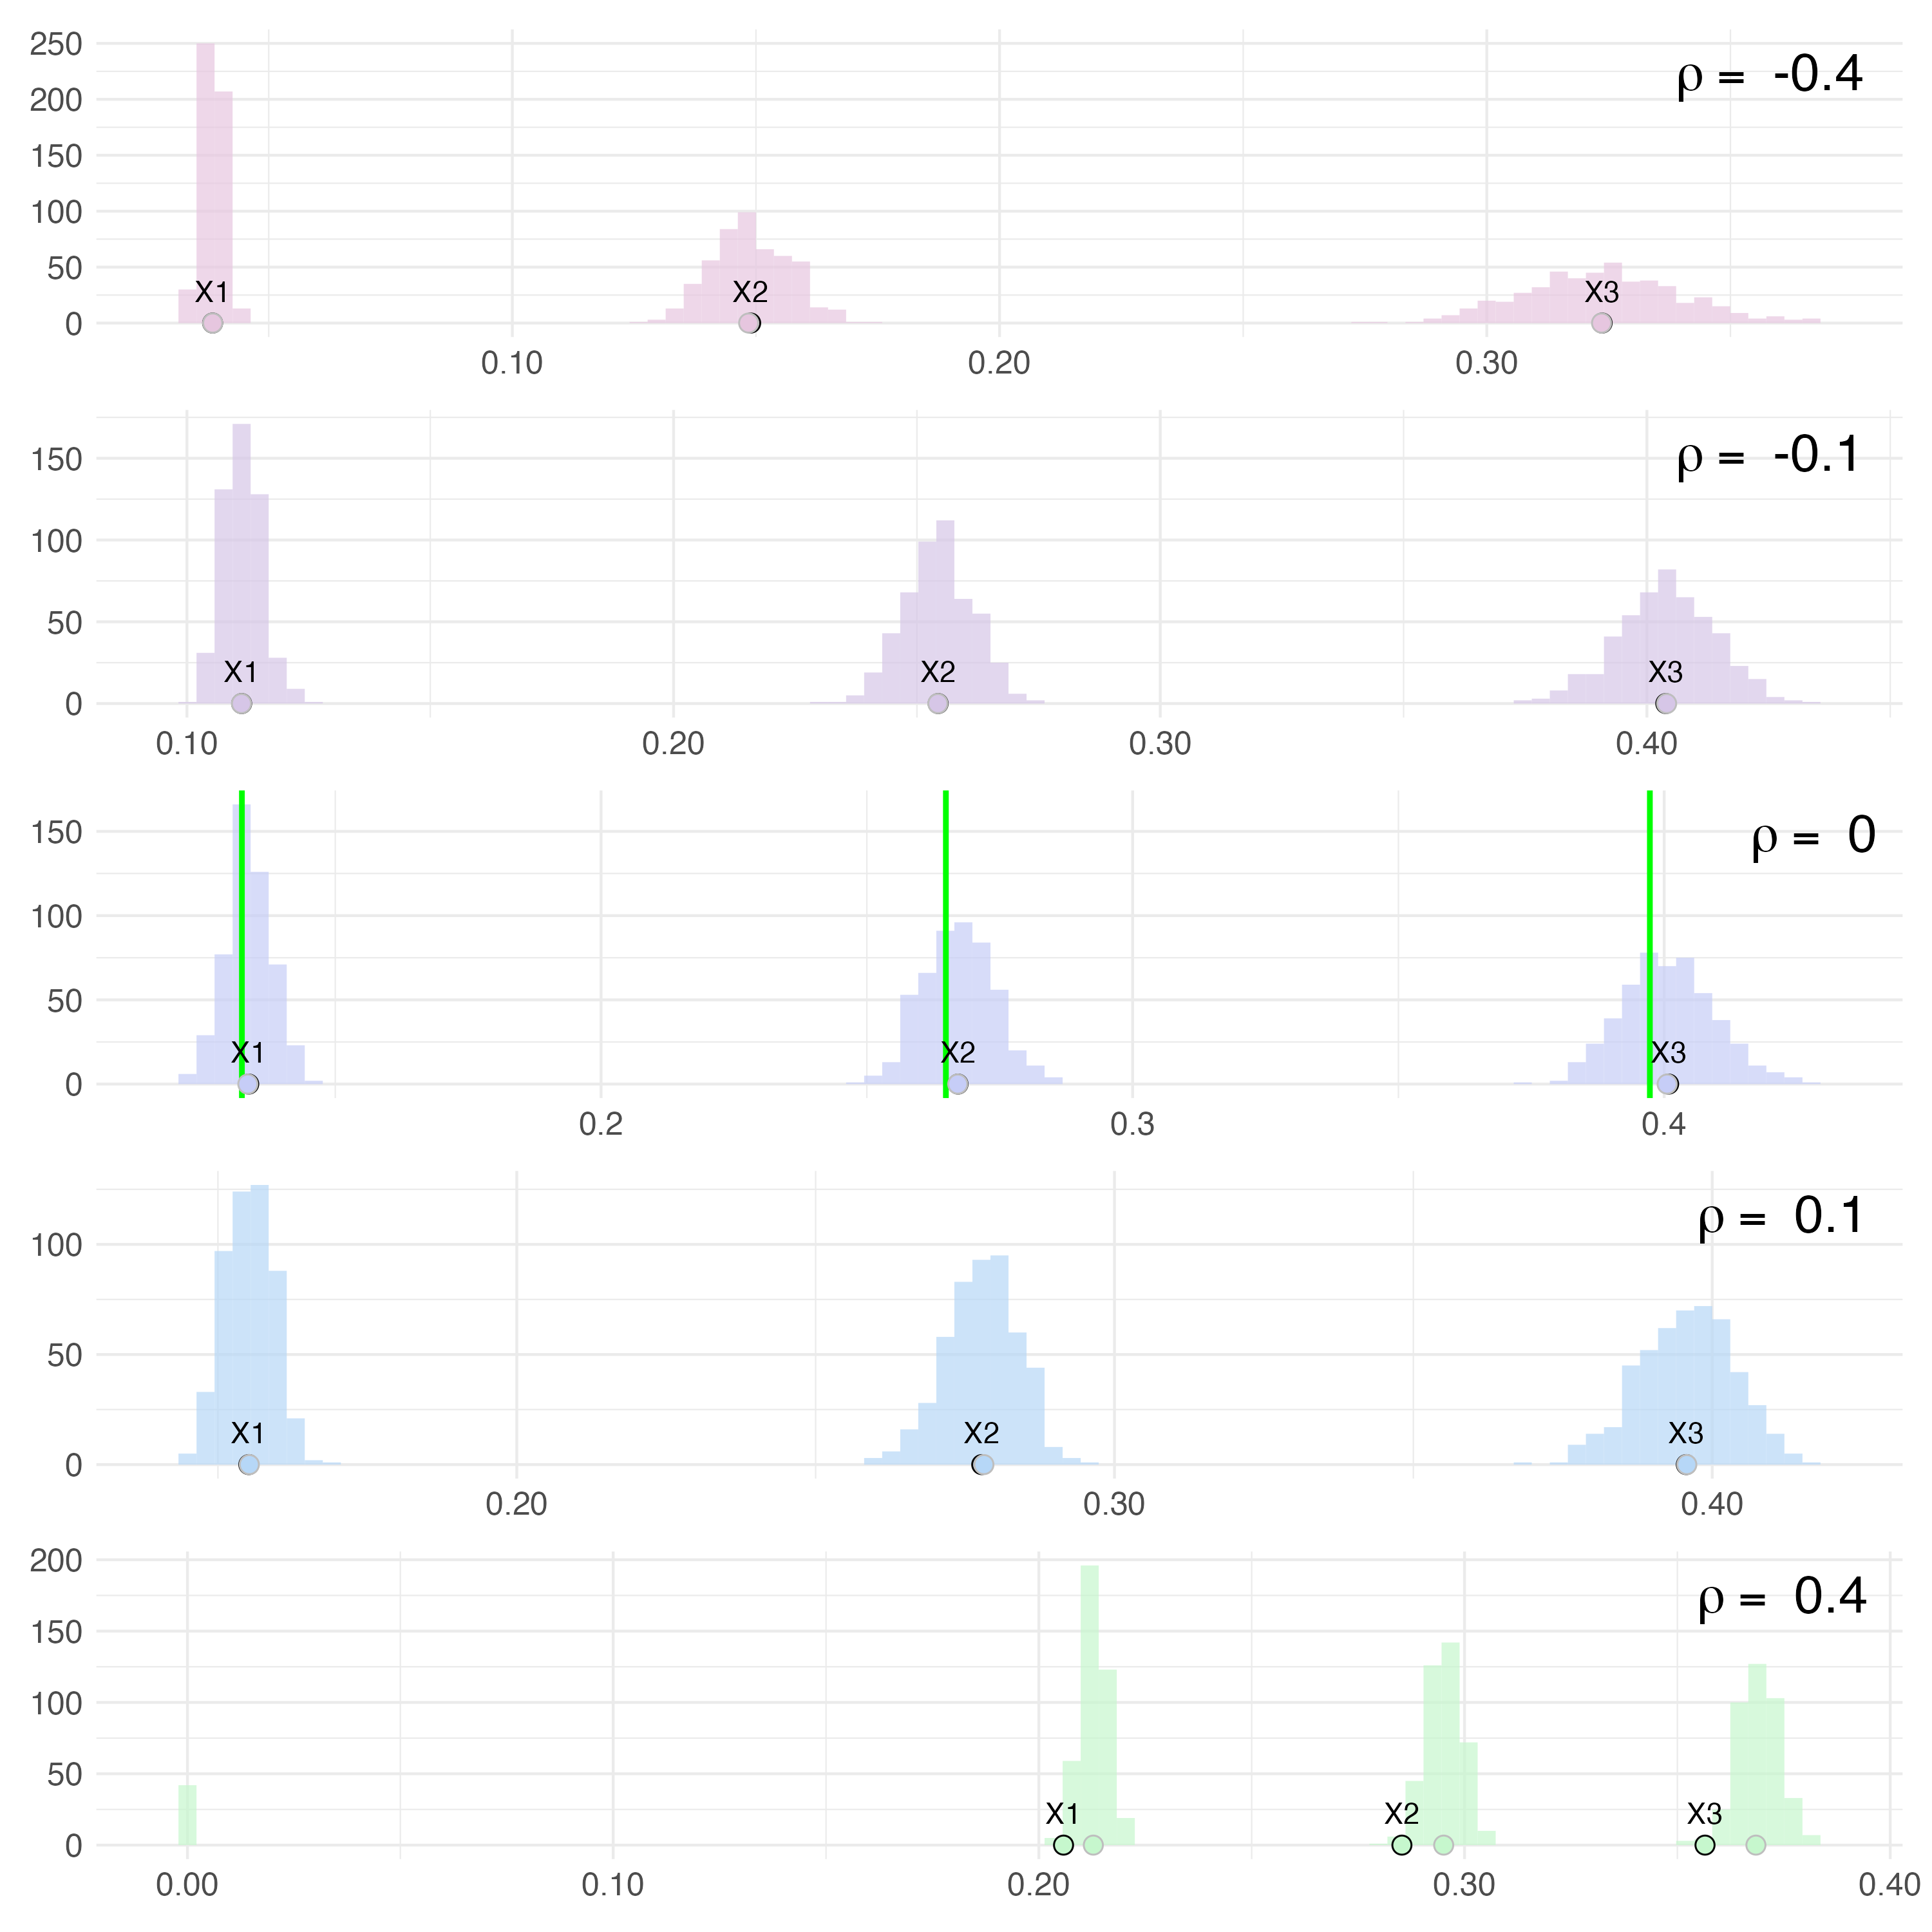
\includegraphics[width=1.1\linewidth]{Figures/Simulation study/Fixed_combined_poisson.png}
  \caption[Relative importance of the fixed effects in Poisson GLMM]{Histogram with the posterior modes of relative importance of the fixed effects present in the Poisson regression for the different correlation levels $\rho$. The modes are calculated by the Bayesian Variable Importance method from the $N_{\text{sim}}=500$ simulations in the simulation study. The true regression coefficients are $\boldsymbol{\beta}=(1, \sqrt{2}, \sqrt{3})^T$ and the vertical green line for $\rho=0$ displays the expected relative importance in the case of uncorrelated data. The mean of the modes for all simulations is denoted at the bottom of each histogram as a circle.}
  \label{fig:fixed_combined_poisson}
\end{figure}
\subsubsection{Random effect}
When looking at the sampled posterior distribution of relative importance estimates of the random effect in the Poisson model, we see that they too are in general a bit smaller than the same estimates for the binomial case (\Cref{fig:relimp_random_poisson}). This is again a consequence of the Poisson model having a relatively larger distributional variance, and so we expect these results. Likewise, the distributions can be said to be normal and symmetric around the mean also for the random effect in the Poisson model. We notice a somewhat larger spread in the random effect importances than the fixed effects for the Poisson model. The shrinkage effect of increasing correlation is also here apparent, with the average relative importance of the random effect going from $0.149$ for $\rho=-0.4$ to $0.072$ for $\rho=0.4$. We again emphasize that this is natural and anticipated, as the random effect variance is constant across correlation levels, while the variance of the fixed effects vary. The expected value when $\rho=0$ is $0.097$ as shown in \Cref{table:3}, and we see that the average estimate is close to this value. The orange dots, denoting the estimates from the \texttt{rptR} package are close to the average estimate from the BVI method, with the largest difference being seen for $\rho=0.4$ with a difference of $0.017$. This is also the largest relative difference, being $24\%$ of the average estimated relative importance. The method seems to be in agreement with the expected values for the relative importance of the random effect, and the \texttt{rptR} estimates are close to the BVI method.
% \\
% \\
% As previously mentioned, for $\rho=0.4$, some models estimated all the fixed effects to be zero. As a consequence of this, the random effect for these models are in turn estimated to have a corresponding larger importance,  due to the way we have defined relative importance. Although it is not so clear from \Cref{fig:relimp_random_poisson}, it can be seen that we have values of approximately $0.3$, $0.9$ and $1$ when $\rho=0.4$. Again, albeit unfortunate, we believe that the method correctly estimates the relative importance, based on the given model, and that the fitted models might be results of some problem with the simulated data or INLA.
\begin{figure}[H]
  \centering
    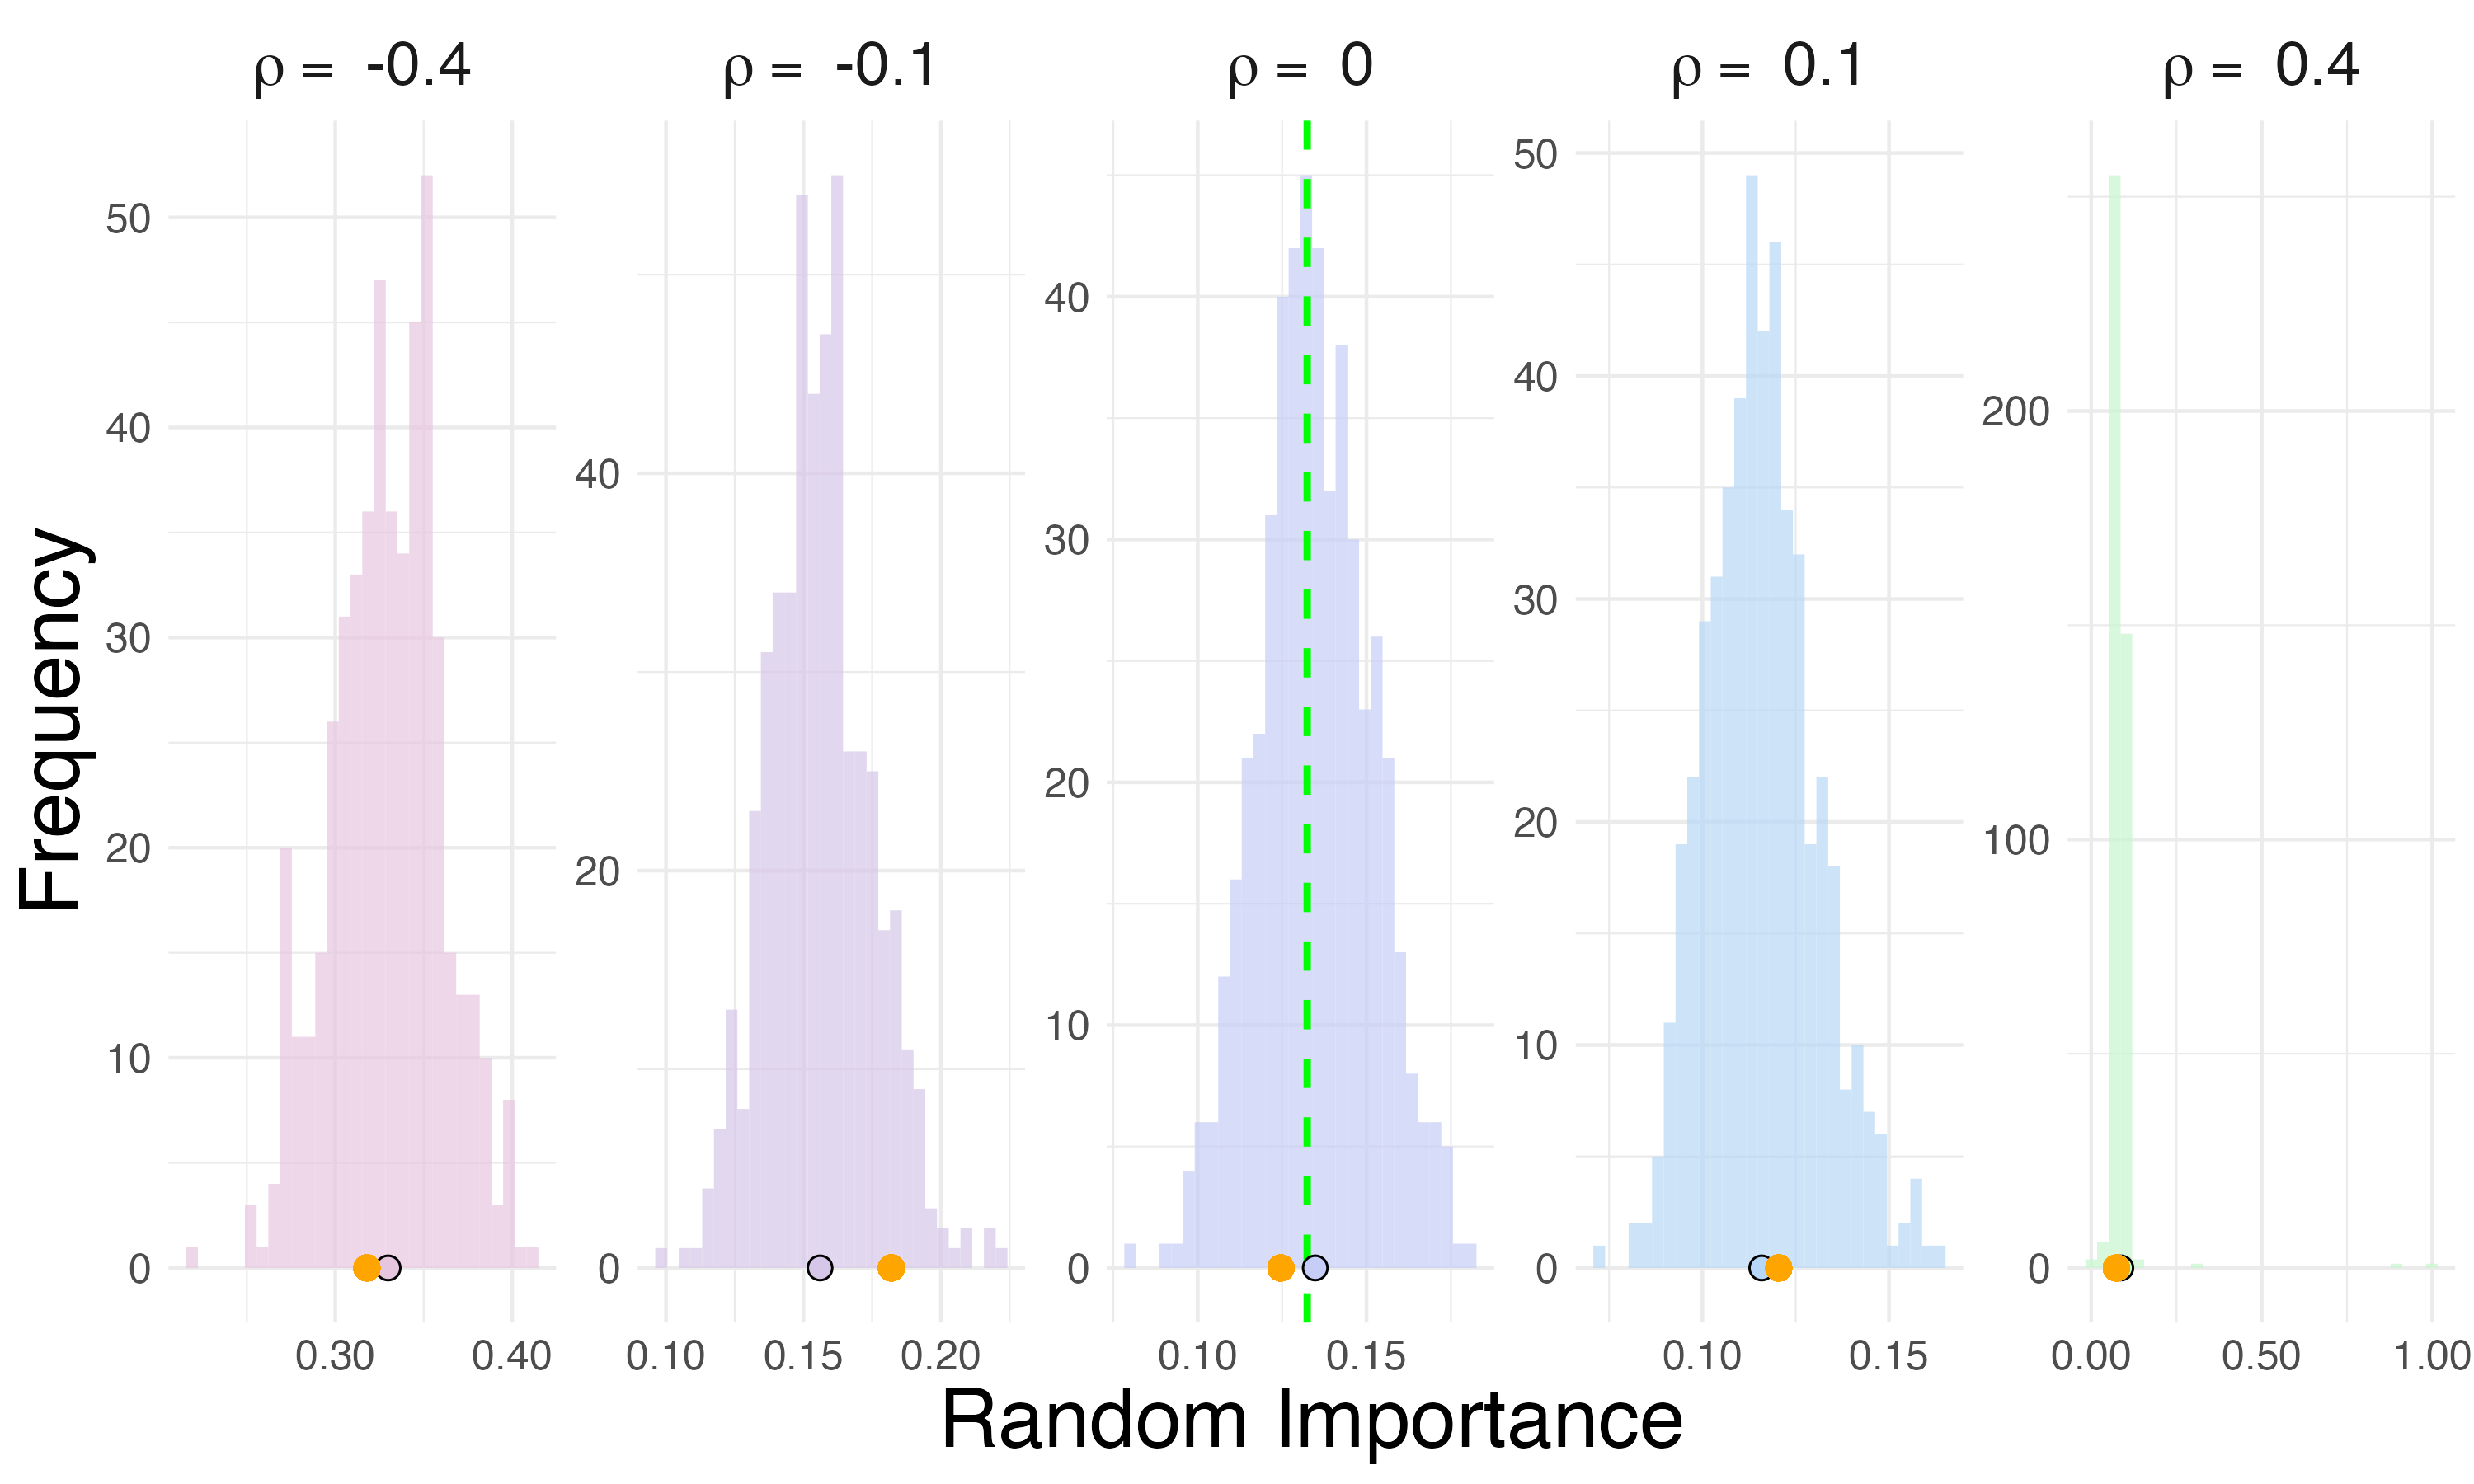
\includegraphics[width=1\linewidth]{Figures/Simulation study/Random_poisson.png}
    \caption[Relative importance of the random effect $\boldsymbol{\alpha}$ in Poisson GLMM]{Histogram with posterior modes of the relative importance estimates for the random effect $\boldsymbol{\alpha}$ for varying values of $\rho$ calculated by the BVI method. The study conducted $N_{\text{sim}}=500$ simulations and the mean of the mode of relative importance for all simulations is displayed at the bottom of each histogram as a circle. The vertical green line for $\rho=0$ is the expected relative importance as in \Cref{table:3} and the orange dot is the corresponding estimate from the \texttt{rptR} package.}
    \label{fig:relimp_random_poisson}
\end{figure}
\subsubsection{$R^2$ estimates}
Moving on to the estimated posterior $R^2$ distributions for the Poisson model (\Cref{fig:r2_combined_poisson}), we see that the expected values from \Cref{table:r2values} are in close agreement with the average marginal and conditional $R^2$ estimated from the BVI method for all correlation levels. The largest difference in expected values and average values from the BVI method is found for $\rho=0$ and is $0.001$ for the marginal and for the conditional $R^2$ the difference is negligible. The $R^2$ distributions seem roughly normal and symmetric around the mean value, with a plausible size of the spread. Again, there are some more notable differences between the BVI method and the \texttt{rptR} package. For $\rho=0.1$ we observe the difference to be $0.010$ for the marginal $R^2$ and for the conditional $R^2$ when $\rho=-0.4$ it is also $0.010$. These differences are $2\%$ and $4\%$ of the average estimated values, respectively. In general, we also see here that our method aligns closely with our expectation, and deviates a bit more from the \texttt{rptR} package estimates.
% Contrary to what was the case, it now seems that the BVI method consistently estimates lower values than the \texttt{rptR} package. The estimates from the \texttt{rptR} package deviate quite a bit from our method, and they seem to deviate more as the correlation increases. For $\rho=-0.4$ the methods agree, but in general the differences are noticeable. It is hard to say why this occurs, especially since our method coincides very closely with the expected values as well.
% A possible explanation for this, is that the \texttt{rptR} package internally estimates an overdispersion parameter for Poisson models. This is then 
% and are consistently larger for both marginal and conditional $R^2$. Overall, the distributions seem to form a reasonably symmetric normal curve centered at the mean, close to what we would expect.
% \begin{figure}[H]
%   \centering
%   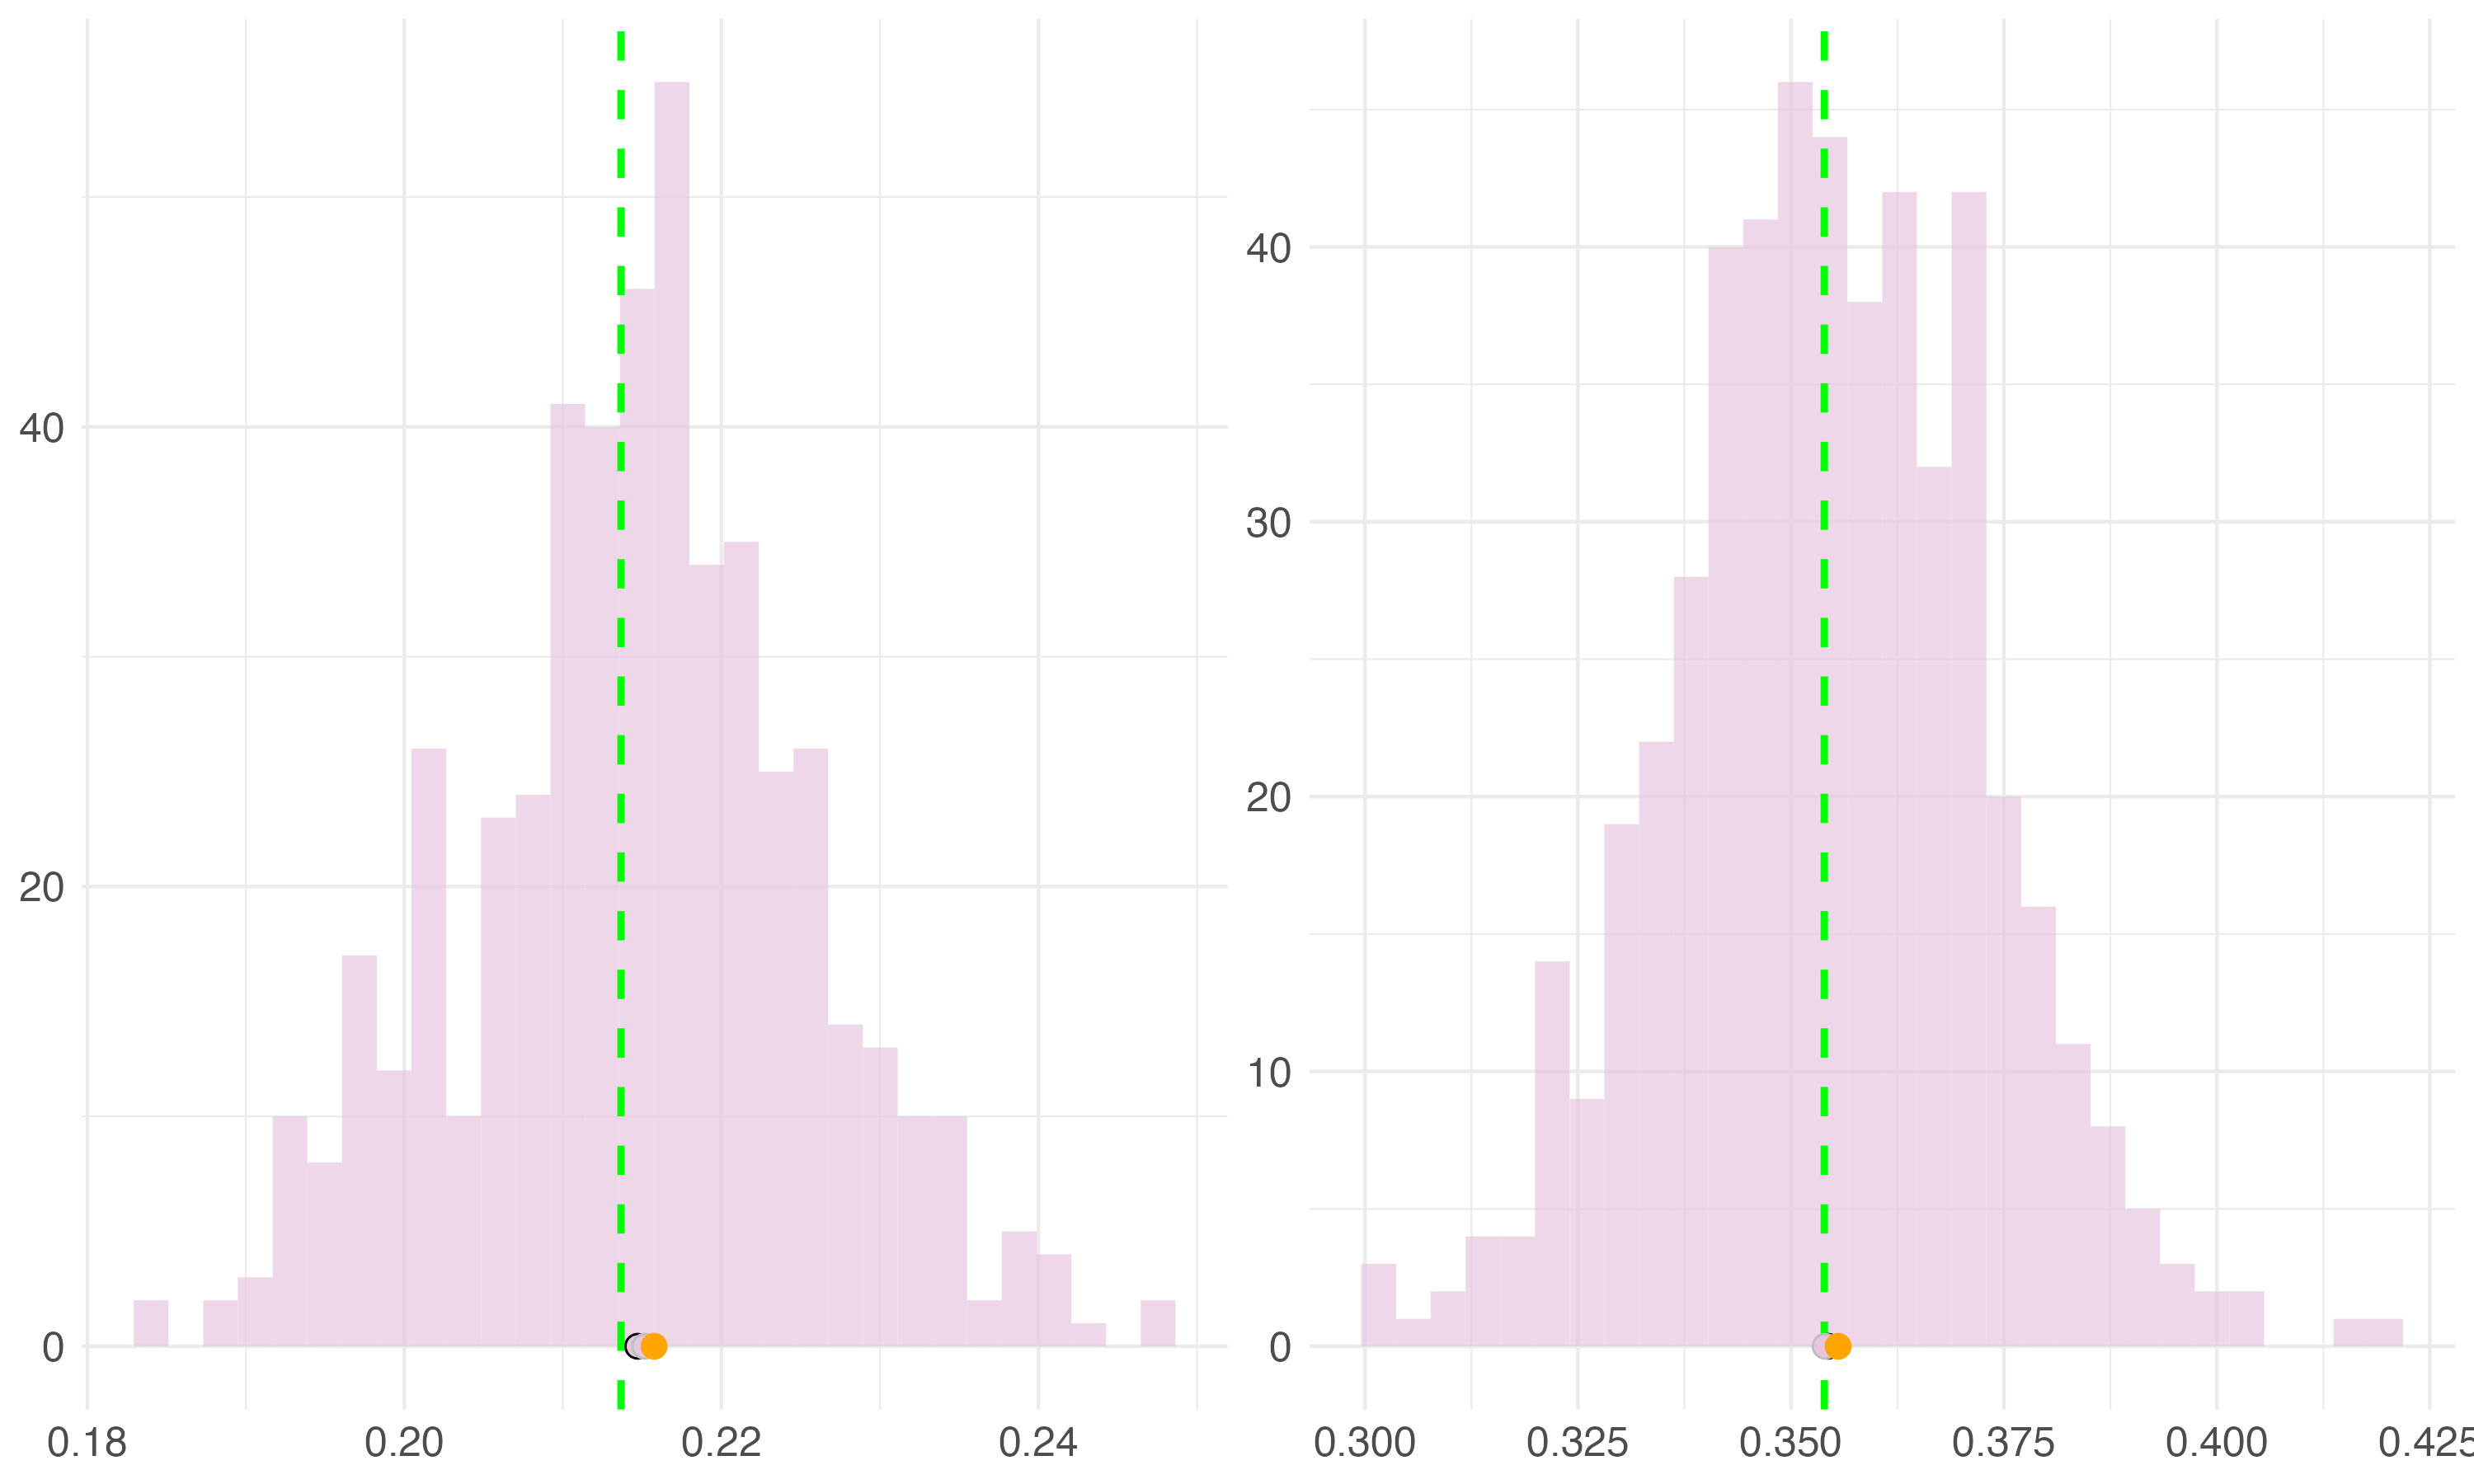
\includegraphics[width=1\linewidth]{Figures/Simulation study/R2_poisson_high_neg.png}
%   \caption{Histogram for the estimated marginal $R^2$ (left) and conditional $R^2$ (right) for the Poisson regression using the BVI method. The results are from the $N_{\text{sim}}=500$ simulations in the simulation study for different correlation levels $\rho$. The expected values are displayed as vertical green lines, and can be found in \Cref{table:r2values}. The mean value of the $R^2$ values for all simulations is marked with a circle at the bottom. (a) Marginal and conditional $R^2$ estimates for $\rho=-0.4$.}
%   \label{fig:r2_poisson_high_neg}
% \end{figure}
% \begin{figure}[H]\ContinuedFloat
%   \centering
%   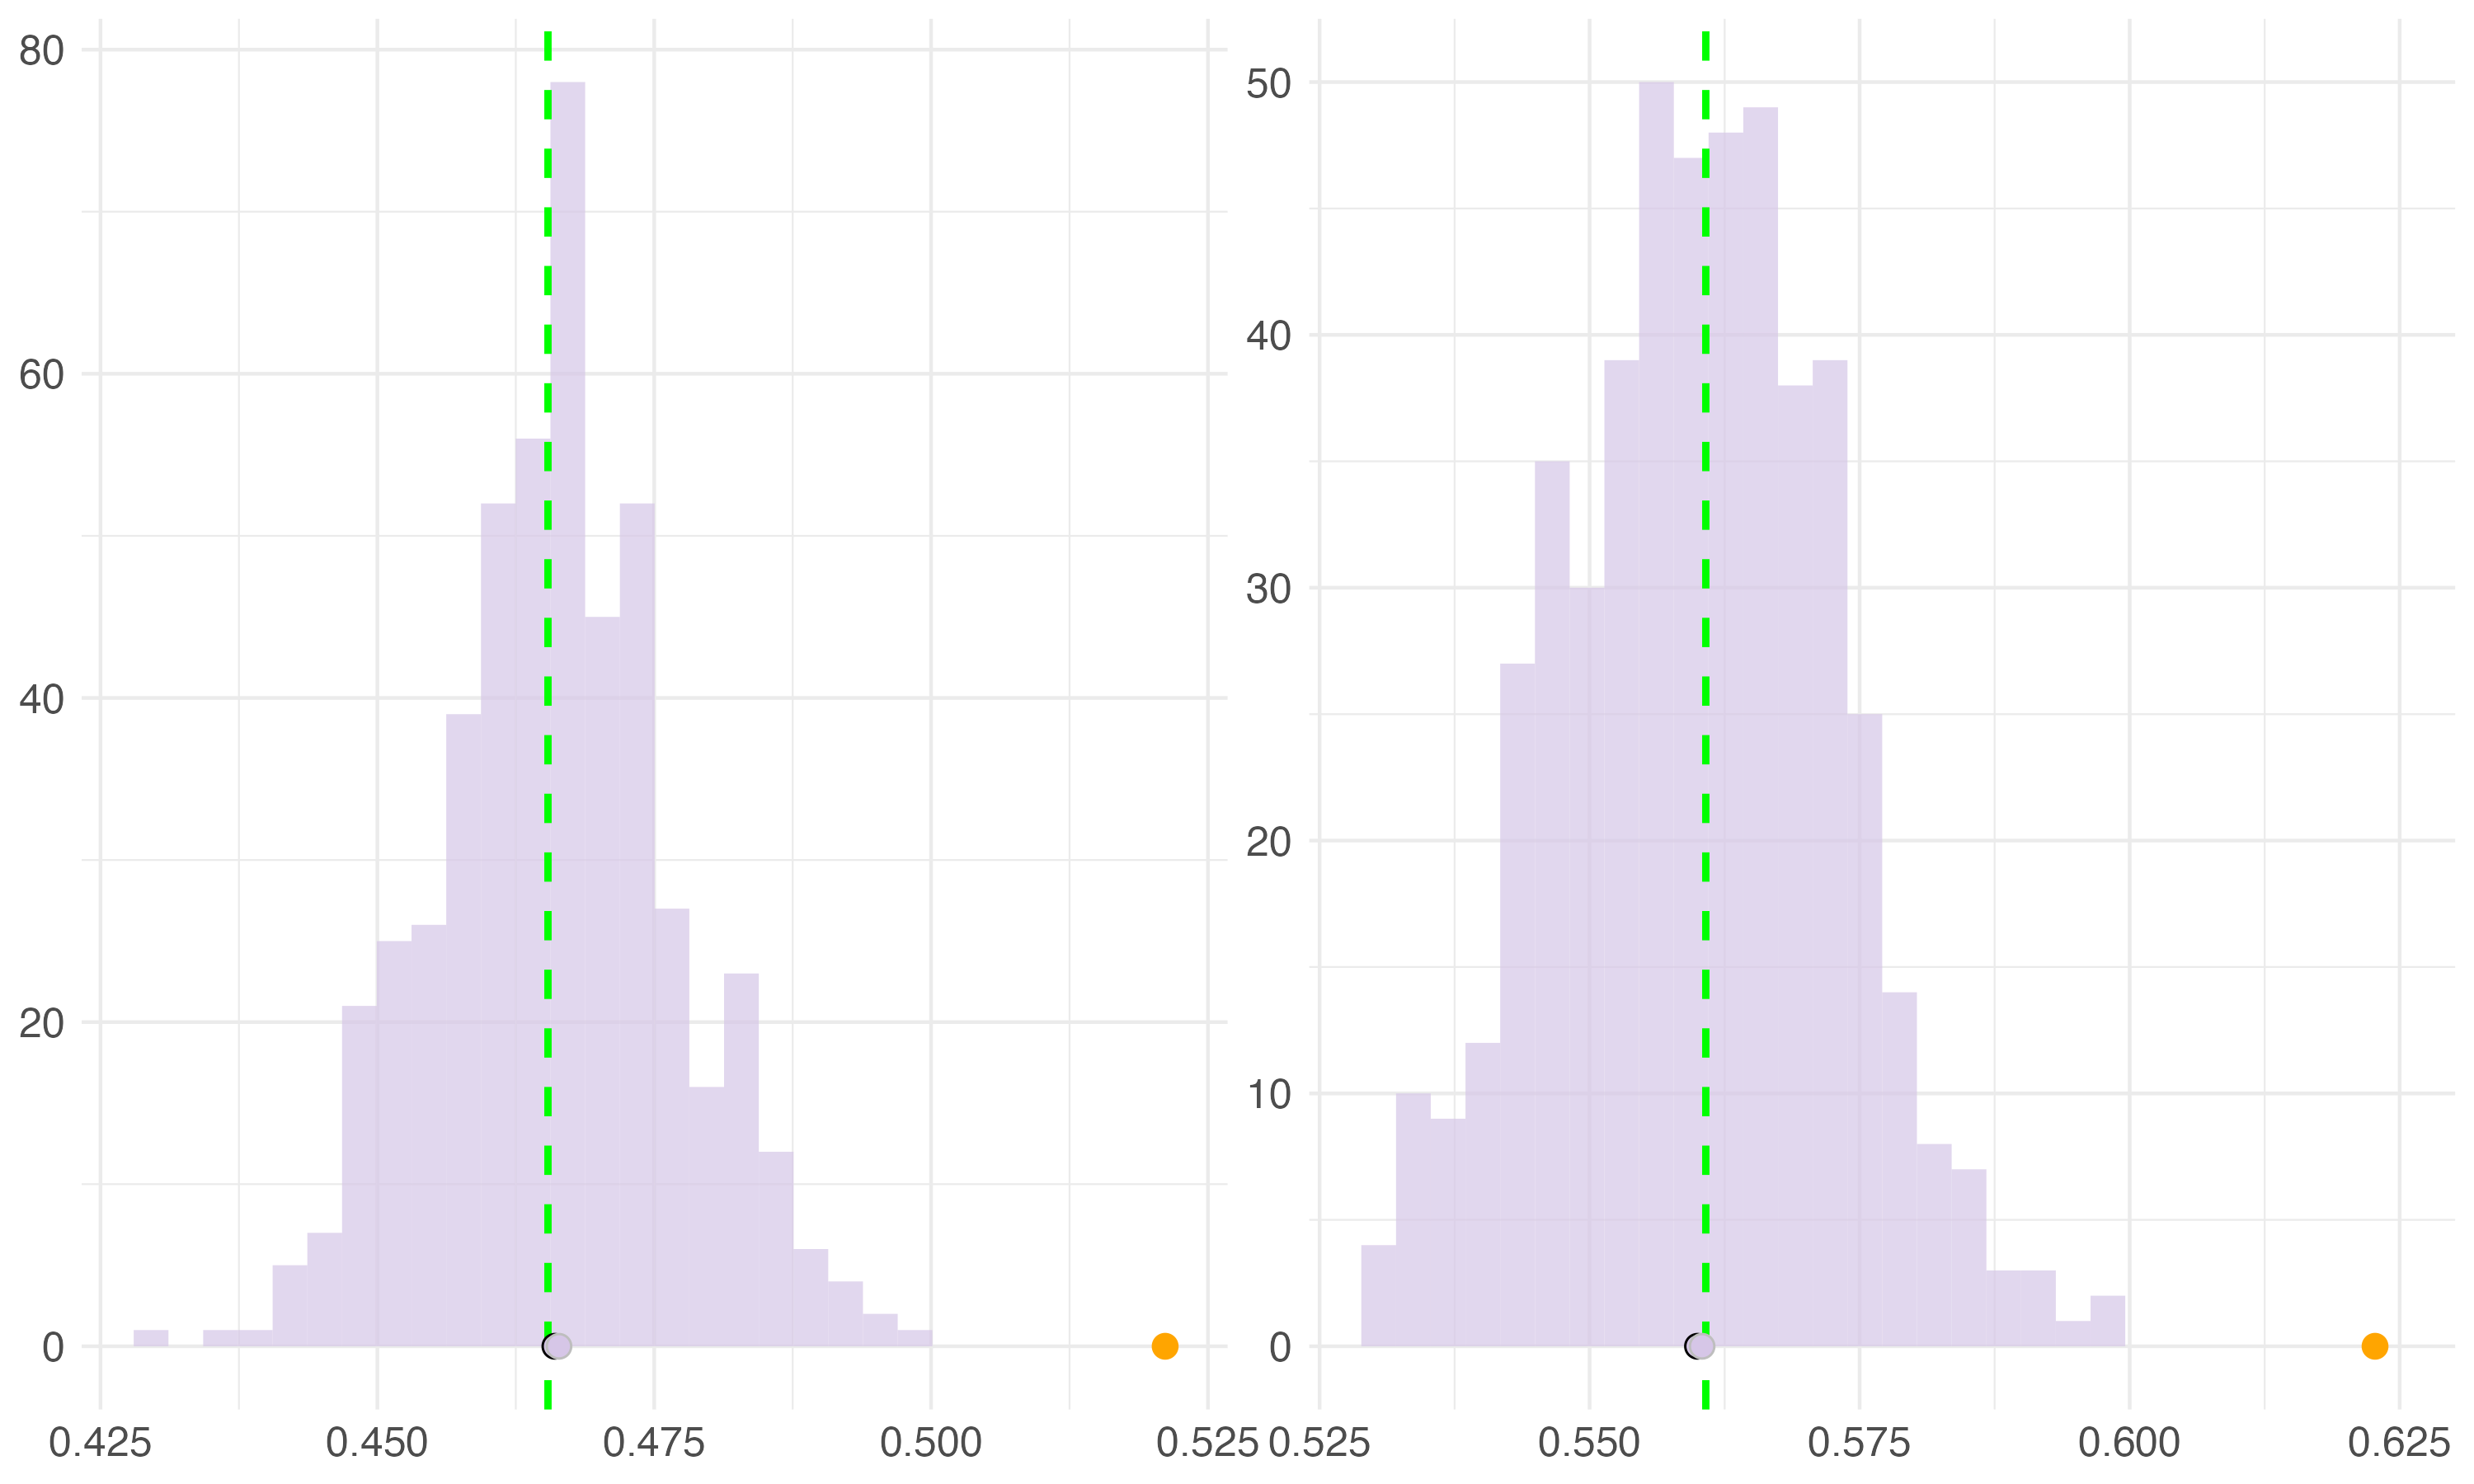
\includegraphics[width=1\linewidth]{Figures/Simulation study/R2_poisson_low_neg.png}
%   \caption{(b) Marginal and conditional $R^2$ estimates for $\rho=-0.1$.}
%   \label{fig:r2_poisson_low_neg}
% \end{figure}
% \begin{figure}[H]\ContinuedFloat
%   \centering
%   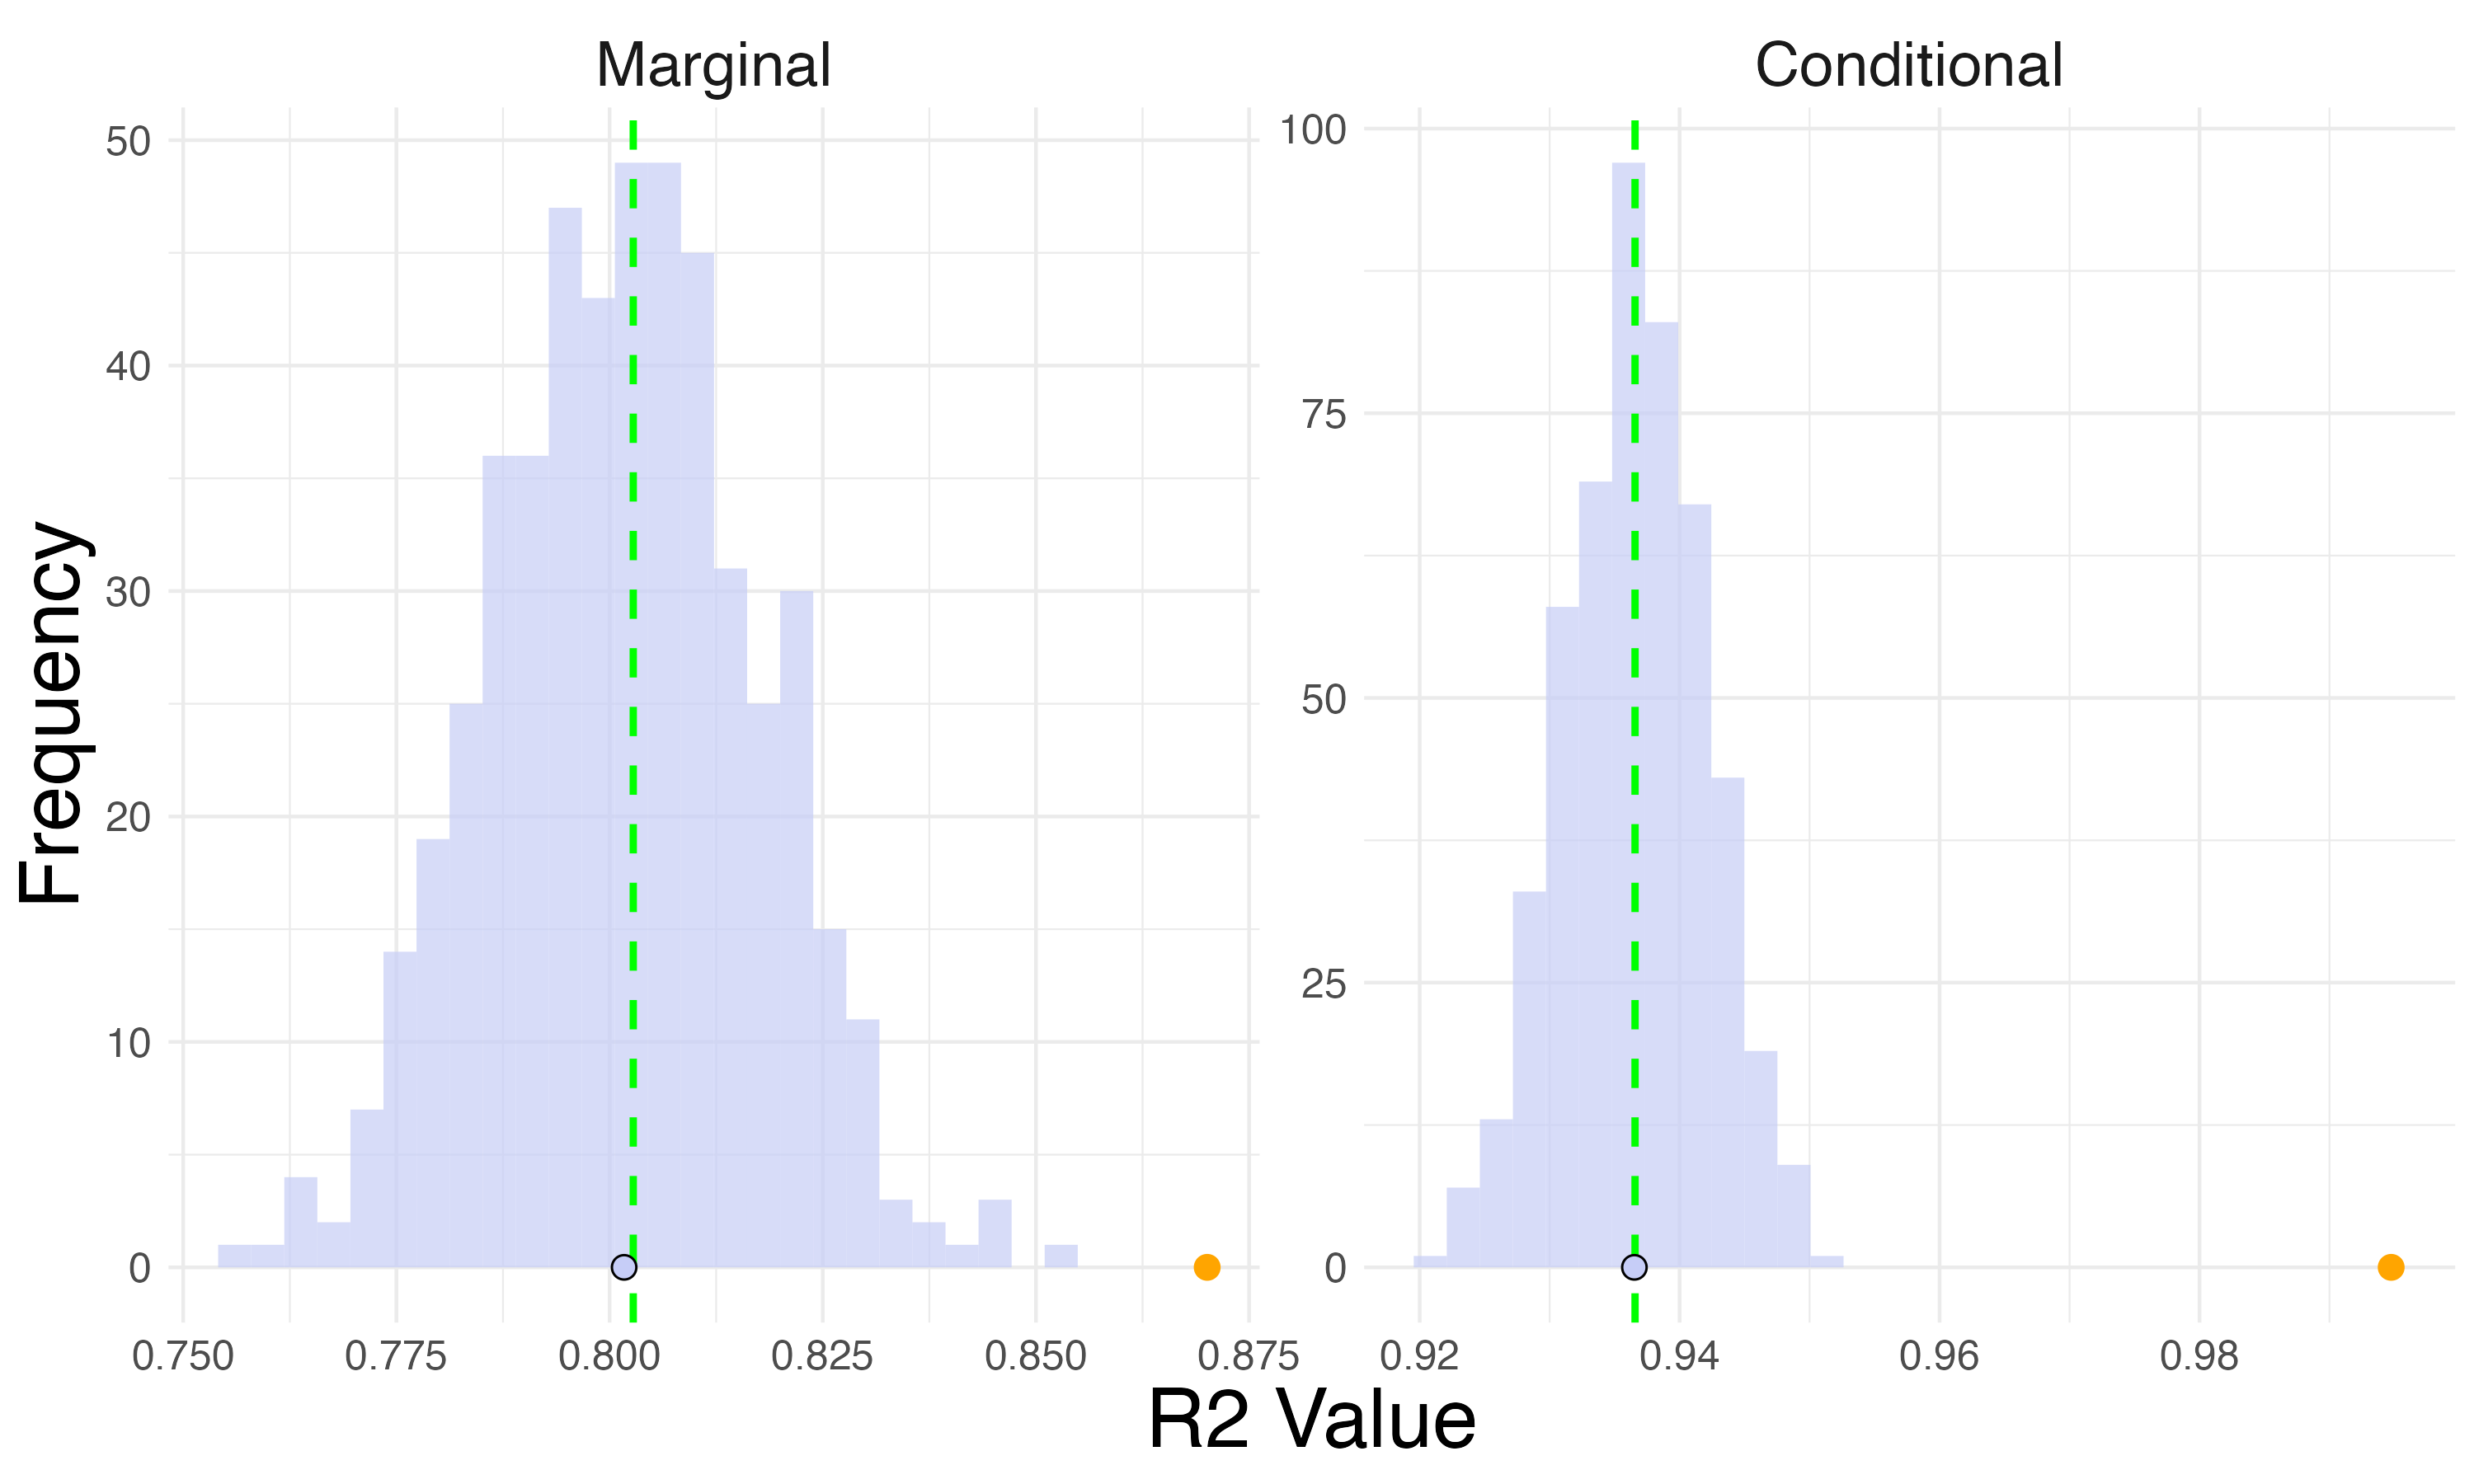
\includegraphics[width=1\linewidth]{Figures/Simulation study/R2_poisson_no.png}
%   \caption{(c) Marginal and conditional $R^2$ estimates for $\rho=0$.}
%   \label{fig:r2_poisson_no}
% \end{figure}
% \begin{figure}[H]\ContinuedFloat
%   \centering
%   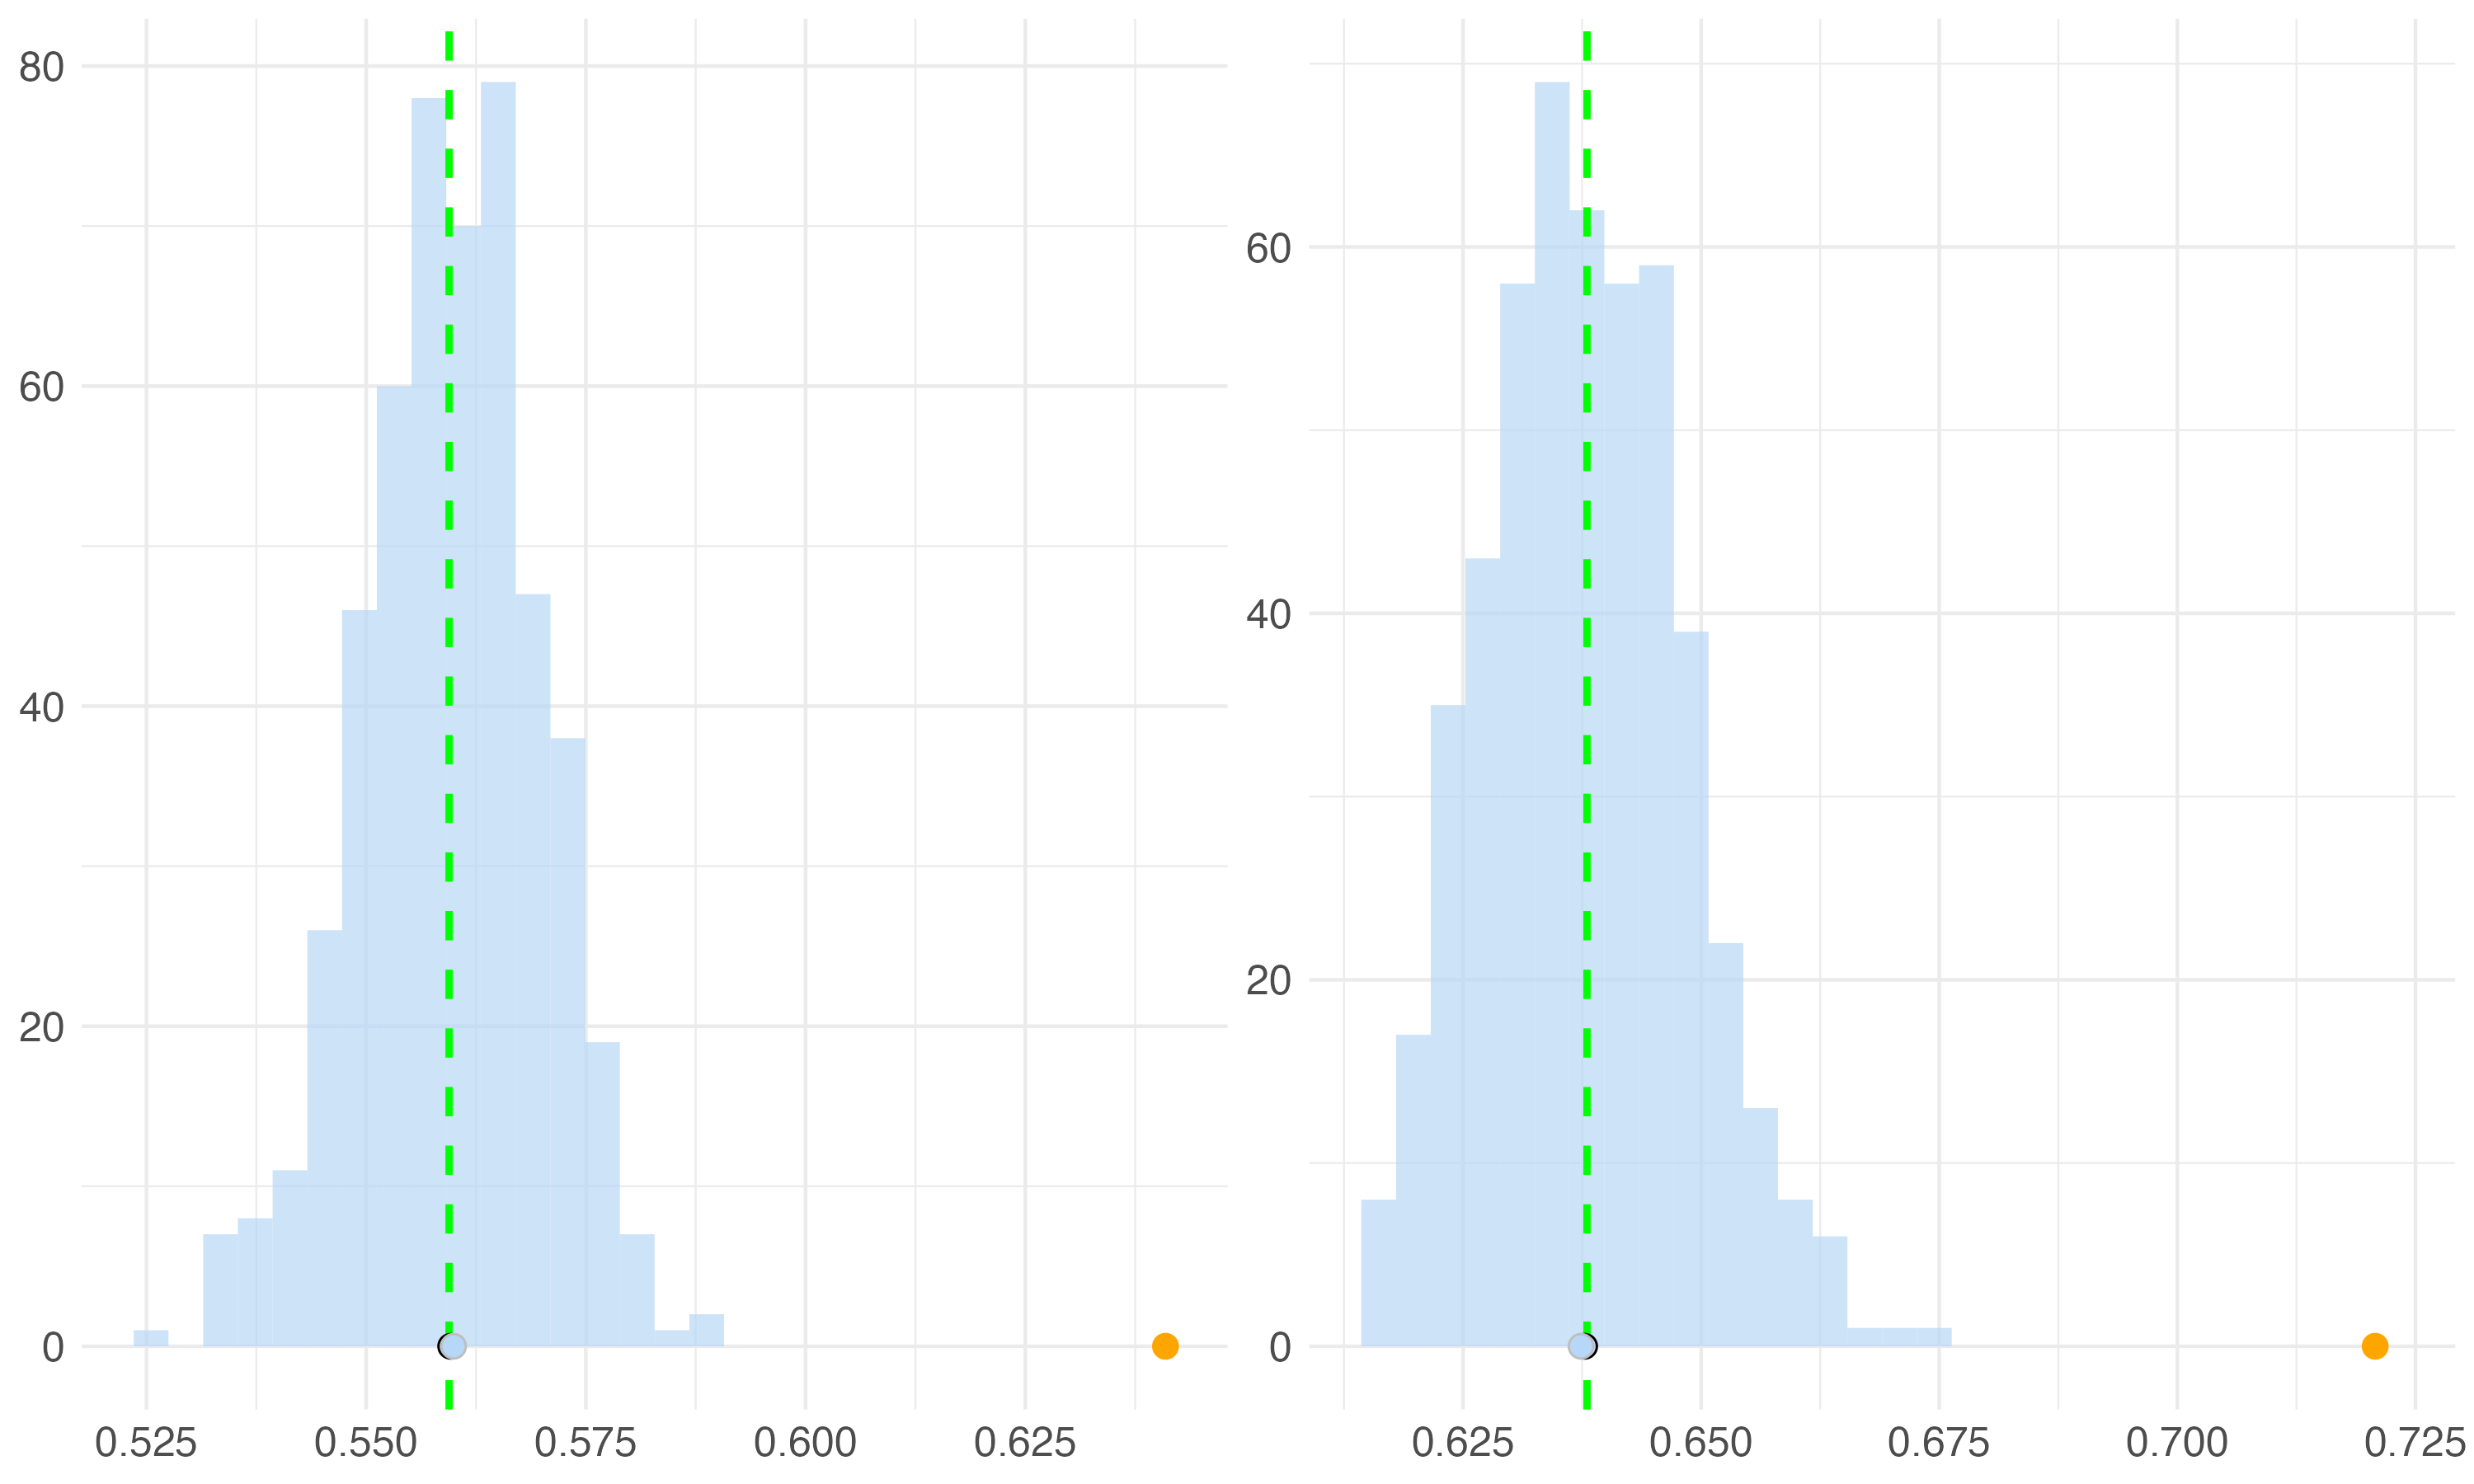
\includegraphics[width=1\linewidth]{Figures/Simulation study/R2_poisson_low_pos.png}
%   \caption{(d) Marginal and conditional $R^2$ estimates for $\rho=0.1$.}
%   \label{fig:r2_poisson_low_pos}
% \end{figure}
% \begin{figure}[H]\ContinuedFloat
%   \centering
%   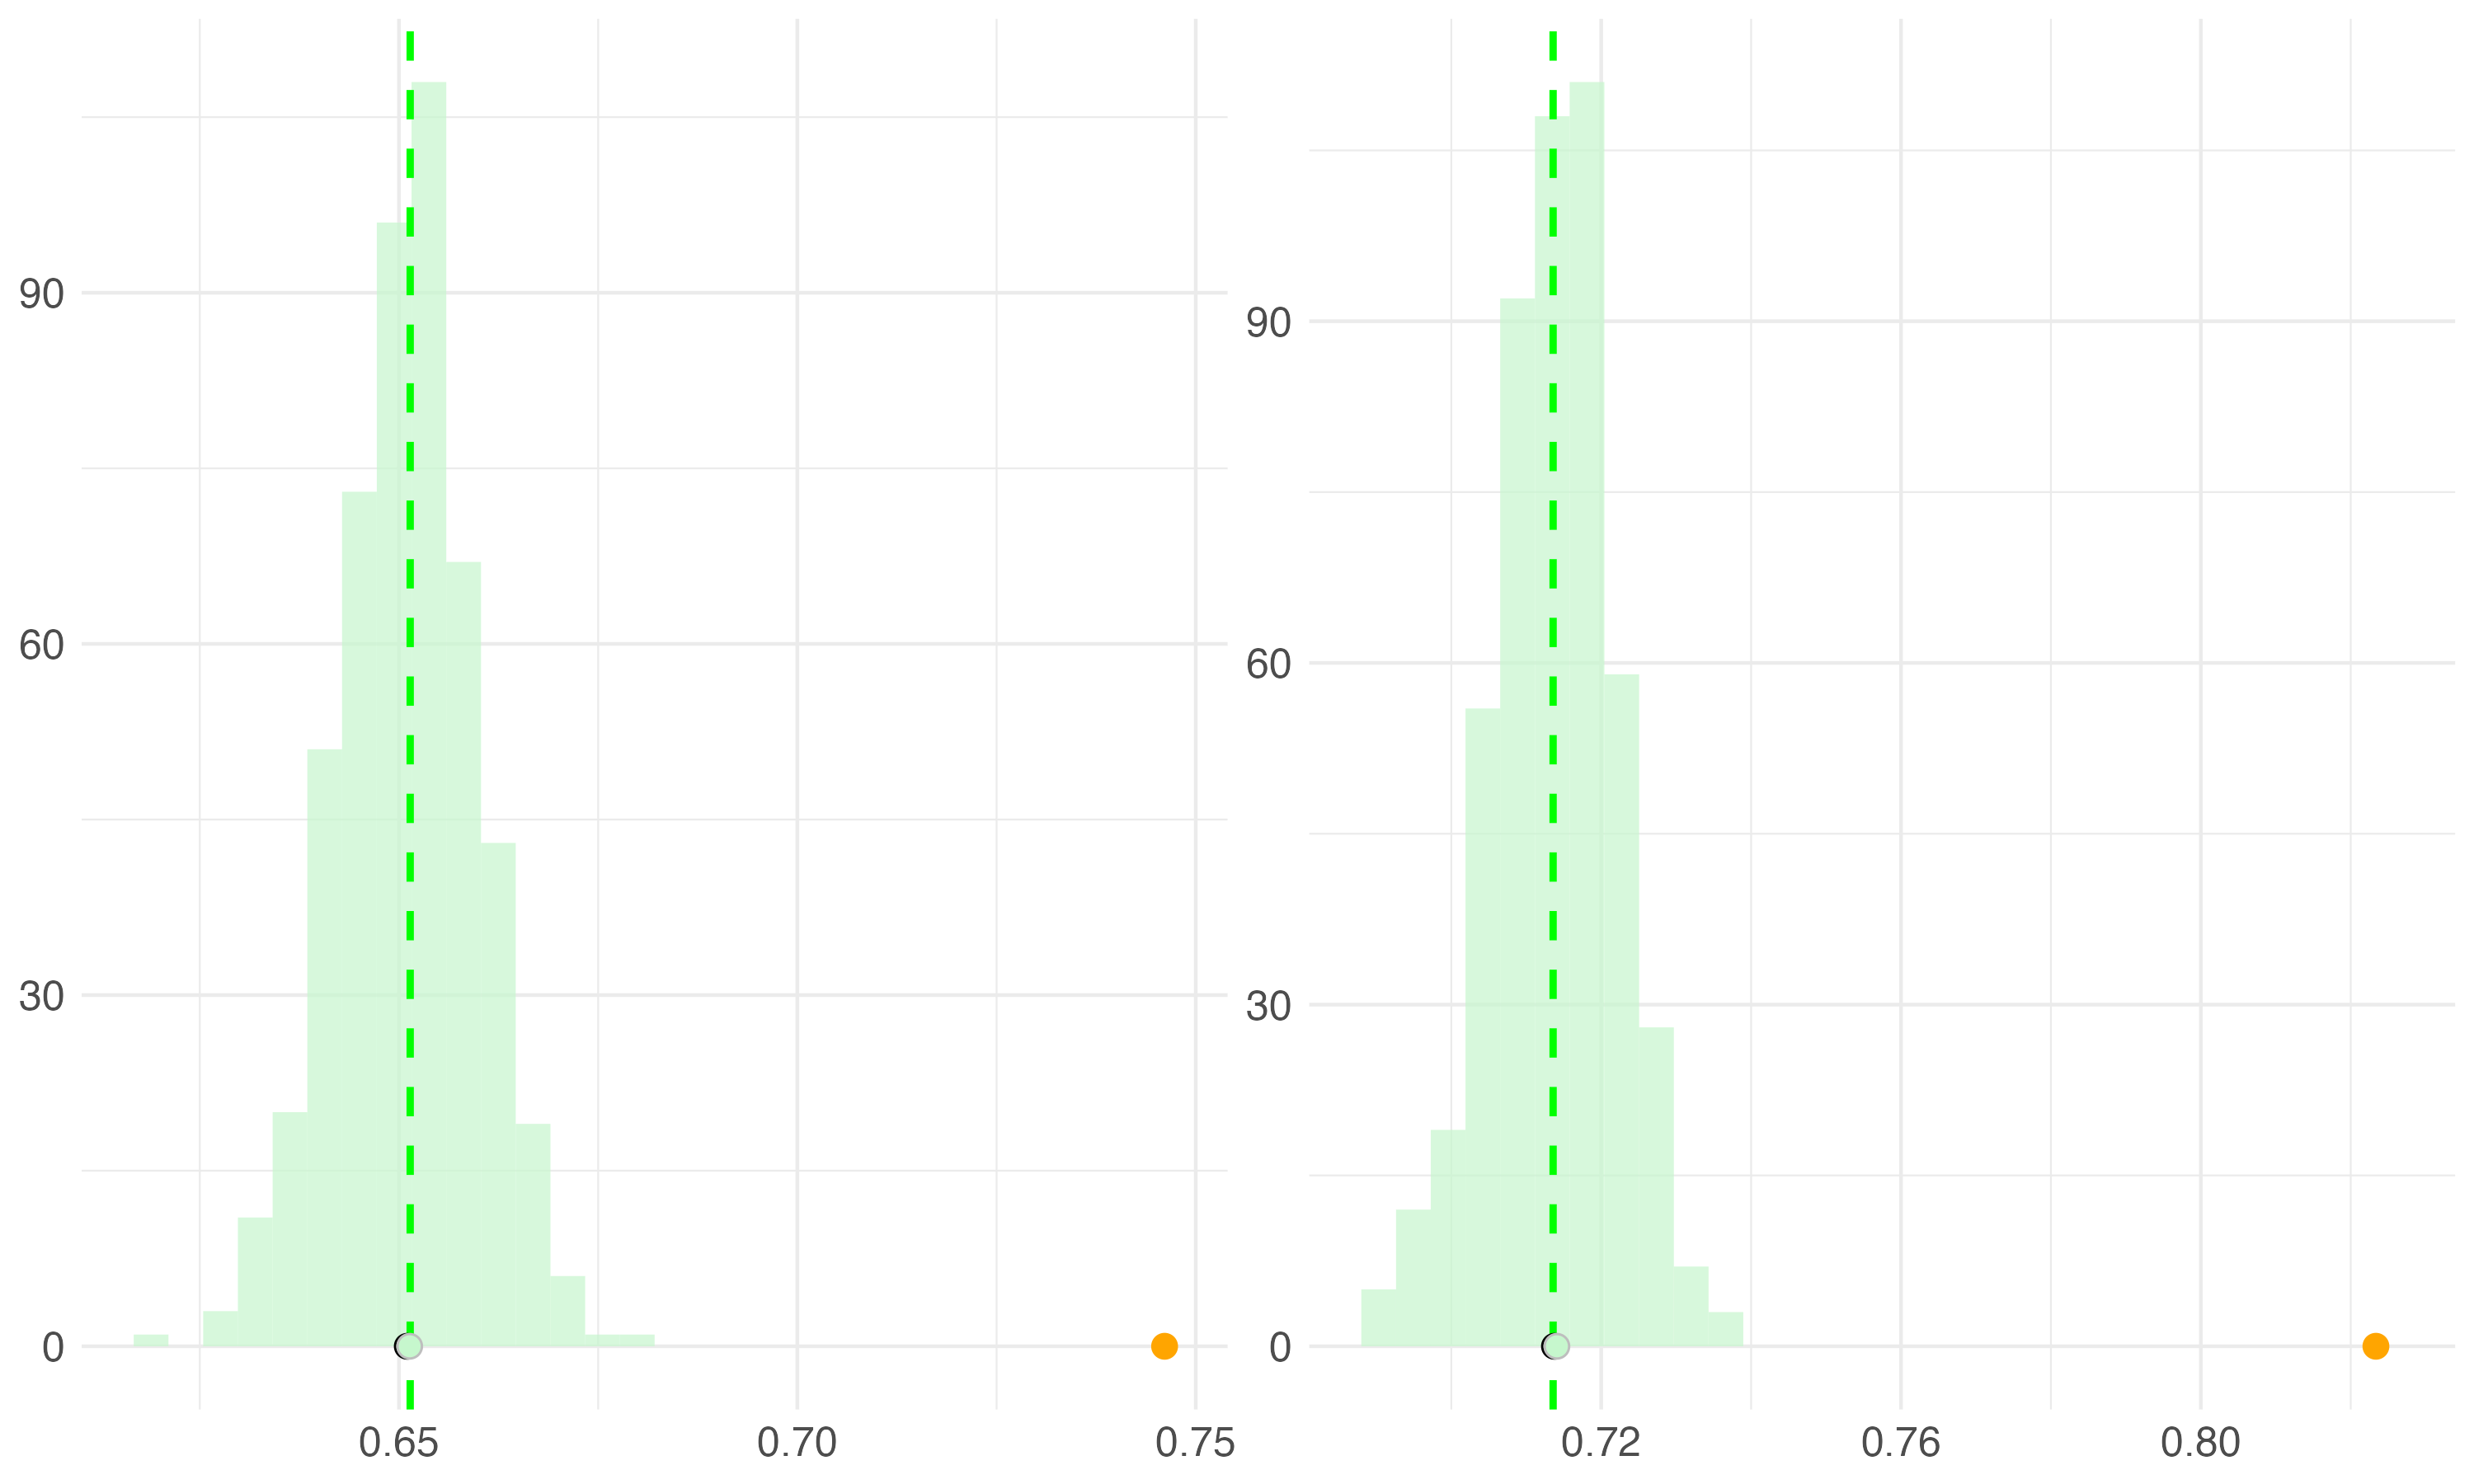
\includegraphics[width=1\linewidth]{Figures/Simulation study/R2_poisson_high_pos.png}
%   \caption{(e) Marginal and conditional $R^2$ estimates for $\rho=0.4$.}
%   \label{fig:r2_poisson_high_pos}
% \end{figure}

\begin{figure}[H]
  \centering
  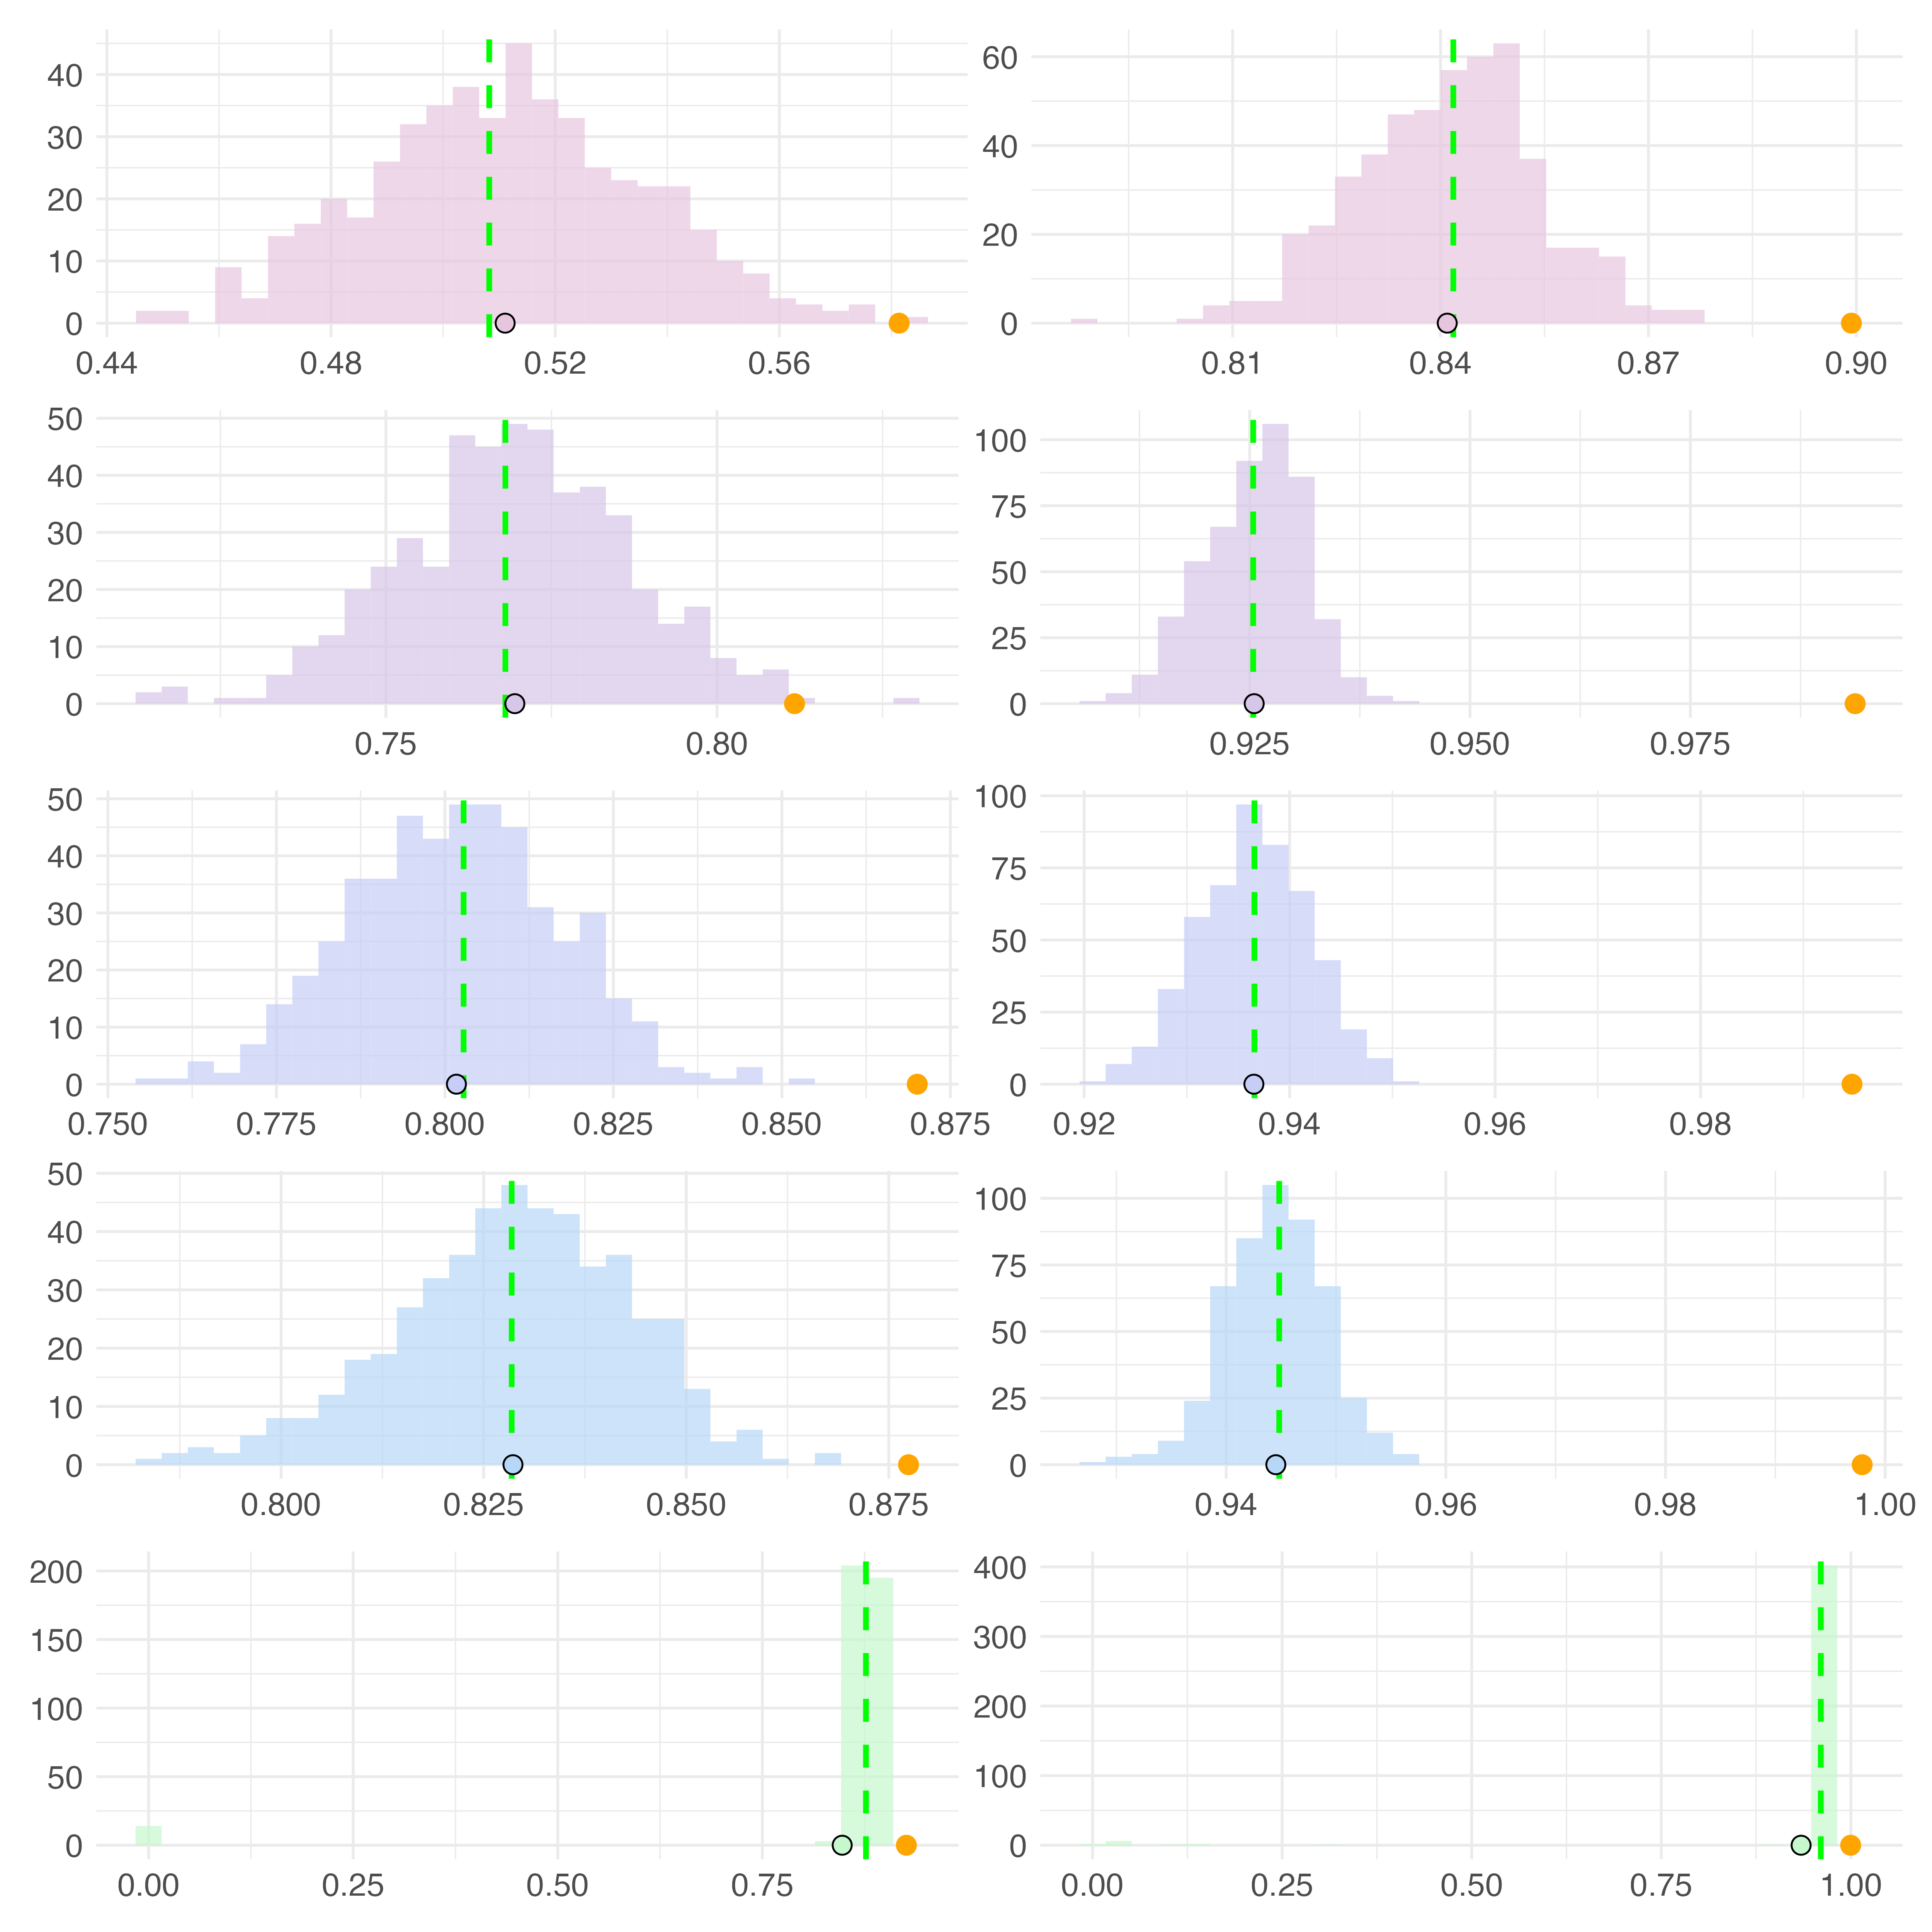
\includegraphics[width=1.1\linewidth]{Figures/Simulation study/R2_combined_poisson.png}
  \caption[Marginal and conditional $R^2$ in Poisson GLMM]{Histograms with the posterior modes of the estimated marginal and conditional $R^2$ from the BVI method for the binomial regression for the different correlation levels $\rho$. The modes are calculated by the Bayesian Variable Importance method from the $N_{\text{sim}}=500$ simulations in the simulation study. The expected values are displayed as vertical green lines, and can be found in \Cref{table:r2values}, while the orange dot denotes the estimate from the \texttt{rptR} package. The mean value of the $R^2$ values for all simulations is marked with a circle at the bottom of each histogram.}
  \label{fig:r2_combined_poisson}
\end{figure}


% \begin{figure}[H]
%   \centering
%     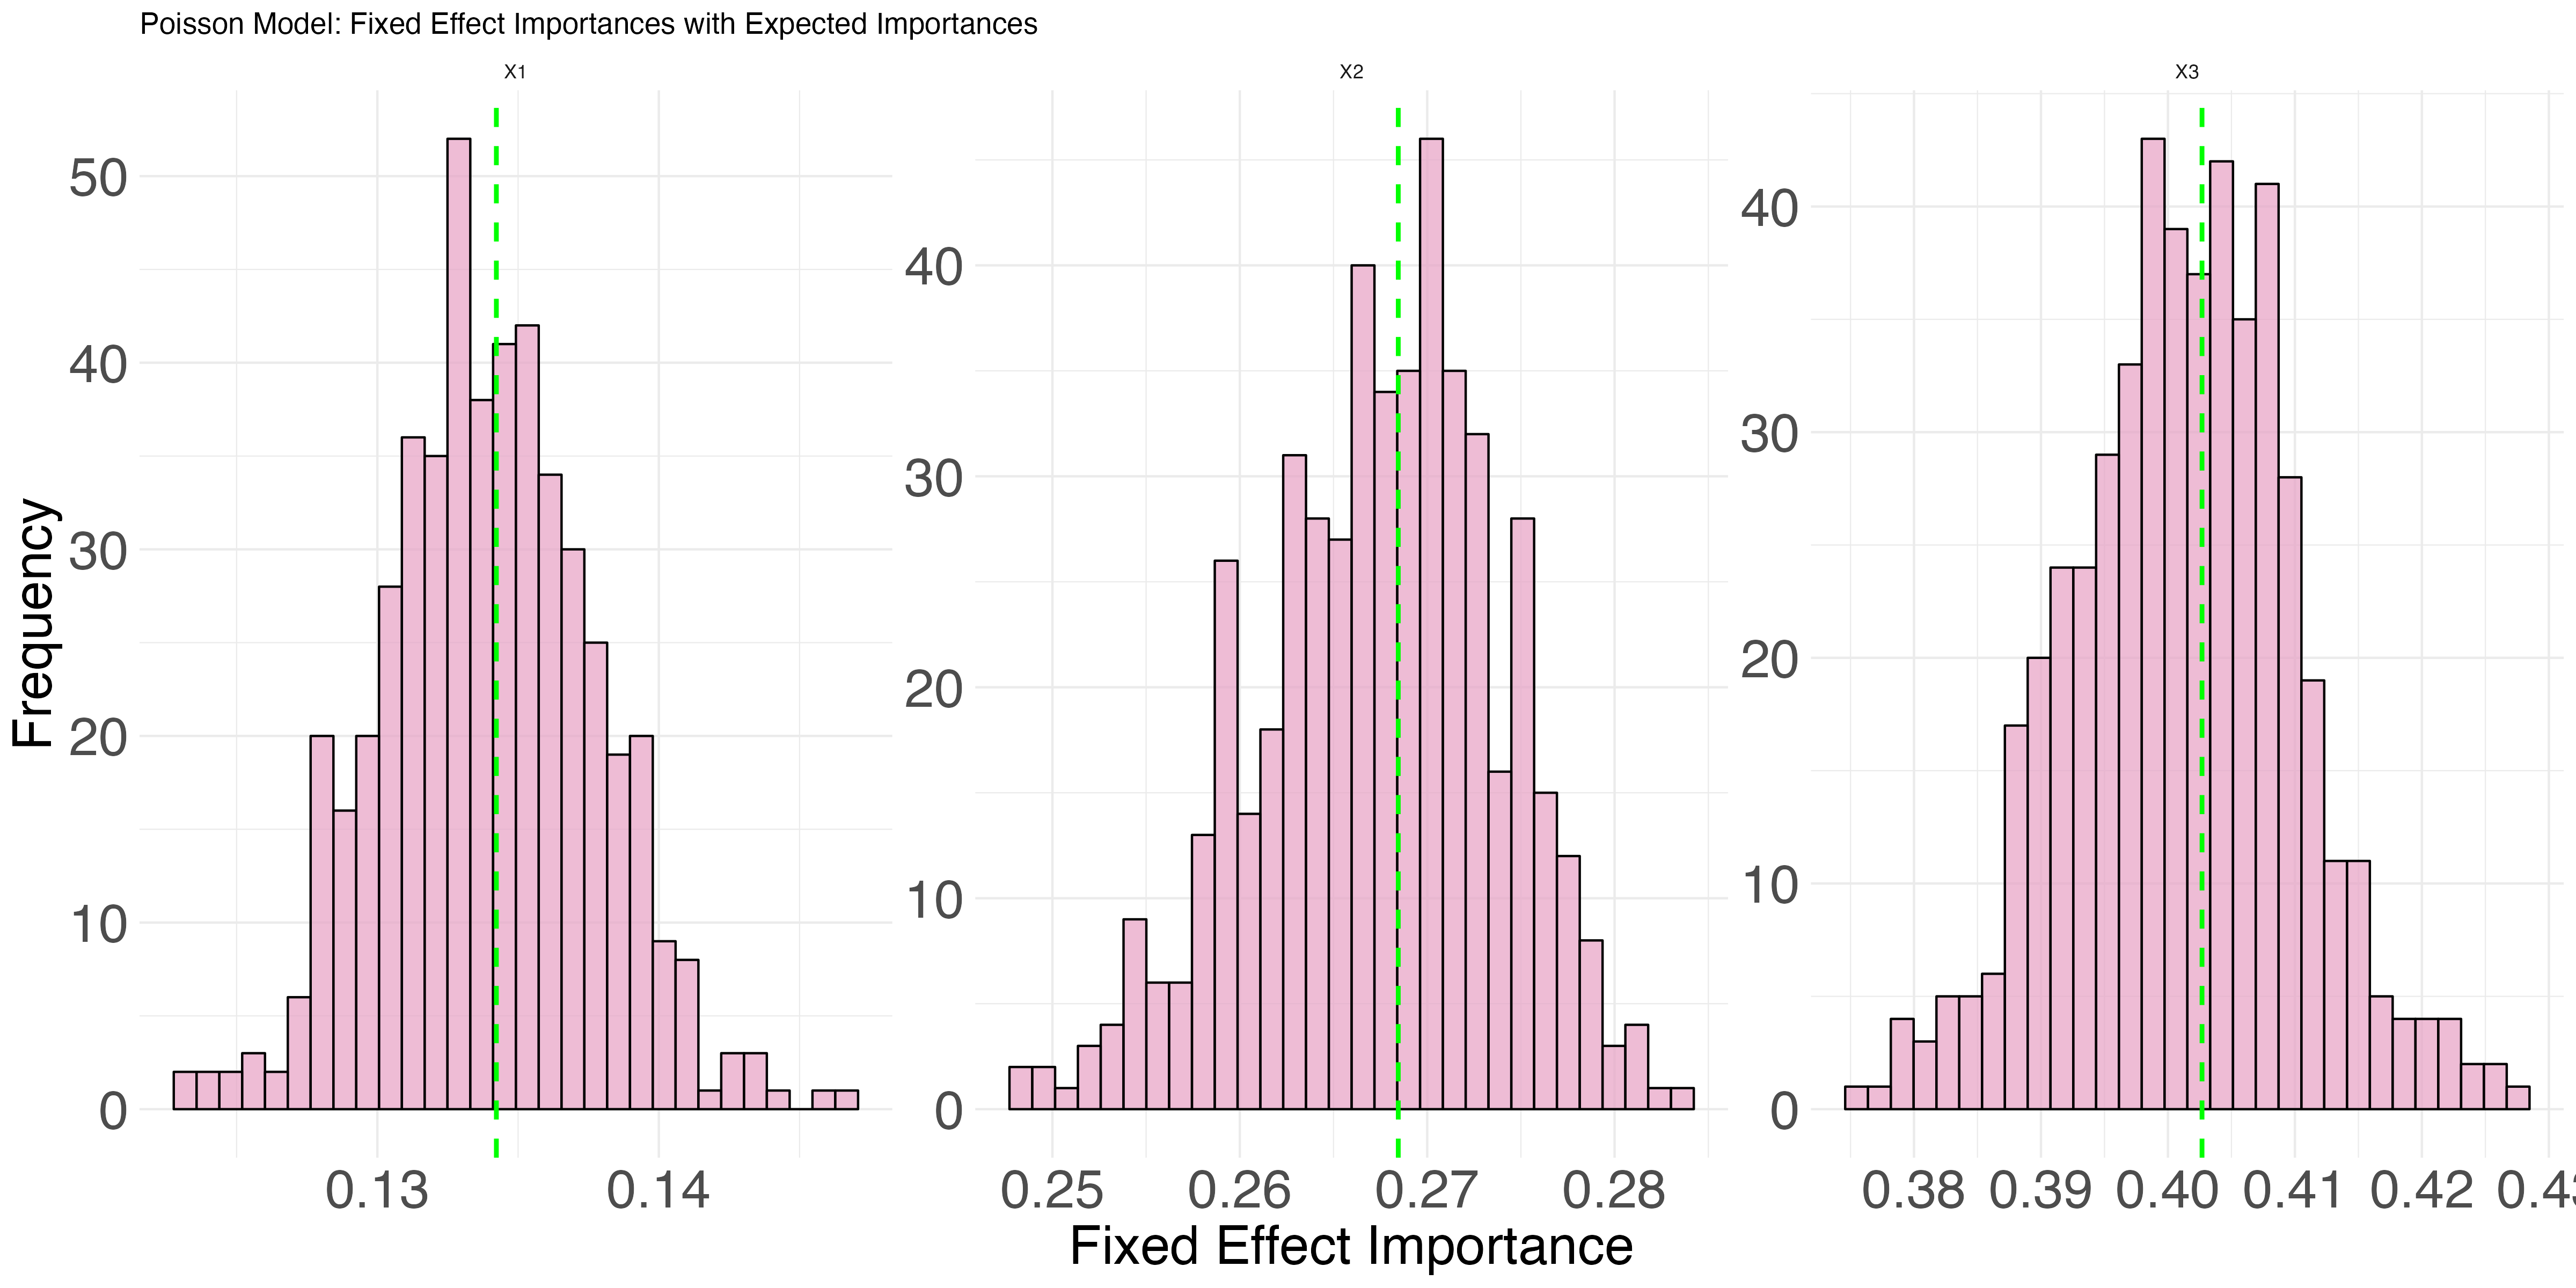
\includegraphics[width=1\linewidth]{Figures/Simulation study/Fixed_poisson.png}
%     \caption{Relative importance of fixed effects for poisson GLMM}
%     \label{fig:relimp_poisson_fixed}
% \end{figure}
% \begin{figure}[H]\ContinuedFloat
%   \centering
%   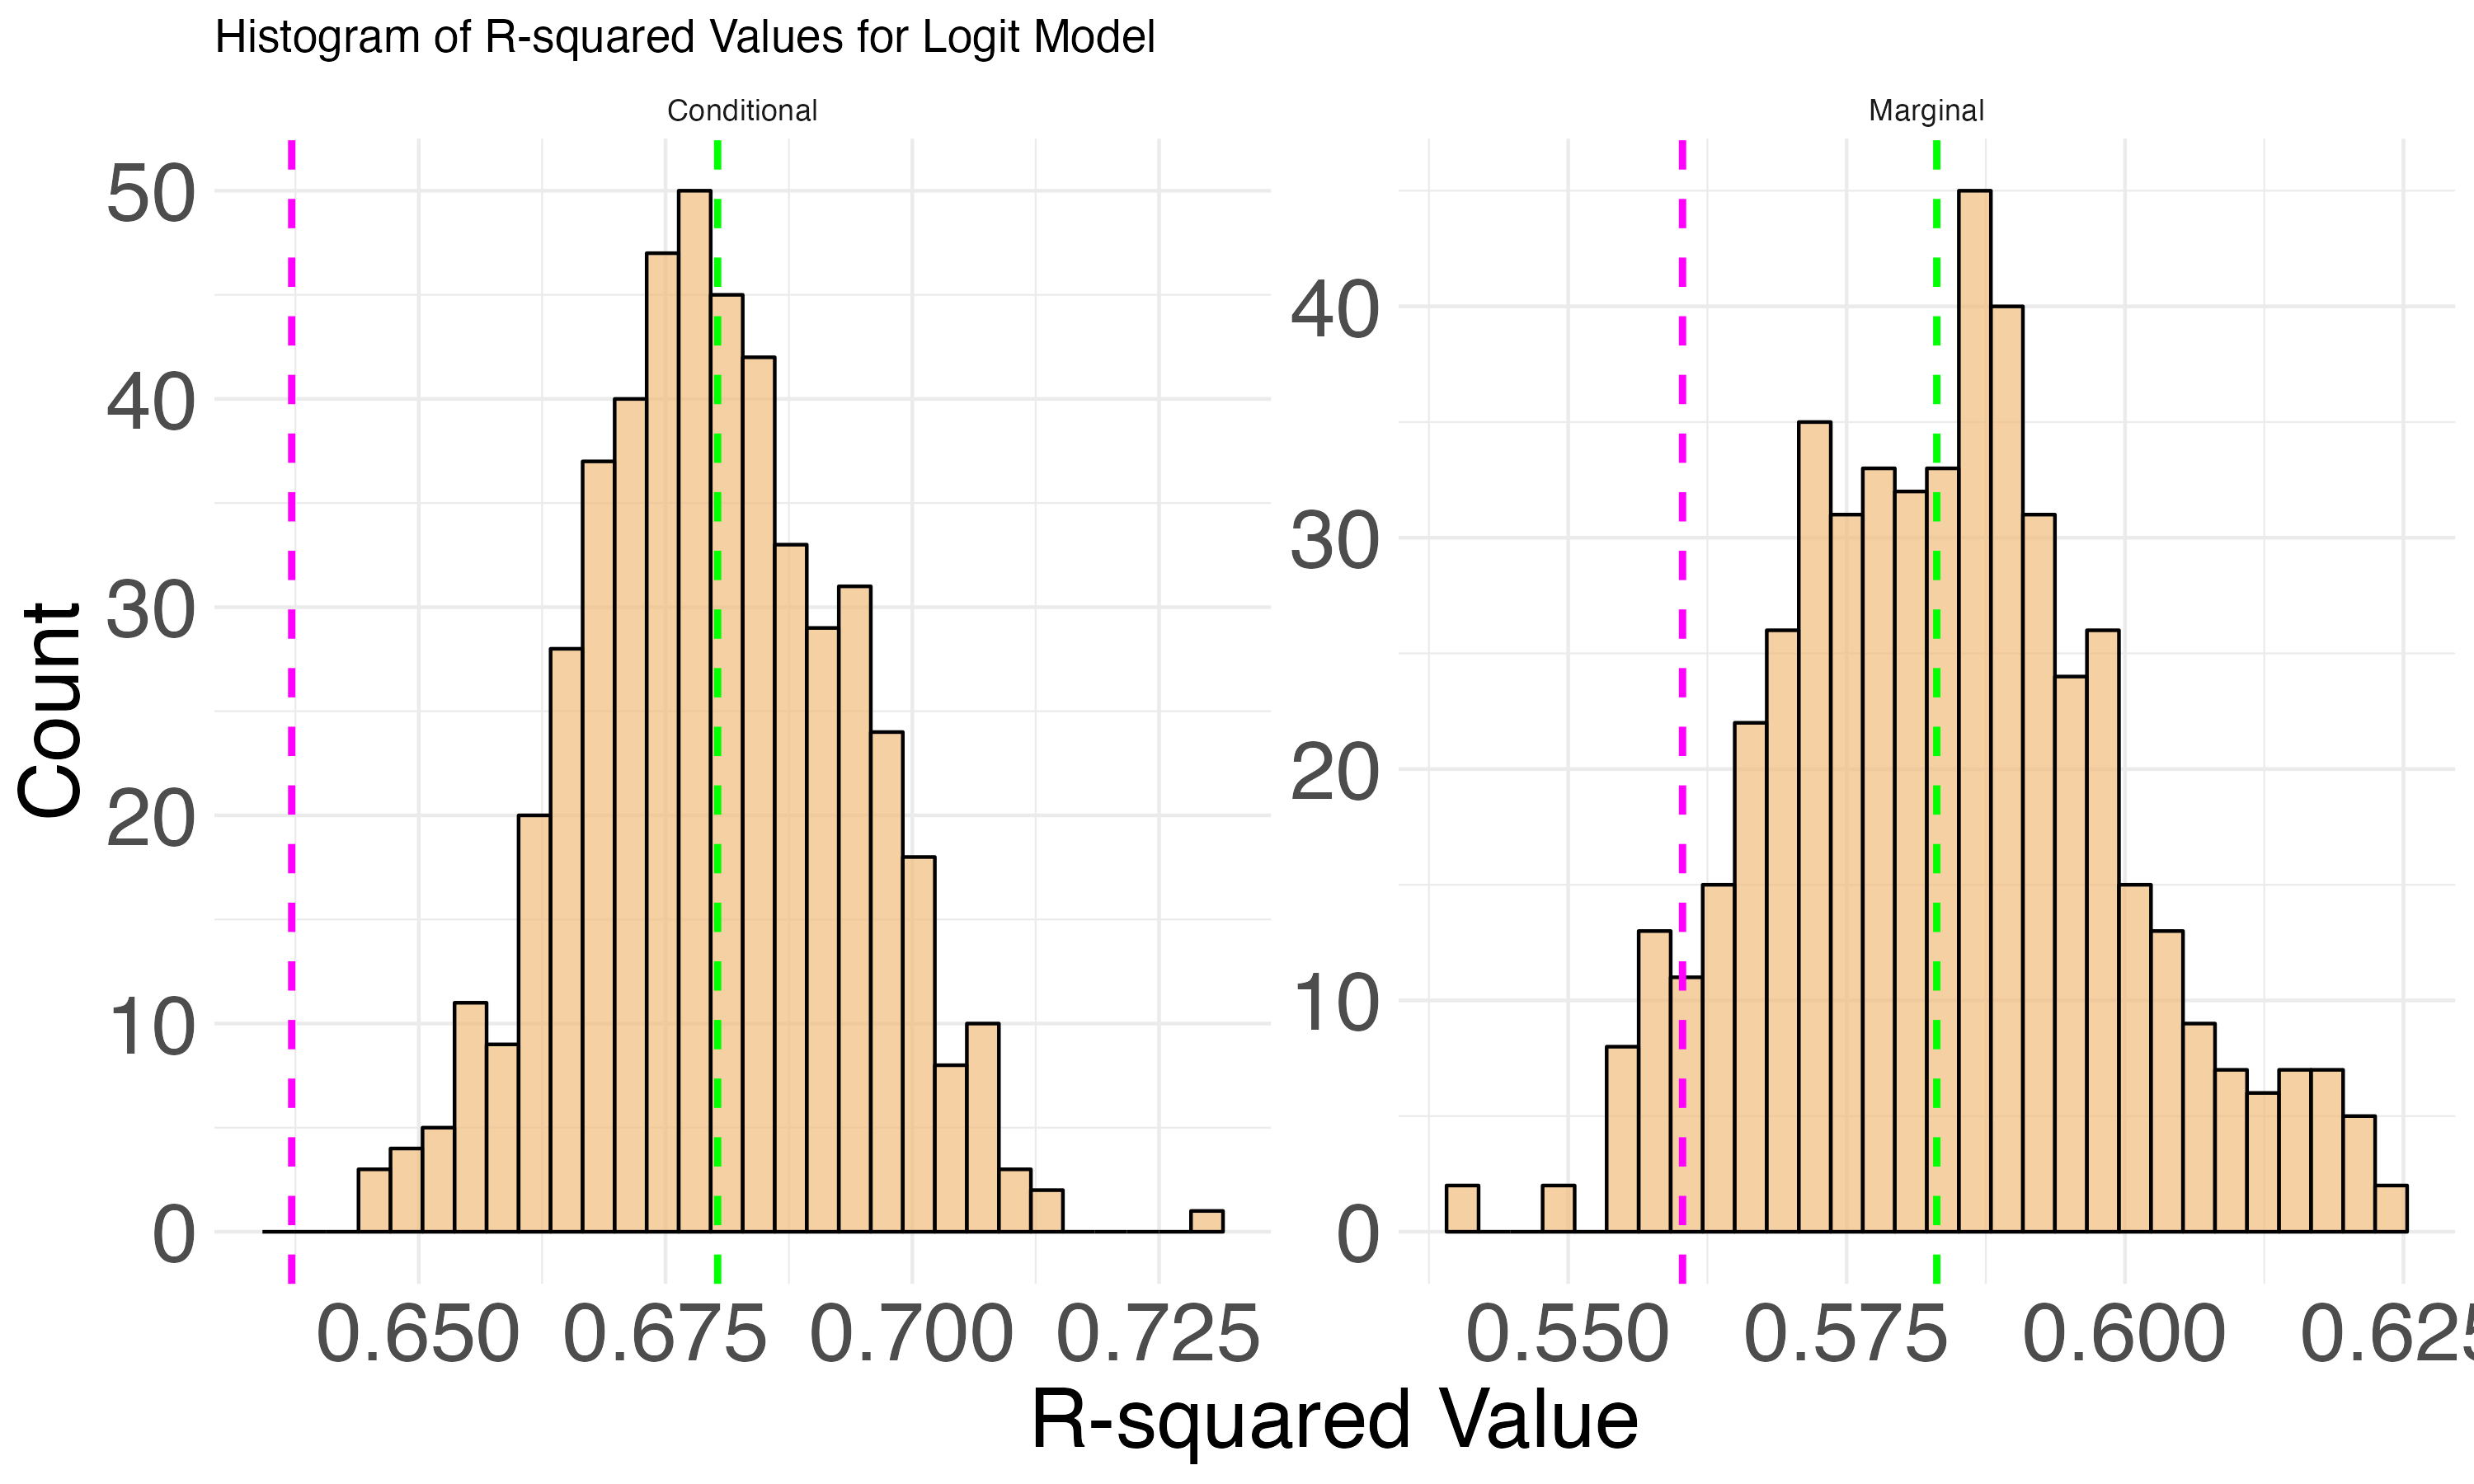
\includegraphics[width=1\linewidth]{Figures/Simulation study/R2_logit.png}
%   \caption{Conditional and marginal $R^2$ for poisson GLMM. The magenta line is Stoffel, green line is expected importance}
%     \label{fig:relimp_poisson_R2}
% \end{figure}


\section{Case study with \texttt{rptR} package}
% \begin{figure}[H]
%     \centering
%       \includegraphics[width=0.7\linewidth]{Figures/Stoffel Comparison/Heritability_colour_Binomial.png}
%       \caption{Heritability of colour of male beetles from Stoffel}
%       \label{fig:heritability_colour_Binomial}
%   \end{figure}
%   \begin{figure}[H]\ContinuedFloat
%     \centering
%     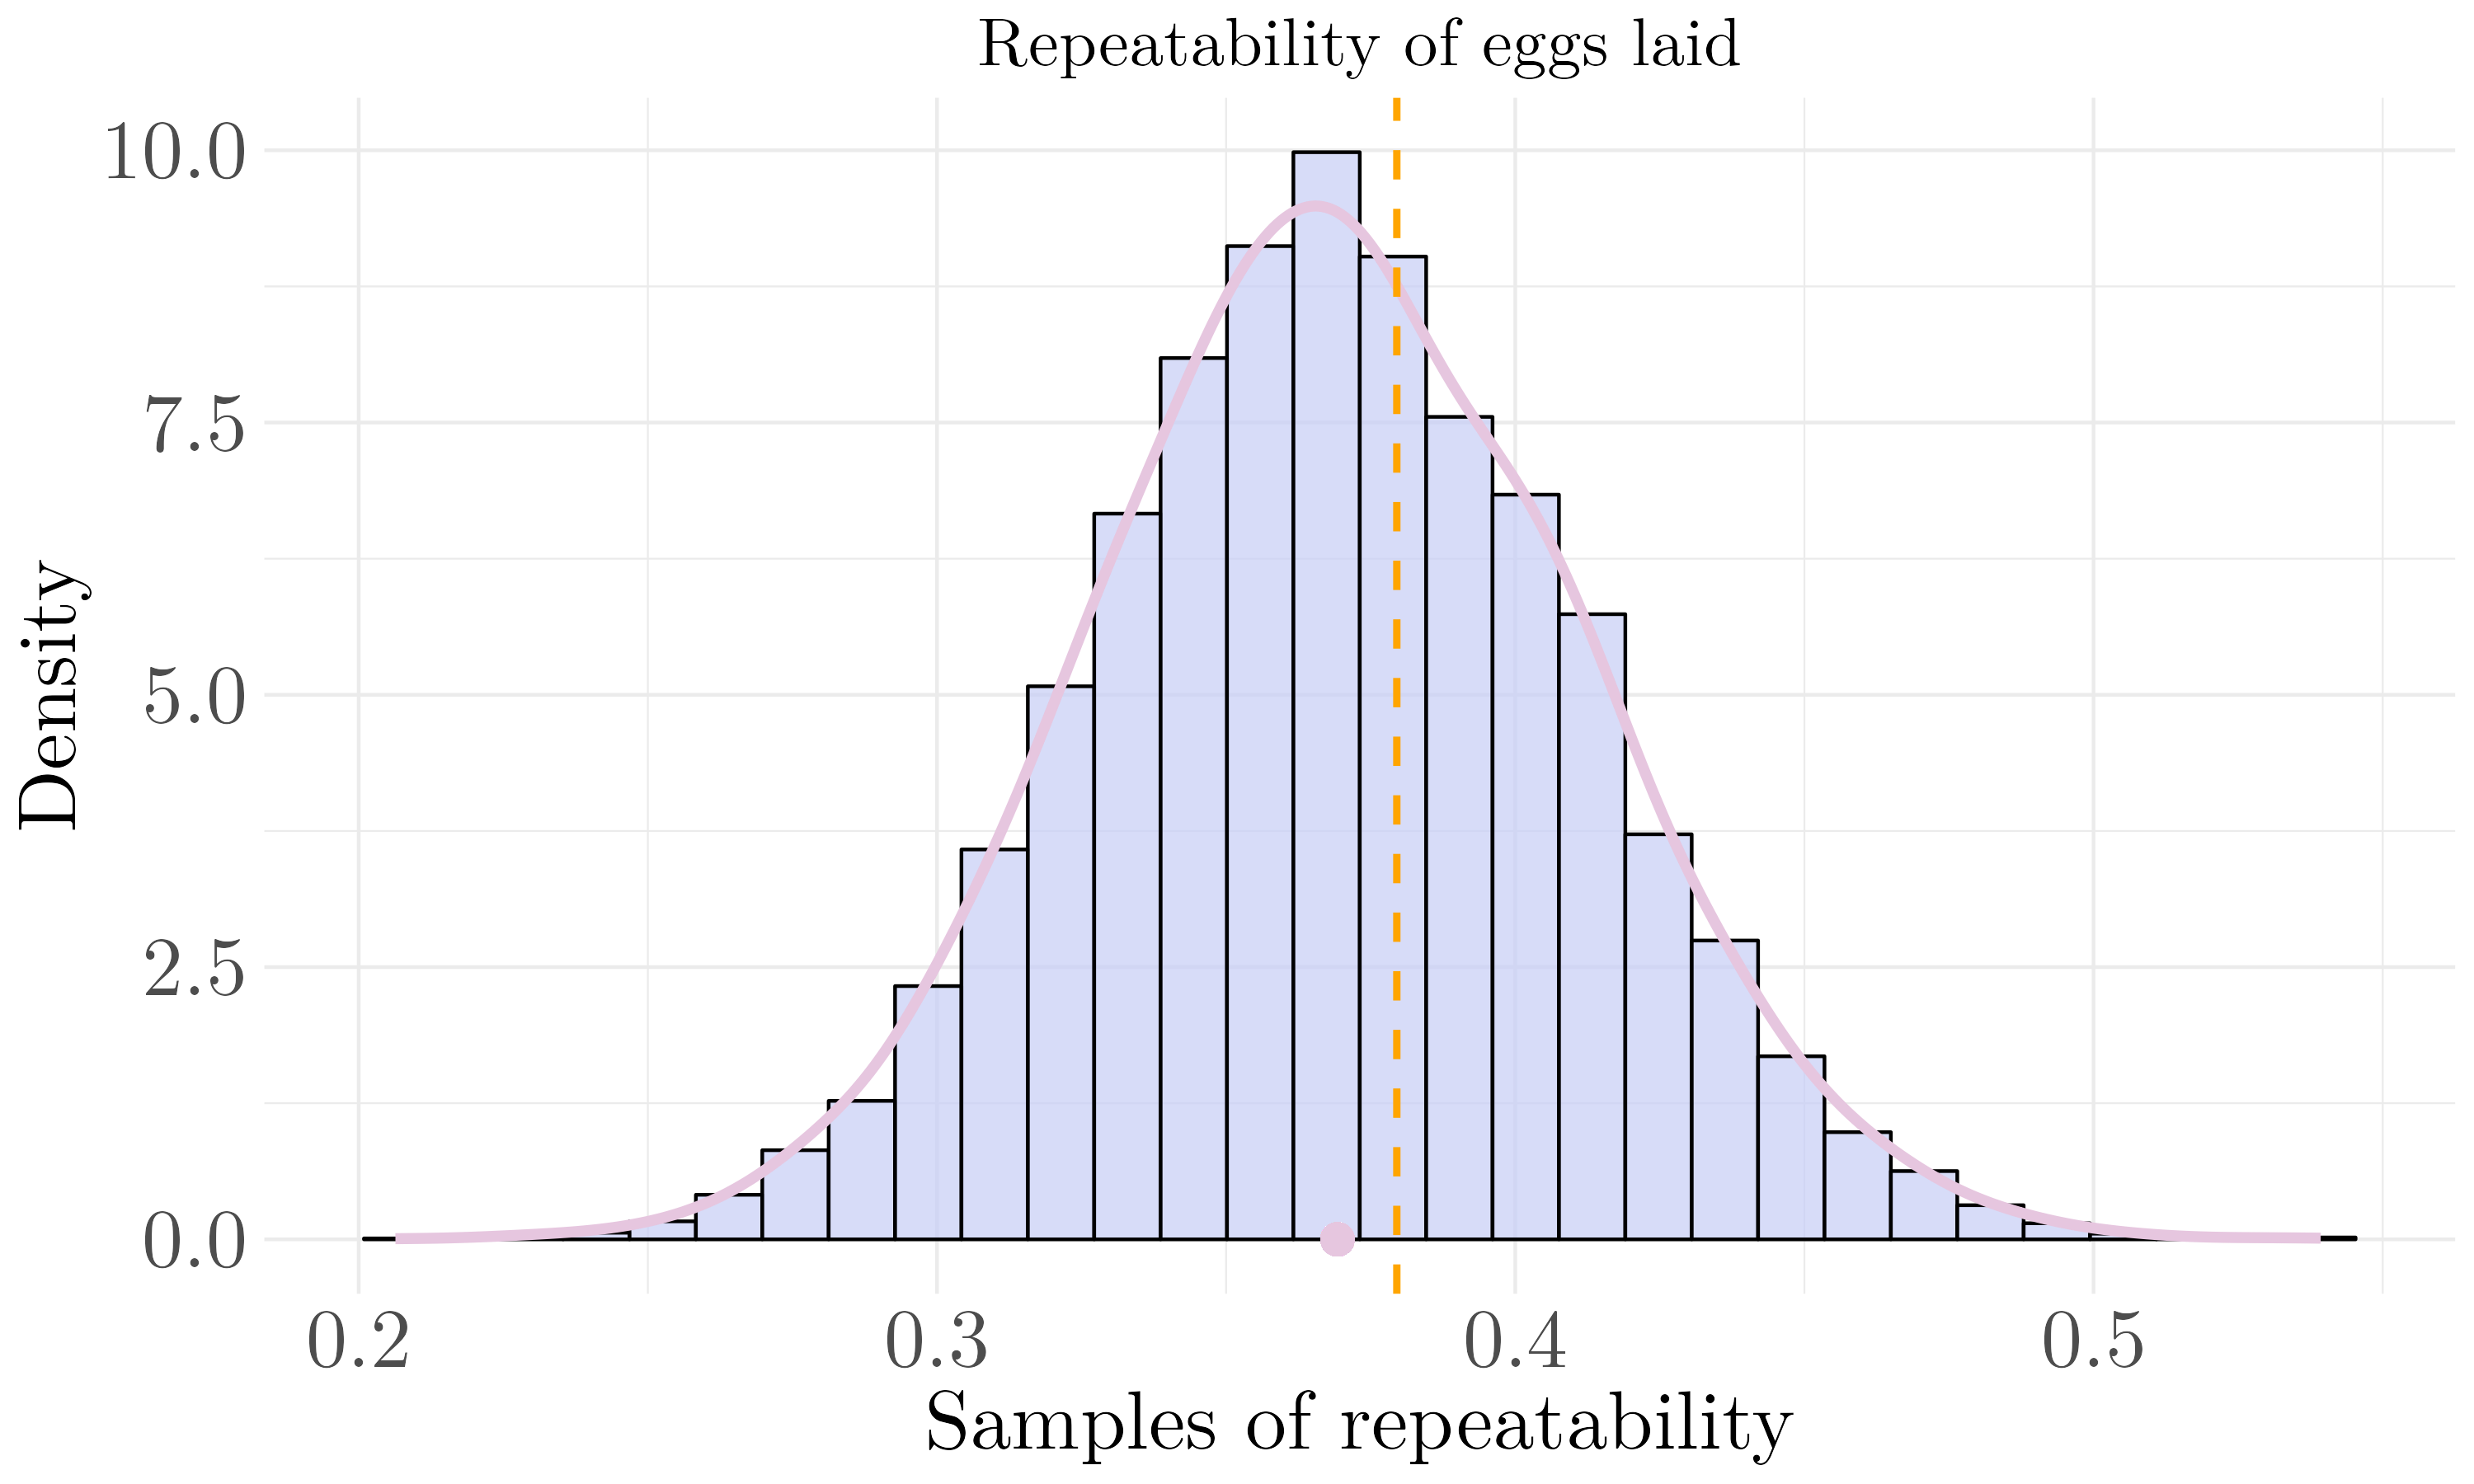
\includegraphics[width=0.7\linewidth]{Figures/Stoffel Comparison/Heritability_egg_poisson.png}
%     \caption{Heritability of eggs laid by female beetles from Stoffel}
%       \label{fig:heritability_egg_poisson}
%   \end{figure}
To further assess our method, a comparison to the vignette for the \texttt{rptR} was made. The package described in this vignette estimates the repeatability of phenotypic traits, which for some definitions coincide with heritability and therefore can be seen as a special case of variable importance. Thus, we were able to apply the Bayesian Variable Importance method and compare the results. No expected results were available, and so we can only compare our method to the results made by the authors of the vignette. It should however be noted, that the \texttt{rptR} package returns the marginal $R^2$ as the only measure of importance for the fixed effects, whereas our method directly decomposes this value and assigns a share to each fixed effect. To obtain uncertainty estimates in the likelihood framework, Stoffel, Nakagawa and Schielzeth have built in bootstrap functionality. This is used in our comparison, to evaluate computational complexity and confidence intervals.
\\
\\
The repeatability of the color of male beetles is modelled by a binomial GLMM with binary outcome and logit-link. We use the same formulation as in the model \texttt{rep11} from the vignette \citep{Stoffel2017rptR}, with the parameter \texttt{adjusted=FALSE}. We see that the sampled posterior distribution of repeatability (\Cref{fig:heritability_colour_Binomial}) from the Bayesian Variable Importance method is centered around a mean of $0.193$, which is very similar to the estimate by Stoffel which is $0.196$. The obtained distribution appears unimodal, with the mode and mean aligning closely. Perhaps a slightly longer tail on the right side can be observed. From $10^3$ bootstrap samples, the \texttt{rptR} estimates a $95\%$ confidence interval of $[0.051, 0.338]$, which is a bit larger than our estimated $95$th percentile of $[0.114, 0.280]$. In terms of computation time, the Bayesian Variable Importance method used $6$ seconds to obtain the model fit and $10^4$ samples, whereas the \texttt{rptR} package used $66$ seconds to obtain the model fit and the same number of bootstrap samples.
\begin{figure}[H]
  \centering
  % First row
  \includegraphics[width=1\linewidth]{Figures/Stoffel Comparison/Heritability_colour_Binomial.png}
  \caption[Estimated repeatability of color in male beetles]{Histogram with repeatability values sampled from the posterior distribution for the color of male beetles from the BVI method, with the mean of the samples denoted by a pink circle. The estimate from the \texttt{rptR} package marked as a dashed line with orange color.}
  \label{fig:heritability_colour_Binomial}
\end{figure}
% We see that the approximated distribution from the BVI method is centered a bit to the right of the point estimate from \texttt{rptR}. The stochasticity of the BVI method makes it so that the distributions return will vary based on what seed was made to generate the results. Therefore, we expect to see a difference between the centering of the distribution and point estimates. 
\noindent To estimate the repeatability of the number of eggs laid by female beetles, we use a Poisson GLMM with log-link. The model used in our method corresponds to \texttt{rep9}, but as is described in the vignette after fitting \texttt{rep9}, we set the option \texttt{expect="latent"} so that the method calculates the distributional variance as in \Cref{table:1}. This corresponds to the recommendations of \citet{nakagawa2017} as previously mentioned. Likewise, this model is estimated from the \texttt{rptR} package with \texttt{adjusted=FALSE}. From the plotted samples of posterior repeatability of eggs laid (\Cref{fig:heritability_eggs_poisson}), we see a very similar distribution as that of the binomial color model. The distribution is symmetric and centered around a mean of $0.359$. Further, the estimate from the \texttt{rptR} model is $0.380$ with a confidence interval of $[0.131, 0.542]$, compared to our $95$th percentile of $[0.278, 0.445]$. The $10^3$ bootstrap samples and model fit for the \texttt{rptR} package took $2$ minutes and $13$ seconds, whereas the BVI method used $8$ seconds to obtain the model fit and $10^4$ samples.
% \begin{figure}[H]
%   \centering
%   \begin{subfloat}{0.49\linewidth}
%       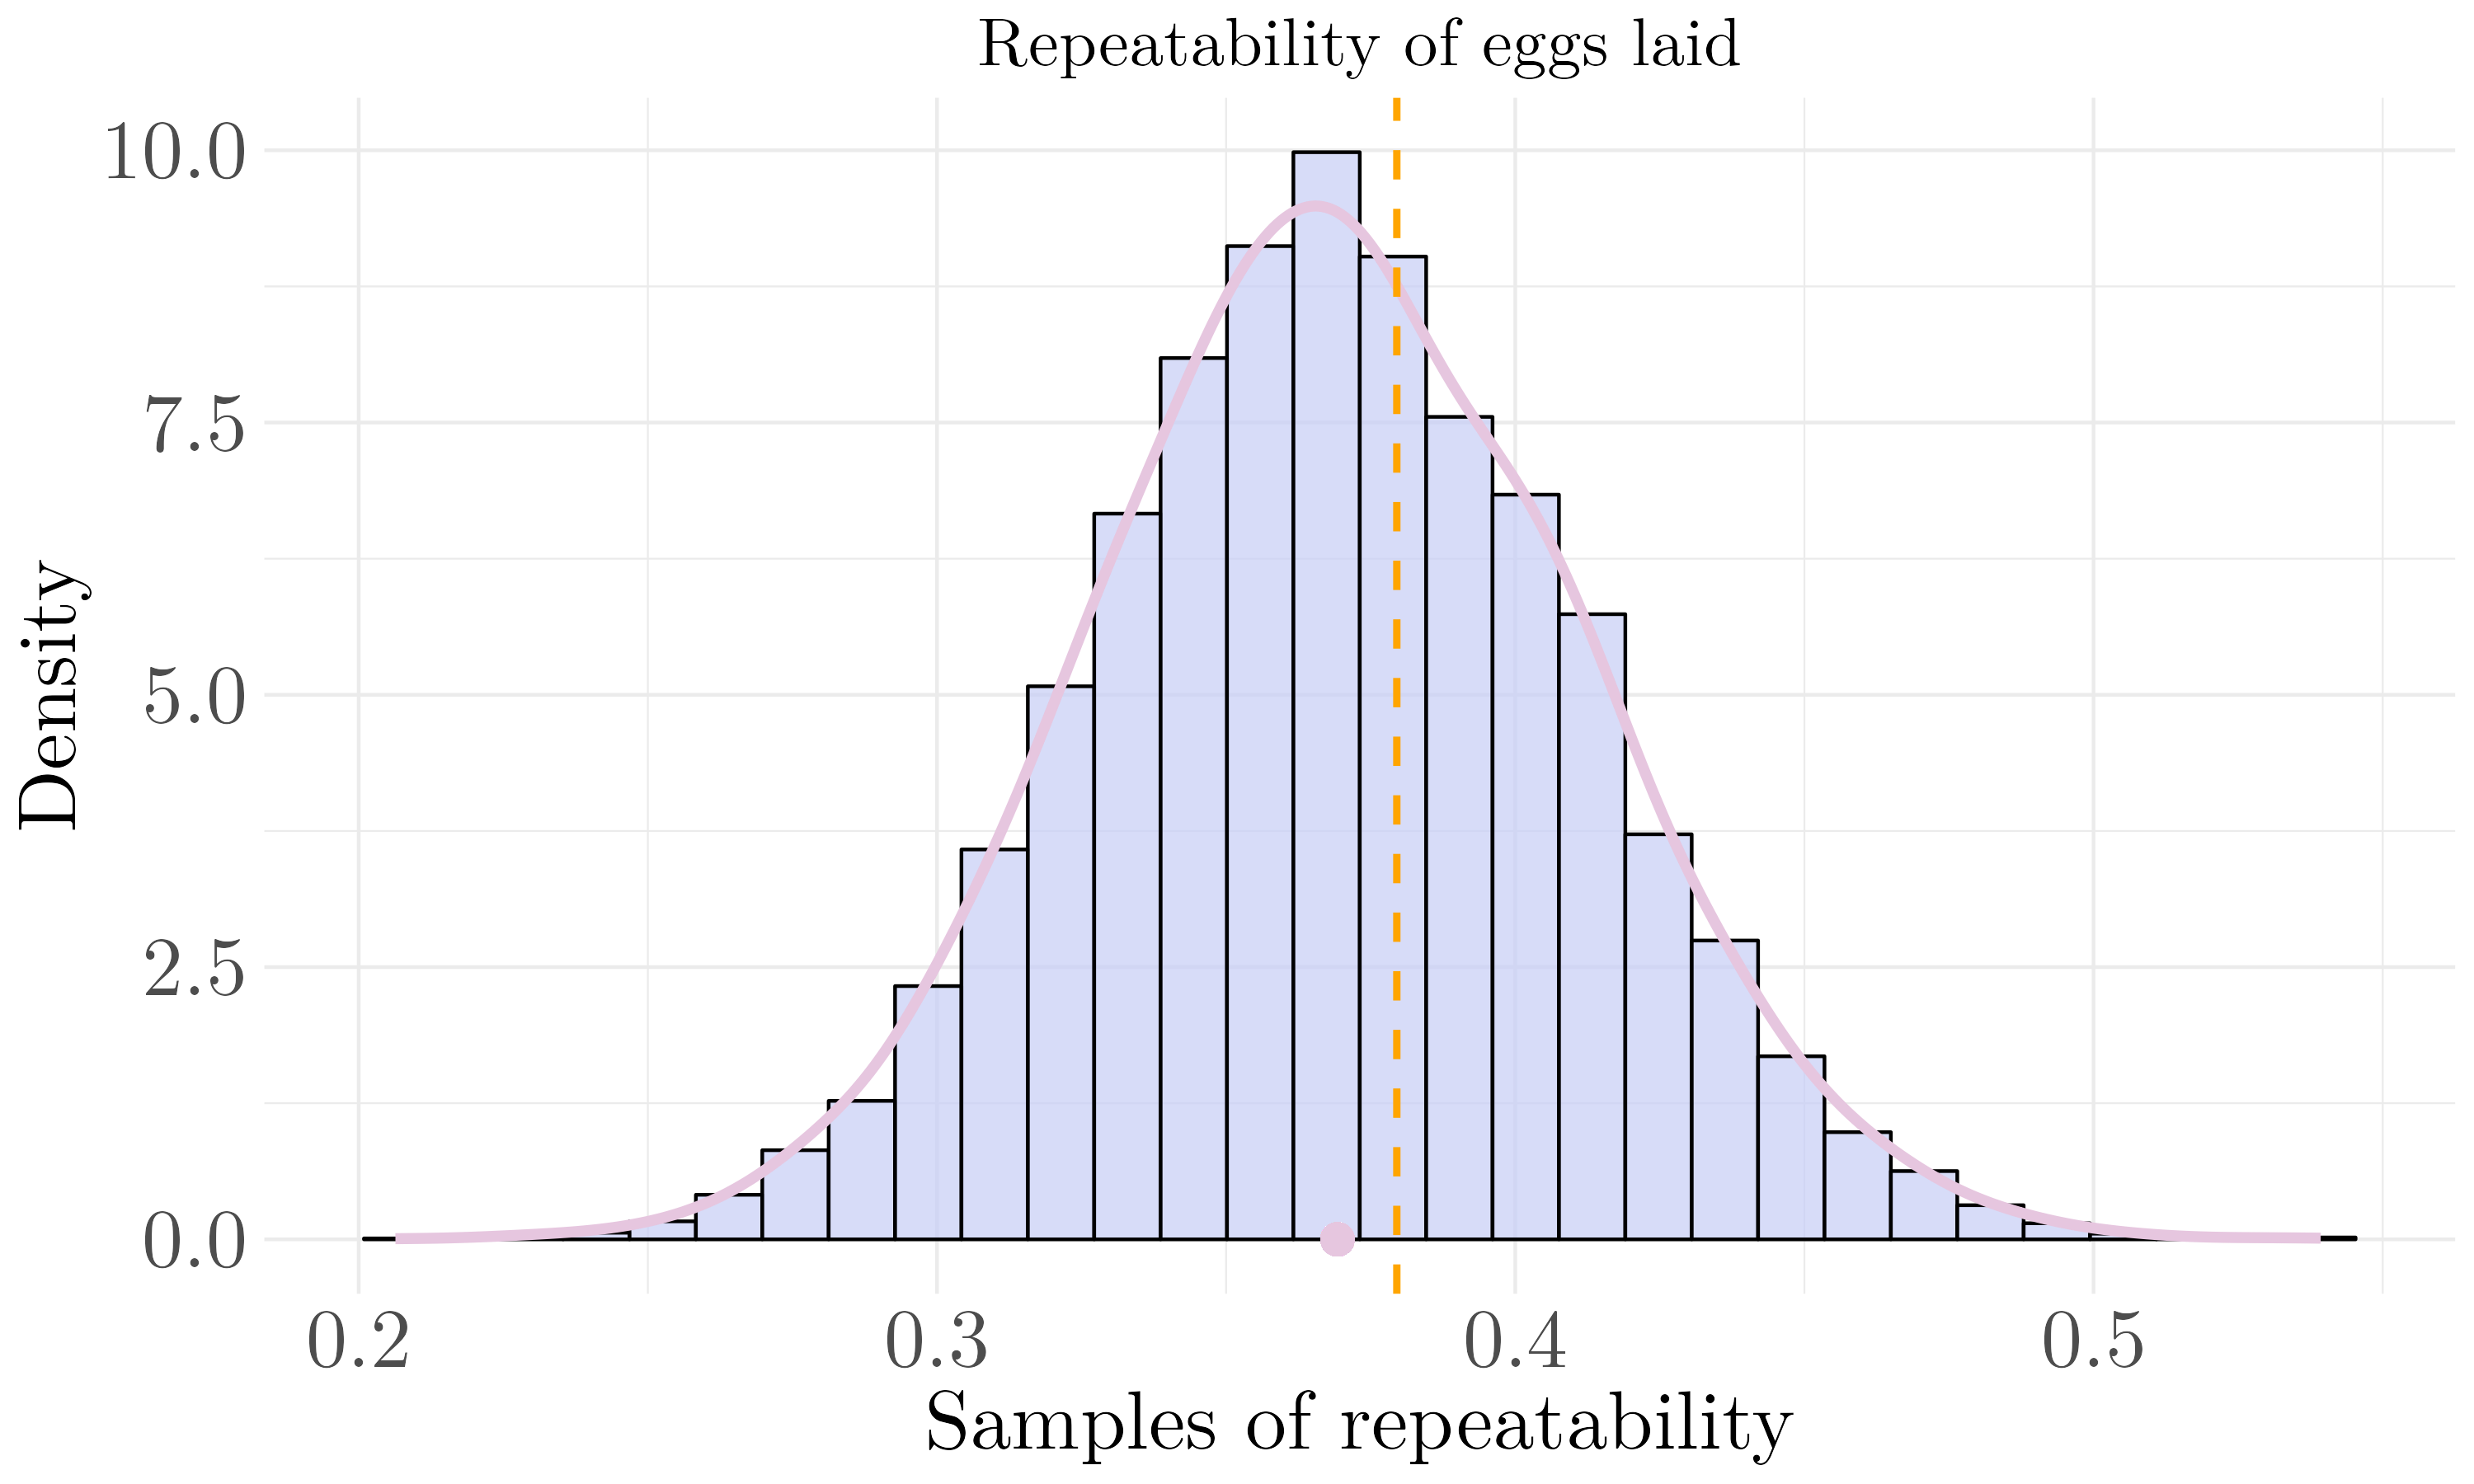
\includegraphics[width=\linewidth]{Figures/Stoffel Comparison/Heritability_egg_poisson.png}
%       \caption{Heritability of eggs laid by female beetles from BVI}
%       \label{fig:heritability_egg_poisson}
%   \end{subfloat}
%   \hfill
%   \begin{subfloat}{0.49\linewidth}
%       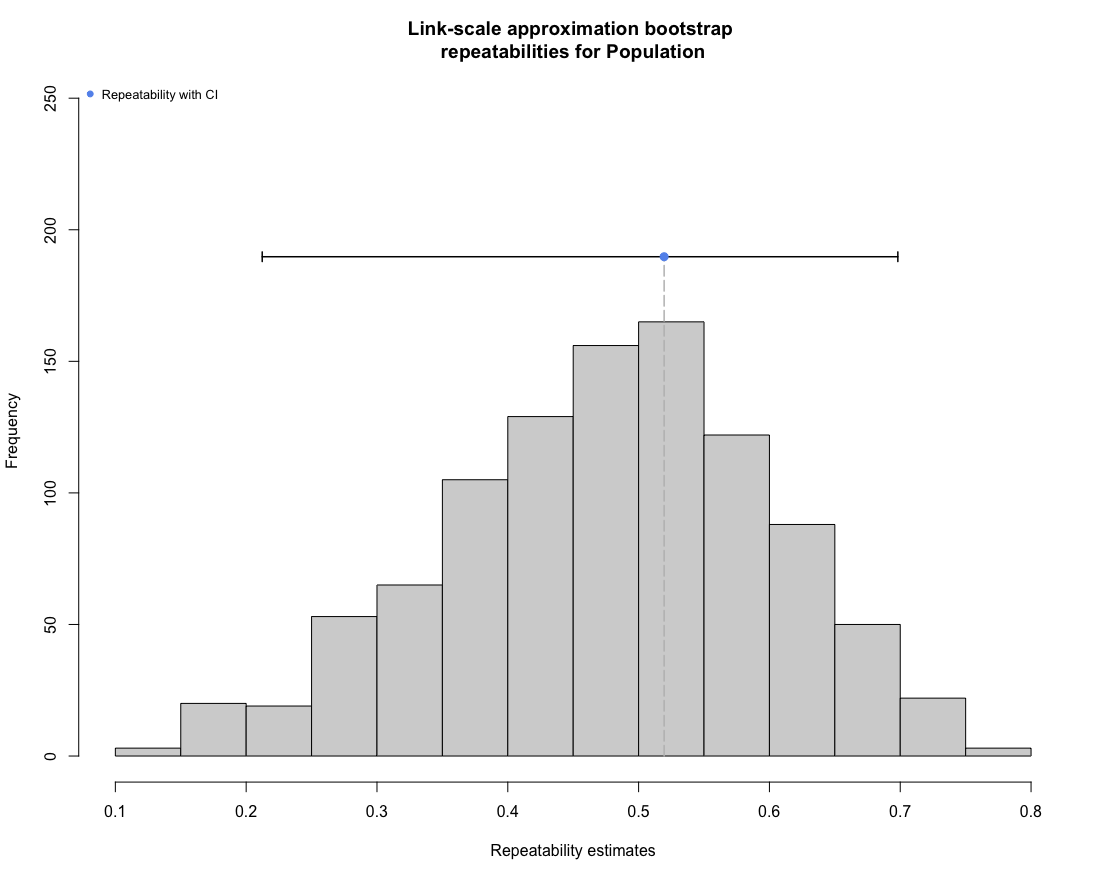
\includegraphics[width=\linewidth]{Figures/Stoffel Comparison/Heritability_egg_poisson_Stoffel.png}
%       \caption{Comparison of heritability of eggs from Stoffel}
%       \label{fig:comparison_heritability_egg}
%   \end{subfloat}
%   \caption{Heritability of eggs in female beetles and comparison}
% \end{figure}
\begin{figure}[H]
  \centering
  % First row
  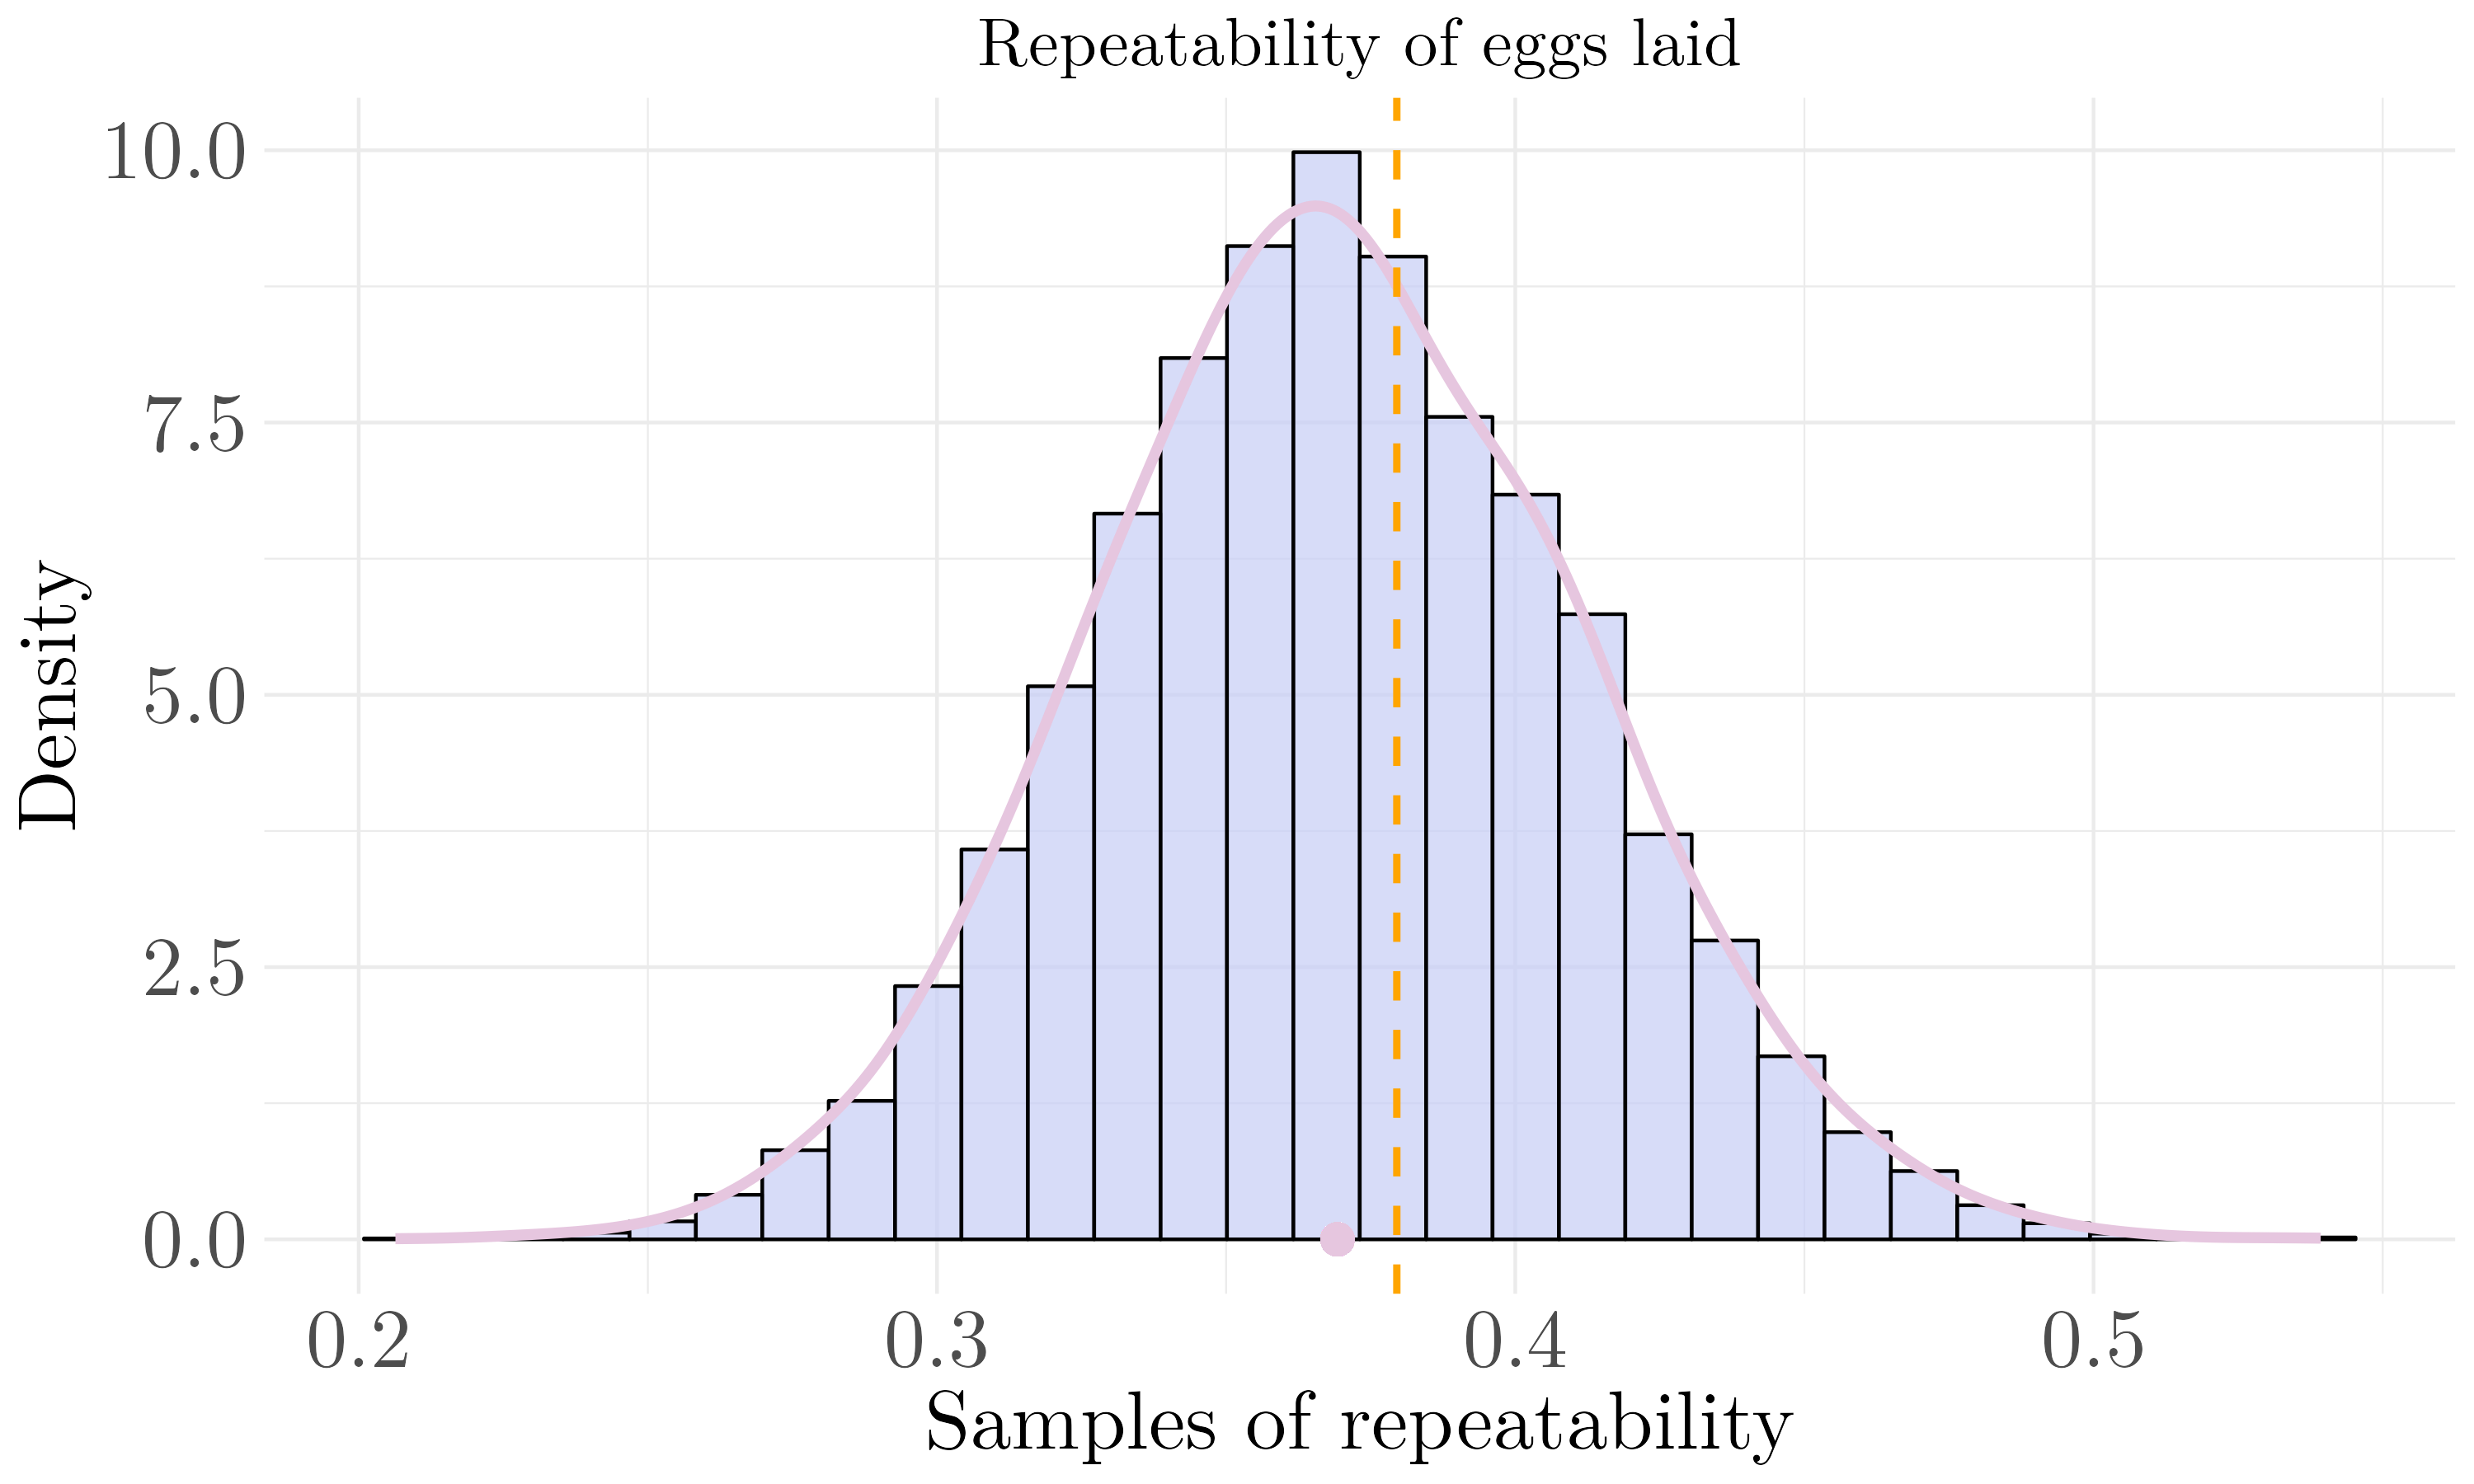
\includegraphics[width=1\linewidth]{Figures/Stoffel Comparison/Heritability_egg_poisson.png}
  \caption[Estimated repeatability of eggs laid by female beetles]{Histogram with repeatability values sampled from the posterior distribution for eggs laid by female beetles from BVI method, with the mean of the samples denoted by a pink circle. The estimate from the \texttt{rptR} package marked as a dashed line with orange color.}
  \label{fig:heritability_eggs_poisson}
\end{figure}
\noindent Importantly, note that the estimates from the BVI method will vary each time a model is fit, as it is stochastic. In this comparison, we only fit a single Bayesian GLMM with the BVI method. Therefore, it could be that another fit from the BVI method might align closer with the results of Stoffel and Nakagawa, but it could also be further off. 

% \section{Comparing the BVI method with \texorpdfstring{$R^2$}{Lg}-induced Dirichlet decomposition priors and Generalized Decomposition Priors on \texorpdfstring{$R^2$}{Lg}}
\section{Comparing the BVI method with Dirichlet and Generalized Decomposition Priors on \texorpdfstring{$R^2$}{Lg}}
To explore other possible relative variable importance tools in the Bayesian framework, we have discussed R2D2 and GDR2 priors in \Cref{sec:R2D2} and \Cref{sec:r2d2method}. We now present the results of applying the R2D2 and GDR2 priors to a linear regression, and see how they can be interpreted as relative importance measures. The results are compared to the sampled posterior relative importances computed by the BVI method and the LMG method serves as a robust benchmark for all methods. Please note once again that the R2D2 and GDR2 priors are originally developed for prediction models, and that the results presented here are based on our interpretation of how the R2D2 and GDR2 priors can be used for relative importance. The theoretical importances for uncorrelated covariates are found in \eqref{eq:RI_R2D2} and the theoretical $R^2$ for all correlation levels are found in \Cref{table:r2values_r2d2}. 
\begin{figure}[H]%\ContinuedFloat
  \centering
  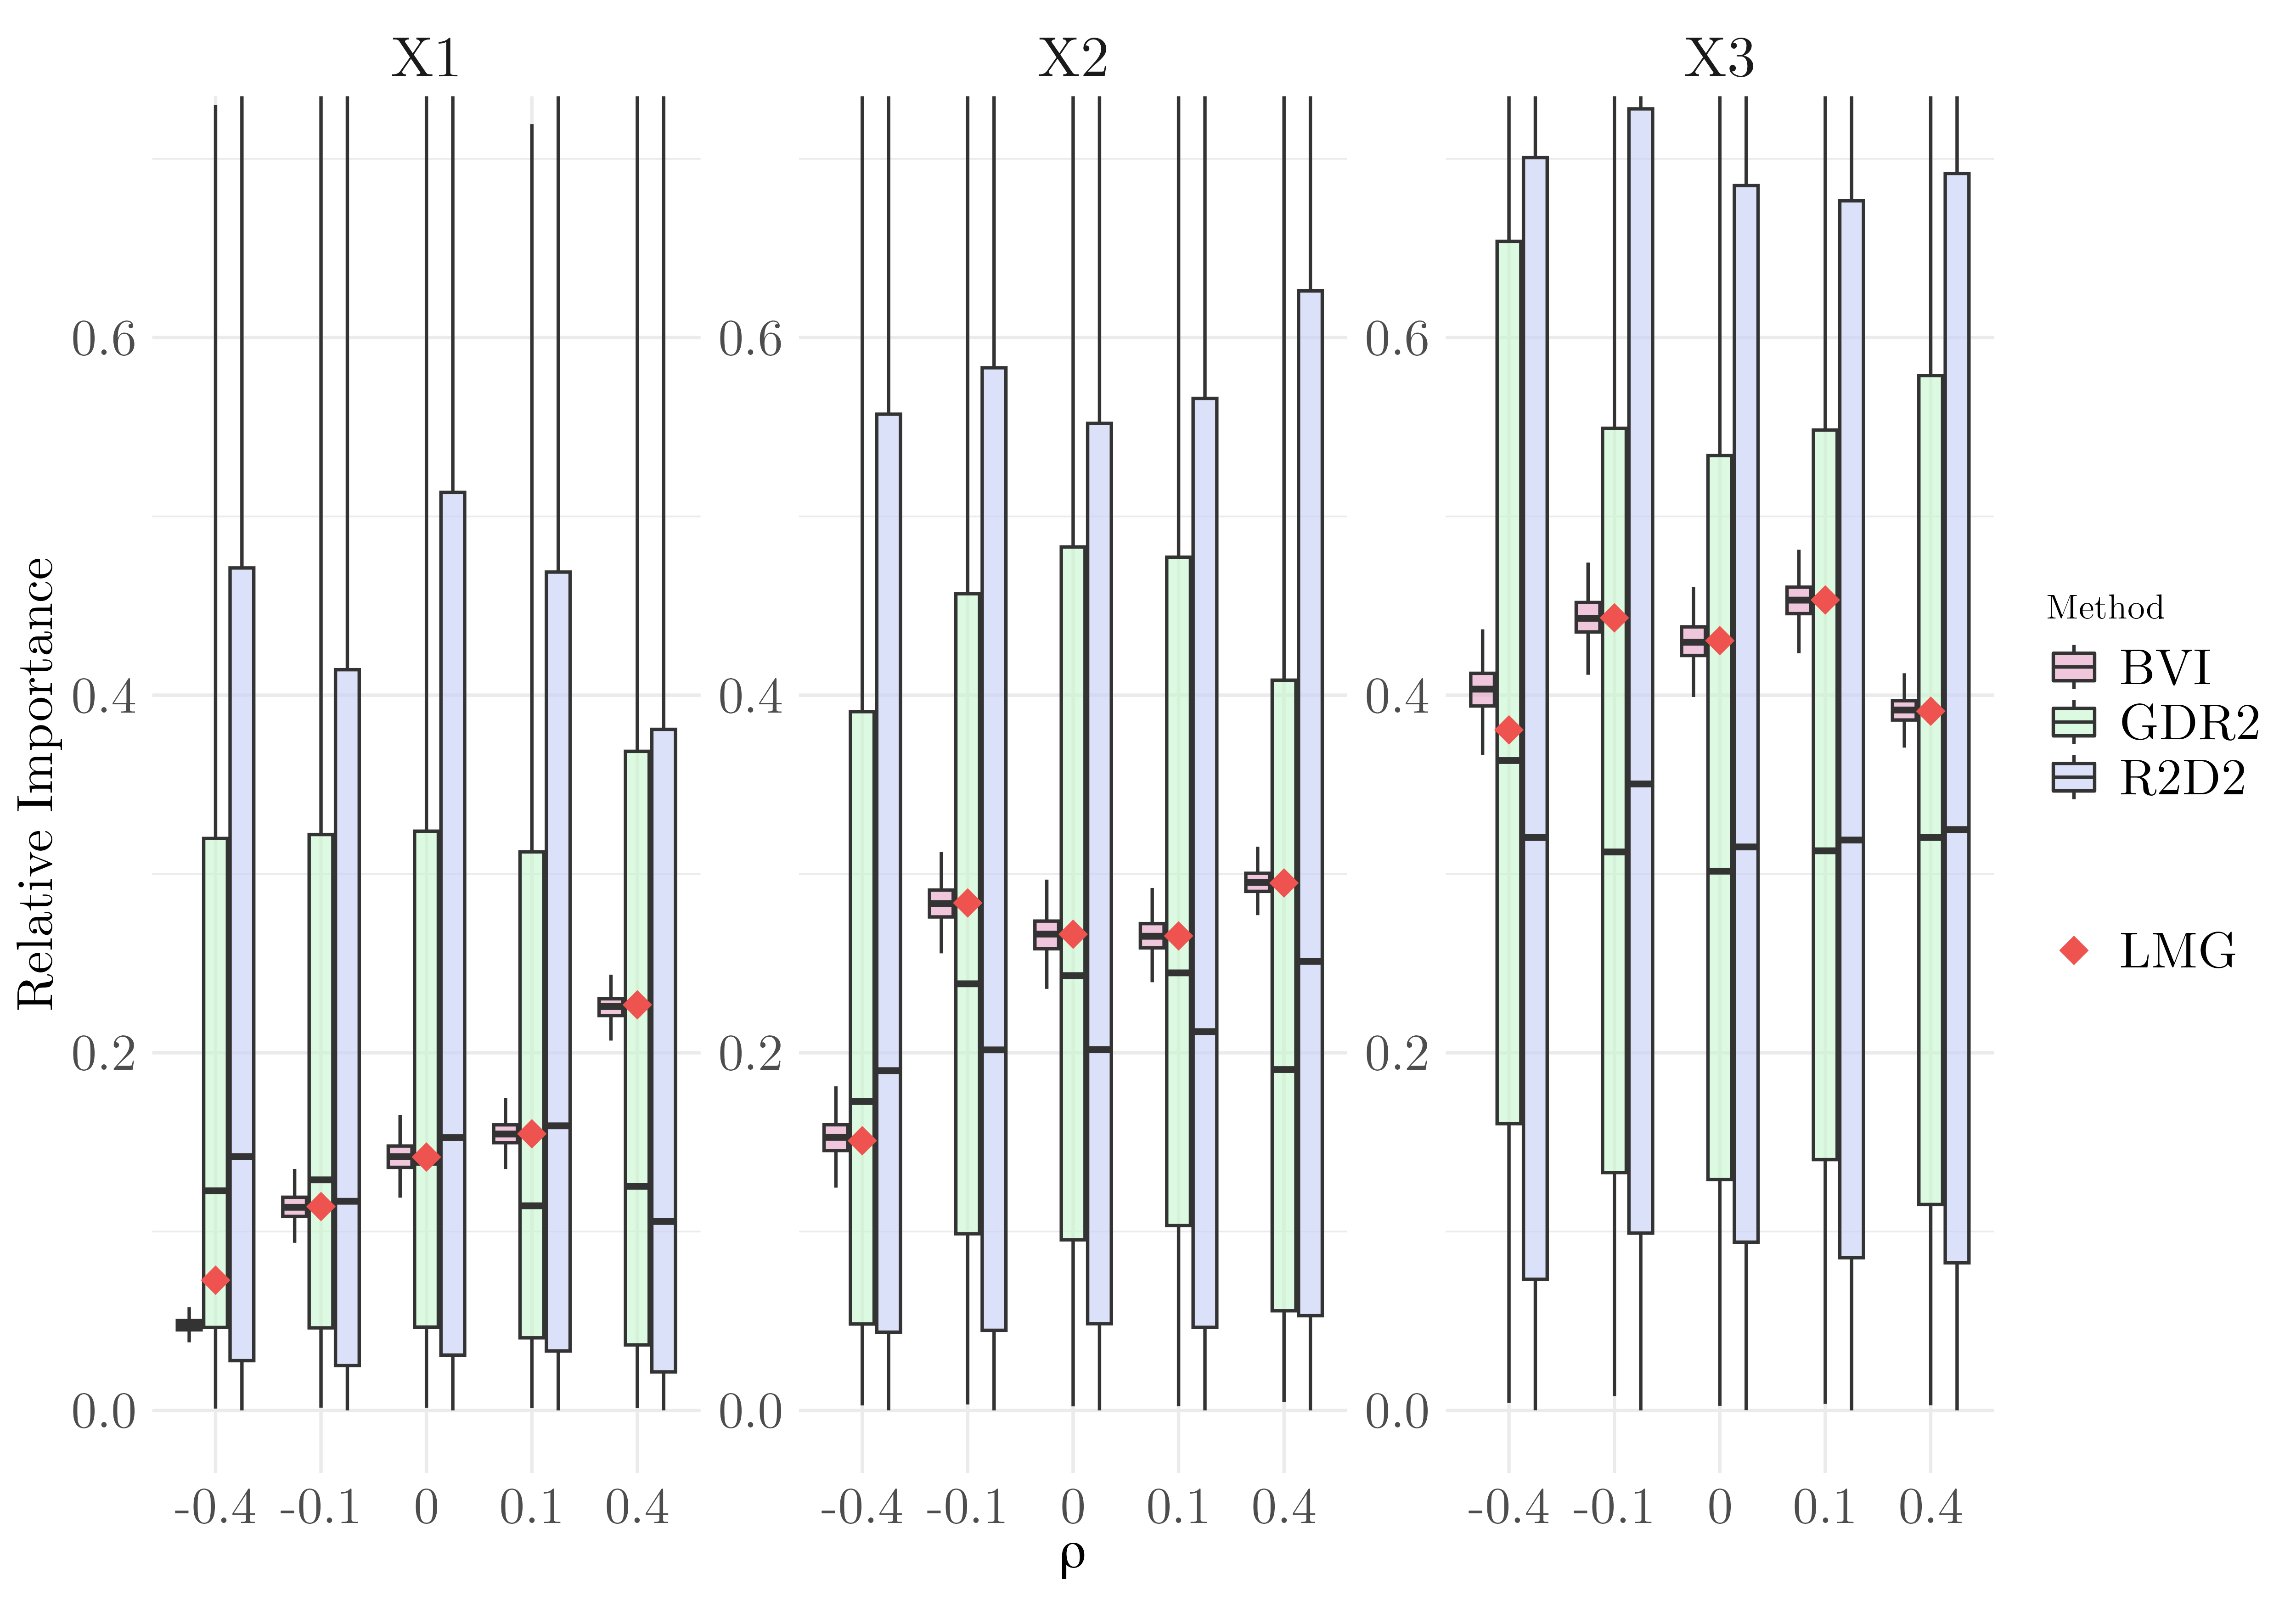
\includegraphics[width=1\linewidth]{Figures/R2D2_BVI_Comparison/R2D2_BVI_boxplot.png}
  \caption[Comparison of the relative importance from the BVI method and the shrinkage prior methods]{Box plots of the relative importance distributions for $X_1$, $X_2$ and $X_3$ for varying correlation levels by the R2D2, GDR2 and BVI methods. The correlation levels $\rho$ are denoted along the x-axis, and the red diamond represents the relative variable importance calculated from the LMG method.}
  \label{fig:r2d2_importance}
\end{figure}
\noindent The first thing one notices from the posterior relative importance distributions (\Cref{fig:r2d2_importance}), is that the spread from the R2D2 method is larger than the spread of the GDR2 method, which again is significantly larger than the spread of the BVI method. In the box plots, the $25$th and $75$th quantiles define the interval of each box. The mean values of the relative importance distributions for the R2D2 and GDR2 methods do not seem to follow any pattern at all for varying correlation. They are more similar across correlation levels for all covariates, and do not adjust for correlation as the benchmark LMG method. Although it is hard to find patterns and the R2D2 and GDR methods give very flexible results, it becomes clear from they grasp the larger aspects, in that $X_3$ is estimated to be the covariate with the largest variance contribution, followed by $X_2$ and lastly $X_1$. The BVI method is in close agreement with the LMG method, with deviation for $X_1$ and $X_3$ when $\rho=-0.4$. Overall the BVI and LMG methods follow the same pattern for varying correlation, as we expect and have previously discussed.
\begin{figure}[H]%\ContinuedFloat
  \centering
  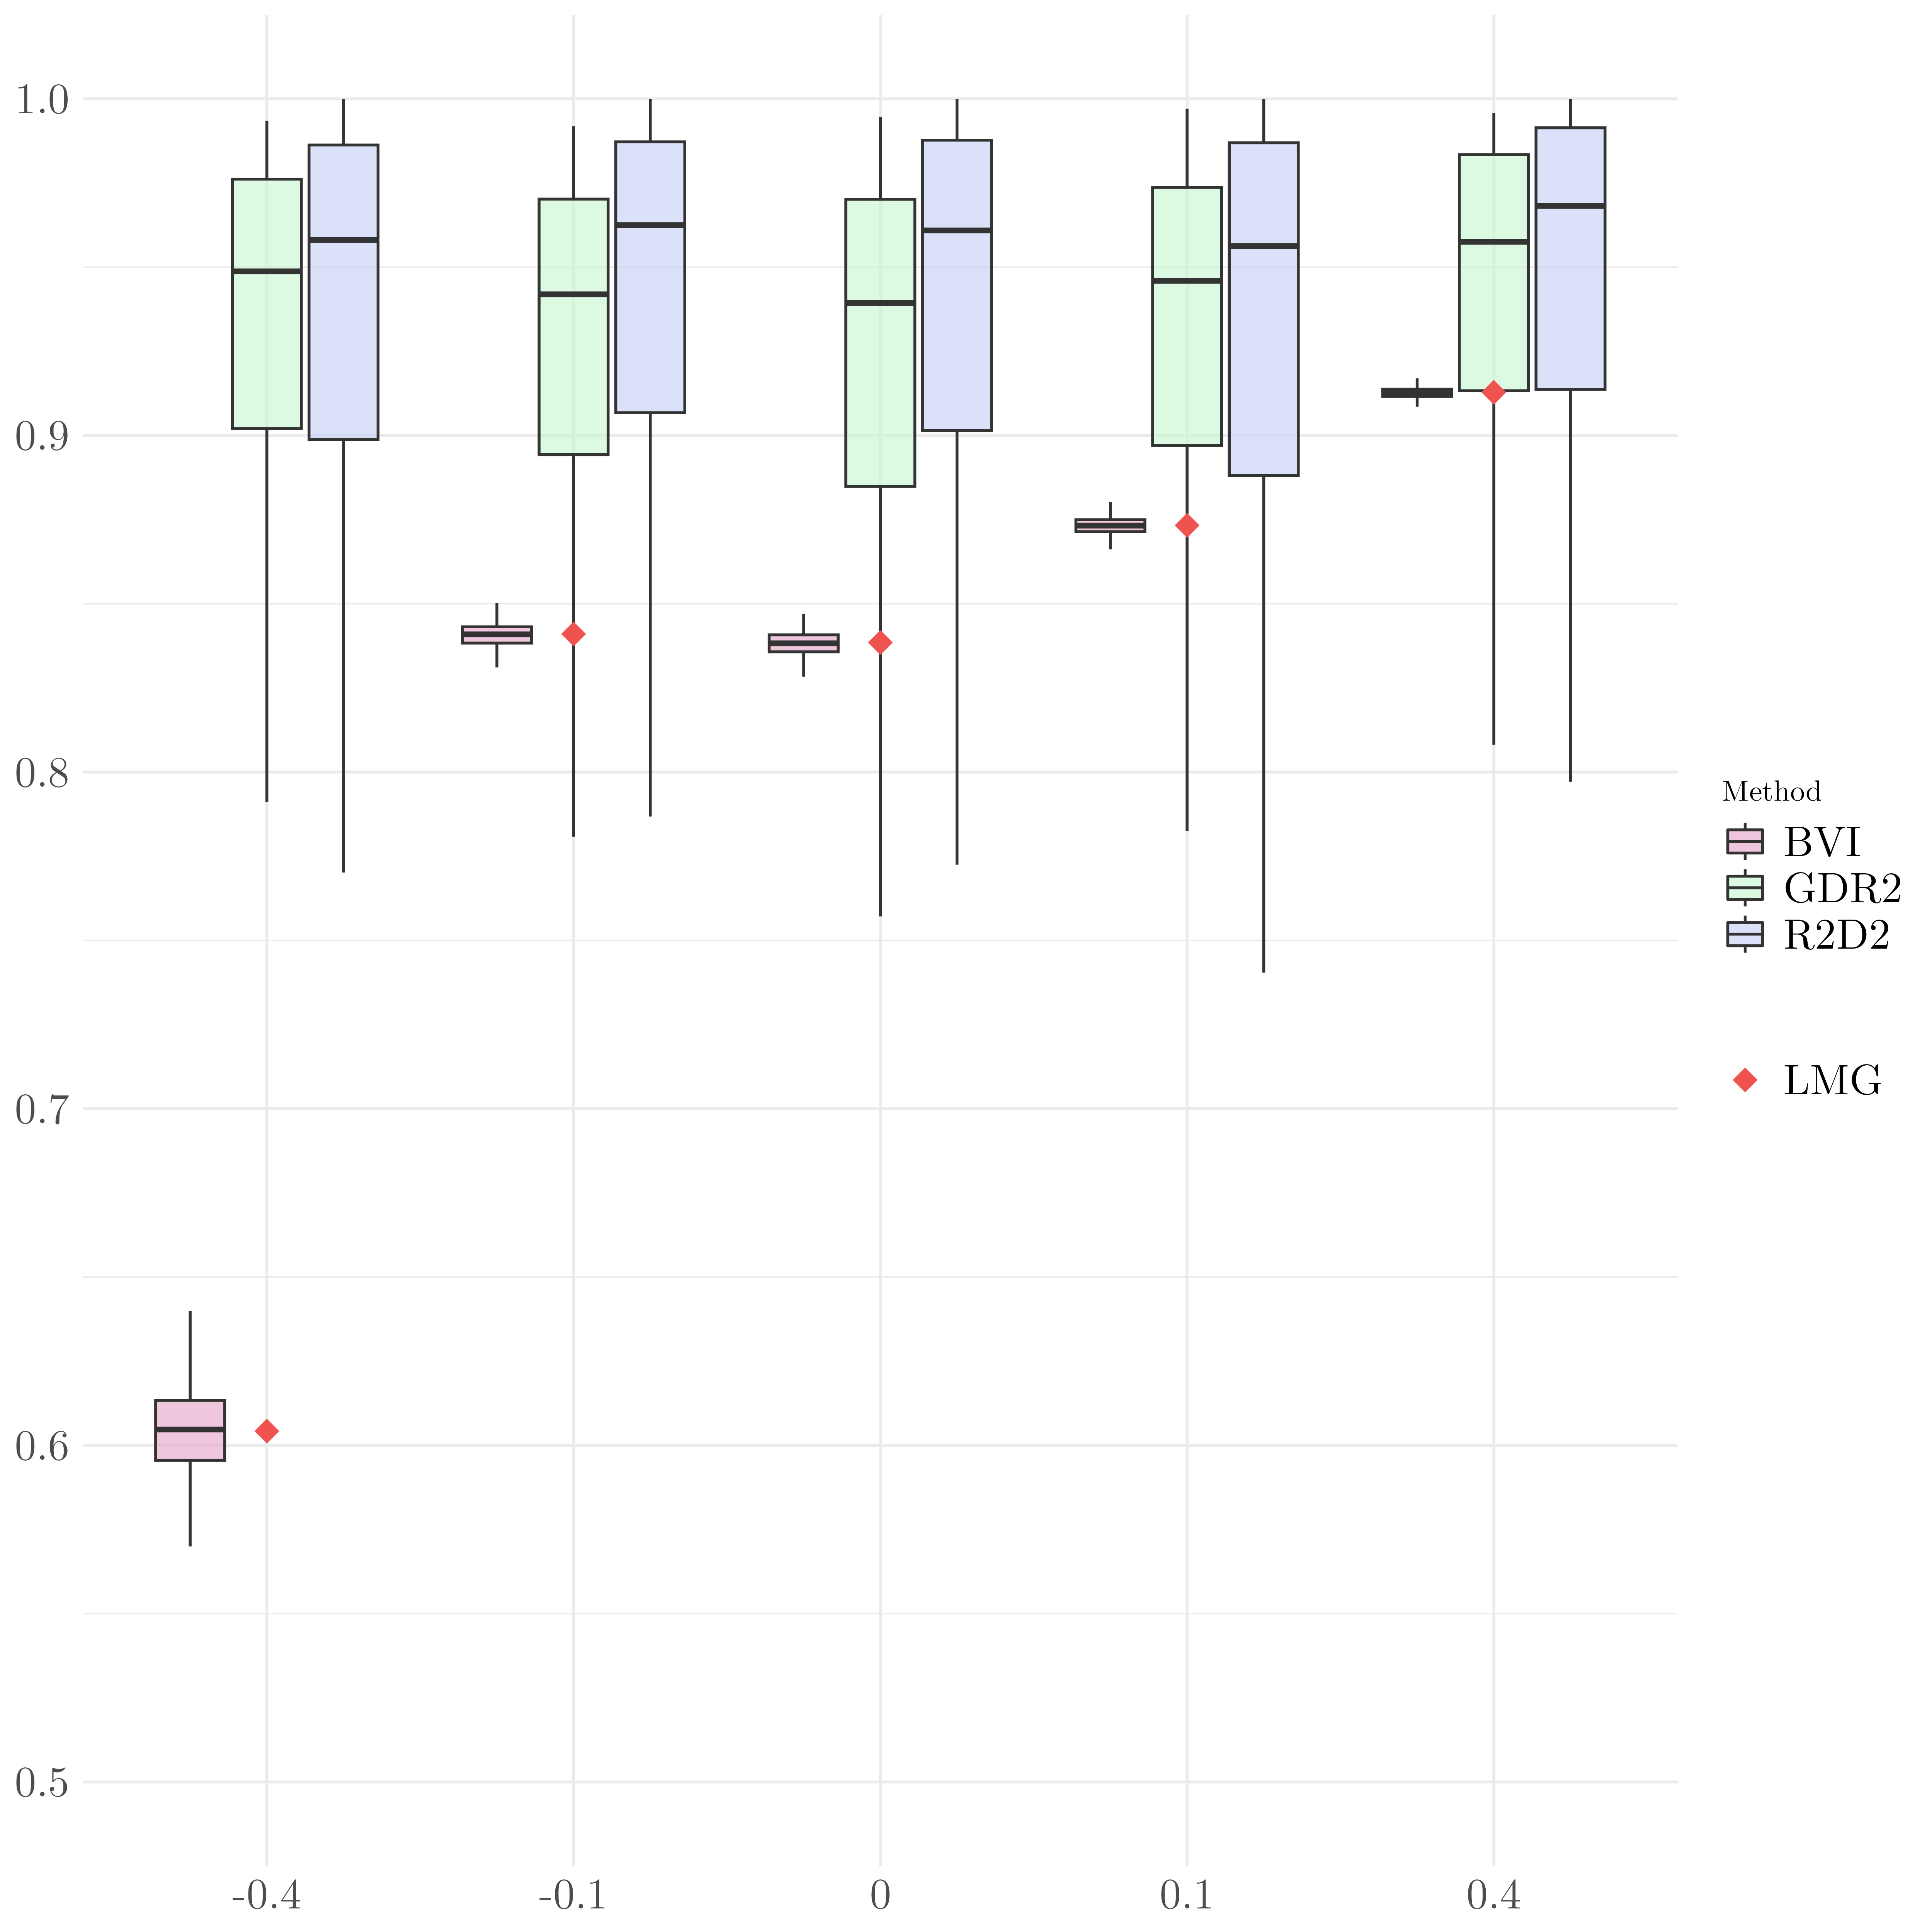
\includegraphics[width=1\linewidth]{Figures/R2D2_BVI_Comparison/R2D2_BVI_R2_plot.png}
  \caption[Comparison of the marginal $R^2$ from the BVI method and the shrinkage prior methods]{Box plots of the estimated $R^2$ distributions for varying correlation levels $\rho$ for the R2D2, GDR2 and BVI methods. The correlation levels $\rho$ are denoted along the x-axis, and the red diamond represents the relative variable importance calculated from the LMG method.}
  \label{fig:r2d2_r2}
\end{figure}
\noindent The estimated posterior marginal $R^2$ distributions for the R2D2 and GDR2 priors (\Cref{fig:r2d2_r2}) are uniform across the correlation levels, and significantly larger than both the estimates of the BVI and LMG methods. For the $R^2$, the spread of the R2D2 and GDR2 methods are quite similar, with both being much larger than that of the BVI method. Overall, the R2D2 and GDR2 estimates a much larger $R^2$ than the BVI and LMG methods, and the means deviate quite much from the expected values. The BVI method is consistent with the LMG method, and they both follow the expected pattern of the $R^2$. For the expected $R^2$, the BVI and LMG methods seem to align closely with the expectation, with a small deviation for both methods when $\rho=0$.
\\
\\
As the R2D2 and GDR2 methods are not specifically relative variable importance measures, one should also interpret the results with this in mind. The development of the R2D2 and GDR2 priors have been done to produce robust predictions for high dimensional linear regression models, and the results presented here are therefore not an evaluation of the R2D2 and GDR2 priors as relative importance measures. Moreover, the interpretation made to obtain these results was made by the author, and the results should be taken with caution. The main motivation behind this comparison was to explore other possible relative importance measures in the Bayesian framework, as this is a small field with few available methods. 




